\chapter[Sociedade, política e espaço urbano de Salvador em seu contexto (1889-1930)]{Sociedade, política e espaço urbano de \\Salvador em seu contexto (1889-1930)}\label{cap:1}

Neste capítulo, será esboçado um panorama da sociedade, da política e do espaço urbano de \index{Salvador}Salvador, inserido nos contextos global e nacional de sua época. Será dada especial atenção aos aspectos demográfico, político e cultural da cidade, à sua estratificação social e à configuração de seu espaço urbano.

Antes de chegar às contradições e conflitos sociais próprios da sociedade soteropolitana, é preciso compreender sua inserção no contexto nacional, e para chegar até ele é preciso entender igualmente o contexto internacional; é só por meio desta inserção que se tornará possível compreender algumas das contradições econômicas, políticas e sociais mais importantes do período. Já outras poderão ser compreendidas mediante a simples articulação de fatores verificados em escala municipal, estadual ou nacional, mas mesmo estes relacionam-se em algum nível com questões internacionais. Nesta escala, a análise terá de ser, forçosamente, econômica e geopolítica.

Em seguida, será desenhado um panorama da política brasileira e da inserção do Brasil na economia global durante o período, pois a inserção soteropolitana no contexto é fortemente determinada pelas turbulências da época. Será dada especial atenção à estratificação social brasileira e ao desenvolvimento das grandes cidades no país durante o período, por comporem um ambiente em que ideias e profissionais circulavam com grande facilidade e formarem um quadro ideológico e prático comum a partir das propostas de ``melhoramentos'' urbanos.

Posteriormente, será feita uma análise da sociedade e da política baianas, cada qual numa seção específica. O foco estará na inserção de Salvador na economia global, na sua demografia, na sua estratificação social (com algumas discussões específicas sobre a intelectualidade e a classe trabalhadora) e as interfaces entre a cultura e o uso dos espaços públicos. Será feita também uma descrição das instituições políticas estaduais e municipais, por interferirem diretamente na produção do espaço urbano, além de uma caracterização dos agentes da política baiana e de suas interações e conflitos.

Por fim, vistos todos os fatores que, nesta pesquisa, se considera condicionantes da produção do espaço urbano no período estudado, será possível adentrar na dinâmica da produção do espaço urbano soteropolitano com base nos recenseamentos de 1872 e 1920, que detalham a população soteropolitana e o uso imobiliário do espaço urbano com razoável detalhamento. Além disso, será dada especial atenção ao regime de terras vigente na cidade e às intervenções no espaço urbano, com destaque para as reformas promovidas durante os governos de José Joaquim Seabra (1912-1924).

\section{Contexto internacional}\label{sec:1.1}

Costuma-se estabelecer como marco histórico da passagem do século XIX para o XX o novo \index{imperialismo}imperialismo colonialista pactuado na \index{imperialismo!Conferência de Berlim (1884-1885)}Conferência de Berlim (1884-1885), mas tal marco coloca em segundo plano questões importantes mais remotas, definidoras de tendências desta época. O período escolhido para esta pesquisa está inserido numa longa e turbulenta linha de acontecimentos inserida num ciclo que vai de 1870 a 1929 \cite{bernardo_fascismo_2003,bukharin_imperialismo_1986,
hobsbawm_empire_1989,hobsbawm_extremes_1995,hobson_imperialism_1902,
hobson_capitmoderno_1983,KROPOTKIN1901,lenin_imperialismo_1987,luxemburg_acumula_1985,
morris_magnatas_2010}, iniciado com a Guerra Franco-Prussiana (19 de julho de 1870 - 10 de maio de 1871) e encerrado com a crise de 1929. Para entender a dinâmica deste ciclo, é preciso compreender seus fatores principais e extrair deles os elementos que interessam ao recorte temporal e espacial da presente pesquisa. 

\subsection{Precedentes: as unificações políticas e a crise econômica global de 1873-1896}

Dois fatores preponderam como antecedentes históricos relevantes, em escala global, do período escolhido para o estudo: as \index{unificação ou reunificação política}\textit{unificações e reunificações políticas} de países europeus anteriormente fragmentados, concluídas nos anos 1880; e a \index{crises econômicas!crise de 1873-1896}\textit{crise econômica de 1873-1896}.

O \index{Itália!risorgimento@\textsl{risorgimento}}\textit{risorgimento} da \index{Itália}Itália foi um longo processo, iniciado com a confirmação da partição da \index{Itália}Itália pelo \textit{Congresso de Viena} (1815) e concluído com a tomada de Roma (1871). Levantes e insurreições contra o domínio austríaco sobre a Itália já aconteciam desde 1820 sob a influência dos \index{Itália!risorgimento@\textsl{risorgimento}!carbonários}\textit{carbonários}, mas foram a \index{Itália!risorgimento@\textsl{risorgimento}!Insurreição de 1830}\textit{Insurreição de 1830} e a \index{Itália!risorgimento@\textsl{risorgimento}!Primeira Guerra Italiana de Independência}\textit{Primeira Guerra Italiana de Independência} (1848-1849), esta última com presença marcante do movimento \index{Itália!risorgimento@\textsl{risorgimento}!\textit{Giovane Italia}}\textit{Giovane Italia}, os primeiros movimentos políticos a pautar seriamente a questão. A \index{Itália!risorgimento@\textsl{risorgimento}!Segunda Guerra Italiana de Independência}\textit{Segunda Guerra Italiana de Independência} (1859), iniciada pelo Reino da Sardenha governado pelo rei \index{Itália!risorgimento@\textsl{risorgimento}!Vítor Emanuel II}\textit{Vítor Emanuel II} e pelo primeiro-ministro \index{Itália!risorgimento@\textsl{risorgimento}!Camillo Benso, Conde de Cavour}\textit{Camillo Benso, Conde de Cavour}, trouxe os primeiros resultados expressivos para a unificação italiana com a anexação do Reino das Duas Sicílias ao Reino da Sardenha. No ano seguinte, o Reino da Sicília anexou, com o beneplácito da \index{França}França e da \index{Grã-Bretanha}Grã-Bretanha, o Ducado de Parma, o Ducado de Modena, o Grão-Ducado da Toscana e os Estados Papais; em troca, a França anexou a Saboia e Nice. Já em 17 de março de 1861 o parlamento sardo proclamou a mudança do nome do Reino da Sardenha para Reino da Itália, e proclamou \index{Itália!risorgimento@\textsl{risorgimento}!Vítor Emanuel II}Vítor Emanuel como \textit{Rei da Itália}. Restavam, para completar o quadro, o Reino Lombardo-Vêneto e o território restante dos antigos Estados Papais; o primeiro foi anexado em 1866 depois da \index{Itália!risorgimento@\textsl{risorgimento}!Terceira Guerra Italiana de Independência}\textit{Terceira Guerra Italiana de Independência} (1866), e o segundo depois da \index{Itália!risorgimento@\textsl{risorgimento}!captura de Roma}\textit{captura de Roma} (1870) \cite{hobsbawm_capital_1977}.

A \index{EUA!Guerra de Secessão}\textit{Guerra de Secessão} nos \index{EUA}EUA (12 abr. 1861 - 22 jun. 1865), ao mesmo tempo em que reunificou os \index{EUA}EUA, colocou-os sob a hegemonia dos estados industriais do \index{EUA!Norte}Norte, extinguiu a escravidão nos estados do \index{EUA!Sul}Sul e facilitou enormemente a conflagração de guerras de conquista contra os povos indígenas ao \index{EUA!Oeste}Oeste. 

A \index{Alemanha!unificação da Alemanha}\textit{unificação da Alemanha} em 18 de janeiro de 1871 foi o ápice de um processo iniciado em 1862. A vitória da \index{Alemanha!Confederação da Alemanha do Norte}Confederação da Alemanha do Norte sobre a \index{França}França de \index{Napoleão III}Napoleão III na \index{Guerra Franco-Prussiana}Guerra Franco-Prussiana, resultante, entre outras coisas, do enorme avanço técnico e industrial experimentado durante a segunda metade do século XIX nos pequenos reinos (em especial a \index{Alemanha!Prússia}Prússia) que viriam a formar a \index{Alemanha}Alemanha unificada.  A tomada da \index{Alsácia-Lorena}Alsácia-Lorena aos franceses, outro resultado da guerra, garantiu à \index{Alemanha}Alemanha a satisfação de velhas aspirações nacionalistas, uma vantagem estratégica (afastar do \index{Alemanha!Reno}Reno a fronteira com a \index{França}França e fixá-la na cordilheira dos \index{França!Vosges}Vosges, obstáculo natural militarmente mais eficaz \cite{eckhardt_alsace_1918}) e uma vantagem econômica (\index{matérias-primas!carvão}carvão e \index{matérias-primas!ferro}ferro, fundamentais para uma \index{indústria}indústria ainda baseada no \index{energia!vapor}vapor e, posteriormente, na \index{energia!energia termelétrica}energia termelétrica \cite{brooks_alsace_1917}), mas assegurou permanente animosidade entre os dois países. O \index{Áustria!Império Austro-Húngaro}Império Austro-Húngaro, que disputara ferozmente com a \index{Alemanha!Prússia}Prússia a hegemonia sobre a \index{Alemanha!Confederação Alemã|seealso{Confederação da Alemanha do Norte}}Confederação Alemã até então, ficou para trás, malgrado seus enormes avanços tecnológicos \cite{schulze_engin_1996}, vivendo em suas últimas décadas (1900-1918) notável degeneração institucional. 

Estes processos de unificação (\index{Alemanha}Alemanha e \index{Itália}Itália) e reunificação (\index{EUA}EUA) criaram as condições para que a hegemonia política global da \index{Grã-Bretanha}Grã-Bretanha no século XIX fosse desafiada. Pode-se dizer que parte de seu sucesso econômico e político nos três primeiros quartos do século se deveu à fragmentação política de outros países que poderiam ser seus sérios concorrentes nos campos geopolítico e econômico; para azar dos britânicos, os processos de unificação e reunificação foram animados por elementos ideológicos favorecedores do expansionismo, do anexionismo e da disputa geopolítica internacional. Na medida em que \index{Itália}Itália e \index{Alemanha}Alemanha foram agrupadas em torno de fronteiras engenhosamente justificadas por meio da \textit{invenção de tradições} \cite{hobsbawm_prodtrad_2012} e de um \index{nacionalismo}nacionalismo reforçado por \index{nacionalismo!nacionalismo linguístico}argumentos linguísticos e \index{nacionalismo!racismo}``raciais'' \cite{hobsbawm_transfnac_2011}, criam para si não apenas os instrumentos necessários a uma coesão social de tipo novo, cujos efeitos seriam percebidos na \index{imperialismo!Conferência de Berlim (1884-1885)}Conferência de Berlim, mas igualmente a justificativa para uma ``vontade de poder'' de caráter expansionista \cite{rocker_nacult_1954} cujos efeitos mais nefastos só seriam percebidos quase meio século depois. A arquitetura pública e os monumentos cívicos tiveram papel fundamental nesta invenção de tradições, na medida em que a ornamentação dos prédios, o simbolismo dos monumentos, a escolha dos motivos, tudo, enfim, remetia às tradições que se pretendia inventar ou reinventar \cite{hobsbawm_prodtrad_2012}.

Nos \index{EUA}EUA, as mesmas teorias \index{nacionalismo!nacionalismo linguístico}linguísticas e \index{nacionalismo!racismo}``raciais'' se somaram, para os mesmos efeitos, à ideologização das \textit{guerras de fronteira com os índios} como um dos fundamentos da democracia \cite{turner_frontier_1920} e à vaga noção de um \index{nacionalismo!``destino manifesto'' (teoria)}``destino manifesto'', de caráter dito ``civilizatório'', dos estadunidenses de ascendência anglo-saxã \cite{brown_mandest__1980,horsman_mandest_1981}, envolvendo com este véu ideológico a \index{imperialismo!Guerra Hispano-Americana}\textit{Guerra Hispano-Americana} (1898), as \index{imperialismo!Guerras das Bananas}\textit{Guerras das Bananas} (1898-1934) e a consequente conquista de Cuba, das Filipinas, de Porto Rico e da ilha de Guam.

Outro fator de extrema relevância: a \textit{\index{crises econômicas!crise de 1873-1896}crise de 1873-1896}, duas décadas de estagnação financeira e comercial menos conhecidas que a \index{crises econômicas!crise de 1929}crise de 1929, mas igualmente importantes na história econômica global \cite{Fels1949,Fels1951,hobsbawm_empire_1989,Musson1959,Rezneck1950,Sprague1910,Persons1920}. 

As indenizações de guerra impostas à \index{França}França pela \index{Alemanha}Alemanha como resultado da \index{Guerra Franco-Prussiana}Guerra Franco-Prussiana baquearam severamente a \index{especulação imobiliária}especulação imobiliária em Paris (via \index{Georges-Eugène Haussmann}\index{Haussmann|seealso{Georges-Eugène Haussmann}}Haussmann), enquanto na \index{Alemanha}Alemanha os bancos e bolsas de valores, por sua vez, lançaram-se à especulação desenfreada graças ao dinheiro destas indenizações; é o tempo a que os alemães chamam \textit{\index{Alemanha!Gründerzeit@\textsl{Gründerzeit}}Gründerzeit}, ou seja, o ``tempo dos empresários'', quando mesmo as mais descaradamente fraudulentas iniciativas e os mais absurdos negócios encontravam investidores com enorme facilidade \cite[p.~61]{hobsbawm_capital_1977}. Na \index{Áustria}Áustria, grande parceira econômica da \index{Alemanha}Alemanha, o influxo de dinheiro criou condições para a reconstrução de \index{Áustria!Viena}Viena, e para a \index{especulação imobiliária}especulação imobiliária sem precedentes que levou ao primeiro \index{crises econômicas!crack@\textit{crack}}\textit{crack} da série, em 8 de maio de 1873, rapidamente espraiado pelas bolsas de \index{Alemanha!Berlim}Berlim e \index{França!Paris}Paris.

Nos \index{EUA}EUA, a bolha criada pela enorme \index{transportes!expansão ferroviária|seealso{ferrovias}}expansão ferroviária estourou: um dos grandes financiadores do Norte na \index{EUA!Guerra de Secessão}Guerra de Secessão, o banco \index{carteis e trustes!EUA!Jay Cooke \& Co.}Jay Cooke \& Co., abriu falência em 18 de setembro de 1873, como consequência de sua dificuldade em negociar ações da \index{transportes!ferrovias!Northern Pacific Railroad}Northern Pacific Railroad após mais uma derrota do exército estadunidense para os \index{EUA!Oeste!\textit{hunkpapa}}\textit{hunkpapa} liderados por \index{EUA!Oeste!Touro Sentado}Touro Sentado \cite[p.~241-242]{utley_frontier_1973}; a falência desencadeou uma crise na \index{bolsas de valores!Bolsa de Nova Iorque}Bolsa de Nova Iorque, fechada por dez dias para conter as quebras. Várias companhias ferroviárias e bancos americanos faliram. 

Como a especulação em torno das ferrovias estadunidenses envolvia a \index{indústria!siderurgia}siderurgia e diversos bancos alemães, britânicos e franceses, já combalidos pela \index{crises econômicas!crise austríaca}crise austríaca, a crise voltou a se espalhar pelo globo, e retornou com força total noutros dois \index{crises econômicas!cracks em 1882 e 1884}\textit{cracks} em 1882 e 1884.

Para piorar a situação, embora o comércio e as finanças vivessem um período de franca \index{crises econômicas!depressão}depressão, as inovações técnicas na \index{indústria!produção industrial}produção industrial pautaram um ritmo crescente na \index{produtividade}produtividade \cite{hobsbawm_empire_1989}, seja nos setores considerados \textit{\index{condições gerais da produção}condições gerais da produção} \cite[p.~155-162]{BERNARDO1991}, seja em setores de menor impacto sobre os processos produtivos. Um exemplo: a produção de \index{matérias-primas!ferro}ferro nos cinco maiores países produtores passou de 11 milhões de toneladas para 23 milhões entre 1870 e 1890, enquanto a produção global de \index{matérias-primas!aço}aço no mesmo período saltou de meio milhão de toneladas para 11 milhões \cite[p.~35]{hobsbawm_empire_1989}.

Uma das consequências da crise destes anos foi a \index{onda migratória}\textit{onda migratória da} \index{Europa}\textit{Europa para a }\index{América}\textit{América}, sensivelmente aumentada na década de 1880 (cf. \autoref{tab:emigra} (p. \pageref{tab:emigra}) e \autoref{tab:imigra} (p. \pageref{tab:imigra})).

\begin{table}[!htp]
\centering
\IBGEtab{
\caption{Emigração europeia 1846-1930, por país de origem (em milhões de pessoas)}\label{tab:emigra}}
{\begin{tabular}{cccccc}
\toprule
Ano & Total & Reino Unido & Espanha e Portugal & Alemanha e Áustria & Outros \\
\midrule \midrule
1846-1850 & 0,5 & 0,2 & -- & 0,2 & 0,1 \\
1851-1860 & 2,2 & 1,3 & 0,85 & 0,65 & 0,2 \\
1861-1870 & 2,6 & 1,6 & 0,1 & 0,7 & 0,2 \\
1871-1880 & 3,1 & 1,85 & 0,15 & 0,75 & 0,35 \\
1881-1890 & 7,0 & 3,25 & 0,75 & 1,8 & 1,2 \\
1891-1900 & 6,2 & 2,15 & 1,0 & 1,25 & 1,8 \\
1901-1910 & 11,3 & 3,15 & 1,4 & 2,6 & 4,15 \\
1911-1920 & 7,6 & 2,6 & 1,7 & 0,9 & 2,4 \\
1921-1930 & 6,6 & 2,15 & 1,6 & 1,1 & 1,75 \\
\bottomrule
\end{tabular} }
{ \fonte{Elaboração do autor, com dados recolhidos n'\textbf{A economia política do imperialismo} de Michael \citeonline[p.~127]{brown_imper_1978}. } }
\end{table}


\begin{table}[!htp]
\centering
\IBGEtab{
\caption{Imigração em países de colonização europeia 1846-1930, por país de destino (em milhões de pessoas)}\label{tab:imigra}}
{\begin{tabular}{|ccccccc|}
\hline
Ano & Total & EUA & Canadá & Argentina e Brasil & Austrália e Nova Zelândia & Outros \\
\hline
1846-1850 & 1,6 & 1,25 & 0,25 & -- & -- & 0,1 \\
1851-1860 & 3,4 & 2,6 & 0,3 & 0,05 & 0,05 & 0,4 \\
1861-1870 & 3,4 & 2,3 & 0,3 & 0,2 & 0,2 & 0,4 \\
1871-1880 & 4,0 & 2,8 & 0,2 & 0,5 & 0,2 & 0,3 \\
1881-1890 & 7,5 & 5,2 & 0,4 & 1,4 & 0,3 & 0,2 \\
1891-1900 & 6,4 & 3,7 & 0,2 & 1,8 & 0,45 & 0,25 \\
1901-1910 & 14,9 & 8,8 & 1,1 & 2,45 & 1,6 & 0,95 \\
1911-1920 & 11,1 & 5,7 & 1,1 & 2,0 & 1,0 & 1,3 \\
1921-1930 & 8,7 & 4,0 & 1,0 & 2,15 & 0,7 & 0,85 \\
\hline
\end{tabular} }
{ \fonte{Elaboração do autor, com dados de \citeonline[p.~127]{brown_imper_1978}.} }
\end{table}

Conquanto inserida no contexto das crises econômicas, a onda migratória pode ser explicada de forma mais imediata e analítica por causas mais próximas: a disparidade de renda entre países de origem (com renda \textit{per capita} mais baixa) e destino (com renda \textit{per capita} mais alta); as altas taxas de crescimento populacional natural nos países de origem, que resultaram em aumento da densidade populacional na forma -- explicada por outras razões -- de urbanização acelerada e aumento da pressão por equipamentos coletivos (habitação, transporte, escolas etc.), servindo então as más condições urbanas como pressão emigratória rumo a países com baixa densidade populacional; e um declínio sustentado nos custos de transportes terrestres e marítimos entre 1870 e 1914, fazendo destes 44 anos o período ``em que o movimento internacional de pessoas foi menos restrito que em qualquer outro período dos tempos modernos'' \cite[p.~616]{heitger_migration_1993}.

Outra das consequências da crise foi a confirmação do \index{declínio da hegemonia britânica!Grã-Bretanha}declínio da hegemonia britânica sobre a economia global; embora o papel dos capitais britânicos na economia global ainda fosse inquestionável \cite{goetzmann_british_2006,rippy_britlat_1954,stone_british_1977}, sua produção industrial, embora crescesse, fazia-o em taxas declinantes, e o desenvolvimento de suas indústrias nos ramos de ponta como a química e a engenharia elétrica estava claramente a reboque do que se fazia na \index{Alemanha}Alemanha e nos \index{EUA}EUA \cite[p.~207]{Musson1959}. 

Uma última consequência da crise foi a criação dos \index{carteis|seealso{carteis e trustes}}\textit{carteis} na \index{Alemanha}Alemanha, dos \index{trusts|seealso{carteis e trustes}}\textit{trusts} nos \index{EUA}EUA e de outras formas de organização monopolista de empresas, apontadas por \citeonline[p.~125-200]{hobson_capitmoderno_1983}, \citeonline[p.~16-29]{lenin_imperialismo_1987}, e \citeonline[p.~47-54]{bukharin_imperialismo_1986} como características de uma nova fase da economia mundial, precursoras daquilo que viriam a ser as grandes corporações e empresas do primeiro \index{pós-guerra}pós-guerra e também dos grandes conglomerados transnacionais do segundo \index{pós-guerra}pós-guerra.

\subsection{Imperialismo, colonialismo, carteis, trustes e a Primeira Guerra Mundial (1881-1914)} \label{sec:impercol}

Somente depois de entender estas preliminares é possível entender o imperialismo de um ponto de vista \textit{histórico}. Em que pesem as considerações de um \index{Schumpeter}\citeonline{schumpeter_imperialismo_1961} sobre incompatibilidades entre capitalismo e imperialismo, lançando o último na conta dos restos do absolutismo monárquico que persistiam no período, vista a questão pelo ponto de vista histórico, o imperialismo foi, no campo dos Estados-nação, uma das saídas encontradas para a crise dos anos 1870-1880, assim como os carteis e os trustes foram saídas para a mesma crise encontradas no campo das empresas; são dois lados da mesma moeda, funcionaram juntos e um não pode ser compreendido sem remissão ao outro.

Somente agora a \index{imperialismo!Conferência de Berlim (1884-1885)}Conferência de Berlim passa a fazer sentido como marco histórico de um período. Se anteriormente à crise dos anos 1870-1880 a relação dos países europeus com as sociedades africanas oscilou entre o comércio e a guerra de conquista \cite{ogot_hisaf5_2010,AJAYI2010}, neste período passam a ser de dominação territorial e anexação. É certo que fatores endógenos aos próprios Estados africanos, como as diversas lutas interestatais e intraestatais, e a superioridade europeia em diversos aspectos conjunturais (conhecimento geográfico do continente, saber médico contra doenças endêmicas e capacidade de sustentar guerras prolongadas), facilitaram enormemente a conquista \cite{uzoigwe_partilha_2010}, mas ela foi seguida por uma ferrenha e encarniçada resistência onde quer que as administrações coloniais hajam sido instaladas \cite[p.~51-318]{boahen_hisaf7_2010}. Com particularidades próprias e algumas diferenças marcantes, algo parecido se pode dizer do avanço da dominação europeia sobre a Ásia \cite{panikkar_domasia_1977}. 

Diante da necessidade premente de conquistar mais matérias-primas e mercados para seus produtos industriais num contexto de severa depressão comercial, o avanço sobre a África e a Ásia, já anteriormente pontilhada por colônias de todo tipo, pareceu uma decorrência ``natural'' da disputa por novas colônias; o princípio da ``ocupação efetiva'' e a divisão da África em 50 colônias coroou o processo. Não por acaso, uma economista do porte de Rosa Luxemburg teorizou sobre a necessidade constante do capitalismo de recorrer a sociedades não-capitalistas para ``fechar as contas'' de sua reprodução ampliada; a \index{imperialismo!partilha da África}partilha da África, conquanto representasse uma mudança de perfil, inseria-se numa longa história de saques, pilhagens, ataque à chamada ``economia natural'' (ou seja, o feudalismo, a economia camponesa, a economia doméstica etc.), de que a colonização e a ocupação territorial direta seriam apenas o corolário \cite{luxemburg_acumula_1985}.

A longa história da formação das colônias e da resistência anticolonial é certamente apaixonante, mas, dado o fato de o Brasil ser país politicamente independente desde 1822 e de este novo modelo de colonialismo pouco ter afetado a América do Sul, apenas dois traços do imperialismo interessam à presente pesquisa.

Os \index{imperialismo!monopólios}\textit{monopólios} são o primeiro. No nascedouro do moderno sistema de crédito e da sociedades por ações, Karl Marx vira como simples tendência: \textit{(a)} que as sociedades por ações expandissem imensamente a escala de produção das empresas a patamares impossíveis de serem atingidos por capitais isolados, levando assim à constituição de sociedades por ações em ramos onde antes predominavam companhias governamentais (p. ex., companhias majestáticas como a Companhia de Moçambique, a Companhia do Niassa e as Companhias das Índias Orientais criadas pela França, pela Inglaterra e pelos Países Baixos); \textit{(b)} que, portanto, o capital assumiria a forma de \textit{capital social} em oposição ao \textit{capital privado}, e as empresas passariam a ser sociais em contraste com as empresas privadas, promovendo algo como ``a abolição do capital como propriedade privada dentro dos limites do próprio modo capitalista de produção''; \textit{(c)} que o capitalista realmente ativo seria transformado em mero dirigente, administrador do capital alheio, e os proprietários de capital passariam a ser puros proprietários, ``simples capitalistas financeiros''; \textit{(d)} tanto as empresas capitalistas quanto as cooperativas industriais de trabalhadores eram beneficiadas pelo moderno sistema de crédito, e deveriam ser, para Marx, consideradas ``formas de transição entre o modo capitalista de produção e o modo associado'' -- ou seja, o socialismo -- com a diferença de que, num caso, a contradição entre a propriedade privada dos meios de produção, típica do capitalismo livre-concorrencial, e a propriedade social dos meios de produção, típica do modo de produção então esboçado, era superada negativamente por meio das sociedades por ações, e positivamente no caso das cooperativas industriais de trabalhadores \cite[p.~581-588]{MARX2008a}. Em adendo a este mesmo capítulo, Friedrich Engels ligou esta teoria de seu amigo aos \index{carteis|seealso{carteis e trustes}}\textit{carteis} internacionais e à concentração de toda a produção de determinado ramo industrial numa só sociedade por ações com direção única \cite[p.~584]{MARX2008a} -- o que, para ser um \index{trustes|seealso{carteis e trustes}}\textit{trust}, só precisa do nome. Se a previsão teórica de Marx e Engels a respeito da sociedade por ações como elemento de transição para um novo regime, vista com os olhos de hoje, se mostrou falha, acertou, não obstante, no que diz respeito à separação entre administradores diretos e acionistas. 

É esta teoria de Marx e Engels sobre as sociedades por ações, os \textit{trusts} e os cartéis que levou Lenin, leitor fiel de ambos, a especular sobre o caráter terminal para o capitalismo do próprio imperialismo que dele decorria -- embora, em termos políticos, sua teoria divergisse de seus mestres quanto ao lugar onde se dariam as primeiras fissuras \cite{lenin_imperialismo_1987}.

Fosse como fosse, os \index{trustes|seealso{carteis e trustes}}\textit{trustes} e \index{carteis|seealso{carteis e trustes}}\textit{carteis} eram uma realidade incontornável. Nos \index{EUA}EUA formaram-se trustes como a \index{carteis e trustes!EUA!Standard Oil Co.}\textit{Standard Oil Co.} de \index{John D. Rockefeller}John D. Rockefeller, a \textit{\index{carteis e trustes!EUA!American Tobacco Co.}American Tobacco Co.} de \index{J. B. Duke}J. B. Duke, a \textit{\index{carteis e trustes!EUA!US Steel}US Steel} de \index{John Pierpont Morgan}John Pierpont Morgan. Na \index{Alemanha}Alemanha desenvolveram-se grandes empresas como a \index{carteis e trustes!Alemanha!RWE}\textit{RWE} de Hugo Stinnes; a \index{carteis e trustes!Alemanha!BASF}\textit{BASF} de Friedrich Engelhorn; a \index{carteis e trustes!Alemanha!AEG}\textit{AEG} de Emil Rathenau; a \index{carteis e trustes!Alemanha!Siemens \&Halske}\textit{Siemens \& Halske} e a \index{carteis e trustes!Alemanha!Siemens-Schuckert}\textit{Siemens-Schuckert} fundadas por Werner von Siemens; a \index{carteis e trustes!Alemanha!Friedrich Krupp AG}\textit{Friedrich Krupp AG} da quadricentenária família Krupp; a \index{carteis e trustes!Alemanha!Borsig-Werke}\textit{Borsig-Werke} fundada por August Borsig...  Todas surgiram em ambientes protegidos da influência de indústrias de outros países -- especialmente as indústrias inglesas -- por meio de tarifas protecionistas, onde os capitalistas com maior capacidade de mobilização política e maiores reservas de capital tomaram progressivamente o espaço de capitalistas menores, incorporando suas empresas ou simplesmente levando-as à falência.  \cite{bukharin_imperialismo_1986,huberman_historia_1986}.  Na medida em que um \textit{trust} ou um \textit{cartel} regula a oferta para estabelecer a procura econômica, precisa ou paralisar parte de sua infraestrutura produtiva, deixando-a ociosa, ou procurar outros mercados -- e a política externa colonialista ofereceu exatamente as condições necessárias para a busca de novos mercados \cite{lenin_imperialismo_1987}. 

A \index{imperialismo!exportação de capitais}\textit{exportação de capitais} é o segundo traço do imperialismo relevante para a presente pesquisa. Decorre do alto nível de concentração de capitais nos bancos, resultante dos lucros dos \textit{trustes} e \textit{carteis}; este capital concentrado foi empregue no financiamento ao desenvolvimento de infraestruturas básicas nas novas colônias ou em países ditos ``atrasados'', gerando, assim, retorno do capital emprestado, uma vez que as ferramentas, máquinas etc. necessários à construção destas infraestruturas eram comprados das mãos dos monopolistas \cite{huberman_historia_1986,lenin_imperialismo_1987,luxemburg_acumula_1985}. 

A \index{Primeira Guerra Mundial}Primeira Guerra Mundial surge neste cenário onde a aparente harmonia das fusões e incorporações empresariais ocultou uma violentíssima concorrência entre empresas, assim como o sistema internacional bipartite da Tríplice Aliança e da Tríplice Entente estabeleceu um frágil e tenso equilíbrio nas disputas entre Estados-nação. Em ambos os casos, o expansionismo imperialista -- pela via do colonialismo e da exportação de capitais -- envolvia seus partícipes em sucessivas crises, das quais o \index{Primeira Guerra Mundial!assassinato do arquiduque Francisco Ferdinando}assassinato do arquiduque Francisco Ferdinando foi apenas a última\footnote{\citeonline{howard_guerra_2013} e \citeonline{shirer_queda1_1969} citam várias: a \index{Primeira Guerra Mundial!crise de Tânger}\textit{crise de Tânger} (1905-1906), quando \index{França}França e \index{Grã-Bretanha}Grã-Bretanha enfrentaram a \index{Alemanha}Alemanha no campo diplomático em torno da influência sobre o Marrocos; a \index{Primeira Guerra Mundial!crise bósnia}\textit{crise bósnia} (1908-1909), quando o \index{Áustria!Império Austro-Húngaro}Império Austro-Húngaro anexou a Bósnia e semeou animosidade na região inteira; a \index{Primeira Guerra Mundial!crise de Agadir}\textit{crise de Agadir} (1911), quando \index{França}França e \index{Alemanha}Alemanha quase se enfrentam militarmente, mais uma vez disputando os rumos e a influência política sobre o Marrocos; a \index{Primeira Guerra Mundial!Guerra Ítalo-Turca}\textit{Guerra Ítalo-Turca} (1911-1912), quando a derrota do \index{Império Otomano}Império Otomano para a \index{Itália}Itália agitou os nacionalistas dos países da Liga Balcânica (Sérvia, Grécia, Montenegro e Bulgária) e, como consequência, serviu de estopim para a \index{Primeira Guerra Mundial!Primeira Guerra dos Bálcãs}\textit{primeira} (1912-1913) e a \index{Primeira Guerra Mundial!Segunda Guerra dos Bálcãs}\textit{segunda Guerra dos Bálcãs} (1913).}. Para os fins desta dissertação, interessam apenas dois aspectos da tragédia humana da Primeira Guerra Mundial: ela é o marco histórico da passagem da hegemonia política e econômica global da Inglaterra para os EUA, e além disso oportunizou aos capitalistas brasileiros, agrários ou industriais, certas tendências que serão vistas adiante.

\subsection{Revoluções, os anos 1920 e a crise de 1929}

É muito natural, depois de destruídas as infraestruturas econômicas e massacrada a população por uma guerra cruenta como foi a de 1914-1918, que o esforço de reconstrução criasse certa euforia pelo novo e certa alegria pela nova vida. Para outros países, entretanto, as consequências da Primeira Guerra Mundial foram mais graves, e são de suma importância para entender algumas questões candentes do período. O fundamental foi resumido em 1919 por John Maynard Keynes:

\begin{citacao}
O Tratado de Paz [\index{Primeira Guerra Mundial!Tratado de Versalhes}\textit{Tratado de Versalhes}] não contém qualquer disposição orientada para a reabilitação econômica da Europa - nada que transforme as Potências Centrais derrotadas em bons vizinhos, nada que permita dar estabilidade aos novos Estados europeus, nada para salvar a Rússia; não promove de nenhuma forma um pacto de solidariedade econômica entre os próprios aliados. Em Paris nada se fez para restaurar as finanças desordenadas da França e da Itália, ou para ajustar os sistemas do Velho e do Novo Mundo.

O Conselho dos Quatro não se preocupou com esses temas, mas sim com outros - Clemenceau queria esmagar a economia do inimigo, Lloyd George conseguir um acordo para levar consigo a Londres, e exibi-lo durante uma semana, Wilson nada fazer que não fosse justo e correto. É um fato extraordinário, mas o problema econômico fundamental de uma Europa esfomeada que se desintegrava diante dos seus olhos era a única questão para a qual foi impossível provocar o interesse dos Quatro \cite[p.~157]{keynes_paz_2002}
\end{citacao}

A impressão de Keynes pode parecer exagerada quando contraposta às realizações da \textit{Liga das Nações}. Entretanto, enquanto funcionou, a Liga teve atuação medíocre. Se as colônias dos países derrotados ficaram sob sua responsabilidade, os mandatos conferidos às potências vencedoras para administrá-las servia como carta branca para uma colonização de fato. A mediação da Liga em questões de delimitação de fronteiras, quando não acirrou tensões pré-existentes\footnote{São elas: Albânia, 1912-1923; Alta Silésia, 1921-1923; Klaipéda (na atual Lituânia), 1923.}, foi porque tratou de disputas territoriais sem maior impacto nas relações entre as potências hegemônicas do período\footnote{É o caso da questão das ilhas Alanda (na atual Finlândia), 1921.} ou prestou-se ao jogo geopolítico destas potências\footnote{A questão de Mossul (no atual Iraque), entre 1920 e 1926, é exemplar.}. As duas principais medidas para resolver a questão das indenizações de guerra da Alemanha -- os planos Dawes (1925)\footnote{Uma cadeia de eventos iniciada com os empréstimos contraídos pelo \textit{kaiser} Guilherme II para custear o esforço de guerra e pela desvalorização do \textit{marco alemão} por força das indenizações impostas pelo Tratado de Versalhes resultou na moratória alemã de 1923, quando a hiperinflação tornou impossível pagar as indenizações de guerra. França e Bélgica retaliaram ocupando o vale do Ruhr, tradicional área carbonífera, siderúrgica e metalúrgica da Alemanha, para obter diretamente as indenizações sob a forma de mercadorias. Enquanto a população local protestava com greves e passeatas, resultando em 130 civis mortos pelas tropas de ocupação, o governo alemão emitiu moeda desenfreadamente, acelerando o processo hiperinflacionário já existente, desvalorizando ainda mais o marco. Ao final de 1923, um dólar estadunidense podia ser trocado por 4.210.500.000.000,00 marcos. Uma comissão chefiada pelo banqueiro estadunidense Charles Gates Dowes propôs em agosto de 1924 às potências aliadas, para resolver a situação ou amenizá-la, as seguintes medidas: \textit{(a)} evacuação das tropas aliadas do vale do Ruhr; \textit{(b)} o pagamento das reparações de guerra seria reiniciado no valor de um bilhão de marcos no primeiro ano do plano, aumentando progressivamente até o patamar de dois milhões e meio de marcos no decurso de cinco anos; \textit{(c)} o \textit{Reichsbank} seria reorganizado sob supervisão das potências aliadas; \textit{(d)} as indenizações poderiam ser pagas com recursos vindos de tarifas aduaneiras e tributos de circulação de mercadorias ou sobre produtos específicos; \textit{(e)} a Alemanha tomaria emprestados 800 milhões de marcos dos EUA. O programa trouxe benefícios de curto prazo à combalida economia alemã, mas pode ser entendido como uma das causas do espraiamento global da crise econômica de 1929 se se levar em conta que as indenizações de guerra, alimentadoras das economias das potências vencedoras da Primeira Guerra Mundial, eram pagas principalmente com dinheiro emprestado pelos EUA \cite[p.~85]{carr_relations_1937}.} e Young (1929)\footnote{Tentativa de superar problemas criados pelo plano Dowes, frustrada pela crise de 1929.} -- foram feitas à sua revelia. Os \textit{Tratados de Locarno}, negociados entre 5 e 16 de outubro de 1925 entre representantes dos governos alemão, francês, belga, britânico e italiano para encerrar definitivamente as disputas territoriais do pós-guerra na Europa, foram igualmente feitos à sua revelia, ainda que tenham resultado na incorporação da Alemanha à Liga. A Liga fracassou principalmente em sua missão central: o desarmamento da Europa. Contudo, sua atuação entre 1924 e 1930 é tida como o seu apogeu  -- e não poderia ser diferente, dado o desprezo a que foi relegada a partir da segunda metade da década de 1930 \cite{carr_relations_1937,carr_crisis_1981}.

O relativo fracasso de uma organização internacional dos capitalistas foi contemporâneo, curiosamente, do fracasso retumbante de uma revolução de trabalhadores em escala europeia, cujos sintomas se multiplicavam. Para começar, há severos indícios de que o alardeado patriotismo militarista alemão verificado imediatamente antes da votação dos créditos de guerra no \textit{Reichstag} esteve restrito à intelectualidade alemã e aos militantes socialistas já integrados no \textit{status quo} parlamentar e sindical, e não aos trabalhadores \cite{broue_german_2005,watson_german_2011}. Durante a guerra, os soldados de ambos os lados do conflito desenvolveram o estranho sistema de convivência entre tropas confrontantes conhecido como ``viva e deixe viver'' (\textit{live and let live}) \cite{ashworth_live_1980}\footnote{Já em 1914 ocorreram na terra de ninguém do front ocidental confraternizações entre tropas adversárias, especialmente no Natal, e durante toda a guerra as tropas evitaram o quanto puderam o confronto direto em dadas situações, num sistema de convivência conhecido na época como ``viva e deixe viver'' (\textit{live and let live}), na verdade uma ``passividade armada'' muito bem calculada entre pequenas unidades confrontantes de exércitos inimigos \cite{ashworth_live_1980}. Robert Axelrod, lendo tais práticas pela ótica da teoria dos jogos, resumiu-as desta forma: ``Durante períodos de contenção mútua de agressões, soldados inimigos esforçavam-se para mostrar uns aos outros que podiam retaliar se necessário. Por exemplo, franco-atiradores alemães mostravam sua habilidade ao mirar em pontos de muros de chalés e atirar até abrirem um buraco [\dots]. Da mesma forma, a artilharia às vezes demonstrava que com alguns poucos tiros acuradamente mirados poderia causar mais dano se assim o quisesse. [\dots] Estas demonstrações de capacidades retaliatórias [\dots] ajudavam a policiar o sistema [‘viva e deixe viver’] ao demonstrar que a contenção não se devia a fraqueza, e que a desistência [de agir dentro do sistema ‘viva e deixe viver’] pelo outro lado resultaria em sua própria derrota'' \cite[p.~79-80]{axelrod_cooperation_2006}.}; a completa desagregação do exército russo na virada de 1916 para 1917, quando centenas, milhares de soldados, majoritariamente camponeses, desertavam para voltar às suas terras \cite{trotsky_revrus01_1977}. Diante do recrudescimento dos combates, da mortandade nas trincheiras e do verdadeiro empate em que os \textit{fronts} se encontravam, paralisados que estavam nas mesmas linhas há meses com pouquíssimo avanço para um lado ou para o outro, os soldados franceses iniciaram uma onda de motins em 1916 \cite{masson_franceses_2008} que repercutiu muito fortemente nos escalões superiores do exército francês -- pautado, assim, a encontrar novas táticas e tecnologias para vencer a guerra contra os alemães e a guerra contra sua própria tropa insubmissa. 

As tropas de linha da Primeira Guerra Mundial eram em sua maioria formadas por trabalhadores e camponeses, e os horrores da guerra de trincheiras correram de boca a ouvido entre eles e seus parentes na retaguarda, deixando trabalhadores civis perplexos com as notícias lidas nas entrelinhas do que era permitido pela censura oficial. Graças a isto, as rebeliões no \textit{front} relacionaram-se comutativamente com uma intensa onda de greves movidas quase simultaneamente por camponeses e trabalhadores urbanos de quase todos os países beligerantes, sem qualquer limitação de fronteiras e com demonstrações de solidariedade internacional entre os trabalhadores mobilizados contra a guerra. De 1916 a 1917 as greves na França aumentaram em 600\% e a quantidade de trabalhadores envolvidos nas paralisações chegou a quase trezentos mil; em 1916, o número de dias de trabalho perdidos por greve na Alemanha aumentou 500\% em relação a 1915, e em 1917 aumentou 700\% em relação a 1916; na Grã-Bretanha as importantes greves de 1916 e 1917 marcaram o início do movimento dos \textit{shop stewards} (``delegados de fábrica'') e em 1918 eclodiram motins entre tropas britânicas estacionadas na França. A lista de movimentos contra a guerra a partir de 1916 é tão espantosa quanto sua simultaneidade e sua radical internacionalização, e a passagem do caráter puramente antibelicista dos primórdios a um caráter classista, internacionalista e anticapitalista, se pode ser explicado pela incansável propaganda de socialistas e anarquistas acerca de um outro mundo além da exploração e da opressão a que os trabalhadores se viam cotidianamente sujeitos sob o capitalismo, pode também ser explicada pela percepção eminentemente prática dos combatentes de que estavam lutando uma guerra que não era sua, e da qual nada aproveitariam \cite[p.~232-251]{bernardo_fascismo_2015}.

Desta forma, se na década de 1920 ocorreram revoluções aparentemente tributárias da Revolução Russa, trata-se na verdade das últimas manifestações de um ciclo internacional de revoluções, levantes, insurreições, motins, greves etc. dos quais a Revolução Russa é apenas o momento mais drástico \cite[p.~616]{bernardo_fascismo_2015}, e também o primeiro momento em que esta difusa revolução internacional dos trabalhadores assumiu paulatinamente, em especial após a assinatura do tratado de Brest-Litovsk em 1918, feições nacionalistas que lhe eram originalmente estranhas \cite[p.~618-620]{bernardo_fascismo_2015}. A atuação da \textit{Internacional Comunista} (1919-1943) nos anos 1920 e 1930, conquanto inserida na vaga revolucionária que ainda sacudiu o mundo até 1923\footnote{São tantos os levantes, insurreições e revoluções deste período que é possível agrupá-los segundo as tendências ideológicas e objetivos de cada um. No \textit{primeiro grupo}, há as revoluções com participação ativa da Internacional Comunista: Revolução Húngara (1918-1920), Revolução Alemã (1918-1923), República Soviética Bávara (1919), \textit{bienio rosso} italiano (1919-1920), o levante de Albona (1921), o levante búlgaro de setembro de 1923 e a primeira fase da Guerra Civil Chinesa (1927-1937). No \textit{segundo grupo}, há os movimentos de esquerda, mas não necessariamente vinculados à Internacional Comunista (e às vezes mesmo contrários a ela): a revolta de Kronstadt (1921) e a Revolução Ucraniana (1918-1922). No \textit{terceiro grupo}, há revoluções nacionalistas como a mexicana (1910-1920), a grega (1919-1922), a irlandesa (1919-1921), a a maltesa (1919) e a egípcia (1919).}, já representava a tensa submissão do movimento revolucionário internacional à geopolítica da União Soviética. Não por acaso, já em 1922 o tratado de Rapallo, firmado entre a Alemanha (sob o regime democrático weimariano) e a URSS, representou tanto o primeiro passo para consolidar a tática do ``socialismo num só país'' como também o primeiro reconhecimento formal da URSS por qualquer das grandes potências internacionais. A URSS seria reconhecida, a seguir, pela Grã-Bretanha, Itália, França, Japão e pela maioria dos países europeus, demonstrando que a aceitação das regras das relações internacionais pela sua classe dirigente era apenas uma questão de tempo \cite[p.~72-77]{carr_relations_1937}.

Diante deste quadro de crise nas relações internacionais e de acirrados conflitos de classe, como explicar, então, a euforia que levou os franceses a chamar a década de 1920 de \textit{les annes foulles} (``os anos loucos''), os estadunidenses, de \textit{roaring twenties} (``os ribombantes anos vinte''), e mesmo os depauperados alemães a chamar esta década de \textit{Goldene Zwanziger} (``os dourados anos vinte'')? Como se incluiriam neste entusiasmo obras artísticas tão angustiantemente secas e sombrias como as de Otto Dix, Käthe Kollwitz, Ernst Barlach e Erich Maria Remarque, ou inquietantes como as de Raoul Hausmann, Christian Schad, Karl Hubbuch, Max Beckmann e George Grosz? Uma obra-prima como \textbf{Berlin Alexanderplatz}, de Alfred Döblin, misto de literatura e observação participante entre o \textit{lumpenproletariat} do leste berlinense, só pode ser otimista por antífrase \cite{doblin_alexanderplatz_2009}, assim como \textbf{Um homem sem qualidades}, de Robert Musil \cite{musil_quali_1989}.

Explica-se a questão pela crise de 1929, ainda tema quente na historiografia econômica e na economia. Pode-se dizer, em linhas gerais e sem entrar no debate das correntes explicativas, que suas causas são: \textit{(a)} os desequilíbrios orçamentários no pós-guerra, alguns dos quais já vistos anteriormente nesta subseção; \textit{(b)} uma crise agrícola mundial, agravada pela urbanização acelerada; \textit{(c)} a superprodução de bens de consumo durável, resultante do desenvolvimento da produção em massa (e da maior sujeição dos trabalhadores à disciplina fabril por meio de técnicas tayloristas de gestão); \textit{(d)} o baixo consumo dos bens assim produzidos, reduzindo seus preços; \textit{(e)} bolhas especulativas formadas em torno da aviação, da radiodifusão e da indústria automobilística. Todas estas tendências se desenvolveram na segunda metade da década de 1920, e, combinadas, resultaram na quase paralisia da produção mundial \cite{gazier_1929_2009,hautcoeur_1929_2009}.

Por que é que a crise de 1929 se internacionalizou tão rápida e avassaladoramente? A Alemanha dependia dos empréstimos da banca norte-americana para pagar as reparações de guerra aos franceses e britânicos; estes últimos precisavam dessas reparações para pagar os empréstimos, contraídos durante a guerra, à banca norte-americana; esta última precisava desses pagamentos para proceder a empréstimos aos alemães. A crise num dos vértices deste triângulo, os Estados Unidos, comprometeu toda esta circulação financeira internacional. A aparente abundância em algumas regiões do globo impediu a vasta maioria daqueles que dela se beneficiaram de perceber os sinais da crise.

\subsection{Urbanização: caos e ordem em tempos turbulentos}\label{subsec:urbanizacaos}

Em tempos tão turbulentos, as cidades foram palco privilegiado da ação política, econômica e social. Palco que, a depender de como se o visse, assumia o proscênio, ofuscando os atores principais, engolfava a plateia, que se imaginara fora da ação dramática, e ocultava muito bem a azáfama dos bastidores. É preciso, portanto, entender as razões pelas quais as cidades passaram a desempenhar tal papel.

É comum que a literatura sobre o urbanismo -- como é o caso em \citeonline{benevolo_urban_1987}, \citeonline[p.~1-18]{choay_urbanismno_1979}, \citeonline[p.~15-37]{donne_teocid_1983}, \citeonline[p.~3-56]{hall_cidades_2007} e \citeonline[pp.~445-520]{mumford_cidade_1998} -- com maior ou menor ênfase a depender do autor, lance sobre a \textit{industrialização}, enquanto síntese de fenômenos mais complexos, a ``responsabilidade'' sobre o crescimento desordenado das cidades no século XIX, problema para cuja solução o urbanismo, enquanto disciplina separada do saber, teria sido paulatinamente desenvolvido a partir das legislações urbanísticas e higienísticas, do controle sobre os usos do espaço urbano e também sobre sua produção, do redesenho de cidades inteiras ou de vastas partes suas. Alguns problemas desta caracterização, entretanto, precisam ser destacados.

Em primeiro lugar, se a ``industrialização'' -- além do evidente fenômeno da mecanização intensiva da produção de mercadorias em seguida à invenção da máquina a vapor -- representa a síntese do processo histórico mediante o qual os camponeses europeus, entre o final do século XVIII e início do século XIX, foram expulsos de suas terras e assistiram, não sem protestos, à apropriação privada de terras comunais, resultando, consequentemente, em sua migração massiva para as cidades; pelo qual, entre os séculos XVI e XIX, feitorias comerciais (e, posteriormente, colônias) de países como Portugal, Espanha, Holanda, Inglaterra, França e outros foram implementadas na África e Ásia, e colônias de exploração agrícola e extrativista foram estabelecidas por estas mesmas potências internacionais nas Américas -- via de regra \textit{manu militari}; se é a isto que se quer chamar ``industrialização'', e não restringir a qualificação à mecanização intensiva da produção de mercadorias, estamos a falar, isto sim, da \textit{gênese e expansão do capitalismo enquanto sistema de relações econômicas e sociais tendentes, desde seu início, à expansão global}. Os itens precedentes deste capítulo dão uma breve amostra da complexidade deste processo, agravadas na sucessão de crises vividas no período delimitado para a pesquisa que aqui se apresenta.

Em segundo lugar, enquanto a literatura citada compreende, descreve, explica e analisa o processo de urbanização tendo como modelos cidades como Londres, Paris, Viena, Berlim e outras das grandes cidades europeias, perde de vista, malgrado a relevância incontestável destes exemplos, que a mesma tendência à expansão global já mencionada cria a necessidade de \textit{expansão territorial}, e, consequentemente, de \textit{instalação de assentamentos humanos}. As cidades criadas no processo de colonização e de expansão capitalista entre os séculos XVI e XIX não são, portanto, como os burgos europeus de onde se desenvolveram as cidades industriais europeias, mas surgem enquanto cidades militares, administrativas, portuárias e comerciais -- afirmam-no \citeonline[pp.~3-6,~15-22]{santos_cidesenv_1965} e \citeonline[pp.~91-113]{singer_urba_1973}, entre outros -- e \textit{é a partir de tais funções, não da industrialização}, que se inserem na rede urbana global no período estudado. Veja-se o caso de Fez, cujo núcleo árabe original foi deixado de lado para a construção de uma cidade nos moldes europeus; de Dacar, no Senegal, planejada pelos franceses durante o Segundo Império; de Saigon, construída sobre uma aldeia autóctone da qual não restou vestígio algum; enquanto isto, na Europa, os núcleos originários das antigas cidades medievais eram transformados em \textit{central business districts}, quando não sumariamente abandonados à própria sorte pelos antigos moradores e tomados por novos moradores de classes mais baixas, ou simplesmente arruinados pela falta de conservação \cite[pp.~607-612]{benevolo_historia_1983}. Os modelos arquitetônicos e urbanísticos europeus foram replicados nestas cidades asiáticas, africanas e americanas, ainda que com premissas e resultados bastante distintos daqueles verificados nas cidades europeias -- e é esta defasagem, mais que a simples análise formal ou estilística, se apresenta nestas cidades como um campo vasto para a pesquisa.

Em nível global, por diferentes causas em cada caso, verificou-se o seguinte quadro de urbanização:

\begin{table}[!htp]
\centering
\IBGEtab{
\caption{\% da população residente em cidades de 100 mil ou mais, 1800 a 1950}\label{tab:pop100mundo}
}
{
\begin{tabular}{c m{2cm} m{2cm} m{2cm} m{2cm}}
\hline 
\multirow{2}{*}{Região} & \multicolumn{4}{c}{\% em cidades de 100 mil ou mais}\\ 
\cline{2-5} & 1800 & 1850 & 1900 & 1950 \\ 
\hline
Ásia (excluindo a URSS) & 1,6 & 1,7 & 2,1 & 7,5 \\ 
Europa (incluindo a URSS) & \textit{2,9} & \textit{4,9} & \textit{11,9} & \textit{19,9} \\ 
África & 0,3 & 0,2 & 1,1 & 5,2 \\ 
América & 0,4 & \textit{3,0} & \textit{12,8} & \textit{22,6} \\ 
Oceania & -- & -- & \textit{21,7} & \textit{39,2} \\ 
Mundo & 1,7 & 2,3 & 5,5 & 13,1 \\ 
\hline 
\end{tabular} 
}
{\fonte{\citeonline[p.~54]{palen_munurb_1975}}}
\end{table}

Como se vê, embora o fenômeno da urbanização tenha tido início na Europa, cedo se espalhou pelo mundo, talvez ainda mais cedo que a impressão causada pela literatura especializada possa indicar. Trata-se de um tipo diferente de urbanização: embora não tivesse a industrialização como causa \textit{imediata}, encontrava nela sua causa \textit{remota}, dado que a macrocefalia das cidades militares, administrativas, portuárias e comerciais existentes na África, América, Ásia e Oceania só fazia sentido na medida em que nelas se concentravam as funções políticas, econômicas, administrativas e militares necessárias ao funcionamento do capitalismo enquanto sistema global de produção econômica; por meio de tais funções, serviam ao processo acelerado de industrialização que se desenvolvia na Europa\footnote{Não são poucos os que argumentam, com base (entre outros) em \citeonline{gorender_escracolo_2010}, que a produção açucareira por meio de engenhos foi, desde sua fundação, industrial, dado o tipo de maquinário envolvido e a complexidade do processo de transformação do caldo de cana em açúcar. Não está nos limites desta dissertação tratar em minúcias do processo de trabalho e da tecnologia envolvida na produção açucareira; cabe dizer, entretanto, que a proto-indústria inserida em tal produção teve como ambiente a casa-grande, o engenho, a fazenda, o mundo rural, sem maiores efeitos imediatos no que diz respeito à urbanização senão aqueles muito restritos exigidos pelas necessidades comerciais, portuárias e administrativas de tal cadeia produtiva.}. 

A industrialização, no que toca a esta pesquisa e no sentido em que foi aqui descrita, é relevante enquanto marco teórico-conceitual apenas na medida em que deslanchou o desenvolvimento -- em algumas cidades europeias inicialmente -- das \textit{condições de produção do espaço urbano} a serem analisadas adiante.

De que condições se está a falar aqui? Em primeiro lugar, das técnicas de construção das \textit{infraestruturas urbanas} (ruas, saneamento, iluminação etc.) a partir de preocupações à primeira vista exclusivamente sanitárias, mas cujo enraizamento em conflitos sociais mais profundos será preciso demonstrar. Em segundo lugar, das técnicas de construção dos \textit{prédios públicos} e das \textit{habitações}, ou, mais precisamente, dos \textit{estilos arquitetônicos} que agrupam tais técnicas num todo coerente e esteticamente expressivo.

\subsubsection{Do higienismo ao urbanismo: saúde pública, infraestrutura urbana e conflitos sociais}

Como visto na \autoref{subsec:questepist} (p. \pageref{subsec:questepist}), salvo ao assumir-se o risco de uma opção político-epistemológica que leve em conta os conflitos sociais como motor, entre outras coisas, do desenvolvimento urbano, não se pode falar ainda quanto ao período estudado, por questão de anacronismo, de um \textit{urbanismo} ou de um \textit{planejamento urbano} tal como o entendemos atualmente. Somente em 1867 \textit{Ildefonso Cerdá y Sunyer} dará ao urbanismo seu nome, fundando a disciplina \cite[pp.~47-51]{vasconcelos_dois_2012}. E é apenas a partir dos anos 1870 que a cidade ocupará, tangencial ou centralmente, a preocupação de historiadores, economistas e intelectuais fundadores da sociologia, da antropologia, do urbanismo e da geografia como \textit{Friedrich Ratzel}, \textit{Elisée Réclus}, \textit{Emile Levasseur}, \textit{Lucien Gallois}, \textit{Desiré Pasquet}, \textit{Petr Alexeievich Kropotkin}, \textit{R. Dupuy}, \textit{Paul de Rousiers}, \textit{Antoine Vacher}, \textit{Frederick V. Emerson}, \textit{Etienne Clouzot}, \textit{Mark Jefferson}, \textit{Pierre Clerget}, \textit{Jean Brunhes}, \textit{Raoul Blanchard}, \textit{Camillo Sitte}, \textit{Ebenezer Howard}, \textit{Tony Garnier}, \textit{Ferdinand Tönnies}, \textit{Paul Meuriot}, \textit{Adna Ferrin Weber}, \textit{Georg Simmel}, \textit{Maurice Halbwachs} e \textit{Rene Maunier} \cite[pp.~53-102]{vasconcelos_dois_2012}. A posição político-epistemológica adotada nesta pesquisa, entretanto, afirma a necessidade de levar em conta o impacto sobre os trabalhadores dos ``melhoramentos'', dos ``aformoseamentos'' e outros nomes dados no período estudado às intervenções sobre o tecido urbano; faz-se necessário justificar esta posição a partir dos fatos da época.

O século XIX, assim como é o século da urbanização acelerada, é o século do \textit{higienismo}, entendido aqui como a tentativa de resolver por meio de medidas técnicas de construção civil e engenharia sanitária (esgotamento sanitário, abertura de novas vias, controle sobre as construções etc.) problemas derivados da apropriação e uso desiguais do espaço urbano pelas diferentes classes sociais. O higienismo lega ao urbanismo e ao planejamento urbano que lhe sucederam a \textit{preocupação com a saúde pública e com as infraestruturas sanitárias e viária}s, e do mesmo modo o \textit{tecnicismo} com que seus principais proponentes e ideólogos pretendem resolver ou amenizar conflitos sociais por meio de intervenções sobre o tecido urbano pré-existente.

O pano de fundo epistemológico do higienismo é uma disputa entre duas teorias acerca da \textit{disseminação de doenças}: a \textit{miasmática} e a \textit{contagionista}. Para a primeira, rastreável até Hipócrates e Galeno \cite{sterner_miasmic_2007}, as doenças se disseminavam pelo ar; \textit{miasma}, em grego clássico (\textgreek{μίασμα}), significa \textit{poluição}, entendida neste contexto como \textit{poluição atmosférica} ou \textit{mau odor} proveniente de partículas de matéria orgânica em decomposição \cite{mehlhorn2008encyclopedia}. O combate aos miasmas era o combate às suas fontes: sujeira, maus odores, podridão, águas paradas e pantanosas, maus sistemas de drenagem e ventilação domésticos, charcos, excrementos, suor, flatulência, poças de lama, dejetos domésticos e industriais, locais abafados e mal-ventilados, mofo, limo\dots\ tudo isto era \textit{causa imediata} de doenças, não o \textit{meio} onde se propagavam seus causadores \cite{baldwin_air_2003,halliday_miaslond_2001}. Para a segunda, as doenças se disseminavam por contágio, isto é, passavam de um indivíduo contaminado a um indivíduo são. A hegemonia da teoria miasmática foi primeiramente abalada em 1854, com a descoberta do \textit{Vibrio cholerae} por Fillipo Pacinni, embora seu achado não recebesse a atenção que deveria por parte da comunidade científica devido à hegemonia miasmática; no mesmo ano, \textit{John Snow} correlacionou positivamente em Londres o contágio de cólera ao uso da água duma bomba em Broad Street cuja fonte estava contaminada; outro golpe severo foi a descoberta do \textit{Bacillus anthracis} por \textit{Robert Koch} em 1876; já por volta dos anos 1880 a teoria contagionista, ou microbial, galgava paulatinamente a hegemonia, e a teoria miasmática seria por fim abandonada entre as duas primeiras décadas do século XX \cite{bynum_histmed_2011,mehlhorn2008encyclopedia}.

\begin{figure}[!htp]
\centering
\caption{Quatro pioneiros do higienismo britânico.}
\begin{footnotesize}
	\begin{subfigure}[b]{0.4\linewidth}
		\includegraphics[width=1\textwidth]{2-cap1/complementos/fotos/PSM_V23_D302_William_Farr.jpg}
		\caption{William Farr. \textbf{Fonte:} \url{https://commons.wikimedia.org/wiki/File:PSM_V23_D302_William_Farr.jpg}.}
		\label{fig:williamfarr}
	\end{subfigure}
	\
	\begin{subfigure}[b]{0.4\linewidth}
		\centering
		\includegraphics[width=1\textwidth]{2-cap1/complementos/fotos/John_Snow.jpg} 
		\caption{John Snow. \textbf{Fonte:} \url{https://commons.wikimedia.org/wiki/File:John_Snow.jpg}.}
		\label{fig:johnsnow}
	\end{subfigure}

	\begin{subfigure}[b]{0.4\linewidth}
		\centering
		\includegraphics[width=1\textwidth]{2-cap1/complementos/fotos/SirEdwinChadwick.jpg} 
		\caption{Edwin Chadwick. \textbf{Fonte:} \url{https://commons.wikimedia.org/wiki/File:SirEdwinChadwick.jpg}.}
		\label{fig:edwinchadwick}
	\end{subfigure}	
	\
	\begin{subfigure}[b]{0.4\linewidth}
		\centering
		\includegraphics[width=1\textwidth]{2-cap1/complementos/fotos/JosephBazalgettePortrait.jpg}  
		\caption{Joseph Bazalgette. \textbf{Fonte:} \url{https://commons.wikimedia.org/wiki/File:JosephBazalgettePortrait.jpg}.}
		\label{fig:josephbazalgette}
	\end{subfigure}	
\end{footnotesize}
\end{figure}

Vejamos a influência da teoria miasmática em \textit{Londres}, cidade mais populosa do mundo entre 1825 e 1925 \cite{morris_socdev_2010}, que no início do século XIX era tão suja e fedorenta quanto populosa. Não obstante o grande incêndio de 1666 haver destruído toda a parte amuralhada de Londres, nem o elegante plano de reforma de \textit{John Evelyn}, nem o ousado plano de \textit{Christopher Wren} foram adotados na reconstrução da cidade; o Parlamento optou por medidas mais conservadoras: a reconstrução da parte medieval da cidade, exceto pelo alargamento de algumas ruas (como a \textit{Thames Street}) e a abertura da \textit{King's Street} e da \textit{Queen's Street}, foi feita segundo os lotes e padrões anteriores ao incêndio, e as partes exteriores à muralha quase não foram afetadas, permanecendo quase que integralmente intactas \cite{peets_reblondon_1930,hanson_londonfire_1989}. Com isto, pode-se dizer que o tecido urbano londrino não sofreu tão intensamente quanto outras capitais europeias as influências barrocas materializadas nas grandes avenidas e bulevares, retendo suas características medievais durante todo o restante do século XVII e século XVIII, ao menos no interior da zona amuralhada. Já no século XIX, tendo este desenho urbano como pano de fundo, \textit{Edwin Chadwick}, um agueridíssimo defensor da teoria miasmática encastelado na \textit{Metropolitan Comission of Sewers} (1848-1849) e no \textit{General Board of Health} (1848-1854), travou uma guerra sem quartel contra as ``doenças da sujeira'', sendo famoso seu relatório sobre as condições de vida da classe trabalhadora, em que recomenda melhorar o esgotamento e a ventilação das moradias operárias para diminuir a incidência de doenças \cite{chadwick_report_1842}. Conquanto o ``mau ar'' fosse, de fato, um problema desmoralizante para os moradores dos distritos mais pobres, e tanto a construção de redes de esgotamento sanitário quanto a drenagem de fossas se apresentassem como medidas de implementação urgente, nem as causas diagnosticadas nem as medidas implementadas levaram em conta um fator central: o papel da água potável na disseminação do cólera \cite[p.~84]{platt_landuse_2014}. Como visto, coube a John Snow este mérito em 1854, mas este epidemiologista amador não foi capaz de levar partidários da teoria miasmática bem instalados na burocracia londrina, como o epidemiologista \textit{William Farr} (nomeado ao Conselho Geral de Saúde de Londres no mesmo ano), a abandoná-la. Pelo contrário: Farr moveu todos os esforços do \textit{General Board of Health} para dissuadir a opinião pública acerca da contaminação bacteriológica, reforçando num relatório de 1854 todos os argumentos em prol da explcação miasmática do cólera e desqualificando severamente o anestesista John Snow por ultrapassar os limites de sua competência \cite{farr_report_1854}. Farr veio a reconhecer tardiamente seu erro em 1866, quando empregou as descobertas de John Snow para combater a última epidemia de cólera em Londres no século XIX \cite[p.~1.471]{halliday_miaslond_2001}. 

\begin{sidewaysfigure}[!htp]
\centering
\caption{Sistema de esgotos londrino, de construção coordenada por Joseph Bazalgette.}
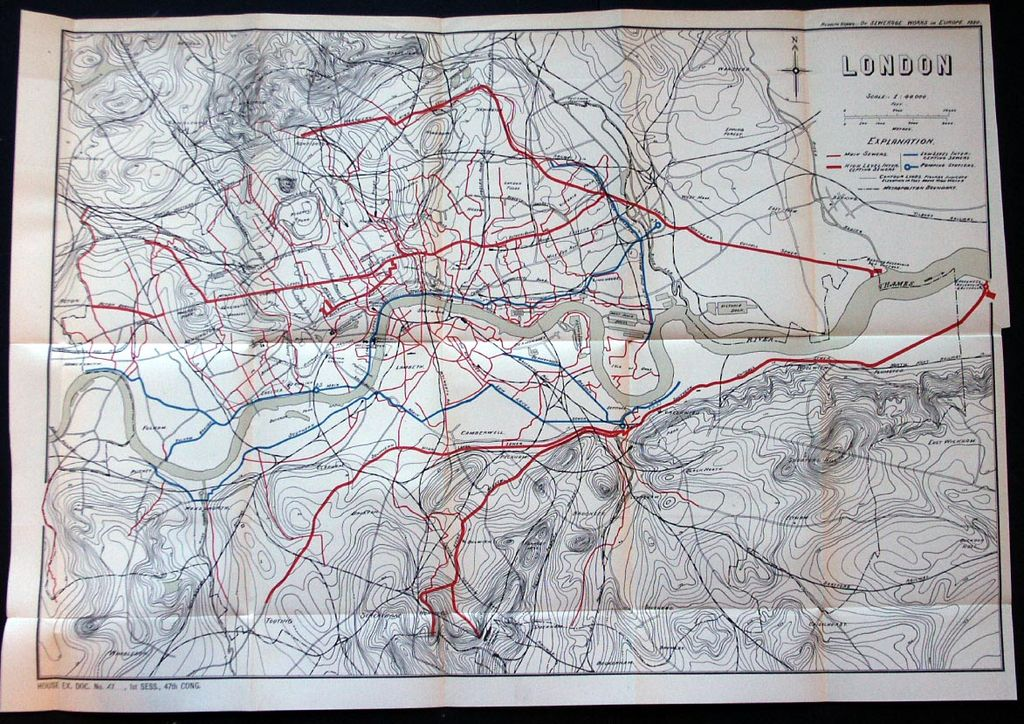
\includegraphics[width=1\textwidth]{2-cap1/complementos/mapas/1882-bazalgette-sistemadeesgotolondrino.jpg}{\par \footnotesize \textbf{Fonte:} \url{https://commons.wikimedia.org/wiki/File:Hering_lon-sewer-det02_1882.jpg}. \par}
\label{fig:esgotoslondres1882} 
\end{sidewaysfigure}

Entre uma epidemia e outra, um pesquisador assistente da \textit{Metropolitan Comission of Sewers}, \textit{Joseph William Bazalgette}, foi nomeado em 1856 diretor do órgão que veio a sucedê-la, o \textit{Metropolitan Board of Works}, e lá ficou até 1889; neste cargo, Bazalgette viveu em julho e agosto de 1858 -- como todos os londrinos -- o \textit{Grande Fedor}, causado pela exacerbação, pelo calor da época, do cheiro dos excrementos humanos não tratados e dos efluentes industriais que então eram lançados diretamente no Tâmisa. No mesmo ano, Bazalgette conseguiu aprovar junto ao Parlamento a construção, em Londres, de 132km de largas manilhas e canais em pedra para interceptar o afluxo de esgoto, e 1.800km de esgotamento de rua para captar os dejetos que, até então, fluiam livremente pelas ruas e vias públicas londrinas. Este fluxo de dejetos foi canalisado a jusante do Tâmisa, onde era despejado ainda sem tratamento. O plano de Bazalgette envolveu estações de bombeamento em \textit{Deptford Creek} e \textit{Crossness Point}, nos brejos de \textit{Erith}, todos no lado sul do Tâmisa; em \textit{Abbey Mills}, no vale do rio \textit{Lea}; e no aterro de \textit{Chelsea}, perto da ponte \textit{Grosvenor}, ao norte do Tâmisa \cite{bazalgette_london_1865, bazalgette_metropolitan_1865}. Embora Bazalgette fosse também adepto da teoria miasmática e pensasse, muito sinceramente, que a enorme obra sanitária que dirigiu serviria para acabar com os ``maus odores'' e, consequentemente, com as doenças epidêmicas, seus esforços tiveram sucesso, de fato, mas por um curioso efeito adverso: alargar a rede de esgotamento sanitário domiciliar e a drenagem pluvial significava conter, isolar e afastar do meio humano o bacilo do cólera, malgrado os miasmáticos duvidarem de sua existência.

\begin{figure}
\centering
\caption{Rambuteau e Haussmann, pioneiros do urbanismo e do planejamento urbano na França.}
\begin{footnotesize}
	\begin{subfigure}[b]{0.4\linewidth}
		\centering
		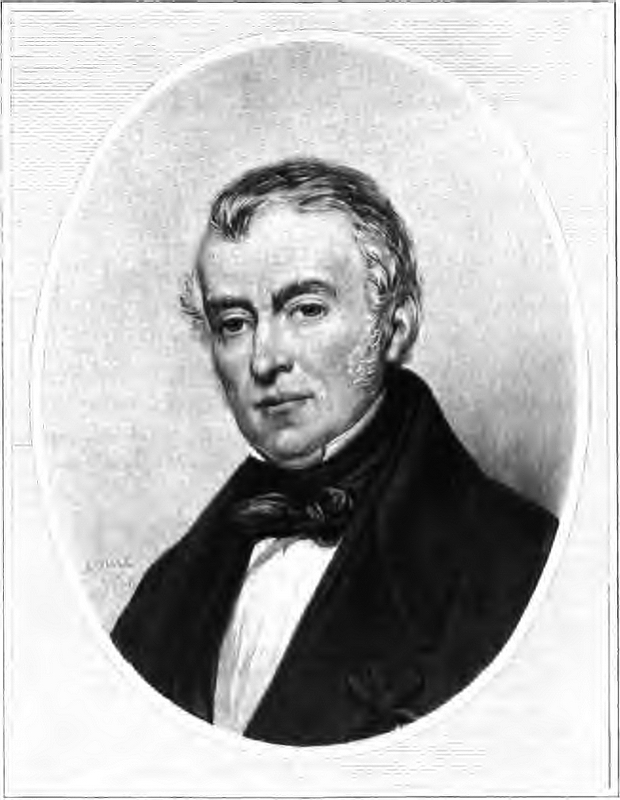
\includegraphics[width=1\textwidth]{2-cap1/complementos/fotos/Rambuteau.jpg} 
		\caption{Claude-Philibert Barthelot, conde de Rambuteau. \textbf{Fonte:} \url{https://commons.wikimedia.org/wiki/File:Le_comte_de_Rambuteau,d'après_Court,_1838_MMCR.jpg}.}
		\label{fig:rambuteau}
	\end{subfigure}	
	\
	\begin{subfigure}[b]{0.4\linewidth}
		\centering
		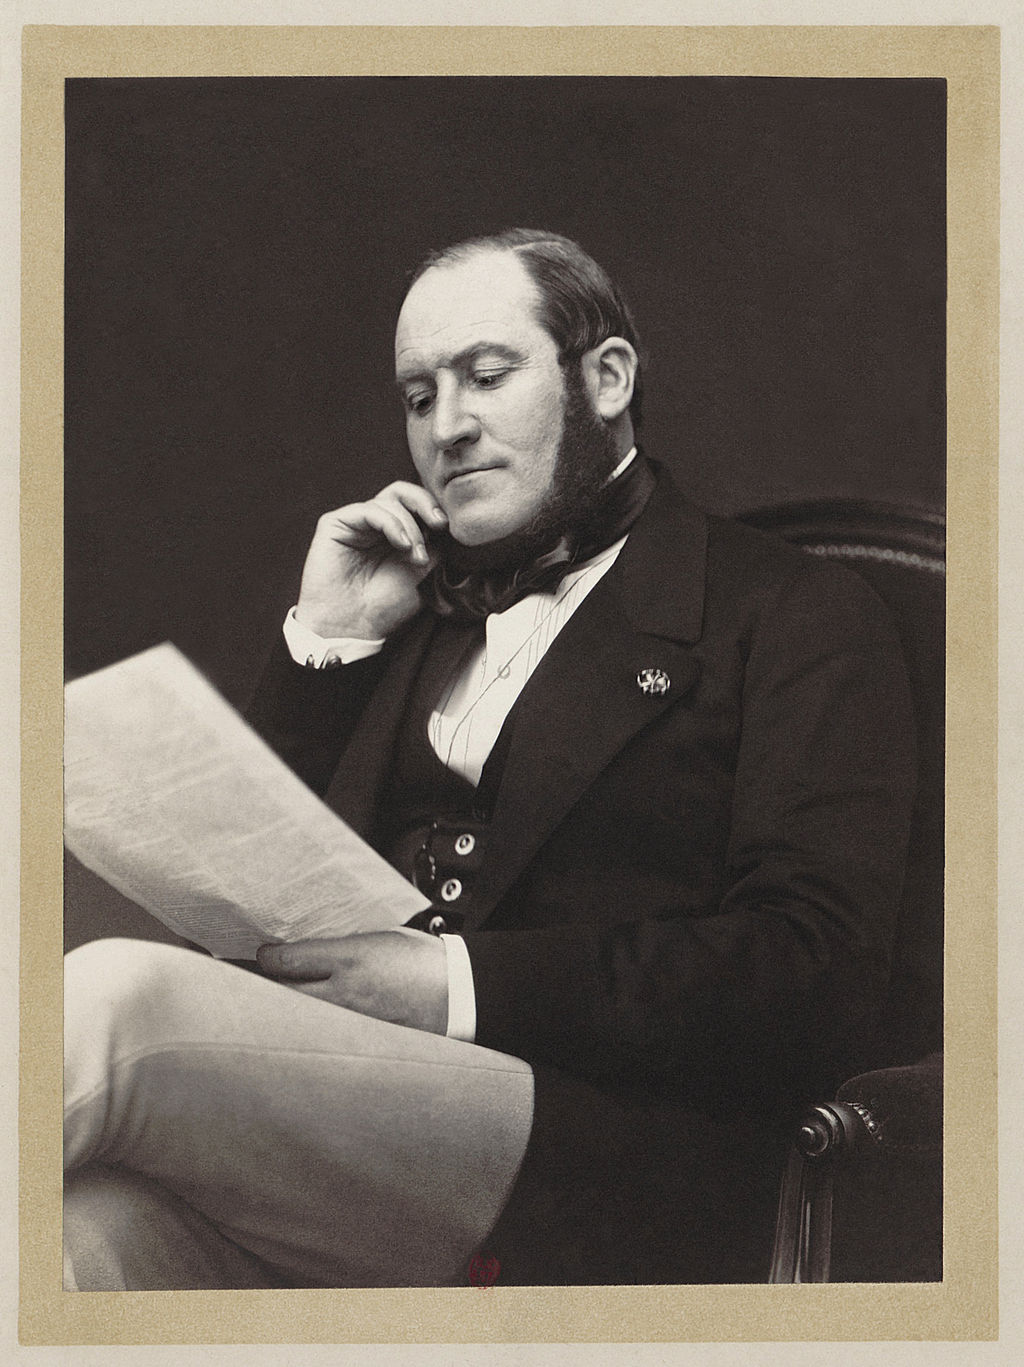
\includegraphics[width=1\textwidth]{2-cap1/complementos/fotos/haussmann.jpg}  
		\caption{Georges Eugène Haussmann. \textbf{Fonte:} \url{https://commons.wikimedia.org/wiki/File:Haussmann_BNF_Gallica.jpg}.}
		\label{fig:haussmann}
	\end{subfigure}	
\end{footnotesize}
\end{figure}

Vejamos agora a correlação entre teoria miasmática e obras públicas em \textit{Paris}. A ideia de realizar profundas reformas no centro de Paris era tão antigo e recorrente, sob diferentes formatos e nomes, que antecedeu ao \index{Georges-Eugène Haussmann}\index{Haussmann|seealso{Georges-Eugène Haussmann}}Haussmann prefeito, e que poderia, inclusive, ter sido feito inclusive sem ele. A cidade, quando de sua epidemia de cólera em 1832, havia crescido rumo aos \textit{faubourgs} em torno dos bulevares de Luís XIV, construídos em substituição às suas antigas muralhas; o centro mantinha as características medievais (principalmente as ruas estreitas e a malha viária irregular) e era dominado por uma encarniçada classe de proprietários, ciosa de seus direitos e pronta a defendê-los em qualquer instância onde se fizesse necessário \cite{faure_paris_2004}. Em 1833 \textit{Claude-Philibert Barthelot, conde de Rambuteau} foi posto à frente da prefeitura do Sena, onde permaneceu até 1848. Considerou ser seu dever ``dar aos parisienses água, ar e sombra'' \cite[p.~269]{rambuteau1905memoires}, comprimidos que eram pelas ruas estreitas e apertadas da cidade medieval; Rambuteau via-se no Hôtel de Ville como um ``comandante numa cidadela'' \cite[p.~269]{rambuteau1905memoires}, e assim tentou agir. A epidemia de cólera que assolou Paris em 1832 serviu a Rambuteau para dar início a um programa de melhoramentos urbanos iniciados com a abertura da \textit{Rue de Chanvreire} (atual \textit{Rue Rambuteau}), em 1834, com largura de 13 metros (incomum para os padrões da época), ligando o \textit{Marais} a \textit{Les Halles}; foi também aberta a \textit{Rue d'Arcole}, que atravessava a \textit{Île de la Cité} desde o arco da catedral de \textit{Notre-Dame} até o \textit{Hôtel de Ville} (ambos reformados, e o último ampliado, durante a gestão de Rambuteau); outras 112 ruas foram abertas. Seguiu-se a generalização da iluminação a gás em Paris, deixando Rambuteau ao sair de seu cargo 8.600 lampiões instalados; a rede de esgoto parisiense foi modernizada; novas pontes sobre o Sena foram construídas, sendo as mais famosas as de \textit{Bercy}, \textit{Saint-Pères} e Luís Felipe; a ilha de \textit{Louviers} foi anexada à margem direita do Sena por meio de um aterro. Rambuteau, ainda perseguindo seu programa de ``água, ar e sombra'', mandou plantar milhares de árvores e podar as já existentes; supervisionou a proliferação das ruas convexas, separadas das calçadas por sarjetas de escoamento, em substituição às antigas ruas côncavas em que as águas servidas acumulavam-se em poças; trouxe a Paris a pavimentação asfáltica, inicialmente ao redor do \textit{Palais-Royal}; ordenou a perfuração de poços em \textit{Grenele} e a instalação de duas mil fontes públicas com água encanada; a nota cômica deste processo de renovação urbana é o fato de os mictórios públicos instalados espaçadamente nos logradouros neste período terem sido apelidados de \textit{rambuteaux} em sua ``homenagem'' (\citeauthor{combeau_paris_2011}, \citeyear{combeau_paris_2011}, pp.~71-73; \citeauthor{rambuteau1905memoires}, \citeyear{rambuteau1905memoires}, pp.~325-399; \citeauthor{petti_eurfranba_2011}, \citeyear{petti_eurfranba_2011}, pp.~73-74). Em sua própria opinião, o conde de Rambuteau não pensa ter falhado em sua tarefa, pois teria feito o possível dentro das limitações legais e, no fim das contas, deixou a prefeitura do Sena sem dívidas \cite[p.~399]{rambuteau1905memoires}. 

O programa higienista concretizado primeiramente sob a gestão de Rambuteau foi retomado em escala monumental entre 1853 e 1870 por \index{Georges-Eugène Haussmann}\index{Haussmann|seealso{Georges-Eugène Haussmann}}\textit{Georges Eugène Haussmann} em seu mandato à frente da prefeitura do Sena. Recentes descobertas arquivísticas demonstram que a participação de \index{Georges-Eugène Haussmann}\index{Haussmann|seealso{Georges-Eugène Haussmann}}Haussmann na concepção geral das reformas no centro de Paris, ao contrário do que ele dá a entender em suas memórias (\citeauthor{haussmann1890memoires-1}, \citeyear{haussmann1890memoires-1}, \citeyear{haussmann1890memoires-2}, \citeyear{haussmann1890memoires-3}), foi menor do que se pensa: a \textit{Commission des embellissements de Paris}, nomeada diretamente por Napoleão III, composta por topógrafos, engenheiros e profissionais correlatos (como \textit{Théodore Jacoubet}, \textit{Hippolyte Meynadier} e os irmãos \textit{Louis} e \textit{Félix Lazaire}), reuniu-se pela primeira vez em 16 de agosto de 1853 e trabalhou até que seu diretor, \textit{Henri Siméon}, entregou ao imperador em 27 de dezembro de 1853 um plano bastante completo das modificações a serem feitas em Paris; muitas delas foram discutidas entre Napoleão III e a \textit{Comission} sem que \index{Georges-Eugène Haussmann}\index{Haussmann|seealso{Georges-Eugène Haussmann}}Haussmann sequer tomasse parte; foi o plano resultante dos trabalhos da \textit{Comission}, com algumas alterações, que \index{Georges-Eugène Haussmann}\index{Haussmann|seealso{Georges-Eugène Haussmann}}Haussmann implementou durante sua gestão à frente da prefeitura do Sena, depois de haver pedido -- e conseguido -- a extinção da comissão \cite{bourillon_changer_1999,casselle_embel_1997}\footnote{O artigo pioneiro de \citeonline{casselle_embel_1997}, quem primeiro divulgou a existência deste plano, chega a comparar, uma a uma, todas as obras propostas pela \textit{Comission} com aquelas realizadas por \index{Georges-Eugène Haussmann}\index{Haussmann|seealso{Georges-Eugène Haussmann}}Haussmann ou por seus sucessores. Observa, adicionalmente, que a cidade inteira foi coberta pelo projeto original (enquanto \index{Georges-Eugène Haussmann}\index{Haussmann|seealso{Georges-Eugène Haussmann}}Haussmann trabalhou principalmente na sua parte oeste), e que a malha viária dos antigos subúrbios anexados em 1860 estava, também, já desenhada no plano da \textit{Comission} de 1853, como a indicar um plano concebido de antemão.}. Quer como mentor intelectual, quer como gestor a mão-de-ferro de planos pré-concebidos, as obras regidas por \index{Georges-Eugène Haussmann}\index{Haussmann|seealso{Georges-Eugène Haussmann}}Haussmann, ao contrário daquelas regidas por Rambuteau, são muito maiores em escala e número, e muito mais conhecidas e comentadas \cite{bourillon_changer_1999, casselle_embel_1997, dansette_haussmann_1972, faure_paris_2004, hourticq_haussmann_1971, petti_eurfranba_2011, pinkney_ordevpar_1955, pinkney_paris_1957, vossen_villes_1947}, sendo desnecessário para o objeto desta pesquisa detalhá-las neste momento; cabe, muito mais, ressaltar que \index{Georges-Eugène Haussmann}\index{Haussmann|seealso{Georges-Eugène Haussmann}}Haussmann era outro adepto da teoria miasmática (\citeauthor{haussmann1890memoires-2}, \citeyear{haussmann1890memoires-2}, p.~318; \citeyear{haussmann1890memoires-3}, p.~421), e que a orientação geral das intervenções urbanas regidas por seus planos seguia, mesmo que não intencionalmente, o programa de Rambuteau e de outros predecessores (Chabrol, Berger, o ``plano dos artistas'', os largos \textit{boulevards} à moda de Luís XIV etc.). Num só e grande resumo:

\begin{citacao}
Mas, afinal, o que é haussmannização? Através dos escritos de \index{Georges-Eugène Haussmann}\index{Haussmann|seealso{Georges-Eugène Haussmann}}Haussmann, não se pode chegar a um conceito preciso, uma vez que ele não propõe uma doutrina ou uma teoria de melhorias urbanas.
[\dots] O próprio \index{Georges-Eugène Haussmann}\index{Haussmann|seealso{Georges-Eugène Haussmann}}Haussmann chama seu trabalho de regularização, que não pretende uma universalidade científica, não se baseia numa crítica social, nem propõe um modelo espacial.
[\dots] As intervenções haussmannianas mudam a maneira de pensar a cidade, tomando como principal elemento a rua e criando uma rede viária composta por um tecido arquitetônico que destrói bairros insalubres e vielas. Expulsam a população residente, melhoram a higiene e a circulação, mudam a imagem da área central, e a cidade prepara-se para um novo modo de vida. A rua do século XIX destrói e modifica a rua medieval. A caixa da rua aumenta, as fachadas são reconstruídas, os trechos irregulares são substituídos por outros com desenho regular, geométrico e reto. Diferentes dos bulevares de Luís XIV -- projetados no lugar das antigas muralhas, locais para o desfrute e o passeio --, os bulevares do século XIX, de \index{Georges-Eugène Haussmann}\index{Haussmann|seealso{Georges-Eugène Haussmann}}Haussmann, são artérias criadas para a circulação rápida, o tráfego pesado. O espaço haussmanniano é o espaço público -- a rua, o passeio, as praças --, o espaço da mobilidade. A originalidade desse projeto está no conceito de sistema de circulação e de respiração, que superpõe malhas hierarquizadas, pertencentes a uma rede em estrela. Esse desenho não resulta num espaço homogêneo, uma vez que se acentua a divisão social entre leste e oeste, entre periferia e centro, mas ainda não se adota a ideia de cidade por setores. A hierarquia do sistema de comunicações muda a ordem de valores.
[\dots] Na cidade haussmanniana, é introduzida uma nova forma de construção da paisagem urbana. As intervenções no núcleo central tratam o conjunto dos espaços heterogêneos como uma entidade única e o dotam de isotropia. Constrói-se uma imagem urbana mais coerente, com um tipo de arquitetura definida, em que o imóvel se integra no espaço público através de uma projetação regulamentada \cite[pp.~68,~77]{petti_eurfranba_2011}.
\end{citacao}

A saúde pública e o bem-estar dos cidadãos parisienses era o principal argumento para a instalação, reforma ou ampliação de infraestruturas sanitárias e equipamentos coletivos, mas não era possível esconder os profundos arranjos financeiros necessários a tais reformas: a oposição parlamentar a Napoleão III atacou \index{Georges-Eugène Haussmann}\index{Haussmann|seealso{Georges-Eugène Haussmann}}Haussmann incessantemente pela falta de transparência nos gastos, especialmente com o escândalo das transações escusas envolvendo o \textit{Crédit Foncier}, a \textit{Caisse des Travaux de Paris} e a firma \textit{Ardoin, Ricardo et Cie.} \cite{pinkney_paris_1957}. Houve desde o início das intervenções resistência encarniçada ao programa de reformas também entre proprietários, que julgavam indevidas as expropriações e as intervenções sobre suas propriedades \cite{paccoud_hauspropr_2012}. A força combinada destas pressões políticas levou Napoleão III a retirar o apoio a \index{Georges-Eugène Haussmann}\index{Haussmann|seealso{Georges-Eugène Haussmann}}Haussmann, que saiu da prefeitura do Sena em 1870. Não obstante, as reformas ditas ``haussmannianas'' (mais bem descritas como \textit{reformas do Segundo Império}), numa Paris cujo centro estava sendo progressivamente abandonado pelas classes abastadas e ocupado pelos trabalhadores e pelos miseráveis, cujos alugueis abasteciam os bolsos dos proprietários fundiários, teria beneficiado exatamente os mais abastados, já em vias de instalação nos \textit{faubourgs} e subúrbios parisienses, a obter vantagens na luta encarniçada pela retomada do centro de Paris \cite{faure_paris_2004}.

\begin{figure}[!htp]
\centering
\caption{Duas obras do período de Georges Eugène Haussmann à frente da prefeitura do Sena.}
\begin{subfigure}{0.9\textwidth}
\centering
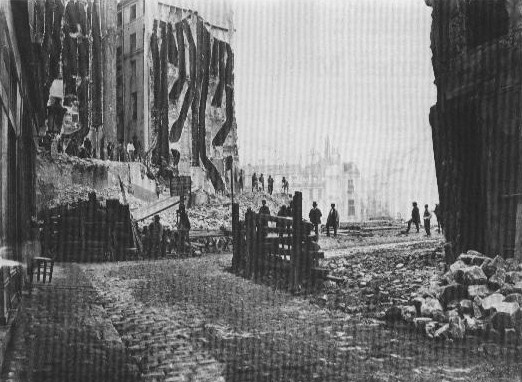
\includegraphics[width=1\textwidth]{2-cap1/complementos/fotos/Percement_avenue_de_lOpera.jpg}{\par \footnotesize Abertura da \textit{Avenue de l'Ópera}. \textbf{Fonte:} \url{https://commons.wikimedia.org/wiki/File:Percement_avenue_de_l'Opéra.jpg}.}
\label{fig:aberturaopera}
\end{subfigure}
\
\begin{subfigure}{0.9\textwidth}
\centering
\includegraphics[width=1\textwidth]{2-cap1/complementos/fotos/rivoli.jpg}{\par \footnotesize Construção noturna da \textit{Rue de Rivoli}\textbf{Fonte:} \url{https://commons.wikimedia.org/wiki/File:Travaux_nocturnes_des_constructions_de_la_rue_de_Rivoli,_éclairés_par_la_lumière_électrique.jpg}. }
\label{fig:obrasrivoli}
\end{subfigure}
\end{figure}

A análise de exemplos poderia incluir a construção em Viena (Áustria) da \textit{Ringstrasse} e seus prédios monumentais por ordem do imperador Francisco José I (1857-1913) \cite{abercrombie_vienna_1910,abercrombie_vienna_1911,aman_vienna_1911}; poderia incluir o ``embelezamento'' de Bruxelas (Bélgica) sob a regência do burgomestre \textit{Jules Anspach} e do rei \textit{Leopoldo II} (\textit{le roi bâtisseur}, ``o rei construtor''), em especial o tamponamento e canalização do Sena entre 1859 e 1873 \cite{abercrombie_brussels1_1912,abercrombie_brussels2_1912,abercrombie_brussels3_1913}; poderia avançar pela expansão de Barcelona de acordo com o plano pioneiro de \textit{Ildefonso Cerdà} (1860) \cite{aibarbijker_barcelona_1997,ciervo_cerda_1976,soriaypuig_cerda_1995,wynn_barcelona_1979}; poderia seguir pelo \textit{Risanamento} de Florença (1865-1895), Nápoles (1885-1904) e outras cidades italianas em seguida à \textit{Unificazione} \cite{biocca_naples_1992,parisi_napoli_2001,piccinato_igiene_1989,rossi_napoli_2011}\dots Há um longo fio condutor a ligar o higienismo dos primeiro e segundo terços do século XIX ao ``proto-urbanismo'' do último terço deste mesmo século e ao urbanismo do primeiro terço do seguinte -- se é que há, realmente, alguma solução de continuidade, salvo pela escala e escopo das intervenções propostas em ambos os casos. 

\begin{a3paisagem}
\begin{figure}[!htp]
\caption{Planta de situação da capital e da cidade residencial de Berlim e seus arredores -- plano de desenvolvimento dos arredores de Berlim (1856).}
\centering
\includegraphics[height=0.9\textheight]{2-cap1/complementos/mapas/1856_Bauplanungen.jpg}{\par \footnotesize \textbf{Fonte:} \url{https://commons.wikimedia.org/wiki/File:1856_Bauplanungen.jpg}.}
\label{fig:bauplannungen1856} 
\end{figure}
\end{a3paisagem}

\begin{a3paisagem}
\begin{figure}[!htp]
\caption{Plano para Berlim e arredores até Charlottenburg (1862), desenhado por Ferdinand Boehm.}
\centering
\includegraphics[height=0.9\textheight]{2-cap1/complementos/mapas/Boehm_Berlin_1862.jpg}{\par \footnotesize \textbf{Fonte:} \url{http://nbn-resolving.de/urn:nbn:de:kobv:109-opus-104224}. Os 14 departamentos do \textit{plano Hobrecht} estão rotulados como algarismos romanos. Os assentamentos programados estão indicados por letras maiúsculas e ruas por meio de algarismos arábicos, cada um dentro de um departamento de planejamento.}
\label{fig:berlin1862} 
\end{figure}
\end{a3paisagem}

\begin{a3paisagem}
\begin{figure}[!htp]
\caption{Plano de Giuseppe Poggi para Florença (1865).}
\centering
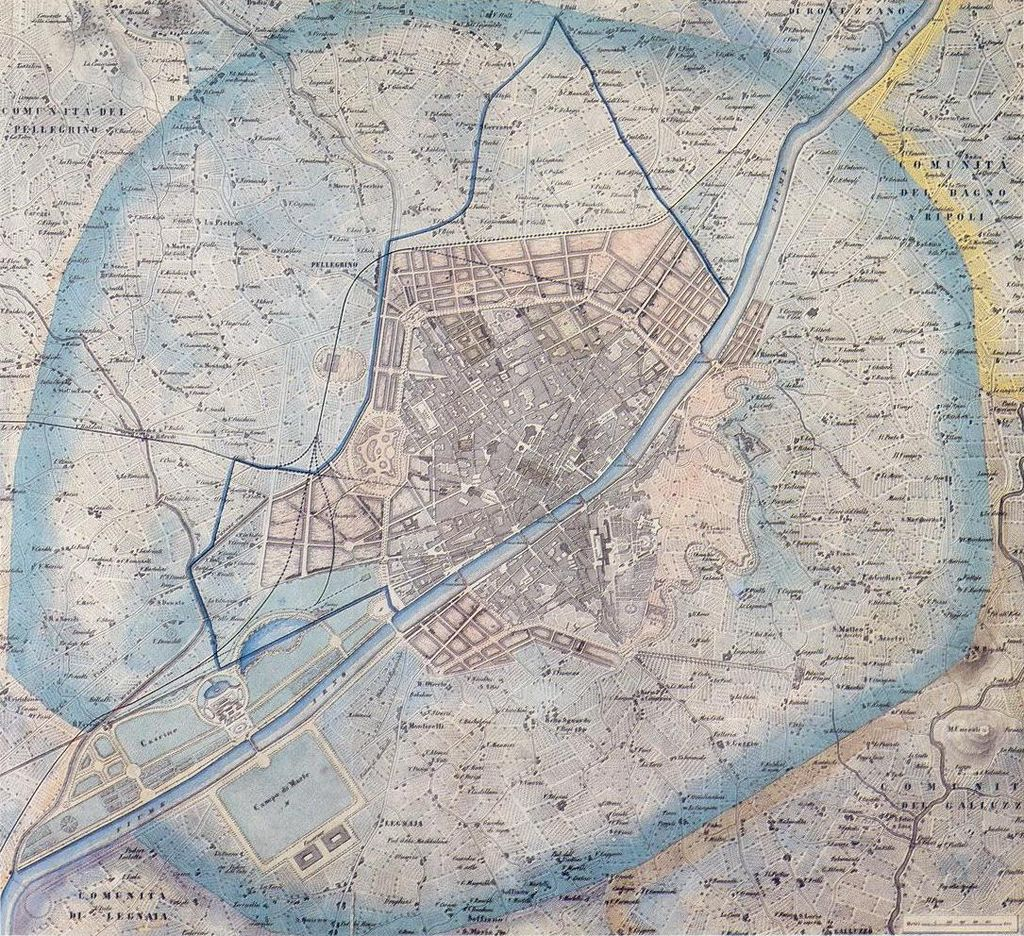
\includegraphics[height=0.9\textheight]{2-cap1/complementos/mapas/1865-planopoggi-florenca.jpg}{\par \footnotesize \textbf{Fonte:} \url{https://commons.wikimedia.org/wiki/File:Piano_Poggi_(Firenze,_1865)_-_1.JPG}.}
\label{fig:florenca1865} 
\end{figure}
\end{a3paisagem}

\begin{a3paisagem}
\begin{figure}[!htp]
\caption{Plano da cidade de Heilbronn, por Reinhardt Baumeister (1879).}
\centering
\includegraphics[height=0.9\textheight]{2-cap1/complementos/mapas/heilbronn.jpg}{\par \footnotesize \textbf{Fonte:} \url{https://commons.wikimedia.org/wiki/File:Stadtbauplan_Heilbronns_von_1879_auf_der_Grundlage_des_Generalbebauungsplanes_von_Reinhard_Baumeister.jpg}. }
\label{fig:heilbronn1879} 
\end{figure}
\end{a3paisagem}

Para os fins desta pesquisa, entretanto, os dois casos paradigmáticos apresentados já demonstram, sem necessidade de análise detalhada de outros exemplos, que o alvo preferencial das políticas do higienismo no século XIX foram os \textit{centros urbanos ditos ``degradados''} e as \textit{construções insalubres}. Ora, mas \textit{quem morava em tais construções e centros era exatamente quem não tinha condições de pagar para morar em imóveis em condições mais higiênicas}; ``higienizar'', ``embelezar'', fazer ``melhoramentos'' implicou, na maioria dos casos, em \textit{processos maciços de remoção dos trabalhadores e dos mais pobres dos bairros centrais}\footnote{No caso francês, \citeonline[p.~445]{faure_paris_2004} registra que ``dos 102 imóveis construidos nos anos 1860 pela companhia imobiliária dos irmãos Péreire, no atual bulevar Voltaire -- ou seja, num \textit{faubourg} do leste de Paris -- apenas 19\% dos apartamentos, dado o valor dos alugueis, parecem, a rigor, acessíveis a famílias operárias, a menos que se trate de cubículos nos sótãos''. Diz ainda que ``as operações de 1849-1853 tiveram como efeito desalojar 9.081 'trabalhadores' [\dots]: 2,1\% partiram para os \textit{banlieues}, e a imensa maioria dos outros se distribuiriam nos \textit{faubourgs}, uma reduzida minoria tendo permanecido nos bairros do centro, esperando, sem dúvida, que a continuação das obras não lhes desse caça'' (\Ibidem[p.~445]{faure_paris_2004}). No caso napolitano, tanto antes quanto depois do \textit{Risanamento} \citeonline{serao1906ventre} denunciou o caráter deletério das condições de vida dos trabalhadores mais pobres. No caso vienense, a \textit{Ringstrasse} acentuou a segregação socioespacial já existente, separando os burgueses da nova e resplandescente avenida, os operários dos subúrbios industriais como \textit{Ottakring} e uma pequena burguesia saudosa da antiga cidade \cite[p.~26]{maderthanermuser_vienna_2003}.}. O longo experimento higienista do século XIX interferiu também sobre a moradia, em especial sobre a moradia dos trabalhadores. A \textit{habitação operária} tornou-se, em paralelo à questão sanitária, pauta importante para os gestores públicos e os encontros internacionais de arquitetos e engenheiros: infiltou-se no Congresso Internacional de Higiene de 1878 em Paris \cite{congres_hygiene_1878}, fato repetido nos congressos internacionais de arquitetos de Londres (1908) e Viena (1910) \cite{QUINTOJR1990}, e mereceu um congresso internacional voltado apenas ao seu debate \cite{fleming_housing_1897}. Em nenhum deles, entretanto, chegou-se a qualquer solução definitiva quanto à questão, restringindo-se tais encontros ao relato das experiências locais em habitação operária e a soluções tópicas\footnote{Veja-se, como exemplo, o voto final da sessão plenária de 7 de agosto do Congresso Internacional de Higiene de 1878: depois de longos relatos e debates sobre a habitação dos operários em Paris, Londres, Bruxelas e outras metrópoles europeias, os presentes concordaram numa única recomendação: reforçar a legislação urbanística existente e transformar em exigência legal a instalação de água nas casas para operários \cite[p.~597]{congres_hygiene_1878}.}.

Tudo indica, até o momento, que os conflitos sociais são elemento essencial da produção, apropriação e uso dos territórios urbanos no período. Mas se há conflito social neste âmbito, seria a estética arquitetônica, ela própria, também produto dos conflitos sociais de seu tempo? Ou estaria imune a tal influência?

\subsubsection{As artes de morar: ecletismo e pré-modernismos, por dentro e por fora}\label{subsec:armor}

Entre os estilos arquitetônicos dezenovistas, o que mais interessa a esta pesquisa, pelo que se pôde encontrar nos documentos consultados, é como que um ``não-estilo'': o \textit{eclético}, resumidamente conceituado por um especialista como

\begin{citacao}
a cultura arquitetônica própria de uma classe burguesa que dava primazia ao conforto, amava o progresso (especialmente quando melhorava suas condições de vida), amava as novidades, mas rebaixava a produção artística e arquitetônica ao nível da moda e do gosto \cite[p.~13]{patetta_ecletismo_1987}.
\end{citacao}

A própria etimologia grega da palavra -- o adjetivo \textgreek{ἐκλεκτικός}, \textit{eklektikos}, ``escolhido entre os melhores'', por sua vez derivado de \textgreek{ἐκλεκτός}, \textit{eklektos}, ``escolhido, seleto'' -- indica uma de suas características principais: a escolha pelo arquiteto ou por seus clientes, na tradição arquitetônica passada, de elementos ora coerentes, ora díspares, que compusessem a obra de acordo com o gosto do freguês ou com a função a ser dada ao imóvel. Justo por isto, há enorme heterogeneidade estilística no campo eclético, sendo bastante difícil encontrar elementos comuns que não as justaposições e os revivalismos. 

Como movimento artístico, o ecletismo ocorre na arquitetura e na arte do século XIX. As primeiras vanguardas desse movimento datam da terceira década do século XIX com a afirmação de pulsões neo-góticas em áreas francófonas e neo-renascentistas em Florença. Por volta de 1840, na França, em reação à hegemonia do estilo greco-romano, os arquitetos começam a propor a retomada de outros modelos históricos como, por exemplo, o gótico e o românico. O principal teórico do ecletismo arquitetônico é o francês \textit{César Denis Daly} (1811-1893) que o entende como ``o uso livre do passado''. Não se trata de uma atitude de simples copista, mas da habilidade de combinar as características superiores desses estilos em construções que satisfaçam a demandas da época por todo tipo de edificação. Na segunda metade do século XIX, o ecletismo tem forte presença na Europa. O estilo \textit{Segundo Império} ou \textit{Napoleão III} é caracterizado pela realização de importantes edifícios ecléticos, como o Teatro Ópera de Paris, projetado por \textit{Charles Garnier} (1825-1898).

\begin{figure}[!htp]
\centering
\caption{\textit{Hôtel privé} de primeira classe no estilo Segundo Império/Napoleão III.}
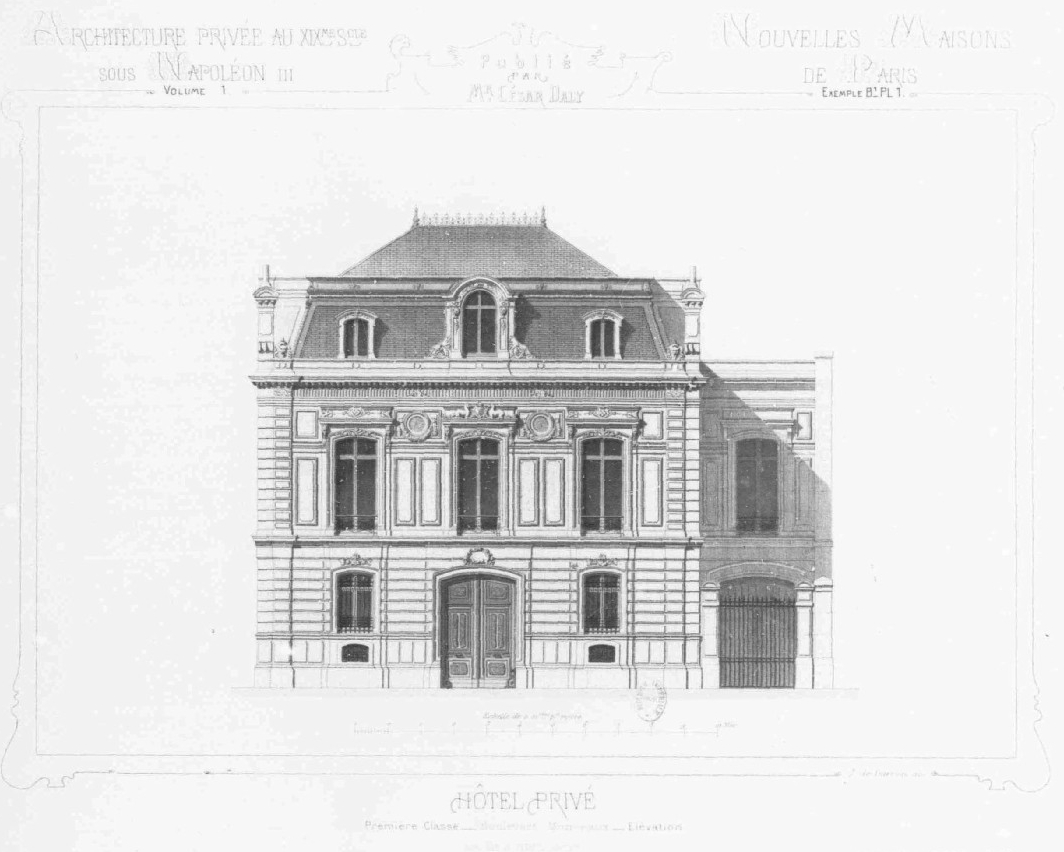
\includegraphics[width=1\textwidth]{2-cap1/complementos/fotos/daly01-0.JPEG}{\par \footnotesize \textbf{Fonte:} \textbf{L’architecture privée au XIXe siècle, sous Napoléon III:} nouvelles maisons de paris et des environs, de César Denis \citeonline{daly_architecture1_1864}. \par}
\label{fig:hotelprimclas} 
\end{figure}

\begin{figure}[!htp]
\centering
\caption{\textit{Hôtel privé} de segunda classe no estilo Segundo Império/Napoleão III.} 
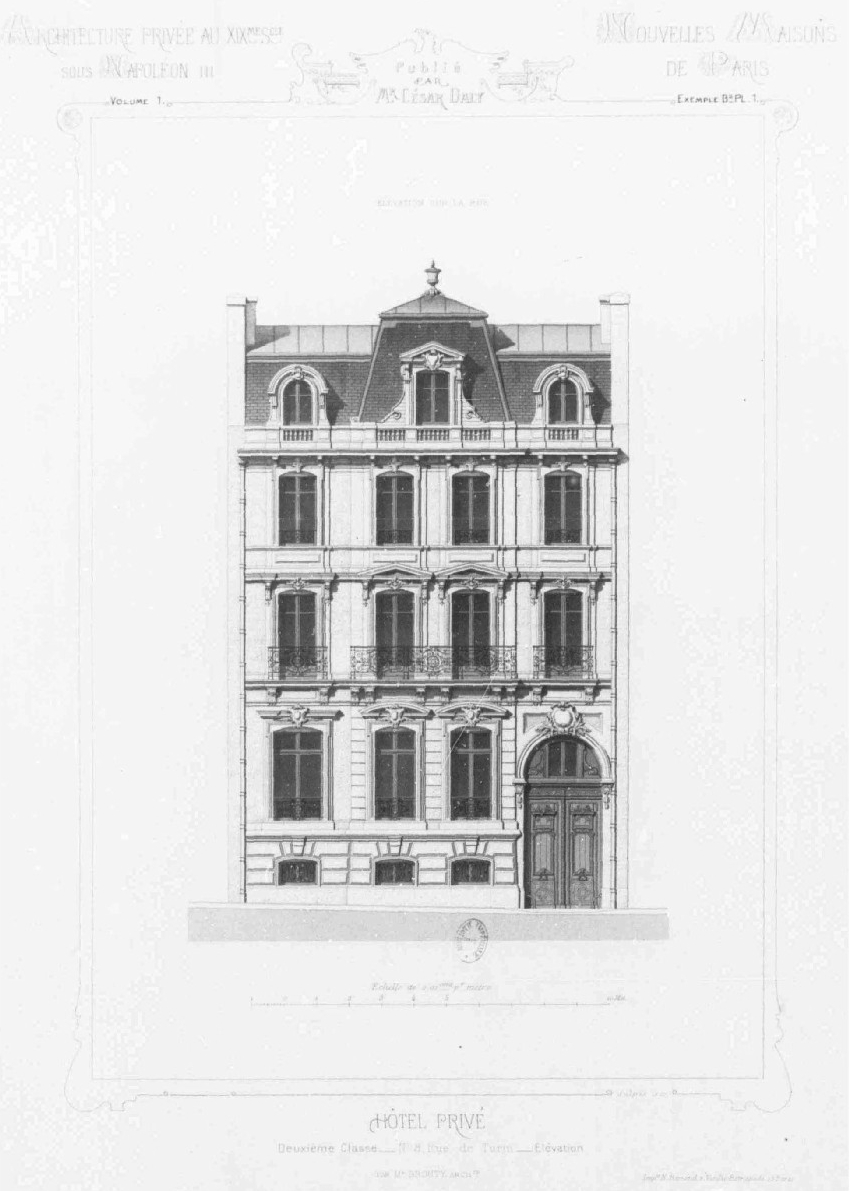
\includegraphics[width=1\textwidth]{2-cap1/complementos/fotos/daly01-1.JPEG}{\par \footnotesize \textbf{Fonte:} \textbf{L’architecture privée au XIXe siècle, sous Napoléon III:} nouvelles maisons de paris et des environs, de César Denis \citeonline{daly_architecture3_1864}. \par}
\label{fig:hotelsegclas} 
\end{figure}

\begin{figure}[!htp]
\centering
\caption{\textit{Villa suburbaine} de primeira classe no estilo Segundo Império/Napoleão III.}
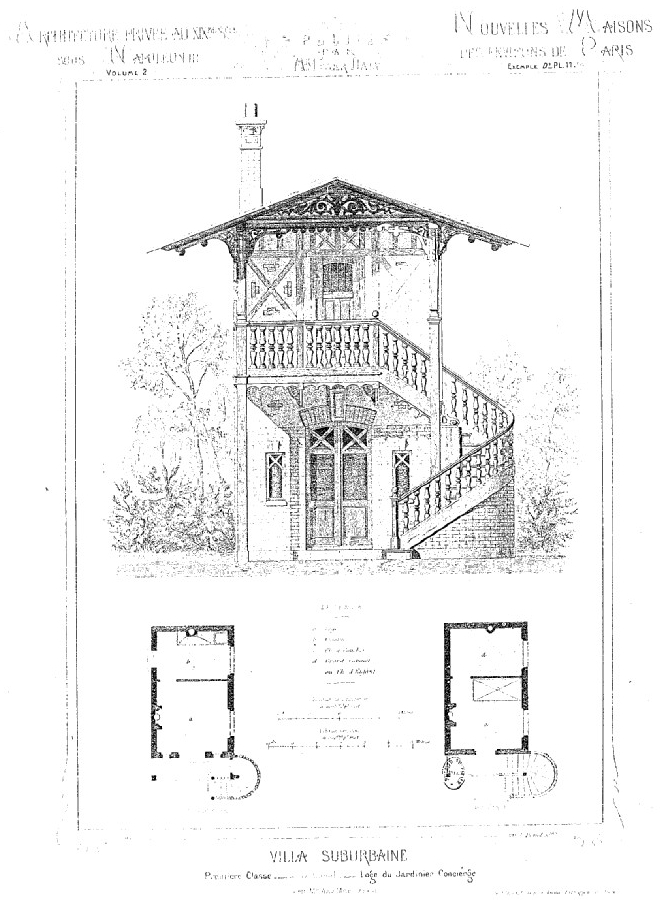
\includegraphics[width=1\textwidth]{2-cap1/complementos/fotos/daly03-4.JPEG}{\par \footnotesize \textbf{Fonte:} \textbf{L’architecture privée au XIXe siècle, sous Napoléon III:} nouvelles maisons de paris et des environs, de César Denis \citeonline{daly_architecture3_1864}. \par}
\label{fig:villaprimclas} 
\end{figure}

\begin{figure}[!htp]
\centering
\caption{\textit{Villas suburbaines} de segunda classe no estilo Segundo Império/Napoleão III.}
\begin{subfigure}[b]{0.8\linewidth}
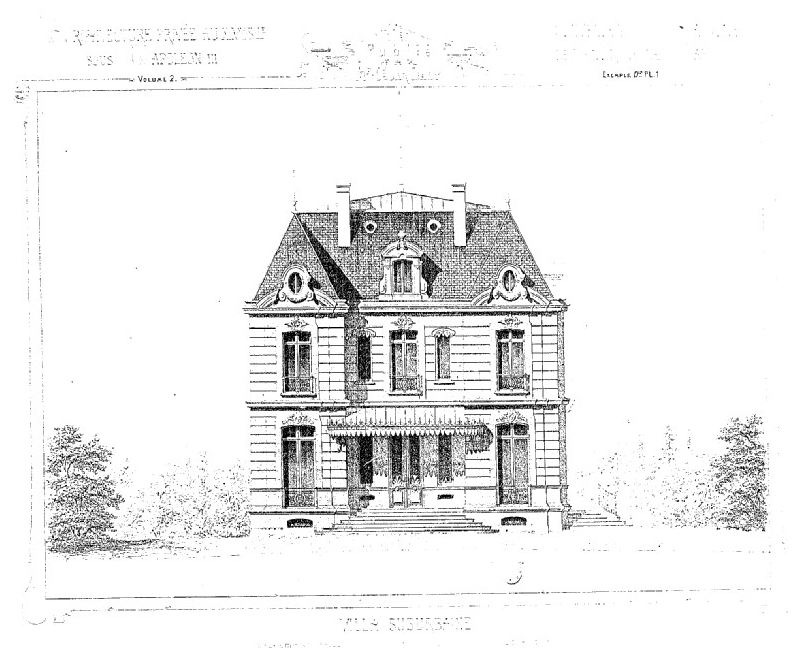
\includegraphics[width=0.9\textwidth]{2-cap1/complementos/fotos/daly03-5.JPEG}
\caption{\textbf{Fonte:} L’architecture privée au XIXe siècle, sous Napoléon III: nouvelles maisons de paris et des environs, de César Denis \citeonline{daly_architecture3_1864}.}
\label{fig:villasegclas1}
\end{subfigure}
\
\begin{subfigure}[b]{0.8\linewidth}
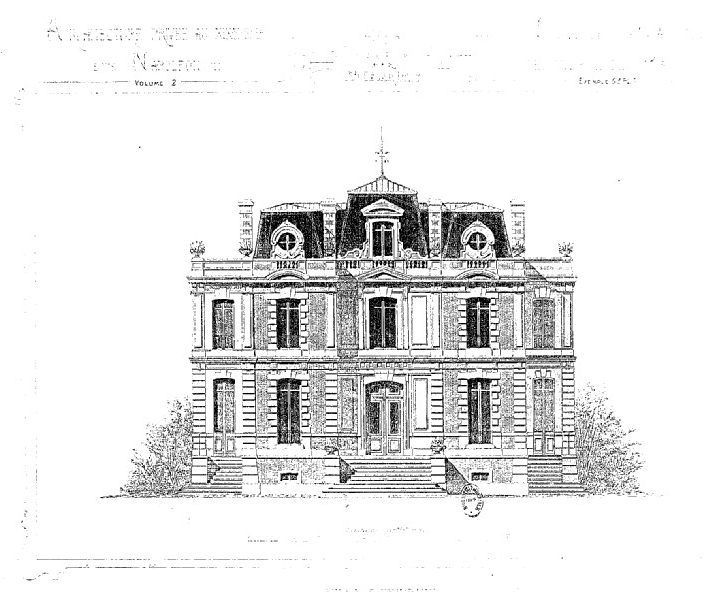
\includegraphics[width=0.9\textwidth]{2-cap1/complementos/fotos/daly03-6.JPEG}
\caption{\textbf{Fonte:} \textbf{L’architecture privée au XIXe siècle, sous Napoléon III:} nouvelles maisons de paris et des environs, de César Denis \citeonline{daly_architecture3_1864}.}
\label{fig:villasegclas2}
\end{subfigure}
\end{figure}

\begin{figure}[!htp]
\centering
\caption{\textit{Villa suburbaine} de terceira classe no estilo Segundo Império/Napoleão III.}
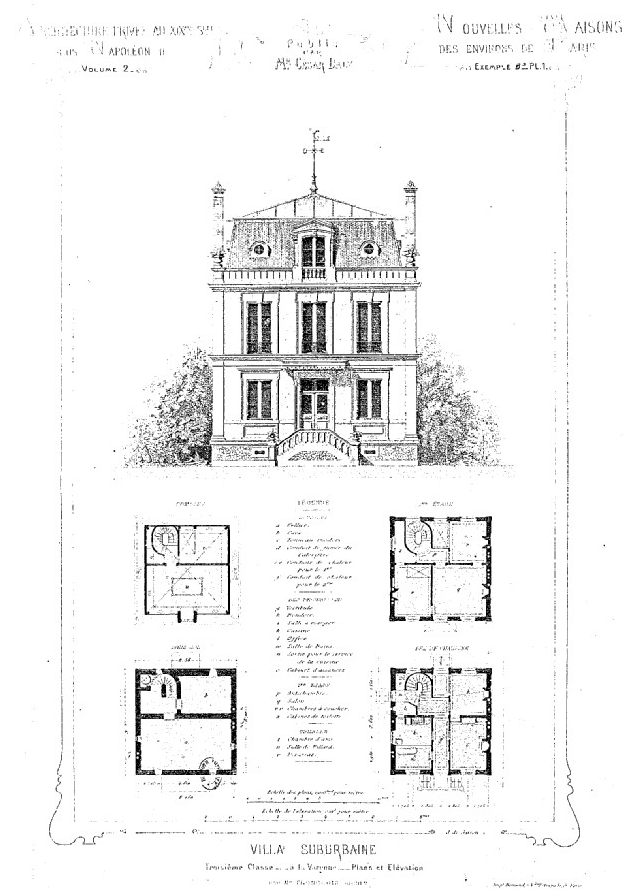
\includegraphics[width=1\textwidth]{2-cap1/complementos/fotos/daly03-8.JPEG}{\par \footnotesize \textbf{Fonte:} \textbf{L’architecture privée au XIXe siècle, sous Napoléon III:} nouvelles maisons de paris et des environs, de César Denis \citeonline{daly_architecture3_1864}. \par}
\label{fig:villaterclas} 
\end{figure}

As diferentes linguagens artísticas foram reelaboradas a critério do arquiteto seguindo a sua inspiração pessoal. No princípio a tendência eclética se impôs especialmente na realização de estruturas para festas e grandes eventos; sucessivamente, começou a ser apreciada também para mobiliar casas e jardins, nos quais, frequentemente e de forma totalmente acrítica, misturavam-se tempos gregos, vasos árabes e pavilhões indianos. Na época afirmou-se o costume de mobiliar cada sala das residências mais luxuosas segundo um estilo diferente. Assim, marceneiros e ebanistas, por exemplo, tiveram que aprender a lidar com formas bastante diferentes entre si. 

Mas foi o modernismo industrial do século XIX que serviu como trampolim para o sucesso do estilo eclético. Em 1851, pela primeira vez, na \textit{Great Exhibition} em Londres foram realizados pavilhões onde os mercadores das principais nações do mundo foram chamados para expor suas próprias obras. Percebeu-se que as empresas presentes exibiam para a atenção do publico obras que mostravam a história recente ou antiga da própria nação. Houve euforia em expor todas as obras antigas remodeladas, havendo-se, inicialmente, um certo grau de dependência relativamente aos modelos originais, quase como se fosse uma cópia, uma reprodução. A fantasia de cada artista, artesão, arquiteto, ourives, etc. não demorou para se afirmar, levando os artistas a formular obras personalizadas que ``condensavam'' vários séculos de história. Era isso o que os clientes queriam, curiosos por artes distantes e citações culturais magníficas mostrando que aquela geração iria reviver uma era áurea. Todas as grande técnicas do passado reviviam numa miríade de moveis, cerâmicas e
objetos do Ecletismo.

Grosso modo, as obras arquitetônicas em estilo eclético podem ser classificadas em três categorias principais, cujas características são assim definidas:

\begin{itemize}
\item A \textit{composição estilística}: caracteriza-se por um \textit{maior rigor filológico} e pela \textit{imitação precisa e coerente de um único e preciso estilo arquitetônico}. Os exemplos mais destacados são o \textit{neogrego}, o \textit{neo-egípcio} e o \textit{neogótico}.
\item O \textit{historicismo tipológico}: caracteriza-se por uma \textit{relação apriorística de cunho analógico entre estilo e função} através de valores associativos, não raro arbitrários. A arquitetura medieval, por exemplo, forneceu aos arquitetos os traços místicos e a religiosidade para as novas igrejas; na arquitetura renascentista foram encontradas as características áulicas elegantes para os edifícios públicos; na arquitetura barroca, ou nos estilos orientais, a festividade exigida pelos equipamentos; no classicismo pesado do coríntio romano, o caráter apropriado aos solenes edificios parlamentares, aos museus e aos ministérios.
\item Os \textit{pastiches compositivos}: caracterizam-se pela \textit{fusão de elementos arquitetônicos de estilos distintos, historicamente inadmissíveis}, sob cujos elementos díspares, não raro beirando o mau gosto, mascaravam-se muitas vezes soluções estruturais inovadoras \cite[p.~14-15]{patetta_ecletismo_1987}.
\end{itemize}

Quer seja ele o estilo ostentatório dos \textit{nouveaux riches} desprovidos da bagagem cultural do \textit{Ancièn Régime} e dispostos a demarcar seu espaço social por meio da sobreposição, às vezes sem nexo, das novas modas da Escola de Belas-Artes de Paris \cite[pp.~315-319]{guerrand_espacos_2009}, quer seja um estilo arquitetônico com méritos e conquistas próprios em processo de redescoberta desde pelo menos a metade dos anos 1970, a partir da crítica ao ideário arquitetônico do Modernismo que o sucedeu e criticou duramente \cite{almeida_victoria_1997, almeida_vitrinescomercio_2014, patetta_ecletismo_1987, puppi_hisnamod_1998}, interessa a esta pesquisa o fato de o ecletismo ser o estilo arquitetônico mais encontrado no distrito soteropolitano estudado, especialmente nas modalidades de \textit{historicismo tipológico} e \textit{pastiche compositivo}, com maior frequência esta última.

A América Latina foi terreno fértil para as experimentações arquitetônicas, especialmente as ecléticas, e isto por questões muito particulares. No final do século XIX, findos os processos independentistas, consolidadas as fronteiras nacionais e assentados os blocos hegemônicos na política após um século pontilhado por guerras, \textit{pronunciamientos} e rebeliões, as classes dominantes nos países latinoamericanos viram na arquitetura um meio de reafirmar sua identidade nacional. Curiosa e paradoxalmente, entretanto, tal como em outros campos da cultura, esta reafirmação se deu por meio de símbolos e elementos tomados de empréstimo por estas mesmas classes dominantes às edificações da aristocracia, dos banqueiros, dos grandes comerciantes e industriais da Europa \cite[pp.~403-406]{gutierrez_arquibero_1983}. Conquanto haja leitura destes empréstimos no sentido de criar uma clivagem entre colonizados e colonizadores, em que os primeiros -- como um todo, sem qualquer clivagem, estruturação, estratificação ou hierarquização social internas a si próprios -- encontrar-se-iam sempre no encalço destes últimos por quaisquer razões \cite{bhabha_local_1998,memmi_coloniza_1967}, na perspectiva adotada por esta pesquisa parece mais plausível radicar estes empréstimos nos deslocamentos miméticos de ideias e práticas devido à \textit{inserção subordinada destas classes dominantes no capitalismo internacional e no colonialismo} \cite{schwarz_ideias_1973}. As duas correntes, entretanto, concordam em que o deslocamento de ideias, símbolos e signos de seu contexto original produz efeitos bastante diversos no novo contexto em que se inserem, e que são eles, e não aqueles produzidos em seu ambiente de origem, que devem ser estudados. Esta ``chave de leitura'' será importante para a análise da urbanização brasileira na Primeira República, mais adiante.

E aqui, nesta etapa pré-modernista do pensamento e da prática acerca das cidades, se encerram as condicionantes sincrônicas internacionais relevantes para a presente pesquisa. As defasagens entre a produção e circulação de ideias nos meios profissonais levam a que as primeiras influências da arquitetura e do urbanismo europeus de vanguarda surgidas entre a última década do século XIX e as duas primeiras décadas do século XX, em seu pensamento ou realizações, só se façam sentir sobre o pensamento e a prática da arquitetura e do urbanismo em Salvador nos trabalhos da Semana de Urbanismo de 1935, que extrapolam o limite temporal escolhido\footnote{É certo, por exemplo, que Theodoro Sampaio mencionou explicitamente a influência sobre ele exercida pelas cidades-jardim \cite{costa1996theodoro}, e que já em 1913 estas mesmas cidades-jardins eram debatidas na imprensa baiana como contraponto ao desleixo da administração pública com o problema das moradias populares \cite{flexor_salvadorverde_2000}; apesar disto, nem o projeto da Cidade da Luz foi adiante (sua implementação em 1937 se deu vinte e oito anos depois da apresentação do projeto original de Theodoro Sampaio), nem os debates na imprensa avançaram além do confronto de ideias.}.
\section{A inserção brasileira no contexto internacional}\label{sec:insbrascontint}

É tempo, agora, de entender a inserção brasileira num contexto internacional de imperialismo, guerras, trustes e carteis. Nesta escala, já é possível analisar mais cerradamente a formação social e analisar, ainda que superficialmente, sua estrutura de classes, para, posteriormente, verificar a inserção da sociedade soteropolitana neste quadro.

A narrativa nesta seção parecerá repetitiva. Primeiro, uma visão geral da política brasileira durante a Primeira República; depois, uma caracterização dos investimentos internacionais por meio de capitais de diversas origens; em terceiro lugar, uma análise da sociedade brasileira em suas classes sociais constitutivas; por último, uma breve apresentação do desenvolvimento urbano brasileiro. Sujeitos se apresentarão repetidas vezes; relações entre classes serão repisadas; forças políticas e econômicas se reiterarão; fatos e datas emergirão redobradamente. Trata-se de exigência do \textit{método}: os mesmos fatos, os mesmos sujeitos e as mesmas forças serão vistos por diferentes pontos de vista, em diferentes situações, em meio a diferentes dinâmicas e escalas geográficas, para que a trama de suas relações seja analisada nos aspectos de interesse à pesquisa ora exposta. 

Tanto mais necessárias se fazem tais repetições e insistências quando a vasta maioria da literatura política, econômica e sociológica clássica no Brasil apresenta os longos quarenta anos da Primeira República como desprovidos de qualquer conteúdo de relevo para a historiografia brasileira senão as \textit{fraudes eleitorais}, a política dos Estados (ou ``política dos governadores'', ou ``política do café-com-leite''), o coronelismo em sua forma clássica, as crises econômicas e os \textit{funding loans} escorchantes etc.; a Primeira República teria sido como que um longo pesadelo, uma revolução burguesa incompleta, uma continuação republicana da hegemonia das ``oligarquias agrárias'' vigente desde o Império --- teria sido tudo, menos um período com características e legitimidade histórica próprias. Não cabe aqui fazer a crítica completa e adequada a tais concepções, pois o espaço deve ser aproveitado para uma apresentação sucinta dos conflitos sociais criadores das tendências políticas, econômicas e sociais interferentes na produção, apropriação e uso do espaço urbano de Brotas. Cabe, não obstante, registrar a divergência com tais concepções e discorrer de modo mais positivo daqui por diante, concentrando a exposição naquilo que de fato interessa à pesquisa cujos resultados aqui se expõem.

\subsection{Da República da Espada (1889-1894) à República do Café-com-Leite (1894-1930)}\label{subsec:espadaleite}

A proclamação da república no Brasil (1889) resulta não apenas das questões \textit{religiosa}\footnote{Costuma-se dar este nome a uma série de conflitos ocorridos entre 1873 e 1876 entre o clero e a maçonaria, de um lado, e entre o clero e a instituição regalista do \textit{padroado}, de outro; ambos podem ser enquadrados na \textit{reação ultramontana católica} iniciada no papado de Gregório XVI (1831-1846) e continuada no papado de Pio IX (1846-1878), especialmente por meio da encílica \textit{Quanta Cura} e seu infame anexo \textit{Sílabo dos Erros} (1864) e das posturas mais duras do Concílio Vaticano I (1869-1870), como resposta às revoluções liberais e ao secularismo. O conflito do clero com a maçonaria já se antecipava enquanto ordem papal em \textit{Quanta Cura} e no \textit{Sílabo dos Erros}, ambos contrários à liberdade de consciência e ao primado da razão; restou que Vital de Oliveira, bispo de Olinda, e Macedo Costa, bispo do Pará, acendessem o pavio aplicando tais doutrinas a seu pastorado, proibindo maçons em irmandades católicas, punindo padres maçons e engajando-se em polêmica impressa contra a maçonaria. O caso chegou até à Coroa, pois o regalismo instituído pelo padroado facultava ao imperador brasileiro interferir em assuntos clericais -- na prática, a igreja era quase totalmente submissa à Coroa, fato condenado tanto em \textit{Quanta Cura} quanto no \textit{Sílabo dos Erros}. Com a subsequente prisão dos bispos por desobedecerem à ordem imperial de suspender as sanções religiosas que haviam imposto aos maçons, a questão tomou vulto, transformou-se em transtorno diplomático com o Vaticano, resolvido com a absolvição imperial dos bispos em 1876, passando assim a Pedro II a imagem de ``submisso ao Papa'' tão fortemente aproveitada pela campanha republicana então nascente.}, \textit{militar}\footnote{Entre 1884 e 1887, uma série de incidentes envolvendo o tenente-coronel Antonio de Sena Madureira e o coronel Ernesto Augusto da Cunha Matos em questões que iam desde protestos quanto à contribuição obrigatória para o montepio militar ou o afastamento de oficiais acusados de corrupção geraram intensa polêmica impressa, resultando na proibição, por parte do Ministério da Guerra, de qualquer manifestação de militares através da imprensa. A mordaça gerou insatisfação na caserna, especialmente na Escola Militar da Praia Vermelha, onde já floresciam a filosofia positivista e o republicanismo.} ou mesmo da questão \textit{sucessória}\footnote{Uma vez que Pedro II teve apenas filhas como herdeiras e a constituição brasileira de 1824 instituíra a sucessão semi-agnática, que não exclui herdeiras do processo sucessório, Isabel era a herdeira do trono brasileiro; por ser casada com Luís Filipe Maria Fernando Gastão, conde d'Eu, tido como largamente impopular em razão de sua nacionalidade francesa, sua futura ascensão ao trono criou entre as classes populares, a classe média, os militares e outros a má expectativa de serem governados por um estrangeiro.}; por importantes que sejam estas questões como expressão das contradições e conflitos sociais do último período do Império, os problemas sociais e políticos que levaram à derrocada do regime imperial foram, fundamentalmente, aqueles decorrentes do \textit{escravismo} que sustentava o regime; a \index{abolição da escravidão}\textit{abolição da escravidão} foi o corolário do esgarçamento do pacto político que sustentou o regime dos Orleans e Bragança, e depois dela mesmo os aristocratas hegemônicos e frequentadores da corte sabiam que a monarquia tinha seus dias contados. 

Foi, na verdade, nos anos 1860 que começaram a se acumular fatores contrários à sustentação do regime escravista: a crise econômica dos anos 1860, causada pelo \textit{declínio nos preços do café} (principal pauta de exportação brasileira na época); a \textit{crise financeira de 1864}; a \textit{vitória dos Estados antiescravistas na Guerra de Secessão estadunidense}, com o consequente debilitamento dos Estados escravocratas (Brasil e Cuba) perante a opinião pública internacional; a \textit{Guerra do Paraguai}, onde massas de recém-libertos incorporadas à tropa foram tomadas pelas ideias de liberdade e insuflaram-nas entre a oficialidade; o \textit{declínio da população escravizada} e as \textit{migrações internas de escravos}, especialmente do Norte-Nordeste, para as regiões cafeeiras; tudo isto, enfim, resultou não apenas numa cúpula ministerial favorável à abolição, mas também ao florescimento de uma opinião pública também abolicionista, e ao surgimento das primeiras associações dedicadas à propaganda anti-escravista e à coleta de donativos para compra de alforrias \cite[p.~141-143]{gorender_escrareab_1990}. É o momento em que a rebelião negra contra a escravidão --- afogada pela maré montante da repressão que, como consequência da malograda \textit{Revolta dos Malês} e do terror que ela imprimiu sobre a aristocracia brasileira como um todo, desde o segundo terço do século XIX foi voltada contra os africanos escravizados --- assume novas formas e se intensifica; é de igual modo momento do dealbar, na cena política e social, de uma ``classe média'' urbana -- as aspas serão explicadas na \autoref{subsubsec:clamed} (p. \pageref{subsubsec:clamed}) -- patrocinadora de um \textit{movimento abolicionista} radicalizado, promotor não só da cotização para alforrias, mas igualmente de fugas individuais e coletivas de pessoas escravizadas \cite[p.~267-336]{saes_estadoburgues_1985}. Entender os dois processos separadamente implica numa separação injustificada entre entre uma esfera econômica e uma esfera política que só se podem compreender juntas. E muitas das contradições e conflitos sociais da Primeira República eram perceptíveis já aqui, nos últimos anos do Império.

É possível estabelecer, seguindo os passos de Edgar \citeauthoronline{carone_evolucao_1977}, uma periodização da fase civil da Primeira República: o \textit{fastígio do regime}, composto pelos mandatos presidenciais de Prudente de Moraes, Campos Sales, Rodrigues Alves e Afonso Pena num período que vai de 1890 a 1910; um período de \textit{abalos no regime}, composto pelos mandatos presidenciais de Hermes da Fonseca e Wenceslau Braz no período entre 1910 e 1918; e um último período marcado por fortes \textit{contestações ao regime}, composto pelos mandatos de Epitácio Pessoa, Artur Bernardes e Washington Luiz, iniciado em 1918 e encerrado com o advento da revolução de 1930, encerradora da Primeira República e inauguradora da era Vargas \cite{carone_evolucao_1977}. 

O período imediatamente posterior à proclamação da república no Brasil, conhecido como \textit{república da espada}, foi na verdade a primeira \textit{ditadura militar} republicana, convulsionada por agitações políticas de todos os tipos. Em disputa, não somente projetos políticos, mas o poder, e, em última instância, mesmo o regime. A crônica da época diz que o golpe militar responsável pela proclamação da república foi articulado por um grupo de jovens oficiais sem muita inserção entre a base da tropa e sem maior articulação com o oficialato superior, convocado à última hora para a ação \cite[p.~16]{cardoso_govmil_1977}; diz-se inclusive, como Aristides Lobo, que o povo assistiu ``bestializado'' a tudo aquilo, e que para o grosso da população brasileira, eminentemente rural e alijada dos processos políticos, ``a mudança do regime político a afetara tanto quanto a morte de um gato na China'' \cite[p.~43]{basbaum_histsinc_1967}. Frágil como fosse, a proclamação da república abriu uma década de rearranjo das bases e das forças políticas hegemônicas do país -- conquanto pouco alterasse sua estrutura social e econômica.

Os governos de \textit{Deodoro da Fonseca} e \textit{Floriano Peixoto} foram verdadeiras ditaduras militares, conhecidos para a História como \textit{República da Espada}. Deodoro governou pouco; Floriano pensava em construir um governo estável, acima das disputas locais, estaduais e regionais, cooptando quadros nas escolas civis e militares. Teria tudo para ser ferrenho adversário dos latifundiários, mas rapidamente surgiu uma aliança entre Floriano e os cafeicultores organizados no Partido Republicano Progressista (PRP), pois ambas as partes percebiam os riscos que corria a jovem república e viam-se reciprocamente como garantidores do novo regime: os latifundiários viam em Floriano a única possibilidade de garantir a sobrevivência do regime contra as forças centrífugas já então em pleno curso\footnote{Algumas destas forças centrífugas serão vistas adiante, na \autoref{subsec:clapolprire} (p. \pageref{subsec:clapolprire}); outras, como os \textit{monarquistas}, eram muito mais um espantalho a agitar nas peças de propaganda que uma ameaça real, tanto assim que deixaram de ser uma força política relevante já na década de 1910, tendo seu último estertor na tentativa gorada de tomar o poder em 1902 \cite{CARONE1970inst,janotti_subversivos_1986}.}, e Floriano via nos cafeicultores paulistas uma base de sustentação sobre a qual estruturar o projeto de um Estado forte. Não que se gostassem: \textit{aturavam-se} apenas, cada parte querendo avançar seus projetos políticos às custas da outra, como o episódio da passagem do poder de Floriano a \textit{Prudente de Morais} bem o exemplifica\footnote{``No dia 15 de novembro Prudente, trajado de acordo com o protocolo, aguardou, no hotel, que o viessem buscar. Só apareceu André Cavalcanti, convidado para Chefe de Polícia do seu Governo. Esperaram. Quando se convenceu de que não vinha ninguém, pediu ao amigo que se desse ao incômodo de ir ao Largo do Machado buscar condução. Veio o fiacre que ele conseguiu, um calhambeque em péssimo estado, o cocheiro mal enjambrado, e duas pilecas maltratadas. Foi nesse veículo sem pompa que o novo Presidente se transportou para o velho Palácio do Conde dos Arcos, onde prestou o compromisso legal. Acabada a cerimônia, o representante da Inglaterra, sabendo que o Presidente da República estava sem condução, ofereceu a sua esplêndida carruagem. Nela, Prudente se transportou para a sede do Governo. [\dots] O Palácio havia sido abanbdonado e entregue à discrição do público. O Itamarati recebeu o Presidente de portas abertas e salões vazios. Não apresentava o aspecto de uma casa de governo. Nâo havia uma mesa de trabalho, uma estante de livros, a menor demonstração de vida burocrática. [\dots] Seguido de poucas pessoas, esguio e solene, \textit{um doloroso sorriso} em meio àquele cenário, Prudente atravessa as dependências descuidadas. Na grande sala dos fundos, dando para o parque, jazia sobre o assoalho de custoso mosaico de madeira um caixão aberto, contendo jornais, papeis rasgados, garrafas vazias de cerveja e a palha que as envolvera. Os estofos de alguns móveis foram rasgados a pontaços de baionetas. Era inacreditável! Só então apareceu alguém do mundo oficial: era o Sr. Cassiano do Nascimento, ministro de quase todas as pastas do Governo Floriano. Fez um pequeno discurso dizendo que, em nome do Vice-Presidente fazia a transmissão do Governo. Depois disso, em consequência de uma pergunta de Prudente, o grupo dirigido por aquele ministro se encaminhou para ume pequena sala à esquerda que servia para o despacho presidencial. Então o Sr. Cassiano despediu-se e se retirou. Prudente instalava-se na Presidência da República do modo mais informal'' \cite[pp.~239-241]{silva_republica_1972}.}.

Em defesa da república, surgiram durante o governo Floriano Peixoto os ``jacobinos'' de 1893-1897, agrupados em torno de jornais como \textit{O Jacobino} e \textit{O Nacional}: gente como Júlio de Castilhos, Francisco Glicério, Deocleciano Martyr, Aníbal Mascarenhas e outros. Agitadores políticos profissionais, autoritários, anticlericais, defensores de medidas nacionalistas (tarifas de proteção à indústria e nacionalização do solo) e protetivas dos trabalhadores (como a jornada de oito horas e a regulamentação dos alugueis para operários), americanófilos e antilusitanos, atuavam ameaçando de morte os inimigos, intimidando-os com a publicação de seus nomes na sua imprensa (de longe a mais radical do período), provocando confrontos de rua, agitando o povo para depredações, insuflando ataques a portugueses (que tratavam, sem mais, como monarquistas) etc. \cite{queiroz_radicais_1986}\dots Tinham como base social principal o pequeno funcionalismo público das cidades e os militares de baixa e média patente. Com a perseguição aos suspeitos de envolvimento no atentado contra o presidente Prudente de Morais (05 nov. 1897), o movimento perdeu força e terminou dissolvendo-se em poucos anos.

Prudente de Morais, que sobreviveu ao atentado e terminou seu mandato aclamado, popularíssimo, deu início à fase \textit{civil} da Primeira República brasileira. Mas foi seu sucessor, \textit{Campos Salles}, quem estabeleceu o mecanismo de ajuste político por que ficaria conhecido todo o período restante: era a \textit{política dos governadores} -- ou \textit{política dos Estados}, corrigiria Campos Sales, pois ``esta denominação exprimiria melhor o meu pensamento'' \cite[p.~103]{carone_textcontext_1973}. A paternidade da engenharia política necessária à instituição da política dos Estados, todavia, é atribuída a Rosa e Silva, Nilo Peçanha e Augusto Montenegro; Campos Sales teria abraçado de imediato a ideia e, mais que isso, assumido a autoria de tal política \cite[p.~98]{silva_opodercivil_1975}.

Dito isto para melhor contextualizar o assunto, pode-se dizer que a política dos Estados tem origem na necessidade de Campos Sales superar o facciosismo entre os \textit{republicanos} e os \textit{concentrados} no Legislativo brasileiro para garantir a estabilidade política complementar e necessária ao saneamento financeiro, à estabilidade monetária, ao arrocho fiscal e à ultracentralização administrativa (nos limites constitucionais) assumidos perante a banca londrina como garantias ao \textit{funding loan} de 1898. No que diz respeito à composição do Legislativo federal, o mecanismo era simples em seus elementos e complexo em sua operatividade. Na sessão legislativa de 1900 da Câmara dos Deputados foi reformado o regimento interno deste órgão legislativo, tornando o então presidente da Câmara, caso reeleito, o presidente da comissão de verificação de poderes. A mesma reforma regimental instituiu os critérios para a diplomação legal, ou presumidamente legítima, de candidatos eleitos: diploma seria a ata geral das eleições, assinada pela maioria das juntas apuradoras, constituídas pelas câmaras municipais; em caso de duplicata, seria considerada legítima a ata assinada pelas câmaras municipais em relação contínua e direta com os governadores estaduais. A comissão de verificação de poderes, orientada pelas certificações apresentadas pela maioria das juntas apuradoras, garantiria a diplomação dos eleitos assim certificados, ou não diplomaria aqueles a quem faltasse tal certificação majoritária \cite{carone_textcontext_1973, carone_evolucao_1977, silva_opodercivil_1975}.

Esta engenharia política exigia alto grau de coordenação entre câmaras municipais, governos estaduais e governo federal, operou um deslocamento do problema das verificações de poderes e instituiu uma dupla troca: \textit{deslocamento}, porque o governo federal não mais se responsabilizaria pela checagem da legitimidade dos diplomas, transferido que fora o problema às Câmaras Municipais e, portanto, aos arranjos locais e estaduais de poder; \textit{dupla troca}, porque governos estaduais e governo federal entravam num acordo mediante o qual este último garantiria todo seu apoio a seus correligionários nos Estados, enquanto aqueles primeiros garantiriam a eleição de deputados afinados com o governo federal.

As fraudes eleitorais, as eleições ditas ``a bico de pena'' (ou seja, pela força das juntas eleitorais), as duplicatas de assembleias legislativas estaduais e mesmo de governadores, tudo aquilo que a historiografia tradicional vitupera na Primeira República como ``peculiaridade brasileira'' em conjunto com a política dos Estados encontra paralelo -- não \textit{igualdade}, mas \textit{paralelos}, situações similares, mecanismos correlatos -- em outros países na mesma época. A inexistência de uma justiça eleitoral independente e a verificação de poderes pelo legislativo, por exemplo, seguia a tendência verificada na Alemanha, Estados Unidos, França, Inglaterra, Itália e Suécia. A interferência do clero nas eleições era constante na Alemanha. O suborno a eleitores para que não fossem votar era prática corrente na Nova Iorque dos anos 1890, e bem antes disso a rasura de atas para mudar resultados era habitual por todos os EUA. Na França da III República (1870-1939) eram comuns a violência, as irregularidades nas listas eleitorais, a corrupção, a patronagem e a manipulação do \textit{quórum} eleitoral. A historiografia mais recente sobre os processos eleitorais e os mecanismos da política na Primeira República brasileira -- como, por exemplo, \citeonline{riccizulini_fraude_2012} -- tem apontado que a ``particularidade brasileira'', no caso de arranjos políticos como a política dos Estados, é apenas a forma como se deram o arranjo institucional e a engenharia política necessários para o continuísmo; o resto, é efeito de um mal-disfarçado ``complexo de vira-lata'' \cite{rodrigues_viralatas_1993} a contaminar a historiografia.

Aquilo da política dos governadores que interessa a esta pesquisa, mais que a longa narrativa de seu apogeu e declínio, é seu \textit{móbil}: os \textit{conflitos entre diferentes frações regionais da classe dos latifundiários} e os \textit{conflitos entre latifundiários exportadores e latifundiários voltados para o mercado interno}. Estes dois conflitos, como se verá adiante, foram determinantes para os rumos da política baiana, na medida em que, no plano federal, a adesão dos políticos baianos a qualquer dos lados em disputa significava, a depender do resultado das eleições federais, maior ou menor acesso a cargos ministeriais e aos cofres federais, e portanto maiores recursos para alavancar obras infraestruturais e urbanísticas.

As diatribes, catilinárias e polêmicas entre deputados, senadores e governadores nas sessões parlamentares e na imprensa, os conflitos armados entre coroneis, a disputa em torno das tarifas alfandegárias, tudo isto costuma ser debitado na conta de certo sistema \textit{regionalista} de poder em que São Paulo e Minas Gerais exerceriam preponderância em nível nacional. Na verdade, e isto ficará ainda mais explícito na \autoref{subsec:clapolprire} (p. \pageref{subsec:clapolprire}), o quadro é outro. As ``oligarquias regionais'' só existiram em sua ``regionalidade'' como expressão da \textit{especialização regional da produção agropecuária extensiva} que justapôs-se à tradicional \textit{agropecuária de subsistência} para compor uma formação social bastante diversa em suas classes e estratos sociais constitutivos. Os ``conflitos regionais'' não ocorreram entre todas as regiões durante a Primeira República, mas em dois polos: de um lado, as classes dominantes de São Paulo e Minas Gerais compunham um bloco hegemônico dentro do qual ocorriam conflitos constantes; de outro lado, as classes dominantes do Rio Grande do Sul capitaneavam contra este bloco político hegemônico a ação política das classes dominantes dos demais Estados brasileiros.

Não são as ``regiões'' o elemento estruturante da política na Primeira República, porque meros sintomas, mas sim a \textit{diversificação interna da economia brasileira}. Somada à vasta extensão territorial do país, resulta em que regiões inteiras especializaram-se na produção ou extração de uns ou outros bens, ora voltados para a exportação, ora para o mercado interno. De modo muito rasteiro e resumido, pode-se dizer, com base no volume da produção de cada produto listado a seguir e descontada a natural diversidade produtiva em favor do destaque a produtos francamente hegemônicos na pauta comercial de cada região, que a Amazônia especializou-se na produção extensiva de borracha; o Sul, em pecuária; o Centro-Oeste, em pecuária e mate; o Nordeste em açúcar, pecuária, algodão e cacau; o Sudeste, em pecuária e café. Uma análise mais refinada da destinação de tais produtos permite ver como sua produção estava voltada, ao sabor das circunstâncias do mercado internacional e da situação geográfica, ora ao \textit{mercado externo} (café principalmente, mas também cacau, algodão (até certo momento), mate, pecuária (no Sul) e borracha), ora ao \textit{mercado interno} (açúcar, pecuária (nas demais regiões do país), mandioca, milho e demais produtos da agricultura de subsistência). 

Ora, as políticas tributária, monetária e tarifária --- definidas durante a Primeira República na esfera federal de governo --- incidem diretamente sobre o fluxo das mercadorias dentro de qualquer país, e também no fluxo das mercadorias que dele saem ou entram. Durante a Primeira República o comércio exportador é fundamentalmente ligado à produção agropecuária, agenciando as vendas destes produtos para o mercado mundial. Estes comerciantes vendem tais produtos -- café, borracha, cacau, algodão etc. -- no exterior, onde o padrão monetário é o ouro e, portanto, recebem em troca determinada quantidade de metal ou, em alguns casos, moeda estrangeira (libras, francos, marcos, dólares etc.); o valor recebido no exterior é retido pelo governo brasileiro, que cede ao vendedor moeda nacional correspondente ao valor em ouro ou em moeda estrangeira de acordo com a \textit{cotação} do \textit{câmbio} do dia; desta forma, o comércio exportador tornou-se uma fonte de reservas metálicas e de moeda estrangeira para o governo brasileiro. Ora, uma taxa de câmbio baixa significa desvalorização da moeda, e ao ser trocado o produto exportado por um valor estável como o ouro o resultado é a troca da mesma quantia de ouro por uma quantia nominalmente alta de moeda interna; o contrário acontece quando a moeda está valorizada e o câmbio é alto, pois a valorização interna significa que o dinheiro vale muito e a troca de ouro por papel resulta em quantia nominalmente baixa de moeda interna \cite[p.~99]{CARONE1970inst}. 

Interessava aos latifundiários exportadores, portanto, uma taxa de câmbio baixa, para que da troca de seus produtos no mercado externo resultasse uma quantidade nominalmente alta de mil-réis; tal política de câmbio baixo interessava igualmente aos comerciantes exportadores por razões semelhantes, aos industriais por representar encarecimento dos produtos importados -- não se pode esquecer que o incipiente parque industrial brasileiro produzia bens substitutos de bens importados de igual tipo e qualidade -- e a tantos quantos dependessem do mercado externo para a realização de suas mercadorias \cite[p.~100]{CARONE1970inst}. Por outro lado, uma taxa de câmbio alta e um mil-réis forte e valorizado interessava aos comerciantes importadores, pois precisariam de menos mil-réis para comprar no exterior os bens a comerciar no Brasil; interessava também aos agentes capitalistas estrangeiros porque a remessa de capitais ao exterior pelas empresas por eles controladas necessitava de menos mil-réis para gerar quantias consideráveis em ouro; interessa também ao governo o câmbio alto, na medida em que com ele torna-se mais barato o pagamento dos empréstimos contraídos junto à banca internacional \cite[p.~100-101]{CARONE1970inst}.

Foi constante entre 1889 e 1930 no Brasil a disputa política entre representantes das classes ligadas a um ou outro setor da produção agropecuária extensiva em torno de políticas protecionistas, isenções tributárias ou incentivos fiscais. Não apenas isto: tal disputa costumava unificar classes regionalmente distintas, mas situadas nas mesmas posições nas cadeias produtivas em que se inseriam, confirmando assim a inexistência de ``oligarquias regionais''. Em 1905 e 1911, por exemplo, deputados paulistas e pernambucanos boicotaram violentamente planos de defesa da produção que resultariam no afrouxamento do domínio dos usineiros de açúcar sobre os banguês cujo atraso tecnológico forçava-os a tornar-se meros fornecedores de cana para os usineiros; representaram, portanto, não interesses ``regionais'', mas interesses de classe muito bem estabelecidos. 

Tudo isto ainda parece estar longe de Brotas, mas trata-se de falsa impressão, causada pela amplitude da escala da análise. Adiante será possível perceber como obras importantes em Salvador, tais como o porto e a urbanização seabrista, foram bastante beneficiadas pela presença de políticos baianos em cargos ministeriais importantes. Sem a compreensão adequada da dinâmica da política brasileira na Primeira República, e sem a inserção da política baiana neste contexto, a ser vista adiante, seria difícil perceber como conflitos sociais em escala tão distante poderiam ter afetado a produção do espaço em escala distrital, portanto submunicipal, e como certos impasses na urbanização soteropolitana afetaram a produção do espaço em Brotas.

\subsection{O Brasil, a banca internacional, o imperialismo}\label{subsec:brasimper}

A partir daqui, tendo em vista a centralidade dos conflitos sociais na metodologia e na epistemologia da pesquisa ora apresentada, serão vistos dois campos tradicionais onde se dão conflitos econômicos, políticos e sociais: a \textit{relação entre capitais estrangeiros e a economia brasileira}; e as relações entre as \textit{classes sociais} construtoras da sociedade brasileira.
 
A dinâmica econômica mundial do capitalismo, ao que se viu na literatura consultada, não parece ter desempenhado papel decisivo na história brasileira antes e durante as fases iniciais da Primeira República, pois a integração da economia brasileira na divisão internacional do trabalho era muito parcial e fragmentária: o setor de mercado externo compunha-se de uma série de manchas no mapa do país, articuladas com o exterior por meio de uma economia urbana incipiente e centrada em cidades portuárias precariamente interligadas (entre as quais Salvador); entre as manchas de produção primária para exportação e as cidades que a polarizavam havia um mundo semifechado, quase autárcico, de fazendas, estâncias, pequenas propriedades, vendas, mascates, tropeiros e pequenas cidades dificilmente afetadas pelo ``exterior'' \cite[p.~350]{singer_braecomu_1977}.

Esta economia semiautárcica sofreu forte abalo com a abolição da escravatura e a proclamação da República. A abolição resultou na transformação de trabalhadores escravizados em proletários sem eira nem beira, à margem de qualquer política eficaz de inserção social. Os políticos ascendidos ao governo com o golpe militar republicano criaram um arcabouço institucional voltado a duas frentes: a captação de capitais estrangeiros para obras infraestruturais, resultando em maior presença estrangeira na economia brasileira; e a maior integração da economia brasileira na economia mundial, por meio do aumento de exportações agrícolas. Tudo isto colocou o país em posição de maior destaque na divisão internacional do trabalho, com um crescimento de 31,6\% nas exportações brasileiras entre 1880 e 1900 e de 63,7\% na primeira década do século XX \cite[p.~352]{singer_braecomu_1977}. Esta maior inserção, entretanto, se deu ainda no papel de \textit{fornecedor de matérias-primas e de produtos agrícolas}, especialmente café (o principal produto da pauta de exportação brasileira), açúcar, algodão, borracha e derivados do couro. 

\begin{table}[!htp]
\IBGEtab{
\caption{Brasil, principais produtos de exportação, 1889-1929 (em \%)}\label{tab:exportabrasil}}
{
\begin{minipage}{21cm}
\begin{tabular}{cccccccccc}
\hline
Períodos & Café & Açúcar & Cacau & Mate & Fumo & Algodão & Borracha & Couros/Peles & Outros \\
\hline\hline
1889-1897 & 67,8 & 6,5 & 1,1 & 1,2 & 1,7 & 2,9 & 11,8 & 2,4 & 4,8 \\
1898-1910 & 52,7 & 1,9 & 2,7 & 2,7 & 2,8 & 2,1 & 25,7 & 4,2 & 5,2 \\
1911-1913 & 61,7 & 0,3 & 2,3 & 3,1 & 1,9 & 2,1 & 20,0 & 4,2 & 4,4 \\
1914-1918 & 47,4 & 3,9 & 4,2 & 3,4 & 2,8 & 1,4 & 12,0 & 7,5 & 17,4 \\
1919-1923 & 58,8 & 4,7 & 3,3 & 2,4 & 2,6 & 3,4 & 3,0 & 5,3 & 16,5 \\
1924-1929 & 72,5 & 0,4 & 3,3 & 2,9 & 2,0 & 1,9 & 2,8 & 4,5 & 9,7 \\
\hline
\end{tabular} 
\end{minipage}
}
{ \fonte{Elaboração do autor, com dados de \citeonline[p.~63]{suzigan_polgov_2001}.} }
\end{table}

\begin{table}[!htp]
\centering
\IBGEtab{
\caption{Principais parceiros do Brasil no comércio internacional 1853-1928}\label{tab:comerbras}}
{\begin{tabular}{ccccccccc}
\hline
\multicolumn{9}{c}{Participação em \% no comércio exterior do Brasil} \\
\hline & \multicolumn{2}{c}{Grã-Bretanha} & \multicolumn{2}{c}{Alemanha} & \multicolumn{2}{c}{Estados Unidos} & \multicolumn{2}{c}{França} \\
\cline{2-9} Datas & Exp. & Imp. & Exp. & Imp. & Exp. & Imp. & Exp. & Imp. \\
\hline\hline
1853/4 a 1857/8 & 32,9 & 54,8 & 6,0 & 5,9 & 28,1 & 7,0 & 7,8 & 12,7 \\
1870/1 a 1872/4 & 39,4 & 53,4 & 5,9 & 6,5 & 28,8 & 5,4 & 7,5 & 12,2 \\
1902 a 1904 & 18,0 & 28,1 & 15,0 & 12,2 & 43,0 & 11,5 & 7,8 & 8,8 \\
1908 a 1912 & 17,0 & 27,5 & 14,3 & 16,2 & 38,2 & 13,5 & 8,6 & 9,4 \\
1920 & 8,2 & 21,4 & 5,8 & 4,6 & 42,0 & 40,6 & 12,0 & 5,4 \\
1928 & 3,4 & 21,0 & 11,0 & 12,3 & 44,6 & 26,2 & 9,0 & 6,2 \\
\hline
\end{tabular} }
{ \fonte{Artigo ``O Brasil no contexto do capitalismo internacional 1889-1930'', de Paul \citeonline[p.~369]{singer_braecomu_1977}} }
\end{table}

Para piorar, a fase monopolista do capitalismo, já detalhada na \autoref{sec:impercol}, implicava em enorme integração vertical e horizontal dos conglomerados empresariais, e igualmente de preferência pelos produtos destes conglomerados nas ``zonas de influência'' de seus países de origem; por isto, à exceção do café, para cuja produção o Brasil tinha características ecológicas excelentes, todos os demais produtos da pauta de exportação encontravam ou a concorrência de similares produzidos nas áreas de atuação dos conglomerados imperialistas (p. ex., açúcar de beterraba), ou o obstáculo de taxas aduaneiras protecionistas. 

Faltavam no Brasil, entretanto, a implementação de várias das condições gerais de produção necessárias a um desenvolvimento econômico capaz de levar a concorrer em semelhança de condições com aquele verificado nos países onde a concentração de capitais permitira a burgueses e gestores intensificar a exploração do trabalho por meio de ganhos na produtividade. Os \textit{empréstimos tomados pelo Brasil junto à banca internacional} no período expressam esta situação. Se apenas dois dos dos 17 empréstimos tomados durante o Império se destinaram a investimentos em infraestrutura (estradas), após 1890 passaram a se destinar majoritariamente à sustentação das cotações externas de café, mantendo assim um padrão produtivo herdado do regime imperial, e a obras públicas (construção de portos e ferrovias) --- expressando assim a urgência do desenvolvimento, no país, das infraestruturas e instituições que constituíam condições gerais da produção capitalista. As dificuldades na quitação da dívida pública, comuns no Império, persistiram nas primeiras décadas da República: os dois \textit{funding loans} (1898 e 1914) foram pactuados pelo governo federal com a banca internacional mediante a cessão a exigências draconianas por esta última \cite[p.~365]{singer_braecomu_1977}.


Percival Farquhar, conhecidíssimo capitalista estadunidense atuante no Brasil durante a República Velha e depois \cite[pp~28, 35-41, 53-54, 60-61, 76, 83-84, 121, 150-152]{CUNHA2011}, percebeu este fato e praticamente delineou, num artigo publicado em meio à guerra, um programa da ação dos investidores estrangeiros no país, que levava em conta tanto a exploração de recursos naturais quanto a implementação das infraestruturas logísticas e tecnológicas necessárias a uma produção competitiva:

\begin{citacao}
Os notáveis investimentos na América do Sul serão, naturalmente, em estradas de ferro; serviços públicos urbanos; desenvolvimento da energia hidrelétrica; propriedades cujos produtos sejam consumidos nos Estados Unidos; títulos da dívida do governo federal, dos governos estaduais e dos municípios. \cite[p.~398]{farquhar_invest_1916}
\end{citacao}

Farquhar sintetizou com estas palavras o que foi, com algumas variações, o programa de atuação de todos os investidores estrangeiros no Brasil durante a Primeira República. O próprio Farquhar, por agir nas bancas de Londres, Paris e Bruxelas em busca de capital para seus empreendimentos, pode ser tomado como personagem-síntese desta atuação. Este investidor, como se verá adiante, envolveu-se numa disputa com a família Guinle em torno dos serviços de eletrificação e transporte em Salvador, na qual saiu perdedor.

Os capitalistas internacionais que investiram no Brasil, entretanto, não foram totalmente homogêneos. Sua atuação respondia a interesses bastante específicos, e com o tempo tornou-se possível, inclusive, estabelecer alguns padrões.

Os \textit{britânicos} foram os principais beneficiados pela abertura dos portos brasileiros em 1808, e desde então dominaram o comércio externo e a banca brasileira. Entretanto, como no restante da América Latina, durante toda a década de 1820 os britânicos investiram muito no Brasil, e poucos investimentos frutificaram frente à enorme desvalorização dos titulos da dívida pública e às rápidas falências das empresas então fundadas \cite{rippy_britlat_1947}. Depois de esta corrente de investimentos britânicos ter sido reduzido a um mínimo entre os anos 1830 e 1850, na década seguinte capitalistas britânicos voltaram a investir pesado na América Latina, tanto em títulos da dívida pública quanto, desta vez, em ferrovias, navegação, serviços públicos, bancos comerciais, mineração, terras, indústria e empresas diversificadas \cite{rippy_britlat_1948}. Entre as décadas de 1870 e 1880 os investimentos britânicos cresceram de modo sustentado por toda a América Latina nos setores indicados, sendo identificada uma explosão no investimento britânico no continente na década de 1880 descrita como sendo o segundo maior período de tais investimentos na região; incluídos aí estiveram investimentos em cabos submarinos, bondes, usinas a gás e a água \cite{rippy_britlat_1949}. Esta explosão de investimento foi seguida por um período de crescimento mais estável, e embora os investimentos britânicos não houvessem chegado a seu máximo antes da Primeira Guerra Mundial, viu-se por volta de 1913, entretanto, o mais alto número de empresas financiadas por capitais britânicos na América Latina e os mais altos retornos dos capitais investidos; os setores de investimentos seguiram os mesmos do surto dos anos 1880 \cite{rippy_britlat2_1947}. Em 1928 o capital de origem britânica investido em empresas latino-americanas viu seu mais alto índice, seguido a partir de então por uma contração gradual dos investimentos britânicos iniciada entre 1928-1929 com a venda de diversos serviços públicos a corporações controladas por capitalistas estadunidenses, iniciando uma tendência sem retorno de mudança da hegemonia britânica para a hegemonia estadunidense sobre a América Latina \cite{rippy_britlat_1954}.

No que diz respeito ao \textit{capital de origem germânica}, as estatísticas divergem em alguns aspectos, mas é certo que a migração alemã para a América Latina não tomou vulto antes da década de 1850 \cite[p.~65]{rippy_german_1948} e só se tornou realmente significativa entre os anos 1880 e 1910 (cf. \autoref{tab:imigra}). Os primeiros migrantes foram responsáveis pelos primeiros empreendimentos comerciais de países latino-americanos com países de língua alemã (antes mesmo da unificação) e por atrair investimentos germânicos em terras, pecuária, imóveis, suprimentos agrícolas, cervejarias, hoteis e estabelecimentos mercantis. Havia na América Latina inteira em 1918 pelo menos 1.019 empresas com capital alemão, mobilizando US\$ 677 milhões \cite[p.~64-65]{rippy_german_1948}\footnote{As cifras estão em dólares, unusualmente para as estimativas do período, porque retiradas de \textit{blacklists} estadunidenses de empresas com participação alemã, usadas pelo governo dos EUA durante a Primeira Guerra Mundial como instrumento político para convencer governos latino-americanos a expulsar de seus respectivos países, ou ao menos de romper negócios e contratos pré-existentes.}. Ainda antes da Primeira Guerra Mundial, havia um pequeno circuito bancário alemão -- pequeno quando comparado com os circuitos britânico e francês -- constituído na América Latina: \textit{Banco Aleman Transatlantico}, \textit{Banco Germanico de la América del Sud}, \textit{Brasilianische Bank für Deutschland}, \textit{Banco de Chile y Alemania}, \textit{Banco Antioqueña}, \textit{Banco Mexicano de Comercio e Industria} e \textit{ZentralAmerika Bank}. Havia também outra especialidade alemã na América Latina, as \textit{empresas de navegação}: \textit{Hamburg-American}, \textit{Hamburg-South American}, \textit{North German Lloyd}, \textit{Hansa}, \textit{Kosmos}, \textit{Roland}, \textit{Atlas} e \textit{Kirsten Line} \cite{rippy_german_1948}. Não obstante sua presença marcante no campo da eletricidade e da química --- reais especialidades da indústria alemã no período, de que a presença da \textit{Siemens \& Halske} nos serviços de eletrificação e transporte público soteropolitanos é exemplo significativo --- em outros aspectos o capital alemão na América Latina era insignificante frente aos capitais britânico e francês. Antes da Primeira Guerra Mundial o capital alemão tinha pouca participação no setor de serviços públicos, somente duas petrolíferas, menos de doze mineradoras, quatro companhias de nitratos e três ferrovias (no valor total de US\$ 25 milhões), e participação tímida na indústia de processamento de carne, na navegação fluvial e na telefonia \cite{rippy_german_1948}. No Brasil, entretanto, sua presença foi marcante no setor agrícola.

No que diz respeito ao capital de origem \textit{francesa}, se os empresários da França se faziam presentes no Brasil desde há muito, foi só durante a Primeira República brasileira que os investimentos franceses floresceram, como parte de uma tendência geral para investimento francês na América Latina (concentrado no Brasil, Argentina e México). Entre 1902 e 1914, os investimentos franceses na América Latina duplicaram, e os investimentos no Brasil passaram de 20\% a 42\% do total; além disso, em 1913 os investimentos diretos (ou seja, em empresas) ultrapassaram os empréstimos públicos, que até 1902 sempre haviam sido muito maiores em comparação \cite[p~83-84]{mauro_empfran_1999}. Entre 1904 e 1913 o Brasil foi o maior cliente da banca francesa na região, e o segundo em escala mundial \cite{rippy_french_1949}. Houve três destinos principais para os investimentos franceses: \textit{(a)} os \textit{portos}, em especial os de Recife, Porto Alegre e Rio de Janeiro; \textit{(b)} as \textit{ferrovias}, com especial destaque para a criação de seis companhias francesas específicas no setor e de uma empresa com capital de 3 milhões de francos para a construção de ferrovias na Bahia; \textit{(c)} os \textit{bancos} \cite[p~84]{mauro_empfran_1999}, que merecem destaque. O \textit{Banque Française au Brésil}, fundado em 1872 com capital de 10 milhões de francos, tornou-se lucrativo a partir de 1880, e mais ainda depois de 1900; o sistema financeiro francês, entretanto, ainda era insuficiente, o que levou à criação em 1909 do \textit{Banque Française et Italienne por l'Amérique du Sud} (conhecido posteriormente como \textit{Banco Sudameris}) \cite[p~84]{mauro_empfran_1999}. Entre um e outro, foram criados também o \textit{Banque Nationale du Brésil} (1893) e o \textit{Crédit Foncier du Brésil et de l'Amérique du Sud} (1907), este último tendo especial relevo nas muitas reformas urbanas realizadas no Brasil da Primeira República. Os investimentos franceses no período gozaram de alta rentabilidade (taxas anuais de 5\%, com retorno rápido e prazos de amortização superiores a 35 anos), mas após a Primeira Guerra Mundial o franco se desvalorizou frente à libra esterlina, levando a uma conflituosa redução da dívida que só foi resolvida quando a Corte Internacional de Haia obrigou os devedores brasileiros a indexar a dívida segundo o franco-ouro \cite[p.~87]{mauro_empfran_1999}. Mesmo assim, em 1922 já havia 4 bilhões de francos investidos no Brasil\footnote{Distribuídos da seguinte maneira: 2,5 bi para empréstimos públicos, 1,25 bilhão para ferrovias, 170 milhões para bancos e 138 milhões para a indústria \cite[p~84]{mauro_empfran_1999}.}. Até 1930, Pierre Louis Marcel Bouilloux-Lafont era o mais importante capitalista francês a se relacionar com investidores e com o Estado brasileiro. Dono da \textit{Caisse Commerciale et Industriale} (fund. 1907), banco especializado em empréstimos estrangeiros, veio ao Brasil em 1909 para assumir a construção do porto de Salvador, e em 1911 conseguiu decreto autorizador do funcionamento da sua \textit{Societé Franco-Sud-américaine de Travaux Publics} no ramo da construção de estradas de ferro no Brasil; os 326 milhões de francos do grupo Boilloux-Lafont investidos no Brasil em 1914 representavam 10\% do total do investimento francês no país \cite{somogyi_lafont_1990}. É de se notar também a atuação na Bahia do barão Amédée Reille-Soult-Dalmatie \cite[pp.~116-120]{CUNHA2011}, político e banqueiro francês.

Tantos e tamanhos investimentos levaram ao surgimento, em tempos recentes, de uma tendência historiográfica que considera a República Velha como um período de enorme prosperidade econômica \cite{caldeira_riqueza_2017}. É preciso cautela a este respeito\footnote{Esta tendência expressa as posições de certa historiografia que vê nos empresários o único motor da atividade econômica, desconsiderando a atuação dos trabalhadores e o papel central desempenhado pelo conflito entre classes sociais no desenvolvimento econômico. \citeauthoronline{caldeira_riqueza_2017}, principal representante desta tendência, força tanto a intepretação da Primeira República como um período de enorme prosperidade econômica que chega ao absurdo de considerar Jeca Tatu -- sim, o próprio, a cria de Monteiro Lobato -- como\dots um \textit{empreendedor rural} \cite[pp.~517-518]{caldeira_riqueza_2017}!}. Embora não seja central a esta pesquisa indicar as flutuações cíclicas da economia brasileira, é interessante observar, como demonstração da precariedade daquele contexto, que o Brasil já estava em recessão em 1928, em seguida a uma queda internacional de preços agrícolas que se prolongava desde 1925, e esta recessão pode ser entendida, junto com outras crises agrícolas pelo mundo, como um dos elementos que vieram a desembocar, em conjunto, na crise de 1929. É neste contexto que as politicas de compra de excedentes inauguradas com o \textit{Convênio de Taubaté} mostraram seu lado negativo: o preço mundial do café caiu de cerca de 20 centavos por libra em 1924-1926 para 15 em 1927. O aumento dos estoques brasileiros de café (que mais do que duplicaram em 1927 e absorveram quase um terço da produção) levou a um ligeiro aumento nos preços em 1928-1929, para 18 centavos por libra. Mas quando, devido à falta de recursos, o governo parou de aumentar os estoques, os preços caíram, atingindo 10 centavos no final de 1929, depois 6 em 1931, apesar do aumento maciço da estocagem governamental, que dobrou em 1930 graças a um empréstimo US\$ 100 milhões contraído com sucesso pelo Estado de São Paulo em Londres \cite[p.~25]{hautcoeur_1929_2009}\footnote{Este processo precisa ser visto em seu devido contexto. Em 1929 ``a recessão, que já havia começado em certos países (em particular na Alemanha, no Brasil e no Canadá) não inquietava; muitos políticos e economistas criam que uma nova era de crescimento permanente havia começado, na qual as crises sérias estariam excluídas'' \cite[p.~4]{hautcoeur_1929_2009}. Este seria um fator essencial a se ter em conta, pois ``numerosas análises limitam-se à crise americana. De fato, os Estados Unidos estão no coração da crise, de gravidade excepcional. As políticas conduzidas por Roosevelt exerceram influência mundial. Mas a crise se origina nos Estados Unidos, ou acreditamos nisto porque os Estados Unidos são o símbolo da prosperidade aparentemente inalterável da década de 1920 (sua taxa de crescimento econômico alcançou quase 5\% ao ano neste período)? Na verdade, vários países estavam em recessão antes dos Estados Unidos: é o caso, já em 1928, da Alemanha, da Polônia, e também da Argentina, do Canadá, da Austrália e do Brasil, o que torna indispensável considerar a dimensão internacional do fenômeno'' \cite[p.~7]{hautcoeur_1929_2009}. Esta recessão teria sido causada por uma \textit{crise global na agricultura e na produção de produtos primários} (que representavam à época 60\% do comércio mundial e mais de um terço da força de trabalho na maioria dos países), com forte queda nos preços destes produtos; a recessão seria o produto de uma \textit{superprodução} induzida por políticas governamentais (fixação de preços e compra de excedentes; proteção aduaneira; subsídios diretos ou indenizações de guerra, através das quais muitas fazendas europeias foram reconstruídas) e do mercado financeiro (que financiou a compra de terras a preços altos no imediato pós-guerra e também os investimentos necessários em maquinário e infraestrutura necessários para a exploração agrícola, amarrando seu destino, portanto, àquele do setor em que investira) \cite[pp.~22-25]{hautcoeur_1929_2009}. }. A Bolsa do Café de Santos, um belíssimo prédio onde eram feitos os pregões, registrava a tragédia em cifras: se em agosto de 1929, dois meses antes da implosão da bolsa nova-iorquina, a saca do café estava cotada no mercado internacional em 200 mil-réis, em janeiro de 1930 desabara para 21 mil-réis. A praça de Santos, o maior centro brasileiro de atividades comerciais ficou virtualmente em moratória. Sem preços, o Brasil, que possuía 60\% do mercado internacional do café, não podia exportar o produto, e acumulava grandes estoques nos diversos armazéns gerais da cidade -- o que comprometeu os preços.

\subsection{Classes sociais e política na Primeira República}\label{subsec:clapolprire}

Como o Brasil estava --- e está --- inserido numa economia capitalista global, da dinâmica e dos conflitos deste modo de produção resulta a formação de classes sociais. Seria muito simples aderir a um método comum, porém equivocado, de reconstrução da estratificação social e da estrutura de classes brasileira: bastaria pegar a estrutura econômica brasileira e fazer derivar uma categoria profissional de cada um dos lugares na estrutura produtiva e, posteriormente, agrupá-los em classes mediante o critério da posse, propriedade ou controle dos meios de produção. 

Mas é isto suficiente?

Há vasta literatura recomendando prudência nesta caracterização \cite{aguiar_hierarquias_1974, ossowski_classes_1964, schumpeter_imperialismo_1961, velho_classes_1977}. Não há uma só entre as referências metodológicas consultadas que recomende tal simplismo empirista. É preciso, sim, entender como as classes se relacionam com seu lugar na produção econômica; entretanto, sem a força viva dos embates cotidianos e das pequenas coisas extra-laborais que fazem qualquer classe social fazer-se enquanto classe ao confrontar-se com outras (costumes, formas de sociabilidade, lazeres, produção cultural etc.), a análise terminaria manca \cite{aguiar_classe_2009, BERNARDO1991, bernardo_fascismo_2015}.

Há ainda outra questão. É comum falar-se em ``elites'' para denominar qualquer classe ou estrato social dominante em determinado tempo e lugar. Tal classificação não será empregue nesta pesquisa, primeiro por ser vaga e imprecisa; segundo, por não respeitar a longa --- e controversa --- produção sociológica acerca do assunto \cite{bottomore_elites_1965,michels_partidos_1982,mosca_elementi_1923,pareto_mind_1935,
schumpeter_capitalismo_1961}; terceiro, por só fazer sentido quando inserida num contexto teórico onde as classes sociais fornecem o \textit{substrato básico} e as elites, um \textit{modo de compreensão da mobilidade social entre diferentes classes}. Uma longa citação ajudará a situar o problema:

\begin{citacao}
A referência a uma classe social só adquire sentido através da referência a uma classe oposta. A dialéctica da exploração e da opressão liga intimamente as características e a estrutura interna das várias classes, e sob este ponto de vista a luta entre as classes consiste na transformação conjunta e contraditória de todas elas. Mas não se passa o mesmo com a noção de elite, que pode ser definida de maneira independente, enquanto estrato privilegiado. A estrutura interna de uma elite nem se relaciona com a das massas, pois os teóricos das elites definem a massa precisamente pela sua incapacidade de organização própria, nem está em relação necessária com a estrutura interna de qualquer outra elite, porque a elite governa sozinha e se aparece uma nova é para liquidá-la e substituí-la. [\dots] a teoria das elites é incapaz de explicar, ou sequer conceber, esta transformação dos membros de uma elite em membros de uma classe. Os autores que pretendem que o fenómeno da mobilidade social invalida, ou pelo menos compromete, a teoria das classes e justifica a aplicação de uma perspectiva de elites estão a confundir classe com casta. É precisamente a mobilidade social que permite inserir o fenómeno das elites no quadro geral das classes, pois a formação de uma elite no interior de uma classe inferior prepara a projecção desta elite para a classe superior, alimentada periodicamente por estas novas elites [\dots] As elites só têm sentido porque são elites de uma classe ou elites de uma classe transformando-se em componentes de outra classe. O conceito de elite padece, portanto, de uma assimetria, porque as elites capitalistas continuam a ser capitalistas, enquanto as elites proletárias abandonam a sua classe de origem. [\dots] a questão decisiva é que não ocorre nenhuma conversão de uma elite numa classe. Ou as elites se formam no interior de uma dada classe exploradora ou os membros da elite da classe explorada se convertem em membros de uma classe exploradora. \cite[p.~387-388]{bernardo_fascismo_2015}.
\end{citacao}

São igualmente inaplicáveis, para os fins desta pesquisa, os conceitos clássicos de \textit{oligarquia} e \textit{aristocracia}. O primeiro, porque diz respeito a uma \textit{forma de governo} em que o exercício do poder político está restrito a um pequeno número de pessoas, não a uma \textit{classe social}, ou seja, a um conjunto de indivíduos considerados em sua posição num modo de produção ou numa formação social específicos e correlacionados a outros conjuntos de indivíduos situados noutras posições, antagônicas à sua ou não, do mesmo modo de produção ou formação social\footnote{Esta distinção foi ressaltada especialmente porque \citeonline[pp.37-45]{pang_coronelismo_1979} construiu, com base numa metodologia emprestada a Max Weber, toda uma tipologia do coronelismo em torno deste conceito, que tem influenciado estudos sobre a Primeira República desde sua primeira publicação em 1978; a metodologia empregue na pesquisa aqui exposta conflita com tal concepção do fenômeno coronelista, por razões a serem elucidadas adiante.}. O segundo, porque com a proclamação da república foram extintos os títulos aristocráticos e nobiliárquicos, tornados eletivos todos os cargos políticos pela Constituição de 1891\footnote{Persistiu por muitos anos república adentro o velho hábito de referir-se a antigos aristocratas por seus títulos. Ao contrário do que parece à primeira vista, isto é mais \textit{sinal de decadência} destes aristocratas que de poder. Na falta de influência real, aferraram-se a velhos títulos para suprir sua impotência, seu deslocamento para longe das esferas do poder. A antiguidade da linhagem, os ``quatro costados'' de nobreza, nada disto tinha qualquer valor num regime onde era a proximidade com as formas econômicas de exploração mais avançadas quem garantia acesso ao poder. Isto será comentado com algum detalhe adiante, quando a classe dos latifundiários for caracterizada.}, e o hábito, bastante difundido, de confundir ``aristocracia'' com ``elite'', ou com ``classe dominante'', não justifica a perda de precisão semântica, conceitual e historiográfica.

\subsubsection{A burguesia}\label{subsubsec:claburg}

A análise das classes sociais atuantes na Primeira República brasileira começará pela \textit{burguesia}, uma das classes sociais globais do capitalismo. A análise de sua atuação durante a Primeira República deveria respeitar seu fracionamento em \textit{burguesia mercantil}, \textit{burguesia industrial} e \textit{pequena burguesia}; esta última vem sendo classificada junto a outras classes e frações de classes como parte da ``classe média'', que será problematizada na \autoref{subsubsec:clamed} (p. \pageref{subsubsec:clamed}), e portanto não será tratada aqui. Cabe, portanto, discorrer sobre a atuação da \textit{burguesia mercantil}, enraizada nas atividades comerciais, bancárias e financeiras, e da \textit{burguesia industrial}.

A \textit{burguesia comercial} existia no Brasil desde os tempos do escravismo colonial, coexistindo com os latifundiários em sua formação \cite[p.~237]{faoro_donos_2001} \footnote{Raymundo Faoro chama a burguesia comercial de ``classe lucrativa (especulativa)''; nota-se o nome diferente dado a esta classe social, estranho, bem ao estilo weberiano do autor, pela sua composição: ``comerciantes, armadores, industriais, empresários agrícolas, banqueiros e financistas, e, mediante certas circunstâncias, profissionais liberais de grande e qualificada clientela, mais orientadores econômicos, associados aos primeiros, do que dependentes de honorários''. Os ``primeiros'' a que Faoro se refere são os integrantes da ``classe proprietária'', composta pelos ``senhores de rendas --- rendas colhidas em imóveis, escravos, barcos, valores e créditos'' \cite[p.~237]{faoro_donos_2001}, correspondente à classe social chamada nesta pesquisa de \textit{latifundiários}.}. Estendia-se esta classe, na Primeira República, desde o pequeno comerciante em sua pequena bodega às grandes casas comerciais que submetiam a seu domínio os latifundiários por meio de crédito, hipotecas, dívidas e oligopsônio. Os pequenos comerciantes podem ser categorizados como parte da ``pequena burguesia'' --- que não será analisada mais detidamente agora. No seio da própria burguesia comercial é preciso entender como as \textit{diferenças entre importação e exportação}, salvo nos casos em que as duas funções comerciais confundem-se na mesma empresa, podem opor duas frações da mesma classe. 

Na aurora da república, são predominantemente estrangeiros, especialmente portugueses, aqueles voltados para o \textit{comércio de importação} de bens de consumo; de igual maneira, encontram-se entre aqueles comerciantes voltados para o \textit{comércio de exportação} da produção agropecuária e extrativista brasileira muitos estrangeiros, em geral do mesmo país de origem das casas comerciais em que trabalhavam \cite[p.~158]{CARONE1970inst}. A teia de relações sociais estabelecida no país de origem podia facilmente ser transformada em rede de relações comerciais, e num país de escassa produção de bens de consumo final isto abria oportunidades de negócios que não escaparam àqueles migrantes detentores de algum capital, ainda que pequeno. Esta mesma situação, em tempos de aumento no custo de vida, voltava a população contra estes \textit{importadores estrangeiros}: dada a importação para o Brasil de quase tudo o que compunha a cesta de bens de consumo minimamente beneficiados (tecidos, utensílios domésticos, bens suntuários e mesmo alguns itens da cesta básica), as lojas, estoques, armazéns e mesmo a integridade física destes comerciantes era posta em risco pelas revoltas populares; isto, e a opinião generalizada de que seu rápido enriquecimento não resultava senão de fraudes, intimidavam os importadores, resultando em escassa ação política e presença nas esferas de poder, em toda a Primeira República, desta fração da burguesia comercial, por sinal a mais numerosa e antiga fração da burguesia urbana \cite[pp.~158-159]{CARONE1970inst}.

Os comerciantes envolvidos na \textit{exportação} são de estirpe completamente diferente. Intermediavam a venda ao mercado externo do \textit{output} dos latifúndios, e exerciam frente a eles também as funções de casa de crédito e oligopsonistas --- dominando-os economicamente, portanto. 

Veja-se o caso do comércio do \textit{café}, principal produto da pauta de exportação brasileira por toda a Primeira República. Desde o Império formou-se nas cercanias do porto do Rio de Janeiro uma tessitura de cerca de 2 mil \textit{casas comissárias}, responsáveis por intermediar a venda de café ao estrangeiro; processo semelhante se deu também nos portos de Santos e Vitória, por onde também saía o café para exportação. Tais casas, além de compradoras de café, exerciam funções \textit{bancárias}, num sistema cruel de endividamento dos latifundiários. Na ausência de dinheiro para investir, os cafeeiros recorriam aos comissários, seus principais contatos nas cidades\footnote{Os comissários, como que numa política de boa vizinhança, não somente mantinham relações comerciais com os latifundiários, serviam-lhes como ``elemento de contato na cidade: recebem seus filhos, remetem suas encomendas para o interior'' \cite[p.~36]{CARONE1970inst}.}, em busca de capital; os comissários --- originalmente portugueses, com o tempo também brasileiros --- adiantavam aos latifundiários o quanto pediam, lastreando o empréstimo no valor da safra plantada, calculado antes mesmo da floração; colhida, a safra era enviada das fazendas aos comissários, que a armazenavam para venda e faziam os cálculos do empréstimo; negociado o produto, abatiam os comissários do valor auferido o quanto bastasse para reaver o capital adiantado e mais um percentual de juros; fechava-se aqui o ciclo e começava a roda viva de endividamento, pois via de regra a sobra destinada pelos comissários aos cafeeiros era sempre mínima, insuficiente para capitalizar os latifundiários rumo à safra seguinte (levando-os portanto a novo adiantamento, novo empenho de safra etc.), ou, pelo contrário, verificava-se prejuízo ao invés de sobra, resultando na transferência do saldo devedor para a safra seguinte \cite[pp.~36-37]{CARONE1970inst}. Em meio aos comissários viu-se o desenvolvimento de uma nova categoria, a dos \textit{ensacadores}, responsáveis por intermediar a relação entre as casas comissárias e os \textit{exportadores}, representantes estes últimos das casas comerciais estrangeiras importadoras de café; comissários e ensacadores opunham-se à penetração dos exportadores no comércio cafeeiro, mas sua influência não foi ameaçada e consolidou-se com o tempo, por conhecerem e controlarem o mercado e as redes de contatos comerciais em seus países de origem --- via de regra os exportadores eram estrangeiros, da mesma nacionalidade da casa comercial que representavam --- e também as zonas de influência, as necessidades de consumo no país de destino etc. \cite[pp.~37-38]{CARONE1970inst}.

Veja-se, como outro exemplo neste mesmo sentido, a produção e comercialização da \textit{borracha}. Os latifundiários contratavam seringueiros e distribuíam-nos na floresta, cabendo ao \textit{toqueiro} e ao \textit{mateiro} o desbravamento de novas trilhas, descobrindo as seringueiras virgens o primeiro e abrindo as \textit{estradas} na selva o segundo; vêm depois os \textit{seringueiros} contratados, que estabeleciam-se na beira de rios e igarapés, sozinhos ou com famílias, e trabalhavam diariamente de maio a dezembro encontrando as árvores demarcadas, recolhendo o látex, defumando o látex recolhido e preparando as \textit{bolas} para venda aos latifundiários, que descontavam 20\% do valor como arrendamento do seringal, frete fluvial até Manaus, transporte até o depósito do latifundiário etc., além do fornecimento de bens de subsistência (farinha, açúcar, café, arroz, querosene, remédios, balas etc.), resultando no completo endividamento do seringueiro frente ao latifundiário. A partir daqui, era a vez de o latifundiário endividar-se com os \textit{aviadores} da mesma forma que os cafeicultores endividavam-se com os comissários, empregando inclusive o mesmo mecanismo de adiantamento de capital lastreado na expectativa de colheita (muito mais difícil de calcular, dada a enorme dificuldade de contabilizar as seringueiras). Os aviadores levavam a carga de borracha até Manaus para revendê-las aos \textit{exportadores}, representantes de casas comerciais americanas, inglesas, alemãs e francesas; como precisavam eles próprios de dinheiro para adiantar aos latifundiários como capital para investimentos na próxima safra e não dispunham eles próprios do dinheiro, endividavam-se também os aviadores frente aos exportadores, controladores estes últimos da cotação da borracha e, portanto, das margens de lucro dos aviadores, gerando tudo isto um ciclo de dependência contínua encabeçado pelos exportadores \cite[pp.~62-68]{CARONE1970inst}. 

O exemplos dos café e da borracha permitem ver como os processos de trabalho no setor agroexportador, desde a plantação até a chegada dos produtos aos consumidores, complexificou-se ao longo dos anos e deu origem em cada cadeia produtiva (café, borracha, cacau, algodão, açúcar etc.) a categorias laborais próprias, com identidades profissinais distintas, ainda que agrupadas em torno dos portos e do comércio exportador. Mais adiante se verá como o \textit{cacau} engendrou semelhante estrutura oligopsônica de mercado, e relações sociais também parecidas. Os sujeitos que envolveram-se neste ramo de comércio, por força das disputas em torno da política tarifária e comercial brasileira, cedo viram-se envolvidos na política, seja diretamente, seja por intermédio dos \textit{latifundiários} que formavam sua clientela. 

Já a fração da burguesia envolvida principalmente com \textit{funções bancárias e creditícias} mostrava-se bem mais ousada. Durante a crise do Encilhamento, por exemplo, pressionou pelo aumento do número dos bancos de emissão, exigiu a substituição do lastro metálico e mobilizou-se pelo apoio federal a empresas falimentares; com a ascensão de Floriano Peixoto ``o grupo que rodeia o Barão de Lucena, o Conde de Figueiredo e outros'', representantes desta fração da burguesia, ``participa e ajuda financeiramente os movimentos de 4 de março de 1892 e a revolta da Armada'' \cite[pp.~158-159]{CARONE1970inst}.

A \textit{burguesia industrial} era numericamente insignificante enquanto classe, ainda que bastante prolífica em suas manifestações públicas e bastante incisiva em suas articulações políticas: comandava no alvorecer da República pouco mais de 54 mil operários, e em 1907 o total da produção industrial representava apenas um quinto da produção econômica brasileira total \cite[pp.~24-25]{gorender_burguesia_1990}. Surgira a burguesia industrial como fração de classe ainda durante o Império entre os anos 1840 e 1880, em meio a pequenas empresas industriais que, de tão incipientes em sua tecnologia e tão chulas na qualidade de seus produtos, sequer se prestavam à substituição de bens importados; tratava-se de mera substituição do artesanato local \cite[pp.~13-14]{gorender_burguesia_1990}. 

No Brasil da Primeira República, por força da baixa disponibilidade de crédito, da enorme concentração de renda e capital, da recentíssima urbanização e da debilidade estrutural do mercado de trabalho para as profissões ditas liberais durante os sessenta e sete anos de Império, a burguesia industrial era uma classe em processo de lenta constituição. Não era difícil encontrar indivíduos transitando da classe dos latifundiários para a burguesia, ou acumulando as funções econômicas de ambas as classes, como foi o caso de alguns cafeicultores paulistas: os bons preços do café e a proibição de novas plantações, implementada em 1902, levaram a camada mais dinâmica dos cafeicultores, como Rodrigues Alves, a aplicar capital próprio, retirado de suas lavouras, em outros setores, tais como comércio, bancos, indústrias e energia elétrica; o fenômeno se repetiu onde quer que boas safras ou inovações tecnológicas permitissem a formação de capital excedente, apto a ser reinvestido \cite[p.~147]{CARONE1970inst}\footnote{Deve-se, todavia, tratar tais informações com ressalvas, principalmente porque o capital acumulado pelos cafeicultores paulistas foi transferido à indústria nascente principalmente por meio do mecanismo bancário e comercial, e menos frequentemente pelo investimento direto \cite[p.~38]{gorender_burguesia_1990}.}. O Extremo Sul (Rio Grande do Sul e Santa Catarina) é caso à parte: a acumulação de capital processou-se aí por meio da economia de pequenos camponeses e artesãos livres em meio às zonas de colonização italiana e alemã, principalmente \cite[p.~31]{gorender_burguesia_1990}.

Ainda persiste, no que diz respeito à origem da burguesia industrial brasileira, o mito do ``imigrante que deu certo'', ou seja, do italiano, alemão, francês etc. que teriam chegado ao Brasil com ``uma mão na frente e a outra atrás'' e, graças à sua disciplina e capacidade de suportar privações em nome da acumulação de capital, teriam poupado o suficiente para fundar sua pequena empresa comercial, seguir acumulando capital e tornarem-se grandes capitalistas. Ora, não bastasse tratar-se tal mito de imitação do velho mito do ``capitalista abstinente'' há mais de cento e cinquenta anos criticado em todos os seus aspectos \cite[pp.~689-697]{marx_capital1vol2_2001}, não faltam estudos demonstrativos do contrário: os ``imigrantes que deram certo'' foram poucos, em especial os chegados ao Brasil com algum capital próprio (mesmo pouco), ou os representantes de firmas estrangeiras, técnicos e administradores já imbuídos de uma bagagem cultural e profissional favorável à montagem de pequenos negócios comerciais, pequenas oficinas etc. \cite{dean_indussp_1971,gorender_burguesia_1990}. Tal abstencionismo mostrou-se de fato possível no campo estritamente \textit{comercial}, levando à formação de uma numerosa pequena burguesia comercial capaz de explorar uns poucos empregados e elevar-se, por meio de tal exploração, pouco acima do nível da sobrevivência; o empreendimento industrial, entretanto, exige investimentos de grande monta, impossíveis sem a existência de algum capital previamente acumulado ou de trânsito fácil e relações bem consolidadas em meio a banqueiros e financistas, capaz de lastrear por meio da confiança empréstimos vultosos, muito superiores à capacidade de acumulação de capital da pequena burguesia comercial.

\subsubsection{Os latifundiários}\label{subsubsec:clagraris}

Dado o fato de a economia brasileira manter sua característica agroexportadora herdada do Império, são os \textit{latifundiários}, sem sombra de dúvida, uma das classes participantes do bloco político hegemônico durante a República Velha \cite{gorender_burguesia_1990,oliveira_emopro_1977,CARONE1970inst}. Há um debate em aberto acerca da natureza sociológica desta classe, em especial no período de transição do Império à República, girando em torno de ter-se ou não transformado numa \textit{burguesia agrária} por força da mudança de padrão da exploração do trabalho (da escravidão ao assalariamento) \cite{gorender_burguesia_1990,oliveira_emopro_1977}; para evitar as polêmicas, serão aqui chamados apenas de \textit{latifundiários} pelo fato de a raiz de seu poder político encontrar-se na exploração da produção agrícola em regime de \textit{plantagem}\footnote{Foi adotada aqui a denominação proposta por Jacob Gorender para o que tradicionalmente se chama \textit{plantation}. Eis a explicação, pelo próprio: ``As grandes explorações agrícolas com trabalho escravo, surgidas no continente americano à época do mercantilismo, têm sido designadas, na literatura de língua portuguesa, pelo nome de \textit{plantation}, vocábulo emprestado ao inglês e sempre impresso em itálico Mas os ingleses [\dots] tomaram o termo emprestado ao francês. [\dots] O esdrúxulo consiste em que escritores de língua portuguesa precisem desse vocábulo estrangeiro a fim de indicar uma forma de organização econômica que Portugal teve muito antes da França e da Inglaterra (nas ilhas atlânticas) e que, no Brasil, apresentou-se sob um modelo clássico e de duração mais prolongada do que em outras regiões. Em lugar de \textit{plantation}, alguns autores empregam `plantação' ou `grande lavoura'. Ambas essas expressões linguísticas sofrem da desvantagem de carência de univocidade, prestando-se a confusões. Proponho substituir \textit{plantation}, em vernáculo, por plantagem. Não se trata aí de invenção léxica, porquanto plantagem está há muito dicionarizada. Mas, sendo vocábulo em desuso na linguagem comum e de todo ausente na literatura historiográfica e econômica, terá significação unívoca, além de dispensar o grifo e a pronúncia à inglesa \cite[pp.~119-120]{gorender_escracolo_2010}''.}. Esta classe social apropriava-se do grosso do excedente econômico produzido pela agricultura de exportação sobre a qual se estruturou a economia brasileira do perído (café, açúcar, borracha, cacau, charque etc.); por dominar a economia, reunia forças para dominar também a política e a sociedade, ainda que em associação com a burguesia comercial.

As esquinas da História, entretanto, são numerosas e surpreendentes. Seria equivocado agrupar sem quaisquer considerações ou ressalvas uma classe com tanta diversificação interna, proporcional à \textit{extensão do país}, à \textit{variedade da produção agropecuária} nesta mesma extensão, à \textit{preponderância de tal ou qual produto agrícola sobre a economia regional em momentos distintos do período estudado} e à \textit{destinação dos produtos finais} (mercado interno ou externo), cada qual influindo sobre a ascensão ou declínio de cada setor desta classe. Alguns exemplos indicarão as dificuldades e as possibilidades desta classificação.

No \textit{Sul} do país, em especial no Rio Grande do Sul, a pecuária é a chave para a compreensão da economia. Seria simples admitir os pecuaristas como classe dominante \textit{tout court}, e eliminar, assim, as diferenças entre os pecuaristas (e comerciantes associados) das regiões \textit{litorânea} (Pelotas, Rio Grande e Bagé\footnote{Embora Bagé não seja litorânea, estava incorporada na mesma dinâmica econômica das duas primeiras.}) e \textit{serrana} (Vacaria, Cruz Alta). Os litorâneos estiveram no poder nas últimas décadas da monarquia. Consolidados pela possibilidade de os migrantes alemães naturalizados brasileiros terem garantido seu direito ao voto pela lei Saraiva, de 1881, e, tendo entre os liberais chefiados por \textit{Gaspar da Silveira Martins} (1835-1901) um instrumento político para influenciar o poder provicial e a Corte, favoreceram projetos de seu interesse, como a construção de linhas férreas, tarifas especiais para a exportação de charque e concessão de crédito para as charqueadas e estâncias. Os serranos, emergentes nas últimas décadas do império, condenados à oposição pela falta de acesso ao poder provincial ou à Corte, foram --- junto com imigrantes italianos, comerciantes de Porto Alegre e militares --- a base do \textit{Partido Republicano Riograndense} (PRR) de onde despontaram \textit{Júlio de Castilhos}, \textit{Borges de Medeiros} e \textit{Pinheiro Machado}. Proclamada a república, os liberais foram apeados do poder e exilatos, sendo substituídos pelos quadros dirigentes do PRR, o que deu aos serranos acesso ao poder na província e na Capital, neste último caso graças à confiança que era depositada por Floriano Peixoto sobre o PRR. Os liberais, ao retornarem do exílio, formaram o \textit{Partido Federalista do Rio Grande do Sul} (PF) junto com suas bases litorâneas tradicionais, com pecuaristas da Campanha gaúcha e com republicanos dissidentes. Os primeiros anos da política gaúcha sob a república foram marcados pela tensão entre estes grupos de latifundiários, maldisfarçada sob a tensão personalista entre \textit{maragatos} e \textit{ximangos} ou \textit{pica-paus}, que se materializou em golpes (como o que derrubou Júlio de Castilhos em 1891 e o que o reconduziu ao poder em 1892) e revoltas (como a revolta federalista de 1893/1895). Toda a política riograndense na Primeira República foi marcada pela tensão entre grupos distintos de latifundiários.

No \textit{Sudeste}, embora se possa falar de maior dinamismo, maior capital excedente e maior disponibilidade dos grandes cafeicultores para novos investimentos em tecnologia ou em outros ramos econômicos (como o comércio ou a indústria) \cite[p.~153-154]{CARONE1970inst}, não se pode esquecer que nem todos os cafeicultores seguiram este padrão, restrito a uma pequena fração da classe \cite[p.~32-38]{gorender_burguesia_1990}, e que a vasta maioria dos cafeicultores, por depender do mercado externo e suas flutuações, vivia endividada e sobre suas terras sobrepunham-se seguidas hipotecas \cite[p.~154]{CARONE1970inst}. Há inclusive quem divida a classe dos latifundiários na região cafeeira em duas: a dos \textit{coroneis}, resultante de um empobrecimento contínuo e de longa data dos velhos fazendeiros do império, ``empobrecida pelas hipotecas, pelos altos juros, pela subdivisão ao infinito das terras herdadas de seus antepassados aristocratas rurais'', mas fundamental na república porque ``é ele, esse homenzinho completamente ignorado nas cidades e tão grande na sua aldeia, que faz os deputados, os senadores e os presidentes da República'' \cite[pp.~146-148]{basbaum_histsinc_1967} ; e a dos \textit{fazendeiros}, ``nova classe de proprietários mais prósperos, mais ricos e mais poderosos que o simples coronel [\dots], com mais crédito bancário, mais financiamento e mais dinheiro'', e que ``constitui a cabeça política do país, o estado-maior das `classes conservadoras' da nação'' \cite[p.~149]{basbaum_histsinc_1967}.

No \textit{Nordeste} açucareiro, os impactos da abolição da escravidão foram particularmente drásticos: sendo as pessoas escravizadas então tratadas como bens de raiz que custavam, em conjunto, tanto ou mais que a própria terra que lavravam, sua libertação descapitalizou os donos dos velhos banguês, situação agravada pelo baixo preço internacional do açúcar, impeditivo da rápida recomposição do capital. Estas perdas, e também a baixa disponibilidade de capital excedente, levam os sucrocultores nordestinos a serem menos dispostos a arriscar em inovações tecnológicas --- exceto no caso pernambucano, onde a transição dos banguês para as usinas garantiu sobrevida econômica e política às frações inovadoras desta classe --- ou em mudanças de ramo de investimento \cite[p.~153]{CARONE1970inst}.   Tendo ainda o caso pernambucano como paradigma analítico, a inovação tecnológica alterou a estrutura produtiva e embaralhou papeis antes bem estabelecidos: os banguezeiros tornaram-se meros fornecedores de cana para os usineiros, impelidos estes últimos ao topo da pirâmide econômica e social do Estado, posição que compartilhavam com os comerciantes, importadores e exportadores (viu-se também aqui o oligopsônio como regra) \cite[p.~228]{perissinotto_cladom_1994}. Viveram os banguezeiros em dupla dependência relativamente aos usineiros: \textit{financeiramente}, pois a baixa oferta de crédito (também aqui encontrada) levava-os a pedir adiantamentos e empréstimos aos usineiros para prosseguirem em sua produção; e \textit{comercialmente}, porque os usineiros estavam numa posição tal que eram os únicos possíveis compradores da cana dos banguezeiros, constituindo portanto um oligopsônio frente a estes últimos e podendo, a partir de tal posição, impor preços aos banguezeiros \cite[pp.~228-229]{perissinotto_cladom_1994}.

A historiografia tradicional costuma tratar apenas destes três blocos regionais ao tratar da política dos governadores e sua imbricação com os latifundiários. Fica quase sem explicação nesta historiografia tradicional --- fato que vem sendo remediado pelos esforços de historiadores de uma geração mais recente, integrante das muitas universidades públicas que vêm sendo criadas e fortalecidas pelo país adentro --- por que se dá tão pouca atenção aos estados do \textit{Norte} e do \textit{Centro-Oeste}, pois governar estes estados, ainda quando orçamentariamente deficitários, geograficamente isolados e de escassíssima população neste período, significava governar territórios gigantescos, maiores mesmo que vários países industrializados. 

Como exemplo desta questão, veja-se o \textit{Centro-Oeste}, envolvo num quase completo isolamento do país, e dentro dele o \textit{Mato Grosso}, que tinha população de oitenta mil habitantes em 1889 e era tão segregado que somente depois de uma viagem de trinta dias, e da passagem por três países estrangeiros, era possível sair do Rio de Janeiro e alcançar sua capital, Campo Grande, por meio do rio Paraguai \cite{almeida_matogrosso_2011}\footnote{Tal situação só mudou em 1914 com a construção da Ferrovia Noroeste do Brasil \cite{almeida_matogrosso_2011}. Situação semelhante se dava em Goiás: a produção da pecuária e derivados era escoada do estado por meio de tropas de burros até o rio Araguari, de onde seguia por barco até seus destinos finais.}

A política do Mato Grosso, embora dominada pelos pecuaristas desde há muito, era atravessada no século XIX por uma contradição: o extremo sul da antiga província imperial era uma típica frente de expansão, recebendo migrantes do Paraguai e de outras províncias brasileiras (Minas Gerais, Goiás, São Paulo, Paraná, Rio Grande do Sul) dedicados a fazer fortuna com a pecuária e a cultura ervateira que então se desenvolviam sobre terras devolutas. Eram os latifundiários do norte da província, entretanto, quem detinha o acesso aos recursos públicos provinciais e quem transitava na Corte. Embora os Murtinho viessem agindo quase sem oposição desde o império e se configurassem como virtuais donos do Estado, pesquisas recentes \cite{queiroz_murtinho_2010} indicam que eles eram sócios menores, quase que uns gerentes de alto escalão, de financistas cariocas como Francisco de Paula Mayrink, especialmente por meio do \textit{Banco Rio e Mato Grosso}. Sua subsidiária mais famosa, a \textit{Companhia Mate Laranjeira}, que desde sua fundação em 1891 exerceu autêntico monopólio sobre a produção ervateira do sul do Mato Grosso focada no mercado argentino, criou sua própria infraestrutura de extração e comercialização do mate, comandou milhares de trabalhadores e dominou o setor até os anos 1940.

Com a proclamação da república e a nomeação de Antônio Maria Coelho por Deodoro da Fonseca para a presidência do Estado, o novo governador arregimentou os militares atuantes na antiga província e os comerciantes de Corumbá para fundar o \textit{Partido Nacional Republicano} (PNR), que estruturou sua base política principalmente entre os antigos conservadores; já os Murtinho, subitamente alijados do poder com os Ponce, seus antigos aliados, lançaram manifesto e fundaram o \textit{Partido Republicano} arregimentando os antigos liberais. A crise resultou no movimento separatista fundador do \textit{Estado Livre do Mato Grosso}, movimento destruído pelas armas por meio de um cerco de Campo Grande sendo conduzido pelo próprio Generoso Ponce; por fim, Antonio Maria Coelho foi destituído e Generoso Ponce venceu eleições tipicamente fraudadas, voltando ao poder. Sua sucessão, quando já sócio do Banco Rio e Mato Grosso com os Murtinho, gerou mais disputas, desta vez com seus antigos aliados, que saíram vencedores \cite{almeida_matogrosso_2011}. 

Não obstantes tantas contradições internas, a presença dos latifundiários em todos os estratos governamentais brasileiros significava a garantia de políticas estatais de apoio financeiro à agricultura; o poder político é absolutamente dominado por esta classe durante toda a República Velha, e é da satisfação de seus interesses que a burguesia comercial exportadora extraía a força política. No plano federal, todos os presidentes civis foram fazendeiros ou latifundiários; no plano dos Estados, a regra se repetiu sem variações \cite[p.~155]{CARONE1970inst}.

\subsubsection{O enigma da ``classe média'' urbana e a formação da classe dos gestores no Brasil}\label{subsubsec:clamed}

A literatura historiográfica sobre a Primeira República brasileira, além de caracterizar os latifundiários e os burgueses, viu-se diante de um enigma: as ``classes médias''. Sociólogos, economistas e historiadores criticam o uso do termo ``classe média'' por ser vago, incerto e não ter ``base conceitual de origem controlada'' \cite[p.~19]{POCHMANN2014};  mesmo as ilustrações históricas do papel desta classe seriam ``insatisfatórias'' \cite[p.~9]{pinheiro_clamed_1977}. Há, inclusive, quem prefira, prudentemente, passar reta e silenciosamente por qualquer esforço conceitual, confiando no puro empirismo para analisar a ação política desta ``classe''. O máximo que se tentou fazer quanto a esta ``classe'' no período estudado foi subdividi-la em dois grandes grupos: a classe média \textit{antiga}, composta pelos pequenos produtores e pequenos comerciantes, e a classe média \textit{nova}, advinda com a industrialização e a correspondente intensificação da divisão do trabalho \cite[p.~11]{pinheiro_clamed_1977}. Ou, ainda, dividi-la numa camada \textit{alta}, oriunda de setores da classe latifundiária por meio do bacharelismo; numa camada \textit{média}, composta por imigrantes, segmentos das classes decadentes, profissionais liberais, exército etc.; e numa camada \textit{baixa}, composta por artesãos e funcionários públicos \cite[p. ~175-176]{CARONE1970inst}. Foi tentado, também, diferenciar esta ``classe média'' segundo as características de sua inserção na estratificação social segundo o desenvolvimento histórico em cada região do país: se no Sul esta classe é formada por ``pequenos fazendeiros que abandonavam o campo, assim como colonos e seus descendentes que pretendiam subir na escala social'', no Norte ``as grandes famílias proprietárias decadentes forneciam contingentes de funcionários públicos, grupos profissionais, empregados de indústria e comércio, proprietários de pequenos negócios''  \cite[p.~16]{pinheiro_clamed_1977}.

A profusão de estratificações da ``classe média'', tal como as reiteradas confissões sobre as dificuldades de distingui-la de outras classes, testemunham o caráter \textit{problemático} da categorização homogênea dos tantos elementos heteróclitos que a compõem. A ``classe média'' é tratada como classe distinta das demais por \textit{hábito}, mais que por \textit{construção conceitual precisa}. Como quer que seja categorizada (e por maiores os problemas encontrados na sua conceituação), há vasta produção historiográfica sobre a atuação desta ``classe'' durante a República Velha, indicando não apenas a atuação de grupos sociais específicos e setores de classe bem delimitados. É destrinchando seus componentes que será possível afirmar não a pertinência conceitual e histórica de uma ``classe média'', mas a categorização mais precisa de seus compontentes nas classes sociais que realmente integram --- e a República Velha reuniu as condições ideais para o florescimento destes estamentos, grupos sociais e setores de classe. 

Uma primeira destas condições é a proliferação das \textit{faculdades}, os criadouros de \textit{bacharéis}, futuros \textit{burocratas}. Em 1916, por exemplo, já havia 16 faculdades de Direito, que formavam cerca de 408 bacharéis por ano; não se pode esquecer que, na falta de cursos formais de Administração, Sociologia ou Economia, eram os bacharéis em Direito quem cumpria com as atribuições destes profissionais em diversos postos (burocratas estatais de carreira, administradores empresariais, agentes bancários etc.), e muitos dos cursos jurídicos então existentes nomeavam-se de ``Ciências Jurídicas e Sociais''. Em 1920 foi criada a Universidade do Rio de Janeiro, atual universidade federal, primeira do país; em 1930, havia 350 estabelecimentos de ensino secundário e 200 de ensino superior \cite[p.~17]{pinheiro_clamed_1977}. As faculdades encontraram espaço para sua proliferação principalmente por causa do desenvolvimento das \textit{grandes cidades}, que não apenas reuniam num só espaço as repartições públicas e os cursos superiores como também eram, desde os tempos coloniais, o lugar por excelência de exercício das \textit{profissões artesanais} \cite{REIS2012}, e num contexto pós-abolicionista agregavam também os negros recém-libertos que a elas acorriam em massa para fugir --- temporária ou definitivamente --- da degradação do trabalho comum nos campos em sequência à conquista de sua liberdade\cite{AZEVEDO2004, bacelar_negrosalvador_1994}. 

No que diz respeito à sua atuação política, o aparente antagonismo entre os latifundiários e estes burocratas, primeiro e mais visível estrato da ``classe média'', era superficial, não correspondia a um antagonismo econômico: esta ``classe'' era economicamente dependente dos latifundiários, na medida em que durante toda a Primeira República brasileira desenvolveu-se o chamado ``estado cartorial'', uma política de angariamento de apoio político em troca de cargos na máquina pública \cite[p.~20]{pinheiro_clamed_1977}. O fato de o regime instaurado pelo golpe de 1930 haver operado uma ampla substituição no quadro burocrático preexistente e, pouco a pouco, haver renovado e ampliado a estrutura do Estado para compatibilizá-la com o programa de centralização política, tributária e administrativa exigido para uma mais completa coordenação do processo de industrialização \cite{araujo_dasp_2017} indica tanto a necessidade de burocratas estatais para o funcionamento de um Estado centralizado quanto, por via transversal, a existência e a necessidade deste funcionalismo público nos quase quarenta anos de vigência da Primeira República para o pleno funcionamento do sistema.

Outra condição para o desenvolvimento de uma ``classe média'' é a proliferação do \textit{comércio} e do \textit{setor terciário} nestas grandes cidades. O Rio de Janeiro, por ser o maior entreposto comercial do país (com o consequente surgimento de postos de trabalho nos escritórios comerciais) e por ser a capital federal (com o consequente agrupamento espacial da burocracia correspondente a esta esfera de governo), era o lugar por excelência das ``classes médias'' \cite[p.~119]{pinheiro_clamed_1977}, mas a emergência tanto de uma burguesia comercial quanto de uma burocracia privada atrelada às grandes casas comerciais (guarda-livros, contadores, escriturários etc.) é fenômeno verificável em todas as capitais estaduais ou em cidades com economia comercial destacada. 

Os \textit{militares}, conquanto costumem ser inseridos na ``classe média'', guardam mais a característica de um \textit{estamento}, ao menos em seus estratos superiores, que de uma \textit{classe} relativamente coesa e unificada. Compunham uma ``instituição total'', ou seja, um tipo de instituição social que envolvia ``todos os aspectos da vida de seus membros'', chegando ao ponto de requerer de seus membros ``uma radical transformação de personalidade'' e a desenvolver uma ``identidade mais marcada'' --- facilmente verificável na distinção entre ``militares'' e ``paisanos'', comum à época \cite[p.~181]{carvalho_militares_1977}. No caso brasileiro, as formas de recrutamento existentes antes e durante a Primeira República demonstram que esta ``instituição total'' reproduzia em seu interior as distinções de classe existentes na sociedade brasileira: durante o Império as patentes superiores eram preenchidas por filhos da nobreza, em especial dos militares tornados nobres, enquanto as praças eram recrutadas no Rio de Janeiro à força em meio aos estratos inferiores da sociedade \cite[pp.~186-192]{carvalho_militares_1977}. Os republicanos tentaram modificar este sistema depois de 1891, sem sucesso: durante a Primeira República a maioria do oficialato continuava sendo recrutada em meio aos filhos de comerciantes, servidores públicos, militares e profissionais liberais \cite[p.~188]{carvalho_militares_1977}, enquanto as praças eram recrutadas entre os nordestinos afugentados pelas secas, entre os desocupados das grandes cidades que procuravam o serviço militar como emprego, entre os criminosos mandados pela polícia e entre os inaptos para o trabalho \cite[p.~190]{carvalho_militares_1977}. 

Um aspecto importante, talvez decisivo para melhor localizar o lugar dos militares na estrutura produtiva brasileira --- além, evidentemente, de seu papel enquanto força repressiva permantente --- está no \textit{processo formativo do oficialato}, em especial no âmbito da Escola Militar da Praia Vermelha (1858-1904): particularmente durante a ``invasão positivista'' iniciada em 1872 pelo ingresso de Benjamin Constant em seu corpo docente, esta escola foi, no testemunho de seus ex-alunos, menos uma escola de oficiais militares e mais uma escola de ``burocratas, literatos, publicistas e filósofos, engenheiros e arquitetos notáveis, políticos sôfregos e espertíssimos, eruditos professores de matemáticas, ciências físicas e naturais'', chegando um historiador e sociólogo a dizer que ``o que na verdade produzia a Escola eram bachareis fardados, a competir com os bachareis sem farda das escolas de Direito e Medicina'' \cite[p.~196]{carvalho_militares_1977}. Outro ex-aluno afirmou categoricamente que ``o ambiente quase nada tinha de militar'' \cite[p.~196]{carvalho_militares_1977}. Num tão curioso ambiente, por vezes antimilitarista em meio à formação de militares, imbuído da ideologia do ``soldado-cidadão'' tão cara aos positivistas e aos militares  não é de se espantar, portanto, encontrarem-se embrenhados por todo o funcionalismo público brasileiro tenentes, capitães, majores e coroneis; mesmo no âmbito mais estritamente militar e livre das influências positivistas visto na Escola Militar do Realengo (1913-1944) um ex-aluno ilustre, Juarez Távora, dizia que a cadeira de direito público permitia-lhes ``ombrear com o bacharelismo de nosos políticos profissionais'' \cite[p.~211]{carvalho_militares_1977}.

Nos três casos --- militares, funcionários públicos civis, funcionários do comércio --- nota-se a estruturação, a partir de diversas fontes, de uma classe \textit{burocrática}, ou seja, de uma classe social cujo lugar na produção econômica não está nem na propriedade dos meios de produção, nem na simples venda de sua força de trabalho para fins produtivos, pois ela era empregue em atividades de \textit{supervisão} e \textit{gerenciamento}. Ainda que as condições gerais de produção e da reprodução da força de trabalho estivessem ainda em suas fases mais elementares, ainda que não estivessem plenamente desenvolvidas na fragmentária estrutura econômica brasileira (cf. \autoref{subsec:brasimper}, p. \pageref{subsec:brasimper}), nem por isto se pode dizer que tais condições gerais de produção não existissem durante a Primeira República. No campo educacional, por exemplo, a tenacidade da propaganda ``pedagogista'' nas muitas campanhas nacionalistas das três primeiras décadas republicanas e as reformas educacionais escolanovistas da década de 1920 \cite{nagle_educacao_1977}, somadas aos esforços educacionais vistos entre os próprios trabalhadores com a fundação de escolas pelos sindicatos e por grupos de militantes anarquistas, socialistas e católicos \cite{andradeneto_educana_2014,ghiraldelli_educmovop_1987}, se, em seu conjunto, não conseguiram reverter o grave quadro de analfabetismo que assolava o Brasil na Primeira República, serviram como campo de atuação para toda uma burocracia ligada ao Ministério da Educação e Saúde Pública e para as secretarias estaduais e municipais ligadas à área --- campo este, por definição, controlado pelos burocratas estatais. Por outro lado, pode-se facilmente verificar a existência na Primeira República de diversas das condições gerais de produção (cf. a \autoref{subsec:cgpcsjobe} (p. \pageref{subsec:cgpcsjobe}) para retomar o debate conceitual):

\begin{itemize}
\item As \textit{condições gerais de realização social da exploração}, em especial nas grandes cidades ligadas à economia agroexportadora, eram instituídas tanto pela \textit{polícia} quanto pelas \textit{reformas urbanas} que resultaram na separação definitiva entre os bairros concentradores dos postos de trabalho e os bairros de residência proletária, controladas e geridas tais reformas, quando não também concebidas, por \textit{engenheiros} amiúde lotados nos órgãos municipais e estaduais responsáveis pela gestão de obras públicas e engenharia sanitária; 
\item As \textit{condições gerais de operatividade do processo de trabalho} eram instituídas tanto pelos \textit{burgueses} quanto por um incipiente \textit{corpo de administradores intermédios} (guarda-livros, contadores, escriturários, contínuos, praticantes, autografistas, tesoureiros, fiéis, almoxarifes etc.);
\item As \textit{condições gerais de operacionalidade das unidades de produção} eram instituídas tanto por \textit{pequenos empreiteiros} quanto por \textit{grandes obras públicas}, também estas submetidas ao controle e gestão de \textit{engenheiros} ligados aos órgãos municipais e estaduais responsáveis pela gestão de obras públicas e engenharia sanitária; 
\item As \textit{condições gerais de operatividade do mercado} eram instituídas tanto por \textit{administradores intermédios públicos e privados} (guarda-livros, contadores, escriturários, contínuos, praticantes, autografistas, tesoureiros, fiéis, almoxarifes etc.) quanto, mais uma vez, por \textit{engenheiros} ligados aos órgãos municipais e estaduais responsáveis pela gestão de obras públicas e engenharia sanitária; 
\item As \textit{condições gerais de realização social do mercado}, instituídas na época de forma ainda difusa e pouquíssimo especializada, via nas propagandas inseridas em jornais e revistas os primeiros passos para a constituição de uma \textit{indústria da comunicação e propaganda}.
\end{itemize}

Como se vê, na Primeira República desenvolviam-se muitas das atividades de integração econômica e de relacionamento entre empresas onde se radicavam aqueles a quem, nesta pesquisa, se chama de \textit{gestores}
% \footnote{Um debate mais esmiuçado sobre os gestores na Primeira República poderá ser encontrado no \autoref{ap:1} (p. \pageref{ap:1}).}
. A esta classe gestorial historiadores e sociólogos costumam adicionar a \textit{pequena burguesia} clássica, ou seja, profissionais liberais (médicos, advogados etc.) e artesãos independentes, todos proprietários de meios de produção, mas trabalhando com quadro reduzidíssimo de funcionários, ou mesmo sem nenhum --- diferenciando-se assim da burguesia, capaz esta de mobilizar maior volume de capital e de comprar a força de trabalho de pessoas cujo trabalho comanda diretamente ou por intermédio de uma camada de burocratas.

Vem desta mistura entre gestores e pequena burguesia as confusões na historiografia acerca do papel político da chamada ``classe média''. Para a historiografia que a toma como categoria social válida, a atuação política desta ``classe'' durante a Primeira República foi oscilante, a demonstrar sua própria (in)definição enquanto classe. Um exemplo: na década de 1890 o florianismo e sua vertente radical, o jacobinismo, floresceram entre a ``classe média'' das grandes cidades brasileiras \cite{queiroz_radicais_1986}, mas já em 1910 esta mesma ``classe média'' apoiou decididamente a campanha civilista de Rui Barbosa. Não era de se esperar outra coisa: a atuação dos militares, da pequena burguesia e dos burocratas públicos e privados diferenciava-se pela sua situação na estrutura social brasileira e também pelos diferentes interesses daí advindos. 

Em suma: crescente em termos demográficos, por força da crescente complexificação da divisão social do trabalho no país, a ``classe média urbana'' aparentemente não teve durante a República Velha um desempenho político que visasse o aumento de seu poder no sistema político vigente, nem tampouco pautou questões voltadas à transformação radical do regime vigente \cite[p.~36]{pinheiro_clamed_1977}; como visto, entretanto, esta ``classe'' não é propriamente uma classe social, mas sim o agrupamento informe, literalmente \textit{ad hoc}, de grupos sociais, classes sociais e estamentos distintos, ao que tudo indica à falta de um marco teórico apto a identificar mais precisamente seus caracteres distintivos. Só é possível entender adequadamente a tal ``classe média'' e sua ação política, portanto, quando a destrinchamos de acordo com as classes, setores de classe e estamentos que se costuma agrupar sob seu nome, e quando se analisa cada um destes em separado.

\subsubsection{Os trabalhadores: a complexa formação de uma classe}\label{subsubsec:clatrab}

Os trabalhadores são uma das classes globais do regime capitalista; conquanto esta afirmação tenha validade num plano lógico, teórico, num plano histórico, prático, sua formação assenta-se nos processos históricos de cada tempo e lugar. O que os põe juntos enquanto classe, num primeiro momento, é sua posição no processo de trabalho global, em oposição aos burgueses e aos gestores; quaisquer outras ligações entre estes elementos da classe trabalhadora global dependem de sua ação nos campos político e cultural. É esta ação, assim como os processos históricos de sua formação enquanto classe, que precisam ser compreendidos em cada caso \cite{aguiar_classe_2009}.

No caso brasileiro, para que se formasse uma classe trabalhadora houve uma confluência de dois fatores \cite[p.~27]{chalhoub_botequim_1986} o longo processo de \textit{luta contra a escravidão} que desembocou na sua abolição, no qual negros escravizados criaram formas próprias de luta, negociação e resistência \cite{AZEVEDO2004, bethell_trafico_2002, chalhoub_liberdade_1990, conrad_ultimosanos_1978, farias_cidadesnegras_2006, fraga_encruzilhadas_2014, luna_lutaescravidao_1976, reis_elitemovsoc_1976, REISSILVA1989, REIS2004males, reis_familiareal_2008, schwartz_1814_1996, silva2007caminhos}, carreadas por eles ao mercado de trabalho livre assim como livre as práticas, técnicas e saberes trazidos da África ou adquiridos durante o cativeiro \cite{fraga_encruzilhadas_2014, souza_trabalholivre_2011, REIS2012}; e a chegada de uma massa de migrantes (italianos, espanhóis, portugueses, japoneses, alemães, poloneses, austríacos, lituanos, iugoslavos, húngaros, tchecos, romenos, russos etc.) para as cidades e campos, especialmente do Sul e Sudeste, para servir como trabalhadores de baixa ou média qualificação, muitos dos quais --- não todos, contudo --- trazendo de seus países de origem ideologias e tradições próprias de organização, como o anarquismo e o socialismo \cite{petrone_imigra_1977}.

Não obstante ser possível entender que entre migrantes recém-chegados e negros recém-libertos do cativeiro houvesse sérios estranhamentos (especialmente por causa do racismo anti-negro) \cite[pp.~35-76]{chalhoub_botequim_1986}; que correntes intelectuais como o socialismo e o anarquismo em cidades de menor porte permanecessem restritas a pequenos círculos intelectuais \cite{duarte_rebelde_1991}; que tais correntes tivessem problemas em adaptar-se a práticas e costumes locais, especialmente aos de origem africana \cite{goes_formacao_1988}; não obstante tudo isso, é certo que desde os primeiros anos da República, quando os migrantes ultrapassavam o racismo anti-negro em prol de questões comuns, estes dois setores envolveram-se em lutas conjuntas, e que os trabalhadores interessados na chamada ``questão social'' --- ou seja, na superação de sua condição de classe explorada e oprimida --- discutiam-na abertamente com seus companheiros de labor \cite[p.~73-85]{gomes_velhos_1988}; que formaram um potente movimento operário, simultaneamente reivindicativo e revolucionário \cite{samis_anabras_2004}, capaz de organizar as forças do trabalho nos planos político e cultural \cite{farinha_federa_2002,hardman_patripatr_2002}, de paralisar todo o trabalho de uma cidade por meio de greves gerais \cite{castellucci_salvador_2001,magnani_anarsp_1982} e inclusive de promover atos insurrecionais \cite{dulles_anacombras_1977,koval_prolbras_1982}.  

No que diz respeito à \textit{composição técnica} desta classe, as fontes censitárias de 1872 e 1920 refletem a divisão social do trabalho existente no país ao classificar como ``industriais'' profissões tão díspares quanto as ``artes e ofícios'' (marceneiros, ferreiros, mecânicos etc.), os trabalhadores artesanais e as indústrias caseiras \cite[p.~141]{pinheiro_prolind_1977}. Os trabalhadores ditos ``qualificados'', os da construção civil e os dos transportes (terrestres e marítimos) conseguiam razoável grau de organização, mas os trabalhadores fabris de mais baixa especialização técnica eram, em sua maioria, mulheres e crianças, considerados por seus contemporâneos como mais difíceis de organizar \cite[p.~152]{pinheiro_prolind_1977}. É possível dizer que, dada a pequena relevância da produção fabril na vasta maioria do território brasileiro, estes trabalhadores artesanais constituíam a maioria da classe trabalhadora no período.

É de se indagar, no caso brasileiro, se chegou a se formar nestes movimentos a ``aristocracia operária'' vituperada num só coro por anarquistas, socialistas e comunistas \cite{bakunin_contramarx_2015,engels_1892pref_1990,lenin_imperialismo_1987}. Os estudos realizados até o momento indicam a formação de uma \textit{camada superior} entre os trabalhadores urbanos, em geral formada por aqueles ligados às profissões artesanais (sapateiros, alfaiates, vidreiros, estucadores, marmoristas, calceteiros etc.) ou ligadas de algum modo à cultura (gráficos, professores etc.); e entre eles, formou-se como camada ainda mais coesa o grupo daqueles que, por saber ler e escrever --- não se pode esquecer que no Brasil da época a taxa de analfabetismo variou entre 83\% (1890) a 65\% (1920) --- capitanearam as incontáveis iniciativas culturais operárias do período (escolas, grupos de teatro, círculos literários etc.) \cite{gomes_velhos_1988,goes_formacao_1988,hardman_patripatr_2002,pinheiro_prolind_1977}. Há, inclusive, quem classifique esta camada superior da classe trabalhadora já como ``classe média'' --- problema a ser discutido na \autoref{subsubsec:clamed}.

É importante observar, por outro lado, que esta camada estava apta apenas a exercer hegemonia \textit{cultural} sobre a classe, que não coincidia com a hegemonia \textit{política}. Os sindicatos do período, instrumento político por excelência dos trabalhadores num momento em que a proibição do voto aos analfabetos impedia-os de participar da política eleitoral mesmo no papel passivo de eleitores, eram organizados por \textit{ofícios} (ou seja, para cada profissão um sindicato), e não por \textit{ramo industrial} (ou seja, para cada cadeia produtiva um sindicato); isto garantia que mesmo os trabalhadores menos privilegiados podiam liderar suas categorias, e assim participar da ação política em pé de igualdade com as categorias profissionais mais elitizadas. As reivindicações trabalhistas eram tratadas no período pelos empresários com supremo desdém, quando não com violência; isto, e a criminalização das greves no Código Penal de 1890 (arts. 204 a 206), gerou a reação de ações igualmente violentas por parte dos trabalhadores, transformando cada greve numa potencial insurreição. Adicionalmente, embora a ação sindical existisse no Brasil desde a alvorada da república (ou mesmo antes dela \cite[p.~69-77]{koval_prolbras_1982}), o reconhecimento dos sindicatos como interlocutores pelos empresários via de regra era nulo, e os acordos ao final de cada greve eram feitos diretamente entre os patrões e os trabalhadores \cite{dulles_anacombras_1977,koval_prolbras_1982}. Soma-se a isso o fato de os poucos partidos denominados ``operários'' ou ``socialistas'' no período, além de absolutamente inexpressivos em termos eleitorais, serem em geral dominados pelas chamadas ``classes médias'' \cite[p.~150]{pinheiro_prolind_1977}, gerando um estranhamento impeditivo de sua transformação em reais instrumentos políticos pelos trabalhadores. Para piorar, fora dos períodos de greve os sindicatos não conseguiam a mesma audiência dos períodos paredistas \cite[p.~152]{pinheiro_prolind_1977}. Sendo assim, esta camada superior, por privilegiada que fosse no seio da própria classe, não dispunha das condições para o mesmo tipo de ``aburguesamento'' verificado nas aristocracias operárias europeias. Esta aristocracia, conhecida no Brasil pelo nome de ``pelego'', só veio a ser formada como efeito da reestruturação corporativista do Estado brasileiro em 1937, quando os sindicatos foram transformados em órgãos estatais.

Cabe, a esta altura, a pergunta: e quanto a quem não se adequou à ordem social cuja descrição sumária se pretendeu a partir da apresentação das classes acima e de suas relações recíprocas? 

Especialmente no contexto da transição de uma economia baseada na exploração do trabalho escravo para outra assentada na exploração do trabalho assalariado, esta pergunta tem a ver com o \textit{controle social} imposto àqueles que haviam recém conquistado sua liberdade, ou seja, com a imposição aos recém-libertos de novas formas de sujeição por meios diversos: a frustração de qualquer expectativa sua de liberdade substantiva, de trabalho autônomo, de propriedade de meios de produção (especialmente, numa economia agrária, a terra); a humilhação quase ritualística, a inculcação mental de uma suposta inferioridade biológica, a exigência de comportamento ``obediente'' e submisso no trabalho e fora dele; a obstaculização à qualificação da própria força de trabalho por meio da educação e a facilitação à ocupação de postos de trabalho aviltados ou demandantes de pouca qualificação profissional (como, por exemplo, estivador ou ``caixeiro''); entre outras \cite{bacelar_negrosalvador_1994, chalhoub_botequim_1986}.

Se é certa a inserção dos recém-libertos nas novas formas de exploração principalmente por meio de seu assalariamento nas cidades e de seu assentamento em pequenas propriedades rurais como parceiros, meeiros, agregados etc., não menos certa é a luta dos recém-libertos pela sua dignidade de cidadãos da república. Testemunho disto é a proliferação, de Porto Alegre a Recife, da \textit{imprensa negra}, vinculadas a associações, clubes e grêmios como a \textit{Associação Protetora dos Brasileiros Pretos}, o \textit{Centro Cultural Henrique Dias}, \textit{C. G. Campos Elíseos}, \textit{Grêmio Bandeirantes}, \textit{Grêmio Dramático Recreativo e Literário ``Elite da Liberdade''}, \textit{Smart}, \textit{Sociedade Propugnadora 13 de Maio}, \textit{Treze de Maio}, entre outros; jornais como \textbf{O Treze de Maio} (1888), \textbf{A Pátria} (1889), \textbf{O Exemplo} (1892), \textbf{A Redenção} (1899), \textbf{O Baluarte} (1903), \textbf{O Propugnador} (1907), \textbf{O Combate} (1912), \textbf{O Patrocínio} (1913) e outros, ainda que efêmeros, dada a falta de patrocínio adequado ou, em alguns casos, por força de sua natureza propositalmente temporária, serviam não apenas de instrumentos de educação e formação por meio do debate público de questões relativas à inserção dos recém-libertos na sociedade, como também estabeleciam laços comunitários entre os negros, criavam expectativas comportamentais adequadas em meio a esta comunidade da ``classe de cor'' que a diferenciassem do ``preto comum'', traduziam artigos da imprensa negra de outros países\footnote{Ressaltam do contexto artigos do líder negro estadunidense Marcus Garvey publicados n'\textbf{O Clarim d'Alvorada}. José Correia Leite, integrante da redação de \textbf{O Clarim d'Alvorada}, menciona como havia ``um reduzido grupo de garveyristas'' entre seus colegas, como Alcino dos Santos e João Sótero da Silva, baianos tornados representantes do jornal em Salvador \cite[p.~40]{gomes_negrosepolitica_2005}. Por isto mesmo \textbf{O Clarim d'Alvorada} foi acusado na própria imprensa negra de ``mimetismo'', ``importação de outras realidades'', de ``fazer um movimento que era importado'' e de proporem um ``modelo racista'' para o Brasil \cite[p.~42]{gomes_negrosepolitica_2005}} e, em alguns casos, estabeleciam contatos internacionais\footnote{Além das relações com Marcus Garvey, ao que tudo indica restritas à tradução de textos, houve muita permuta e intercâmbio de \textbf{O Clarim d'Alvorada} com o jornalista negro estadunidense Robert Abbot, do \textbf{Chicago Defender}, entre 1923 e 1926; o Centro Cívico Palmares teve em sua diretoria um negro inglês conhecido como Mr. Gids, gerente da grande papelaria paulista Casa Vanote; e a biblioteca do Clube Negro de Cultura Social esteve a cargo de um negro de Trinidade e Tobago mencionado como John \cite[pp.~43-44]{gomes_negrosepolitica_2005}} \cite[pp.~27-44]{gomes_negrosepolitica_2005}.

Aos que, submissa ou matreiramente, inseriam-se num tal quadro de controle social, abriam-se as possibilidades --- exíguas, mas possíveis --- de mobilidade social ascendente. Aos ``vagabundos'', aos ``vadios'', aos ``gatunos'', aos ``desempregados crônicos'' (``doença'' grave!), aos ``capoeiras'', aos ``malandros'', aos ``libertinos'', aos ``capangas'', aos ``desordeiros'', às ``mulheres da gandaia'', aos ``jagunços'', aos ``viciados'', aos ``insubmissos'', aos ``incorrigíveis'', aos que diante do inferno cotidiano do pauperismo restava o recurso eventual ou costumeiro a expedientes postos à margem da ordem social  --- a estes, os rigores da lei e a pecha de pertencerem às ``classes perigosas'' \cite{chalhoub_botequim_1986, guimaraes_classper_1981}. Conquanto não constituam uma classe no sentido rigoroso do termo, mas sim um \textit{epíteto dado pelas classes dominantes àqueles segmentos da classe trabalhadora que escapam ao seu controle}, foi termo corrente nos debates parlamentares imediatamente precedentes à abolição da escravatura e persistiram na imprensa da Primeira República, pelo que vale o registro. 

Este movimento, entretanto, circunscreveu-se aos trabalhadores \textit{urbanos}; os \textit{trabalhadores rurais}, em suas diversas formas históricas (parceiros, meeiros, moradores, arrendatários, safreiros, foreiros, boias-frias, agregados, colonos etc.)\footnote{\citeonline{basbaum_histsinc_1967} faz interessante classificação do que chamou de ``subclasses rurais'' como os \textit{pequenos proprietários}, os \textit{arrendatários}, os \textit{colonos}, os \textit{trabalhadores agrícolas propriamente ditos} e os \textit{camaradas}; dada a vivência do autor entre estes trabalhadores enquanto dirigente do PCB durante a Primeira República e o período varguista, é certo que esta categorização vem de observação empírica e seria muito interessante de desenvolver, mas um trabalho assim não está no escopo desta pesquisa.} pouco se integraram às lutas dos trabalhadores urbanos no período estudado. Embora movimentos como os de \textit{Canudos}, do \textit{Contestado} e a \textit{Revolta do Capim} sejam de extrema relevância em seus respectivos contextos \cite{mottazarth_rescamp1_2008}, não foi possível encontrar nas obras historiográficas consultadas acerca destas lutas maiores indícios de sua integração com os processos de luta dos trabalhadores urbanos --- o que não impossibilita de forma alguma sua ocorrência.

\subsection{As cidades brasileiras: reformas urbanas e regime de terras em tempo de monopólios}\label{subsec:cidbraref}

Tendo chegado à escala nacional, já é possível falar, ainda que consideradas as particularidades de cada contexto local, de um \textit{contexto urbano} um pouco mais homogêneo.

Censitariamente, e mesmo com os cuidados a serem tomados no uso dos dados censitários anteriores a 1940\footnote{\citeonline[p.~24]{santos_urbanizacao_2005} observa que ``somente após 1940 as contagens separavam a população urbana (cidades e vilas) da população rural do mesmo município''.}, a evolução da urbanização brasileira, conquanto ``pequena e frágil'' \cite[p.~303]{suzigan_polgov_2001} e longe de alcançar os patamares do período iniciado na década de 1940, começava a se destacar (cf. \autoref{tab:popurbra}).

\begin{table}[!htp]
\IBGEtab{
\caption{Grau de urbanização do Brasil (1872-1920)}\label{tab:popurbra}
}{
\begin{minipage}{18cm}
\begin{tabular}{|m{1cm}|m{1.8cm}|m{0.4cm} m{1.5cm} m{0.4cm} m{1.5cm} m{0.4cm} m{1.5cm} m{1cm} m{1cm} m{1cm}|}
\hline 
\multirow{2}{*}{Censo} & \multirow{2}{*}{Pop. total} & \multicolumn{2}{c}{50 mil ou +} & \multicolumn{2}{c}{100 mil ou +} & \multicolumn{2}{c}{500 mil ou +} & \multicolumn{3}{c|}{Pop. urbana (\%)} \\ 
\cline{3-11} & & nº & pop. & nº & pop. & nº & pop. & 50 mil ou + & 100 mil ou + & 500 mil ou + \\ 
\hline
1872 & 9.930.478 & 4 & 582.749 & 3 & 520.752 & -- & -- & 5,9 & 5,6 & -- \\ 
1890 & 14.333.915 & 6 & 976.038 & 3 & 808.619 & -- & -- & 6,8 & 5,6 & -- \\ 
1900 & 17.438.434 & 8 & 1.644.149 & 4 & 1.370.182 & -- & -- & 9,4 & 7,9 & -- \\ 
1920 & 30.635.605 & 15 & 3.287.448 & 6 & 2.674.836 & 1 & 1.157.873 & 10,7 & 8,7 & 3,8 \\ 
\hline 
\end{tabular} 
\end{minipage}
}
{\fonte{\citeonline{cardoso_govmil_1977}}.}
\end{table}


Durante a República Velha, as cidades se desenvolveram dentro da dinâmica do sistema agrário-exportador; a urbanização se deu ``à sombra do fortalecimento da economia agrário-exportadora, que a longo prazo conformará o Estado à sua própria imagem, portanto, à própria burocracia''  \cite[p.~22-23]{pinheiro_clamed_1977}. Cidades com inserções muito diversas na economia brasileira e global viviam situações muito próximas no que diz respeito à sua situação com o setor agroexportador da economia brasileira. Alguns exemplos demonstram como o setor industrial, por força das circunstâncias voltado à substituição de importações e ao beneficiamento de produtos agropecuários e extrativistas, encontrava-se via de regra em situação de dependência relativamente ao setor agroexportador; mas ensaiava-se já então o surgimento de indústrias tidas como tipicamente urbanas (tecelagens, gráficas, fábricas de sabão, fábricas de meias etc.) e a concentração manufatureira de profissões artesanais (serralherias transformadas em pequenas metalúrgicas, alfaiatarias e algibebes aglutinados em pequenas e médias confecções etc.), menos dependentes do capital obtido pela produção agrícola e extrativista.

\textit{Blumenau} (SC), por exemplo, fora fundada como colônia agrícola alemã em 2 de setembro de 1850 e encontrava-se no final do século XIX relativamente isolada da economia brasileira e bastante interligada com a economia alemã por meio de suas exportações de lenha. O que se viu durante a Primeira República relativamente a esta cidade, além da mudança da matriz de crescimento demográfico (das imigrações para o crescimento vegetativo), foi o desenvolvimento de infraestruturas (duas hidrelétricas, construção de vasta malha viária etc.) e instituições (substituição do comércio eventual dos ``vendistas'' por um setor comercial capitalista propriamente dito; fundação de instituições bancárias e creditícias etc.) que facilitaram a proliferação de indústrias locais. Não obstante, durante a Primeira República ainda predominavam em Blumenau as indústrias de beneficiamento de produtos agrícolas ou extrativistas (serrarias, engenhos de açúcar, de milho, de farinha de mandioca etc.), e as indústrias tipicamente urbanas. apesar de iniciarem sua proliferação na cidade e em sua hinterlândia, apenas nos anos 1940 superaram a produção industrial de beneficiamento agrícola e extrativista \cite[p.~111-130]{singer_evourb_1968}. 

\textit{Recife} (PE) encontrava-se em situação muito diferente quanto á sua história e estrutura econômica. Desde os tempos coloniais o mais tradicional centro comercial de Pernambuco (junto com Olinda) e capital provincial/estadual de 1827 até a atualidade, premida pela concorrência com o açúcar antilhano desde o século XVII e vivendo, como Pernambuco inteiro, franco declínio de sua participação na economia açucareira global (salvo breve recuperação nas cinco primeiras décadas do século XIX), Recife entrou no século XX com verdadeira estagnação demográfica conjugada com um processo de industrialização iniciado por volta de 1875. Viu-se desde este ano a fundação na cidade de todo tipo de indústria urbana (carroças, pianos, órgãos, realejos, colchões, camisas, sabão, carros de passeio, fundições, calderarias, serralherias etc.), além da Companhia de Fiação e Tecidos de Pernambuco, tudo isto significando enorme diversificação do setor industrial voltado ao mercado interno ao mesmo tempo em que o setor voltado ao mercado externo passava por profundo processo de modernização (passagem dos \textit{banguês} às \textit{usinas} na agroindústria açucareira). Com a crise açucareira global de 1901, a sucrocultura pernambucana, seguindo tendência verificada em toda a sucrocultura exportadora brasileira, voltou-se para o mercado interno em busca de sobrevivência, e aí estabeleceu seu nicho preferencial; como o desenvolvimento de indústrias urbanas em Recife dependia em grande parcela tanto da mão-de-obra do campesinato migrante expulso de suas terras pelas novas usinas, quanto dos rendimentos pagos em forma de salários neste setor e posteriormente invertidos no consumo dos produtos das indústrias urbanas, restou prejudicado o desenvolvimento econômico de Recife por força da estagnação econômica em sua hinterlândia \cite[p.~271-331]{singer_evourb_1968}. 

\textit{Belo Horizonte} (MG), por sua vez, representava situação ainda mais diversa. Fundada em 12 de dezembro de 1897 na mesma localidade do antigo arraial de Curral do Rei para, ao mesmo tempo, substituir Ouro Preto como capital de Minas Gerais e por termo às iniciativas separatistas de regiões econômicas cada vez mais autárcicas (Sul, Vale do Paraíba, Zona da Mata, Triângulo Mineiro, Vale do Paraopeba, Vale do Rio Doce, Vale do Jequitinhonha, Vale do São Francisco etc.) por meio da centralização administrativa, frustrou completamente tais expectativas, cumpridas somente depois de 1930 em seguida à povoação mais intensa dos territórios mais ao norte do Estado. A insignificância econômica de Belo Horizonte durante toda a Primeira República frustrou também seu desenvolvimento econômico; nem mesmo o custeio de sua construção por meio do leiloamento de lotes de terra foi possível, dados os baixos preços conseguidos em hasta pública. Povoada inicialmente por uma grande massa de funcionários públicos e pelos trabalhadores da construção civil responsáveis pelo erguimento da cidade, o mais alto poder aquisitivo daqueles primeiros, e também suas demandas por serviços e bens tipicamente urbanos, tal como se dava então no Rio de Janeiro graças a uma estrutura populacional muito semelhante, prepararam o terreno para que Belo Horizonte fosse já em 1908 destaque na indústria têxtil mineira e fosse, depois de Juiz de Fora, o polo industrial mais diversificado do Estado. Ocorre que tal diversificação se dava, como no resto do Estado, por meio de grande número de fábricas pequenas, capazes apenas de suprir as demandas locais; o setor de exportação da economia mineira era composto majoritariamente pela cafeicultura (em declínio desde o final do século XIX) e pela pecuária (as exportações de queijo, por exemplo, quintuplicaram entre 1895 e 1920), e Belo Horizonte só deixaria de depender economicamente das funções administrativas características de capital a partir de 1920, quando seu parque industrial passou a ter alguma relevância na economia mineira. A isto deve-se somar o renascimento da chamada Zona Metalúrgica de Minas Gerais na década de 1920, por encontrar-se esta zona em meio à hinterlândia de Belo Horizonte: em seguida a várias tentativas anteriores de implantação de uma indústria metalúrgica em Minas Gerais --- algumas frustradas, outras exitosas, economicamente isoladas estas últimas pela ausência de uma demanda consistente em meio a uma economia industrial nacional vocacionada à substituição de importações, e nâo à produção de bens de produção --- vê-se o estabelecimento entre 1917 e 1921 da Companhia Siderúrgica Belgo-Mineira em Sabará e a proliferação de altos-fornos da Usina Esperança em Sabará (1920), Rio Acima (1921), Caeté (1924) e Barão de Cocais (1926). Tamanho acúmulo de fatores favoráveis à industrialização de Belo Horizonte e de sua hinterlândia, entretanto, só produzirá efeitos na década de 1930; foram os rendimentos advindos da economia agropecuária e extrativista, e as receitas tributárias concentradas na capital estadual, os verdadeiros garantidores da sobrevivência econômica de Belo Horizonte em seus primeiros quarenta anos \cite[p.199-257]{singer_evourb_1968}.

Em todos os casos, além da estreita dependência dos rendimentos agropecuários e extrativistas, verificou-se que o \textit{higienismo}, como alhures, foi a ideologia animadora dos debates em torno da situação das cidades; medicina e engenharia sobrepunham-se na definição do que era mais salubre para as cidades, propondo invariavelmente ambientes capazes de deixar sair os ``maus odores''; e as estratégias dos sanitaristas pós-pasteurianos, adeptos da teoria microbiana do contágio, não diferiam daquelas adotadas por seus antecessores pré-pasteurianos e pró-miasma: vigia a mesma associação entre pobreza e imoralidade, as mesmas soluções de combate às habitações ditas ``insalubres'' sem oferta de alternativas acessíveis a curto prazo\dots \cite{CAPONI2002}. Engenheiros sanitaristas como Saturnino de Brito, Lourenço Baeta Neves, Miguel Presgrave, Teodoro Sampaio, Bernardino de Queiroga, Victor da Silva Freire, Manoel Pereira Reis, Américo Rangel e José Pereira Rebouças desenvolveram planos urbanos --- alguns chamados de ``planos de melhoramentos'' \cite{leme_urbasp_1991} --- e coordenaram a execução de obras de saneamento; se não se diziam ``modernos'', suas concepções eram profundamente modernas \cite{andrade_saturnino_1991}. Entre os vários ``planos de melhoramentos'' da época, o mais conhecido é o realizado, em 1927, por convite do prefeito do Rio de Janeiro, Antonio Prado Junior, ao urbanista francês Alfred Agache: resultou daí um plano de extensão, embelezamento e remodelação para o Rio de Janeiro, apresentado em 1930 \cite{pinheiro_capiconsul_2009}. 

Em termos estéticos, o \textit{ecletismo} encontrou no Brasil terreno fértil:

\begin{citacao}
A ideologia progressista da República encontrará no Ecletismo arquitetônico a linguagem que permite equiparar imagens de realidades distintas, derivaas no plano teórico, das mesmas idealizações de modernidade. O Estado republicano conduzirá a organização e o controle da produção do espaço edificado, realizando o projeto estético há muito acalentado para as cidades, cujos desdobramentos serão peculiares em cada lugar [\dots].

De fato, a partir de meados do século XIX, as várias tendências do chamado período eclético --- do Historicismo tipológico aos pastiches compositivos --, quase que simultaneamente, são assimiladas pelo repertório construtivo das diversas cidades brasileiras que, em escalas distintas, procuram se aproximar do ideal de civilização, modernidade e progresso. \cite[p.~259-260]{almeida_vitrinescomercio_2014}
\end{citacao}

De igual maneira, o combate à insalubridade habitacional pressupunha o consumo de materiais estrangeiros (ferro, louças, tapetes etc.), que nem sempre implicavam em higiene, mas que davam o toque de ``imitação elegante'' ao remanejamento dos espaços \cite[p.~38]{sodre_terreiro_1988}. Tanto que mereceu a crítica sempre mordaz de Lima Barreto:

\begin{citacao}
Todos os males da humanidade estariam curados se ela fosse governada por ditadores médicos, auxiliares acadêmicos, mata-mosquitos, etc., etc.

O equilíbrio de outras condições da vida atual com as necessidades da higiene, ele [\textit{Carlos Chagas, contra quem a crítica é originalmente endereçada}] não vê.

Não vê que é preciso dinheiro para se ter boa alimentação, vestuário e domicílio, condições primordiais da mais elementar higiene; entretanto, por isto ou por aquilo, a maioria da população do Brasil se debate na maior miséria, luta com as maiores necessidades, não podendo obter aqueles elementos de vida senão precariamente, mesmo assim custando-lhes os olhos da cara.

Sua Excelência [\textit{mais uma vez, Carlos Chagas}] antes de expedir regulamentos minuciosos sobre tantos atos da nossa vida doméstica, devia ter o cuidado de facultar-nos os meios de realizar as suas exigências.

O que há em Sua Excelência, e o que há em todos de sua categoria: Sua Excelência nunca conheceu necessidades e afere a vida dos outros pela sua, feliz e rica \cite{limabarreto_higienistas_2001}.
\end{citacao}

Assim, a estética --- e também o sanitarismo --- mostra-se também no caso brasileiro como expressão de conflitos sociais. Viu-se na \autoref{subsec:armor} como, na América Latina, a transposição de elementos arquitetônicos europeus, eles próprios expressivos de conflitos sociais, tendia a resultar em efeitos diversos daqueles obtidos em seus ambientes originais, e que estes efeitos resultantes das transposições estéticas é que deveriam ser estudados, sempre em relação a seus conflitos locais. Vê-se aqui, agora, estes efeitos em funcionamento. Enquanto ideologia, o republicanismo, no Brasil como em outros países da América Latina, representou a tentativa de aproximação de ideais de ``civilização, modernidade e progresso'' que se acreditava serem em tudo opostos aos valores e práticas do período colonial (e, no caso brasileiro, do período imperial); o ecletismo foi, neste contexto, a forma estética que coincidiu com a ânsia de botar abaixo as reminiscências do passado e fazer das edificações --- públicas especialmente, mas também as privadas quando as condições o permitiam --- instrumento de educação dos cidadãos a partir de uma estética monumental e cívica. 

Não há \textit{desenvolvimento urbano} sem um \textit{regime de terras} correspondente, entendendo-se a expressão como o \textit{modo de apossamento e uso da terra}. Tudo quanto visto até o momento se deu sobre um regime de terras bastante complicado. As cidades brasileiras, salvo raríssimas exceções, ao crescer projetaram-se sobre terras de antigas fazendas, sídios, chácaras, estâncias e similares; herdaram-lhes os mesmos problemas registrários que por séculos persistiram --- e ainda hoje persistem --- no campo brasileiro. Se de 1500 a 1822 vigeu no Brasil o regime de \textit{sesmarias}, de 1822 a 1850 vigeu o regime das \textit{posses}, substituído em 1850 pelo primeiro regime registral moderno (o da \textit{Lei de Terras de 1850}) e enfim, em 1916, pelo regime de propriedade plena estabelecido pelo \textit{Código Civil}, que com as alterações impostas por força da \textit{função sociambiental da propriedade}, da \textit{gestão democrática das cidades} etc. segue mais ou menos o mesmo até hoje. O problema está em que a titulação de terras de tais herdades não raro remonta até os tempos coloniais, em especial quando trata-se de \textit{terras públicas}, \textit{terras devolutas}\footnote{``\textbf{TERRAS DEVOLUTAS}. (dir. adm.) São as pertencentes ao patrimônio público e ainda não utilizadas. (dir. civ.) As que não pertencem ao domínio particular por título legítimo'' \cite[p.~349]{soibelman_enciclo_1979}.}, \textit{terrenos de marinha}\footnote{``\textbf{TERRENOS DE MARINHA}. (dir. adm.) São as faixas de terra da orla litorânea, medidas do mar para a terra numa distância de 33 metros'' \cite[p.~349]{soibelman_enciclo_1979}.} ou de \textit{terras eclesiais}, mas também as terras de antigos \textit{morgados}\footnote{``\textbf{MORGADOS}. Eram bens inalienáveis e indivisíveis que por morte de seu possuidor passavam para o primogênito. O beneficiado mesmo também chamava-se vulgarmente de morgado. Os bens do morgadio eram vinculados, isto é, pertenciam eternamente a uma mesma família. Destinavam-se a conservar o nome e esplendor das famílias, ou conservação da nobreza hereditária. Proibidos no Brasil pela lei de 6 de Outubro de 1835, art. 1º.'' \cite[p.~242]{soibelman_enciclo_1979}. A explicação deste verbete enciclopédico é meramente introdutória. Maiores detalhes sobre o funcionamento deste instituto jurídico serão vistos na \autoref{subsec:nisa} (p. \pageref{sec:insbrascontint}ref{subsec:nisa}), quando da análise do \textit{morgado de Nisa}.}, \textit{capelas}\footnote{``\textbf{CAPELAS}. Encargo perpétuo de missas, aniversários ou outras obras pias impostas sobre determinados bens pelo instituidor, para serem pagos com os rendimentos deles. As capelas vinculadas, com uma substituição obrigatória de herdeiros, equiparam-se ao morgado e também foram proibidas no Brasil pela lei de 6 de outubro de 1835'' \cite[p.~57]{soibelman_enciclo_1979}} ou aquelas gravadas por \textit{enfiteuses}\footnote{``\textbf{ENFITEUSE} (dir. civ.) Ocorre quando o proprietário de um imóvel atribui a outrem o domínio útil do mesmo, pagando a pessoa que o adquire, e assim se constitui enfiteuta, ao senhorio direito, uma pensão, ou foro anual, certo e invariável. Também chamada aforamento ou emprazamento'' \cite[p.~146]{soibelman_enciclo_1979}.}\dots Coisa difícil, raridade mesmo era encontrar \textit{terra alodial}\footnote{``\textbf{ALODIAL}. Propriedade livre de encargos, vínculos, foros, pensões, ônus. Propriedade que se pode dispor livremente, sem depender de licença de outrem. Propriedade livre de enfiteuse''\cite[p.~30]{soibelman_enciclo_1979}.} próxima aos núcleos urbanos. Vejamos mais de perto as características de cada regime fundiário.

\textit{Sesmaria} era figura do direito português que consistia na cessão por prazo determinado de terras deixadas ao abandono pelos seus proprietários, para que fosse cultivada por ``sesmeiros''; verdadeira medida de reforma agrária, funcionou no Brasil de modo inverso, servindo de legitimação, por parte dos capitães e governadores-gerais, da posse de largos tratos de terra de que se assenhoreavam seus criados, apaniguados e correligionários --- ou seja, o mesmo instituto jurídico que criara paulatinamente em Portugal a pequena propriedade, no Brasil foi a legitimação jurídica dos latifúndios \cite[pp.~42-51]{costaporto_sesmaria_1980}.  Extinto o regime sesmarial pela resolução de 17 de julho de 1822 (confirmada pela provisão imperial de 22 de outubro de 1823), passou a existir daí em diante verdadeiro \textit{limbo registrário}, no qual se consolidaram quatro formas de apropriação da terra: as \textit{sesmarias concedidas e integralmente confirmadas}, que atendiam os requisitos de medição e demarcação, confirmação, registro, imposição de foro e aproveitamento (pela plantação ou uso como pasto) em prazo determinado, a quem se garantia o domínio (propriedade) plena das terras; as \textit{sesmarias simplesmente concedidas}, cujos concessionários não cumpriam todas as exigências legais do instituto da sesmaria e tinham, por isto, apenas a posse, não o domínio pleno da terra; as \textit{glebas ocupadas por simples posse}, ocupações sem qualquer título onde a exploração efetiva poderia dar-se ou não, configurando mais uma situação de fato que uma expectativa de direito; e as \textit{terras sem ocupação}, não concedidas ou já revertidas ao Estado por não terem sido antendidas as exigências legais da sesmaria \cite[p.~43]{sodero_diragrario_1990}. 

Vários projetos de leis de terra foram apresentados e arquivados no Legislativo imperial, até que, com o advento da Lei 601, de 18 de setembro de 1850, foi instituído um novo regime de terras para regulamentar o limbo que prejudicava sobremaneira os pequenos posseiros. Toda terra devoluta, a partir de então, só poderia ser adquirida por meio de compra, extintas portanto em definitivo as sesmarias gratuitas, definidas as terras devolutas como as que não se achassem aplicadas a algum uso público, nacional, provincial ou municipal; as que não se achassem no domínio particular por qualquer título legítimo, nem fossem havidas por sesmarias e outras concessões do Governo Geral ou Provincial; as que não estivessem incursas em \textit{comisso} --- ou seja, que houvessem quebrado as regras da concessão da sesmaria --- por falta de cumprimento das condições de medição, confirmação e cultura; as que não se achassem ocupadas por posses que, apesar de não se fundarem em título legal, fossem legitimadas nos termos da própria Lei 601/1850 \cite[p.~53]{sodero_diragrario_1990}. Seriam revalidadas todas as sesmarias ou outras concessões do Governo Geral ou Provincial que se achassem cultivadas ou com princípios de cultura e moradia habitual do respectivo sesmeiro, concessionário ou seu(s) representante(s); posses mansas e pacíficas --- ou seja, sem contestação judicial --- seriam legitimadas, desde que atendidas as mesmas condições \cite[p.~54-55]{sodero_diragrario_1990}. 

Entre todos os dispositivos da Lei 601/1850, lei por sinal de muito má fama\footnote{É comum o discurso de que a Lei 601/1850 teria sido promulgada junto com a abolição do tráfico negreiro para, ao mesmo tempo, barrar o acesso dos negros às terras e estimular a imigração europeia, e portanto o ``branqueamento'' da sociedade brasileira, com os rendimentos do comércio (entre inúmeros autores a repetir este argumento, cf. \citeonline{sodre_terreiro_1988}). De fato, a Lei Eusébio de Queiroz, extintora do tráfico negreiro, fora promulgada em 4 de setembro de 1850, portanto quatorze dias antes da Lei 601/1850, e esta última dispõe numa só tacada sobre o regime de terras (arts. 1-16) e sobre colonização por estrangeiros (arts. 17-18), e o número de colônias criadas sob o regime da Lei 601/1850 foi realmente grande no Rio Grande do Sul (mais de cem!), Santa Catarina (Itajaí, Blumenau e D. Francisca), Paraná (D. Teresa), São Paulo (Senador Vergueiro, Cresciumal etc.) \cite[p.~58]{sodero_diragrario_1990}. Ocorre que, como se verá adiante (\autoref{subsec:matatubeatas}, \pageref{subsec:matatubeatas}), a situação encontrada no Matatu de Brotas do século XIX sinaliza que os efeitos da Lei 601/1850 poderão ter sido bem diferentes nas terras próximas aos grandes centros urbanos, favorecendo os pequenos posseiros, inclusive libertos.}, interessa a esta pesquisa o chamado \textit{registro do vigário}: trata-se da imposição aos posseiros do registro de suas posses junto aos vigários das freguesias onde se radicavam tais terras, por meio de simples declaração, sob pena de multa \cite[pp.~55-56]{sodero_diragrario_1990}; é um destes registros a principal fonte para entender o desenvolvimento territorial de Brotas no século XIX (cf. \autoref{sec:2.3}, p. \pageref{sec:2.3}). 

O advento da república e da Constituição de 1891 alterou o regime de terras brasileiro apenas no que diz respeito às terras devolutas, que de federais passaram a estaduais; viu-se desde então verdadeira proliferação de leis estaduais sobre terras devolutas e sua demarcação, que não cabe analisar aqui. O regime de terras foi consolidade de uma vez em 1916, com a promulgação do \textit{Código Civil}, que instituiu o regime de propriedade privada tal como hoje o conhecemos. 

No que diz respeito à \textit{propriedade da terra urbana}, as limitações ao direito à propriedade que hoje conhecemos --- \textit{função socioambiental da propriedade}, \textit{direito urbanístico} etc. --- encontrava antecedentes remotos nas chamadas \textit{posturas}, prerrogativa das câmaras municipais desde os tempos coloniais recepcionada no direito imperial pela lei de 1º de outubro de 1828 (arts. 66 a 73) e no direito republicano pela Constituição de 1891 (art. 68), pelas constituições estaduais e pelas leis orgânicas (instituídas em cada estado para reger a vida administrativa de todos os seus municípios constituintes) \cite{campanhole_const_1992}.
\section{A sociedade baiana e soteropolitana num mundo em convulsão}\label{sec:sobasotconv}

É só depois de empreender este longo percurso que é possível entender a situação das sociedades baiana e soteropolitana no período. Estabelecidas as linhas gerais da economia, da política e da cultura, a narrativa do \textit{desajuste} da economia baiana frente aos núcleos mais dinâmicos do capitalismo, assim como a permanência atávica de certos traços culturais e políticos, pode ser compreendida sem maiores problemas.

Será preciso, para isto, compreender a inserção da Bahia na evolução nacional nos aspectos econômico, demográfico, social e cultural e a posição de Salvador neste processo; as razões da estagnação econômica do Estado e da paralisia demográfica de Salvador nas primeiras décadas do século XX; a formação de uma estratificação e de uma estrutura de classes sociais correspondente a uma economia baseada no trabalho livre, em substituição a uma estratificação e a uma estrutura de classes sociais correspondente a uma economia baseada no trabalho escravo; os lazeres públicos e as festas cívicas, laicas e religiosas, momentos onde expressavam-se de forma bastante ritualizada as distinções comportamentais e estéticas entre classes sociais.

\subsection{Demografia}\label{subsec:demogbasa}

A análise da população soteropolitana será feita com base nos censos de 1872, 1890, 1900, 1920 e 1940. O primeiro e o último serão incluídos, apesar de ultrapassarem o lapso temporal escolhido para esta dissertação, pelo fato de os censos programados para os anos de 1880 e 1930 não terem sido realizados por força de dificuldades políticas conjunturais \cite{oliveirasimoes_censos_2005}; da mesma forma, a precária apresentação dos censos de 1890 e 1900 mediante simples sinopse, sem qualquer tabela de detalhamento, levou a considerá-los nesta pesquisa apenas para simples contagem populacional municipal, sem qualquer outro item que se lhes aproveite \cite{reisetal_areascensos_2011}. 

Viu-se no século XIX a população soteropolitana mais que triplicar entre 1800 (50 mil hab.) e 1890 (174 mil hab.) \cite[p.~70]{sampaio_formas_1999}; é com base no puro impacto da triplicação que se costuma afirmar a existência de um forte crescimento demográfico no período. Ora, sem entrar na discussão das causas das variações populacionais sazonais, já bastante comentadas na historiografia -- cólera (1855, 1866), febre amarela (1849-1854), peste bubônica (1855), secas prolongadas no interior baiano (1857-1861, 1869-1870, 1877-1879, 1888-1890) etc. --, trata-se do acréscimo médio de aproximadamente 1.378 habitantes ao ano, e de uma taxa de crescimento populacional de 1,4\% ao ano (a.a.)\footnote{A taxa de crescimento populacional é calculada usando a metodologia do IBGE: \[ r = \Bigg[ \Bigg( \sqrt[n]{\frac{P_{0}}{P_{t}}} \Bigg) - 1 \Bigg] X 100 \] onde \textit{r} é a taxa de crescimento anual, \textit{$P_{0}$} é a população ao início do perído, \textit{$P_{t}$} é a população ao final do período e \textit{n} é o número de anos do período.}. Uma comparação com o crescimento populacional em outros períodos ajuda a situar a questão (cf. \autoref{tab:1}, p. \pageref{tab:1}).

\begin{table}[!htp]
\centering
\IBGEtab{
\caption{Evolução populacional de Salvador 1872-1940}\label{tab:1}}
{\begin{tabular}{|c|c|c|c|}
\hline 
Ano & População (hab.) & Variação (hab.) & Taxa média de crescimento (em \% a.a.) \\ 
\hline 
1872 & 129.109 & -- & -- \\ 
1890 & 174.412 & 45.303 & 1,68 \\ 
1900 & 205.813 & 58.401 & 1,67 \\ 
1920 & 283.422 & 77.609 & 1,61 \\ 
1940 & 290.443 & 7.021 & 0,12 \\ 
\hline 
\end{tabular} }{
\fonte{Elaboração do autor, com base nos Recenseamentos de 1872, 1890, 1900, 1920 e 1940.}}
\end{table}

Por esta perspectiva, apenas a taxa de crescimento verificada entre 1920 e 1940 pode ser considerada como ``ponto fora da curva'' por força das epidemias de gripe espanhola (1918), varíola (1919) e febre amarela (1919), causadoras de óbitos e de emigração; exceto por este período, a velocidade do crescimento demográfico soteropolitano manteve-se durante toda a Primeira República consistente com o verificado no século anterior, sendo mesmo ligeiramente maior.

Vista a questão em termos comparativos com outras cidades brasileiras, entretanto, aparece uma enorme defasagem entre este incremento demográfico e os do Rio de Janeiro e São Paulo, únicas cidades brasileiras demograficamente comparáveis a Salvador no período.

\begin{table}[!htp]
\centering
\IBGEtab{
\caption{Incremento demográfico brasileiro segundo recenseamentos oficiais}\label{tab:2}}
{\begin{tabular}{c c c c c c c c c}
\cline{1-9}
\multirow{3}{*}{Capitais} &\multicolumn{8}{c}{Aumentos populacionais}\\
\cline{2-9} & \multicolumn{2}{c}{1872-1890} & \multicolumn{2}{c}{1890-1900} & \multicolumn{2}{c}{1900-1920} & \multicolumn{2}{c}{1920-1940}	\\
\cline{2-9} &nº &\% &nº &\% &nº &\% &nº &\%\\
\hline\hline São Paulo &33.549 &106,89 &147.886 &269,32 &339.183 &141,43 &747.258 &129,05\\
Rio &247.679 &90,07 &288.792 &55,25 &346.430 &42,69 &606.268 &52,36\\
Salvador &45.303 &35,08 &31.401 &18 &77.609 &37,7 &7.021 &2,47\\
\hline
\end{tabular} }
{ \fonte{\citeauthoronline{santos_repovo_2001} (\citeyear{santos_repovo_2001}, p. 14)} }
\end{table}

O incremento populacional no Rio de Janeiro pode-se facilmente explicar pelo fato de ser a capital federal e principal porto do país. O de São Paulo pode-se explicar pelo crescimento industrial da cidade e pela preponderância da economia cafeeira sobre a economia brasileira no período, que atraiu massas de migrantes em fuga da crise e da fome na Europa, no Oriente Próximo e no Japão. A discrepância do incremento populacional soteropolitano frente ao carioca e ao paulistano explica-se principalmente pelo baixo dinamismo da economia baiana, pouco capaz de criar novos postos de trabalho e atrair população migrante. Descontado o fluxo migratório rumo a Salvador e demais cidades do Recôncavo baiano imediatamente após a abolição da escravatura, constantemente referenciado pela literatura a respeito do tema \cite{fraga_encruzilhadas_2014,souza_trabalholivre_2011}, não foram registrados nos censos quaisquer outras causas para movimentos migratórios na direção de Salvador no período, mesmo em épocas de seca (1898-1900); pelo contrário, a tendência global era \textit{emigratória}. Fugia-se das epidemias, das elevadas taxas de mortalidade, da insegurança alimentar endêmica, mas, fundamentalmente, da estagnação econômica \cite{santos_repovo_2001}.

\subsection{Economia e classes sociais}\label{subsubsec:ecobasa}

Passando da demografia à economia, na Primeira República a economia baiana inseriu-se na economia global fundamentalmente por meio de importações e exportações de produtos agrícolas. Entretanto, desde o Império verificou-se tendência ao declínio da participação baiana na pauta de exportações brasileira, como decorrência da crise na lavoura açucareira que era o esteio da economia baiana desde os tempos da colônia.

A economia baiana acompanhou os ciclos da economia global vivendo seus mesmos altos e baixos; se em termos de ciclo econômico os anos 1874-1895 são de \textit{recessão}, os anos 1895-1928 são de relativa \textit{prosperidade}, alavancada pela recuperação das importações, pela revalorização do mil-réis, pela aceleração no ritmo das exportações (especiamente do cacau) e pelo aumento da receita e das despesas públicas do Estado \cite[p.~28-29]{CPE1980}. Em tal conjuntura, entretanto, não foi significativamente alterada a inserção da Bahia nas economias brasileira e global, pouco se alterou em sua estrutura produtiva, e menos ainda nas condições de vida da população baiana. Durante toda a República Velha a Bahia permaneceu aferrada à \textit{agricultura para exportação}, especialmente via (por ordem de importância) cacau, fumo, açúcar, café, coco e coquilhos, piaçava e outros \cite[p.~77;110]{CPE1980}. Tal vinculação ao mercado exterior, ao mesmo tempo em que fez das regiões produtoras dos principais produtos da pauta (Recôncavo e Sul) as regiões mais economicamente dinâmicas do Estado, atrelou a Bahia às flutuações e mesmo às menores crises cíclicas dos mercados destinatários de seus produtos. As demais regiões baianas (Nordeste, São Francisco, Chapada Diamantina e Sertão), conquanto vivessem um ou outro momento de prosperidade graças a produtos sazonais, tinham papel complementar ou mesmo marginal diante das duas regiões principais \cite[p.~77]{CPE1980}. 

As exportações declinavam em consequência da decadência canavieira. Se a participação brasileira no mercado internacional do açúcar diminuiu desde os últimos anos do Império, a participação baiana declinou ainda mais velozmente. A transição tecnológica do \textit{engenho} para a \textit{usina} incrementaria a produtividade no setor, como se deu em Pernambuco (ainda que por meio de empréstimos tomados ao governo estadual, feitos em literais doações ao longo do tempo) \cite[p.~31]{gorender_burguesia_1990}; observa-se, todavia, que praticamente todos os engenhos baianos durante a Primeira República encontravam-se aparelhados com máquinas deficientes e obsoletas, grande parte proveniente de engenhos que haviam sido desmontados no Egito e instalados na Bahia por firmas inglesas \cite[p.~74]{sampaio_legislativo_1985}, e a demora dos sucrocultores baianos em fazer acontecer em tempo hábil esta transição, por quaisquer meios que fossem\footnote{O último esforço para soerguer a produção açucareira manifestou-se no projeto de lei 2 do Senado da Bahia, de 1898, ``autorizando o governo a contratar como pessoas idôneas, proprietários e lavradores, a construção de seis usinas aperfeiçoadas para a fabricação do açúcar''; tal projeto estabelecia que ``cada usina deveria ter uma capacidade para moer 200 toneladas de cana em 24 horas'', e dispor de ``instrumentos agrários aperfeiçoados e adaptados ao cultivo da cana, destinados a funcionar nas propriedades agrícolas que fornecerem matéria-prima''. Submetido a emendas e levado á discussão, foi considerado ``inexequível'', mas mesmo assim aprovado e promulgado como a Lei Estadual 255; foi todavia ineficaz, e a produção açucareira baiana permaneceu na estagnação tecnológica em que se encontrava \cite[pp.~74-75]{sampaio_legislativo_1985}.}, afastou-os das novas centralidades tecnológicas das condições gerais de produção, perdendo posição para os sucrocultores pernambucanos, agora capazes de produzir açúcar mais barato e portanto de quebrá-los por meio da concorrência no mercado, e no mercado internacional tornando seus preços incapazes de competir com o açúcar cubano. O Recôncavo, antes principal região agrícola do Estado, passou a sobreviver economicamente da policultura de exportação (fumo, algodão etc.) que, durante a hegemonia açucareira, era secundária, de menor porte, subsidiária da economia dos engenhos. As demais regiões baianas (Nordeste, São Francisco, Chapada Diamantina e Sertão), onde se praticava há séculos a pecuária extensiva, a produção extensiva de gêneros alimentícios e a agricultura de subsistência, mantiveram seu caráter \textit{complementar} ao restante da produção agrícola baiana, não se operando nelas quaisquer alterações seja em suas técnicas produtivas, seja em sua escolha de culturas agrícolas em função do mercado, seja em sua estrutura fundiária -- em suma, permaneceram durante toda a Primeira República tão marginais quanto o foram na Colônia e no Império. 

Abriu-se uma possibilidade de reversão do processo involutivo mediante a boa fase da \textit{lavoura cacaueira} durante a Primeira República. O aumento da procura internacional pelo produto fez do Sul da Bahia, entre 1907 e 1925, nova fronteira agrícola, onde a disputa pela terra materializou-se em incêndios de cartórios, grilagem, corrupção de autoridades e toda sorte de fraudes e violências para legitimar os \textit{caxixes} \cite[pp.~78-79]{CPE1980}; de 1923 em diante, razoavelmente consolidadas as forças políticas e econômicas locais, passaram os latifundiários cacaueiros a pautar o governo a apoiá-los por meio de concessão de isenções tributárias, de recursos para a construção de estradas de rodagem e prédios escolares na região Sul baiana, e mesmo por meio de um convênio estadual em defesa do cacau \cite[p.~77]{sampaio_legislativo_1985}. É importante, adicionalmente, ressaltar que a economia cacaueira, por si só, não teria sido capaz de brecar a involução econômica baiana, pois a massa de excedente econômico criada pelo cacau na Bahia nunca alcançou o tamanho da produzida pelo café em São Paulo, ou pelo algodão e açúcar no Nordeste. Em 1929, no final do auge das exportações de cacau, as vendas desse produto no exterior representavam apenas 6\% das exportações totais do país \cite[p.~20]{CPE1980}. Soma-se a isto o fato de que, não obstante a boa fase cacaueira, repetiram-se nesta cadeia produtiva os mecanismos da \textit{subordinação dos fazendeiros aos comerciantes} vistos em outras lavouras intensivas voltadas à exportação: a baixa oferta de crédito, comum também na Bahia, fez com que os produtores de cacau vendessem sua produção aos intermediários e exportadores quando o cacau estava ainda em floração; eram as casas exportadoras, majoritariamente estrangeiras, quem estava em posição adequada para retirar as melhores vantagens da situação ao financiar os fazendeiros, funcionando quase como bancos de investimento ao emprestar-lhes dinheiro contra as safras ainda pendentes nos cacaueiros, safras estas não raro insuficientes para saldar as dívidas -- fazendo dos cacauicultores dependentes de novos créditos, ou mesmo reiterados suplicantes em torno de novos prazos ou renegociações de valores \cite[p.~229]{perissinotto_cladom_1994}. 

O \textit{setor industrial} baiano também viveu crise e descenso durante a Primeira República. Primeiro polo têxtil da indústria brasileira \cite{stein_textil_1979}, de terceira força industrial do país em 1892 a Bahia caiu em vinte anos para o 12º posto, empregando, em 1912, dez mil operários, envolvendo um capital de 28:000\$000 e produzindo bens no valor de 25:000\$000 \cite[p.~29-30]{CPE1980}. Este parque industrial, entretanto, era fundamentalmente \textit{acessório da produção agrícola} (engenhos e usinas de açúcar, fábricas e manufaturas de fumo etc.), exceto em cidades como Salvador, Valença e Santo Amaro; nelas, pequenas fábricas de sabão, papel, pólvora e rapé concorriam com fundições de ferro e cobre cuja produção centrava-se em ferramentas para a lavoura e maquinismos para os engenhos e embarcações a vapor \cite[p.~30]{CPE1980}. Observa-se, adicionalmente, a \textit{pequenez} das indústrias baianas na Primeira República, expressa em seu baixo capital de giro (vasta maioria entre 1\$000 a 500\$000 de 1898 a 1914), sua baixa densidade tecnológica, seu baixo número de empregados, a natureza arcaica de sua força motriz e a baixa complexidade das instalações \cite[p.~55]{CPE1980}. Em Salvador, mais especificamente, proliferavam-se os chamados \textit{artífices}, ou seja, profissionais envolvidos em processos artesanais de trabalho cujas tradições remontavam pelo menos ao século XVIII: alfaiates, costureiras, chapeleiras, cabeleireiros, bombeiros hidráulicos, ferreiros, funileiros, encanadores, latoeiros, sapateiros e tipógrafos etc. \cite{CPE1980,REIS2012}.

A \textit{infraestrutura viária} e os \textit{transportes}, duas condições gerais de produção fundamentais para alavancar o dinamismo econômico, eram precaríssimas na Bahia. Ainda que a \textit{rede ferroviária} concluída em 1896 permitisse ligar Salvador a Juazeiro e, portanto, ao rio São Francisco; ainda que tal ligação interligasse a praça comercial soteropolitana aos 1.700km navegáveis do mais importante rio do Centro-Norte brasileiro; ainda assim, havia dois problemas. Em primeiro lugar, o crescimento da rede ferroviária para além da linha Salvador-Juazeiro mostrou-se insuficiente para atender a todas as regiões do Estado \cite[p.~31]{CPE1980}. Já a \textit{navegação no Vale do São Francisco}, infraestrutura decisiva para a praça comercial de Salvador por conectá-la aos mercados ribeirinhos e também de Goiás, Piauí, Pernambuco, Minas Gerais e Maranhão por meio de ramais navegáveis partindo do Rio Preto e chegando ao rio Sapão \cite[p.~220]{CUNHA2011}, começou bem o século XX, mas já durante a Primeira Guerra Mundial mostrou-se defasada, mal-administrada, incapaz de atender às demandas da praça soteropolitana, que reclamou inclementemente ao Governo da Bahia por mudanças até que, por fim, em 1921, foi completamente arrendada à iniciativa privada e relegada a segundo plano frente à navegação marítima, esta última finalmente posta, depois de muita contenda epistolar, parlamentar, jornalística e publicitária, sob o controle direto de elementos hegemônicos dentro da Associação Comercial da Bahia \cite[p.~221-223]{CUNHA2011}. No plano \textit{rodoviário}, desimportante no período que vai até os anos 1950, a Bahia seguiu a tendência brasileira de pouca valorização deste modal de transporte no período: dos 11.517km de estradas no Estado existentes em 1936 (ano da primeira estatística do setor), 10 mil deles ``não passavam de caminhos para as tropas de burros'' \cite[p.~31]{CPE1980}.

A predominância da agricultura na estrutura produtiva baiana resultou, necessariamente, em alguma \textit{atividade comercial} para escoar a produção, seguindo os mesmos mecanismos oligopsonistas já vistos e repisados no tocante a outras lavouras; tal atividade era hegemônica nas praças de Salvador, Ilhéus e Cachoeira, cidades portuárias por excelência. No caso soteropolitano, o comércio era o setor econômico mais numericamente extenso e também o que mais contribuía com a renda pública por meio de tributos \cite[p.~55]{CPE1980}. Ressalta-se a \textit{concentração de capitais}, pois os \textit{pequenos comerciantes}, apesar de mais numerosos -- eram mais da metade dos contribuintes do Imposto de Indústrias e Profissões arrolados pela Fazenda estadual -- pagavam muito menos ao Estado em rendas tributárias que os \textit{escritórios comerciais}, onde se realizavam os negócios mais vultosos \cite[p.~56]{CPE1980}. Os mais numerosos entre os pequenos comerciantes soteropolitanos eram os que exploravam bares, tavernas, cafés ou restaurantes; os que vendiam alimentos e bebidas; os armazéns de gêneros não-alimentícios; e as lojas de tecidos e roupas. 

No que diz respeito à \textit{presença do capital estrangeiro} na Bahia, com a ressalva de que muitas firmas comerciais estrangeiras não se registravam na Junta Comercial, é curioso observar a enorme presença do capital \textit{português}, alhures insignificante e aqui persistente desde os tempos do Império; e do capital \textit{alemão}, algo esperado numa economia agroexportadora \cite[p.~69-70]{CPE1980}. O capital francês, em especial, dominou o comércio exportador de cacau por meio da firma suíço-brasileira \textit{Wildberger \& Cia.} -- e as articulações desta empresa com outros setores da economia serão vistas em momento oportuno.

No setor \textit{bancário}, até 1910 apenas o \textit{Banque l'Union Parisienne} despontava numa praça hegemonizada pelos ingleses; os mais estáveis entre estes últimos foram o \textit{The British Bank of South America}, o \textit{London and Brazilian Bank}, \textit{The London and River Plate Bank} e o \textit{Bank of London and South America}. Em 1910 chegou à praça soteropolitana o \textit{Brazilianische Bank für Deutschland}, inaugurando a presença alemã na praça bancária soteropolitana, reforçada em 1930 com a chegada do \textit{Banco Alemão Transatlântico}. Em 1918 abriu as portas uma filial do estadunidense \textit{The National City Bank of New York}. Todos, independentemente da nacionalidade, operavam com alta margem de lucro, mas o conjunto de suas operações não superava o das casas de comércio, que desde o Império faziam as vezes de instituições financeiras \cite[p.~55]{CPE1980}.

Como resultado de tantos e tamanhos limites e constrangimentos, mesmo em conjuntura economicamente favorável a população da Bahia inteira, afora os grandes latifundiários exportadores, tinha poder aquisitivo ``limitadíssimo'' \cite[p.~189]{azevedolins_bancoba_1969}. Num cenário de tamanha estagnação econômica, sem outras regiões que não o Sul e o Recôncavo a dinamizar a economia baiana, Salvador manteve-se não apenas como capital política do Estado, mas igualmente como capital econômica, cabeça de região, porta de entrada e saída do Estado -- em suma, aparecia como centro hiperdimensionado relativamente aos demais municípios \cite[p.~63]{CPE1980}. 

A estrutura das classes sociais na Bahia durante a Primeira República segue as linhas gerais das classes sociais brasileiras, já desenhadas na \autoref{subsec:clapolprire}. Da estrutura econômica baiana seria razoavelmente fácil fazer derivar uma estrutura de classes regional e local que opusesse, no setor agrícola, os grandes latifundiários e a miríade de pequenos agricultores e assalariados agrícolas deles dependentes sob variadas formas; no setor industrial, os artesãos, os grandes industriais e os proletários; no setor comercial e bancário, os donos das grandes casas comerciais e bancos (nacionais ou estrangeiros), seus gerentes e o restante pessoal dos escalões inferiores; e assim por diante, a cada setor correspondendo grupos e categorias profissionais a somar, de acordo com sua posição no processo de trabalho, a um ou outro lado da exploração econômica e da opressão política. Vários autores já o fizeram antes \cite{castellucci_salvador_2001,CPE1980,santos_repovo_2001}, e seria de pouco interesse a esta pesquisa repetir o que alhures já se disse. Já se viu na \autoref{subsec:clapolprire}, entretanto, que há certas precauções a tomar, e serão repetidas aqui no contexto baiano e soteropolitano.

Se formalmente a escravidão fora abolida em 1888, não se pode dizer o mesmo do \textit{comportamento escravocrata} e da \textit{persistência de fomas de trabalho oriundas do tempo do cativeiro}. Desde antes da abolição formas de resistência escrava eram comuníssimas, e o caso baiano não foge à regra: fugas (especialmente para as cidades, onde poderiam lançar-se ao trabalho em obras públicas assumindo a identidade de trabalhadores livres), ações de liberdade, rebeliões, negaças, tudo foi tentado pelos escravizados tanto para obter sua liberdade, quanto para obter melhorias provisórias em sua situação \cite[p.~45-52]{fraga_encruzilhadas_2014}. Nos campos, conquanto a pequena roça destas pessoas escravizadas fosse absolutamente subsidiária à plantagem \cite{gorender_escracolo_2010}, surgia entre os cativos a partir dela um senso de direitos mínimos, de direito à terra, materializado imediatamente após a escravidão na expectativa, infelizmente vã, de que ao fim do cativeiro corresponderia o acesso à terra \cite{fraga_encruzilhadas_2014}. Da mesma forma, houve na Bahia movimento abolicionista que, se não alcançou os mesmos resultados conseguidos no Ceará ou o mesmo engajamento intenso vivido no Rio de Janeiro e em São Paulo, conseguiu por outro lado impulsionar alforrias gratuitas e promover eventos arrecadatórios em prol de alforrias; envolveu sociedades recreativas como a Filarmônica Euterpe, o Clube Cruz Vermelha ou o Clube Fantoches; fundou a Sociedade Abolicionista 25 de Junho (Cachoeira, 1870), a Sociedade Libertadora Baiana (Salvador, 1883) e jornais abolicionistas como \textit{O Asteroide} (1887-1889); o movimento abolicionista baiano, enfim, representou bem a corrente ideológica e política em voga no final do Império na província com maior número de escravos no Nordeste brasileiro \cite{brito2003abolicao}.

O fim da escravidão no Recôncavo baiano\footnote{Foge ao escopo desta pesquisa analisar o processo abolicionista na Bahia inteira, e há mesmo dificuldade de acesso a estudos sobre o assunto, dada a concentração do olhar dos historiadores sobre o perímetro que vai de Salvador e seu Recôncavo até o Sul baiano -- significando, portanto, poucos estudos sobre o processo abolicionista no Além São Francisco, no sertão, nas Lavras Diamantinas e noutras regiões baianas.} teve uma cadeia de efeitos de curto prazo e outra de médio prazo. No curto prazo, os recém-libertos, como visto, esperavam que o fim do cativeiro resultasse-lhes também no seu acesso à terra, o que não aconteceu; guardando ou não esta expectativa, por meses a fio após o 13 de maio de 1888 negaram-se peremptoriamente a realizar qualquer trabalho que vagamente lembrasse a condição escrava. Recusaram-se a trabalhar nos canaviais, enjeitaram os serviços domésticos, desfilaram (sozinhos ou em grupos) pelas ruas dando vivas à liberdade e -- muito provocativamente -- à igualdade, quebraram a dominação senhorial (mesmo o mais dengoso paternalismo era tratado com desdém) e reivindicavam terras. Não por acaso, policiais, autoridades políticas e senhores de engenho chamavam-lhes de ``insubordinados'', ``rebeldes'' e -- sem anacronismo algum -- ``comunistas'' \cite[p.~119-160]{fraga_encruzilhadas_2014}. No médio prazo, a liberdade implicou numa onda de saques a engenhos, incêndios e conflitos entre recém-libertos sitiantes e senhores de engenho, amoldadores da estrutura agrária da região e dos sistemas de assalariamento e arrendamento rurais; e também na migração em massa de ex-cativos para as cidades em busca de trabalho, onde, descapitalizados, ingressaram com as qualificações de que dispunham nas pequenas indústrias e oficinas, nos serviços e obras públicas, nos poucos grandes empreendimentos fabris (\textit{Dannemann}, \textit{União Fabril}, \textit{Empório do Norte} etc.) \cite[p.~161-241]{fraga_encruzilhadas_2014}.

Não é de surpreender, deste modo, que a classe trabalhadora soteropolitana -- ousaria dizer a classe trabalhadora brasileira como um todo, mas faltam-me os dados empíricos comprobatórios da hipótese -- tenha sua formação fortemente condicionada pelo processo de transição do trabalho escravo para o trabalho livre. As formas e processos de trabalho, as profissões exercidas, o controle sobre os trabalhadores (e sua intensidade), seu exercício profissional no espaço público e suas manifestações culturais coletivas, tudo isto foi, pelo menos durante as duas primeiras décadas República (1889-1910), fortemente condicionado pela tentativa de disciplinamento dos recém-libertos para limitar sua recém-conquistada liberdade aos termos de uma sociedade pautada pelas relações assalariadas de exploração do trabalho. Havia inclusive soluções ditadas pelo mais puro e simples desespero, que somado ao autoritarismo e racismo velhos de séculos resultava em verdadeiros absurdos. Veja-se, por exemplo, que para resolver a escassez de mão-de-obra nos anos imediatamente posteriores à abolição os latifundiários baianos, em especial os sucrocultores por meio de seus representantes no Legislativo estadual, conceberam soluções drásticas como o projeto de lei 173, que autorizava o governo a ``fazer regulamento para a colocação de desocupados, homens e mulheres que não tivessem ocupação conhecida'', e a criar colônias correcionais para aqueles ``delinquentes'' que infringissem os novos contratos de trabalho estabelecidos em sequência ao retorno de recém-libertos ao trabalho nos engenhos de açúcar. Este projeto do barão de Lacerda Paim, verdadeira legislação punitiva voltada a forçar ao trabalho os ex-escravos que migravam em massa para as cidades baianas e ao lá chegar viam-se subempregados ou desempregados, foi aprovado em plenário na primeira discussão, ainda que fortemente contestado em segunda discussão pelo deputado oposicionista Lacerda Medrado, e enfim engavetado, pondo cobro a esta tentativa desesperada dos latifundiários açucareiros de arrebanhar à força trabalhadores para seus engenhos decadentes \cite[pp.~73-74]{sampaio_legislativo_1985}.

Por outro lado, o isolamento comercial das regiões baianas, as barreiras mercantis, tudo isto fazia com que a economia baiana mostrasse-se cenário fértil para fatores produtivos locais e gerasse, no âmbito urbano, um grande número de ocupações capazes de inforporar a mão de obra e mesmo pequenos capitais oriundos de negros e mestiços. A própria configuração urbana de Salvador, com seus hábitos, serviços e mestrias construídos ao longo dos séculos, facilitou a criação de empregos, e nesta perspectiva a decadência da economia agroexportadora -- com seus engenhos endividados, safras empenhadas etc. -- não prejudicou, mas beneficiou a expansão da estrutura de serviços urbanos e pequenas manufaturas, estabelecendo-se portanto uma diferenciação socioeconômica interna à comunidade negra até que, passado o primeiro terço do século XX, a concorrência com bens e serviços oriundos do Centro-Sul, por força dos ganhos de escala de tecnologias mais produtivas e das vantagens de seu confronto no mercado com produtos e serviços decorrentes das tecnologias arcaicas empregues na Bahia, empurrou definitivamente tais setores para a proletarização \cite[pp.~71-72]{sodre_terreiro_1988}.

\subsection{Cultura e espaço público}\label{subsec:cultespubsaba}

Salvador, como qualquer outro assentamento humano em todos os tempos e lugares, não viveu somente de sua economia; em torno dela foram produzidas formas de cultura que, conquanto comunguem de elementos centrais à cultura brasileira, guardam especificidades capazes de permitir a forja e portanto também a invenção de tradições -- e, como em qualquer invenção de tradições, oculta-se a dimensão conflituosa da sociedade \cite{mariano_baianidade_2009,pinho_baianidade_1998}. Pode-se dizer que havia na Salvador da Primeira República uma distinção, um combate mal-disfarçado mesmo, entre a cultura \textit{dos salões} e a cultura \textit{da rua}. À espurcícia das vias, ainda estruturadas \textit{grosso modo} conforme o legado colonial, descalçadas e côncavas, onde uma vala central captava indistintamente todas as águas pluviais e servidas (apesar da proibição municipal ao seu lançamento em via pública, era esta a rotina), formando córregos pútridos de lama e excrementos; à azáfama dos \textit{moleques compradores de tempero} e ao vaivém das \textit{caixinheiras} e \textit{lavadeiras}; às cantilenas altissonantes dos \textit{mascates} ``árabes'' ou ``russos'', dos \textit{homens das folhas} e das \textit{mulheres de saia} a vender abará, aberem, acaçá, acarajé, amendoim, amoda, bolo, roletes de cana, cocada, cuscuz, mingau e outros acepipes trazidos nos baús e gamelas que lhes vacilavam por sobre as cabeças ou nos tabuleiros que lhes recurvavam a figura; aos cheiros, à profusão de cheiros, à indistinção acrimoniosa dos fedores emanados das valas pseudossanitárias em meio ao odor acre de peixe e de vísceras bovinas trazidas daqui para ali pelas \textit{peixeiras} e \textit{fateiras} a mercadejar, tudo imiscuindo-se entre as essências  olorosas das bandejas dos \textit{pulgas-prenhas}; a tudo isto, a todo este sensualismo das ruas, tão perigoso em tempos de miasmas e maus ares, opunham-se os lazeres como que ``assépticos'' das \textit{salas de estar}, dos \textit{clubes}, dos \textit{salões}, admirados sôfrega e desejosamente por quem assistia às \textit{funções} de suas cadeiras cativas no \textit{sereno} \cite{vianna_bahia_1973}.

É certo que os aspectos \textit{privados} da cultura são marcantes, mas para esta pesquisa importam mais os aspectos necessariamente \textit{públicos} da cultura, ou seja, aqueles que para sua manifestação ou existência necessitam dos espaços públicos, ou abertos ao público. Destes, foram destacados a \textit{imprensa} e a formação da camada de \textit{intelectuais} que através dela se manifestava; espaços votados à diversão pública, como os \textit{teatros} e \textit{cinemas}, então novidade; as \textit{procissões} e as \textit{festas} públicas, fossem profanas ou religiosas, populares ou oficiais; por fim, a mais duradoura tradição festiva soteropolitana, o \textit{carnaval}.

Radicava-se na Bahia uma seção da chamada ``República das Letras'', ciosa de ser ``o segundo centro cultural do país'' \cite[p.~263]{machadoneto_bahiaint_1972}. Estes intelectuais eram em geral \textit{polígrafos}, ou seja, ``franco-atiradores'' generalistas, com especialização de sua produção cultural correspondente ao fraco grau de especialização profissional e à pequena complexificação da divisão social do trabalho; altamente influenciados pela cultura europeia, particularmente a francesa; gravitando em torno do Rio de Janeiro como centro intelectual, seja para elogiá-lo, seja para desdenhá-lo; ideologicamente formados pelo positivismo então reinante, nas vertentes de Haeckel, Comte e Buchner;  \cite{MachadoNeto1966,machadoneto_bahiaint_1972}.  Nestas e noutras características, não destoavam da restante intelectualidade brasileira da época \cite{martins_intelv5_1977,martins_intelv6_1978}. No pensamento e nas letras, esta fração da burguesia era agitada pela juventude frequentadora da Faculdade de Medicina do Terreiro de Jesus, da Faculdade Livre de Direito da Bahia, da Escola Normal, da Academia de Letras, da Escola de Belas Artes, do Instituto de Música \cite[p.~272]{machadoneto_bahiaint_1972}; na prática, esta agitação se dava através da imprensa, cada jornal assumindo a defesa de tal ou qual bloco político ao sabor das alianças de momento (p. ex., o \textbf{Diário da Bahia} defendia posições dos partidários de Severino Vieira, \textbf{A Tarde} teve início como órgão associado ao ex-governador Luiz Vianna, \textbf{O Imparcial} tomava o lado da Associação Comercial da Bahia que financiava sua publicação etc.) \cite{souza_imprensa_1972,machadoneto_bahiaint_1972}.

No campo das \textit{diversões públicas}, uma de suas formas, democrática de certa maneira, foram os \textit{teatros}. \citeauthoronline{ruy_teatro_1959} registrou uma crise no teatro baiano na passagem do Império para a República, derivada segundo ele da ``depressão econômica advinda da abolição em 1888'' e das ``reformas radicais impostas pela nova forma de governo em 1889''; neste momento, o público baiano, ``preocupado com o jogo desenfreado da bolsa'', perdeu o interesse pela comédia de costumes, pela burleta (ou comédia musicada), ``repudiava as peças de tese que obrigavam a pensar'', ``voltava as costas ao teatro romântico, já em desuso'', e também ``fugia do gênero lírico''. Como saída, os empresários do ramo lançaram a ``revista'', forma teatral bastante licenciosa para os costumes da época, aplaudida todavia pela crítica e aclamada pelo público, entusiasmado pelas ``coplas licenciosas'' \cite[p.~48-49]{ruy_teatro_1959}. No período estudado abrem-se os primeiros \textit{cinemas} da capital, que \citeonline[p.~89]{boccanera_teatro_2008} considerava ``o maior inimigo do teatro''. Viu-se no período uma profusão de salas, especialmente entre 1910 e 1914 (cf. \autoref{tab:cinemas}).

\begin{table}[!htp]
\IBGEtab{\caption{Nome, endereço, data de abertura e de fechamento de salas de cinema em Salvador (1897-1930)}\label{tab:cinemas}}{
% \begin{minipage}{0.9\textwidth}
% ---
% Ambiente longtabu removido
% \begin{tiny}
%\begin{longtabu} to \textheight {m{3cm} m{9cm} m{1cm} m{1cm}}
% ---
\begin{tabular}{cm{6cm}cc}
\toprule
Nome & Endereço & Abriu & Fechou \\ % \hline \endhead
% \hline \multicolumn{4}{c}{Continua na próxima página...} \\ \endfoot
% \hline \endlastfoot
\midrule
\midrule
Edison & Praça Castro Alves, por cima da Confeitaria Luso-Brasileira & 1898 & 1906 \\
Cassino Castro Alves & Praça Castro Alves, onde depois foi instalado o Teatro Guarani & 1903 & 1906 \\
Santo Antonio & Praça Barão do Triunfo (antigo Largo do Santo Antônio) & 1907 & 1907 \\
Salesianos & Rua Conselheiro Almeida Couto, 19 & 1907 & -- \\
Bahia & Rua Chile, nº 1 & 1909 & 1911 \\
Jandaia & Rua Dr. Seabra & 1910 & -- \\
Bijou Teatro-Cinema & Calçada do Bonfim & 1910 & 1911 \\
Popular & Rua da Madragoa, nº 5, no arrabalde de Itapagipe & 1910 & 1919 \\
Cinema Odeon & Calçada do Bonfim, antigo prédio Mira-Mar, próximo à estação da Estrada de Ferro & 1919 & 1920 \\
Avenida & Travessa de Sant'Anna (Rio Vermelho) & 1910 & -- \\
Castro Alves & Largo do Carmo & 1910 & 1911 \\
Central & Praça Castro Alves, na parte térrea do antigo Hotel Paris & 1910 & 1912 \\
Recreio Fratelli Vita & Calçada do Bonfim, nº 20 & 1911 & 1919 \\
Bahia & Largo do Papagaio, nº 38 (Itapagipe) & 1911 & 1915 \\
Rio Branco & Rua do Saldanha, nº 2 & 1911 & 1912 \\
Iris-Teatro & Rua Dr. Seabra & 1912 & 1913 \\
Soledade & Ladeira da Soledade, nº 112 & 1912 & 1913 \\
Ideal & Ladeira de S. Bento, nº 3 & 1913 & 1921 \\
Petit-Cinema & Rua Dr. Agripino Dória (Brotas) & 1913 & 1914 \\
Recreativo & Largo de Sant'Anna (Rio Vermelho) & 1913 & 1914 \\
Centro Católico & Largo de S. Antônio da Mouraria. & 1913 & \\
Parisiense & Praça Dois de Julho (antigo Campo Grande) & 1914 & 1914 \\
Forte de São Pedro & Praça da Aclamação & 1914 &  \\
Cinema da Barra & Rua Barão de Sergy, nº 22 & 1914 & 1918 \\
Olímpia & Rua Dr. Seabra & 1915 & \\
Cine Venus & Rua Carlos Gomes, 25 & 1916 & 1916 \\
Recreio S. Jerônimo & Praça 15 de Novembro (antigo Terreiro de Jesus) & 1917 & \\
Kursaal Baiano & Praça Castro Alves & 1919 &  \\
Cinema Itapagipe & Rua do Poço, nº 155 & 1920 & \\
Cinema Liceu & Rua do Liceu & 1921 & \\
Politeama Baiano & Politeama & 1897 & \\
Teatro São João & Praça Castro Alves & 1899 & 1911 \\
\bottomrule
\end{tabular}
% \end{longtabu}
% \end{tiny}
% \end{minipage}
}
{\fonte{\citeonline{boccanera_teatro_2008}}}
\end{table}

Teatro e cinema, entretanto, são diversões, digamos, \textit{semipúblicas}, onde a sociabilidade festiva se dava em espaços fechados, ainda que abertos ao público. Poderiam, certamente, afetar seu entorno, pois seu público cativo, ontem como hoje, deixava impressões no espaço circunvizinho; estavam longe, entretanto, de causar o mesmo impacto das \textit{diversões públicas}, das que tomavam as ruas e impunham seu \textit{joie de vivre} dionisíaco às rotinas pretensamente ``civilizadas'' que políticos e intelectuais pretendiam impor à vida urbana de Salvador -- e por isto mesmo tornadas inimigas públicas numa luta sem quartel.

As mais importantes entre tais diversões públicas são, inequivocamente, as \textit{festas de largo}, manifestações multitudinárias antiquíssimas da religiosidade popular baiana, algumas datando de séculos. Nelas é possível perceber as inúmeras tentativas de controle e disciplinamento do desregramento festivo, tudo em prol das aparências de ``civilização''.

Todas as datas festivas soteropolitana costumavam ser precedidas em alguns dias por \textit{bandos anunciadores}, grupos de foliões mascarados e fantasiados a prenunciar os festejos enquanto gozavam do momento ao som de quadrinhas e serenatas; numa tentativa de contê-los, a postura municipal 146, de 1920, estabeleceu multa de 30\$000 a ser cobrada de seus cabecilhas, ressalvados os bandos de São Pedro, São Gonçalo do Bonfim, Sant’Anna do Rio Vermelho e Santo Antônio da Barra \cite[pp.~42-43]{albuquerque_doisdejulho_1997}. 

Outra prática festiva soteropolitana da época eram as \textit{máscaras} e os \textit{mascarados}, integrantes inescapáveis dos \textit{bandos anunciadores}. Foi tudo isto proibido em 1901, seguido, em 1920, por regulamentação severa, necessitando os mascarados, para escapar às punições caso pegos disfarçados passadas as 18h, de estarem confinados aos bailes carnavalescos dos clubes ou de obterem licença do intendente (prefeito) \cite[p.~44]{albuquerque_doisdejulho_1997}. 

Outra festa pública a destacar é o \textit{Dois de Julho}. Teve ele próprio seu bando anunciador em tempos pretéritos, igualmente proibido com a república, ainda que se tentasse disfarçá-lo como bando de São Pedro \cite[p.~43]{albuquerque_doisdejulho_1997}. Se durante o Império a populaça dominava a festa, com a república os festejos bi-julinos foram tomados como oportunidade educativa pelo \textit{Instituto Geográfico e Histórico da Bahia} (IGHB), pela \textit{Liga de Educação Cívica}, por acadêmicos de medicina e direito e \textit{tutti quanti} perfilados em cortejo ordeiro e garboso, com a ``crioulada'', a ``mulataria'', os ``africanos, maltrapilhos e selvagens'' seguindo ao lado dos carros dos caboclos bem depois das alas organizadas, inclusive das bandas de música, como que a representar a hierarquia social do período \cite[p.~49]{albuquerque_doisdejulho_1997}\dots

Quem conheça o ciclo soteropolitano de festas populares certamente terá notado a ausência do \textit{carnaval} neste relato. Simples: o carnaval é uma \textit{tradição inventada}, não uma festa legitimamente popular. Foi em fevereiro de 1884 que o governo provincial baiano tomou para si a prerrogativa de criar um desfile festivo em substituição ao então popular \textit{entrudo}, considerado bárbaro, incivilizado e assustador pelas ``boas famílias''. A ideia era extinguir a festa popular espontânea, onde se guerreava nas ruas com os famosos ``limões de cera'' perfumados ou mesmo bexigas de tripa de animal cheias d'água, e estimular um préstito no estilo dos \textit{carnavais europeus}. E assim, por iniciativa governamental, consolidou-se o \textit{carnaval}, hoje tido como modelo de festa popular graças a um processo de fabricação de tradições.

Desde a década de 1850 essa transição do entrudo para o carnaval já era realidade no Rio de Janeiro. Na Bahia demorou a se implantar esse modelo de brincadeira ``civilizada'', mas em 1884 foi anunciado através de uma portaria um novo formato da festa momesca; desfilaram em sua estreia os clubes carnavalescos Cruz Vermelha e Fantoches de Euterpe, com carros alegóricos no estilo dos carnavais de Nice, Paris e Veneza. Era o que se queria. Um desfile suntuoso para o povo ver e admirar, bestializado pela opulência e magnanimidade do cortejo. Desfilaram também outras agremiações que já participavam do Carnaval desde a década de 1870 como Sarrabulhada, por exemplo, mas sem os ``carros de ideias'' -- ou seja, os carros alegóricos -- das agremiações mais chiques. A iniciativa do governo vingou em parte. É que esqueceu-se de oferecer alternativas ao povo além da prerrogativa de assistir, até por os despossuídos não frequentarem os mesmos espaços de convivência de quem tinha posses e ainda se vivia num regime escravagista. Isto garantiu mais duas décadas de sobrevida ao entrudo, praticado desde então com a convivência da policia --- que fazia-lhe vistas grossas --- e da alta sociedade baiana, que condenava a pratica, mas não abria mão de brincar também, no seu modo, jogando limões de cera nos amigos ou até em desconhecidos. Desfile de carros alegóricos era muito bonito de se ver, mas entrudar os outros era tocar nas pessoas, tinha um ar de intimidade, de cumplicidade -- no dizer de um cronista, ``era o abre alas da paquera'' \cite{cadena_130carnaval_2017}.

Com o fim do entrudo, os libertos também reivindicaram sua parte nos festejos. O primeiro tempo dos blocos afros e afoxés ocorreu a partir de 1895, no 11º ano do carnaval oficial, assim considerado em função do poder público assumir a prerrogativa de ordenar o desfile das agremiações carnavalescas; naquele ano desfilou a \textit{Embaixada Africana}, organizada por Marcos Carpinteiro a partir de um terreiro do Engenho Velho de Brotas; era um bloco de ``misturados'' como se dizia naquele tempo \cite{cadena_doistemposafro_2017}. Já no carnaval de 1898 saíam às ruas, além da Embaixada Africana, os blocos \textit{Pândegos da África}, \textit{Filhos D'África} e \textit{Chegada Africana}\footnote{\textbf{A Coisa}, ano 1, nº 27, 27 fev. 1898.}, e até 1905, quando as agremiações com temática africana foram proibidas de desfilar por decreto, surgiram outros blocos como \textit{Africanos em Pândega}, \textit{Congada Africana}, \textit{Folia Africana}, \textit{Guerreiros da África}, \textit{Império da África}, \textit{Lembrança dos Africanos}, \textit{Lanceiros da África}, \textit{Lutadores da África}, \textit{Mamãe Arrumaria} e \textit{Papai Folia}.  A maioria era ligada ao candomblé e assim eram reconhecidos pejorativamente pela imprensa, que os chamava ``candomblés de rua''. Algum desses blocos desfilavam com carros alegóricos e muitas fantasias, pertinentes ao tema-enredo que evocava epopeias do continente negro \cite{cadena_doistemposafro_2017}. Com a proibição dos blocos africanos em 1905, todos encerraram suas atividades; os \textit{Filhos da Bahia} chegaram a tentar desfilar sem licença, mas não deu certo. Depois da Primeira Guerra Mundial, entretanto, voltaram a sair no carnaval soteropolitano chamando-se \textit{cordões}. São desse tempo os \textit{Nagôs em Folia}, \textit{Congos D’África} (vinculado a um terreiro de Omolú no Dique do Tororó) e os \textit{Pândegos da África} (que não é o mesmo de antes da guerra) \cite{cadena_doistemposafro_2017}.
\section{A política baiana (e soteropolitana) sob constante agitação}\label{sec:1.3}

Assim desenhada a situação econômica e social baiana, não parece ser difícil entender por que a política baiana viveu tempos tumultuados durante a Primeira República. A participação marginal da economia baiana na produção agroexportadora; a concentração da produção voltada à exportação em duas regiões do Estado e a debilidade econômica das demais regiões; a insignificância da malha rodoviária, a deterioração da rede fluvial de transportes e a insuficiência da malha ferroviária para interligar mais intensamente as diversas regiões do Estado entre si, com sua capital e principal porto e também com cidades outras no interior do Brasil que em tempos passados haviam sido praça para as mercadorias baianas; a dependência imposta aos latifundiários pela burguesia e pelos gestores atuantes no comércio; a extrema concentração de capitais e o pauperismo generalizado; tudo isto cria as condições para que seja o Estado a principal fonte de acesso a recursos para investimentos, e faz do acesso aos postos governamentais a condição para a sustentação do prestígio político de chefes políticos locais em franca decadência econômica. A simples construção de um quadro econômico, entretanto, não é suficiente para entender as forças motrizes da política baiana, nem consegue explicar, por si só, a ação política das classes sociais voltadas à superação da situação desoladora já descrita e redescrita; é preciso ver, na esfera propriamente política, como se movimentaram as classes sociais para superar este quadro, e como sua ação política, direta ou indiretamente, teria dado ainda outros elementos para aprofundar o declínio econômico a que gerações de políticos e economistas chamaram de ``enigma baiano'' \cite{AGUIAR1958}.

Resistente à república como via de regra o foram políticos das demais províncias ditas ``nortistas'', cedo --- cedo mesmo, em menos de uma semana --- os políticos baianos saíram da oposição ao regime à sua total integração \cite{sampaio_legislativo_1985}. Daí em diante, a política baiana durante a Primeira República, para facilitar o entendimento, costuma ser periodizada conforme os grupos a hegemonizá-la em cada momento, tendo em vista que os partidos políticos que então se formavam eram efêmeros, existiam apenas nas vésperas das eleições, e durante todo o tempo restante o fator aglutinador na política era não a organização partidiária, mas a fidelidade a chefes políticos e suas alianças ou cisões, tornando-se assim as organizações partidárias verdadeiras claques \cite[p.~18]{sampaio_partidos_1978}. Assim, há um período de \textit{consolidação da República} (1893-1896) onde os blocos de poder não estavam claramente configurados e o conflito intergrupal era a regra. Seguiu-se um período dominado, sucessivamente, pelos partidários de \textit{Luís Viana}, contestados pelos sequazes de \textit{José Gonçalves} (1896-1900); pelos partidários de \textit{Severino Vieira}, contestados pelos gonçalvistas e pelos vianistas (1900-1904); pelos partidários de \textit{José Marcelino de Sousa}, a princípio em aliança com os severinistas (1904-1907) mas pouco depois em oposição desabrida (1907-1912). A intervenção federal de janeiro de 1912, parte da política das salvações do presidente Hermes da Fonseca, marca o início da longa e turbulenta hegemonia de \textit{José Joaquim Seabra} e seus partidários (1912-1924), seguida, encerrando o período da Primeira República, pela hegemonia do grupo capitaneado por \textit{Francisco Goes Calmon} (1924-1930). 

Ressalte-se, para evitar confusões, que \textit{hegemonia} não significa, necessariamente, \textit{posse do chefe político no cargo de governador}, mas sim a capacidade de um grupo político de manter-se no poder por meio do consenso e da coerção; a constituição baiana impedia a recondução do governador ao cargo sem o intervalo mínimo de um mandato, o que impedia as reeleições e impunha alguma rotatividade no cargo máximo do Executivo baiano entre integrantes do mesmo bloco político. Seabra, por exemplo, foi governador duas vezes (1912-1916 e 1920-1924), mas continuou hegemônico na política estadual durante o mandato de Antônio Moniz Sodré de Aragão (1916-1920), seu correligionário. De igual maneira, pode-se dizer que os mecanismos de engenharia política vigentes na esfera federal, consolidados na ``política dos Estados'', foram adaptados às instituições políticas baianas \cite{sampaio_legislativo_1985}, resultando igualmente numa circularidade de favores e poderes: as eleições para o Executivo e o Legislativo estaduais eram controladas nos municípios pelos coroneis, cuja fidelidade política ao grupo hegemônico do momento assegurava a eleição dos candidatos deste grupo, fidelidade esta recompensada pelo controle sobre os cargos municipais conferido pelo grupo político hegemônico de cada momento.

Interessa a esta pesquisa, como já dito, muito menos a simples sucessão das personagens a ocupar o Palácio Rio Branco que as turbulências da política baiana da Primeira República, ou, melhor dizendo, as \textit{forças motrizes} destas turbulências. Não obstante, levando-se em conta o fato de os conflitos políticos na Bahia da Primeira República serem pouco conhecidos fora de um público especializado, não será possível fazer uma análise estritamente sociológico-categorial do processo político baiano do período, que deverá entremear-se com uma narrativa histórica simplificada dos fatos ocorridos. Por outro lado, o quadro da ``política dos Estados'' em nível federal impunha aos grupos hegemônicos na Bahia a cada momento alinhar-se aos sucessivos titulares do Executivo federal, sob pena de ostracismo político; interessa saber, portanto, além das forças motrizes das turbulências políticas baianas, quando houve alinhamento do governo baiano ao governo federal nos diferentes períodos em que se costuma categorizar a política baiana durante a Primeira República, na medida em que o alinhamento ao grupo em exercício no governo federal facilitava o acesso aos recursos federais.

\subsection{Parâmetros de análise}

Há três obras clássicas para estudar a política baiana neste período. A primeira, mais antiga e frequentemente reeditada \cite{TAVARES2008}, justamente por seu caráter didático e introdutório pouco avança além do elenco de governadores e de algumas palavras sobre a economia baiana do período, inseridos, o elenco e a breve notícia econômica, no quadro da longa duração. A segunda, de escopo amplo \cite{pang_coronelismo_1979}, peca por anacronismo: pretende explicar as disputas políticas baianas por meio de uma complexa tipologia das oligarquias e dos coroneis e pelo emprego francamente anacrônico das estruturas de \textit{clã} e de \textit{tribo}, centradas no \textit{paterfamilias}, como sustentáculo da política baiana (e brasileira por extensão, dado que a Bahia foi escolhida por ser ``caso de estudo do coronelismo''). A terceira, mais completista e detalhista \cite{sampaio_partidos_1978}, peca entretanto por circularidade e anacronismo: \textit{circularidade}, porque nesta obra a fragmentação política baiana do período teria como causa\dots a própria fragmentação econômica baiana; \textit{anacronismo}, porque projeta ao passado uma estrutura jurídico-legal ordenadora do processo eleitoral que, se vigente durante a Primeira República, talvez estancasse os conflitos interpartidários -- como se não existissem então, além de arcabouço legal próprio regulamentador das eleições, mecanismos políticos de regulação tanto das eleições, quanto da competição política, eficazes para aquilo a que seus criadores se propunham (o controle das eleições, a hegemonia política e a redução das incertezas sucessórias). Fundamentais antes como agora pela riqueza das informações recolhidas, estes três clássicos não conseguiram, entretanto, romper a superfície das disputas internas aos sucessivos blocos de poder e entender que forças levavam a tais disputas. 

Obras mais recentes alargaram o foco e mudaram o ângulo de análise; duas destacam-se do conjunto, pela amplitude de seus respectivos objetos e pela complementariedade entre eles. A primeira entre elas \cite{castellucci_maquina_2008} trata da política baiana não mais pelo ponto de vista dos latifundiários, burgueses e gestores, de suas intrigas palacianas, dos conflitos às vezes armados entre eles, mas pelo ponto de vista dos \textit{trabalhadores} e de sua difícil \textit{articulação política} durante a Primeira República; complementa muito positivamente neste aspecto a análise das condições de vida na Bahia, com especial foco nas movimentações dos trabalhadores em torno da questão do ``custo de vida'', iniciada anos atrás por outro autor \cite{santos_repovo_2001}. A segunda \cite{CUNHA2011} tenta enriquecer a análise das disputas de poder em meio às classes dominantes ultrapassando o âmbito das disputas na imprensa e nas tribunas parlamentares para ir mais a fundo, em meio aos arquivos privados, arquivos empresariais e correspondências pessoais sem entretanto rejeitar a pesquisa em arquivos públicos e na imprensa de época, e encontrar nas disputas entre empresas pela produção e gestão de infraestruturas urbanas uma das forças motrizes dos conflitos políticos da Primeira República.

As informações constantes nestas obras clássicas e recentes permitem alinhavar numa só narrativa os conflitos de classe esboçados na \autoref{sec:sobasotconv} (p. \pageref{sec:sobasotconv}). Para isto, em primeiro lugar, é preciso dialogar com a tese das ``oligarquias regionais'' \cite{pang_coronelismo_1979,sampaio_partidos_1978,TAVARES2008}, recebendo dela a radicação geográfica de famílias de destaque na política baiana\footnote{``Os clãs políticos dominantes demarcaram duas áreas de influência ao longo de limites \textbf{geoeconômicos}, e, dentro de cada zona, uma ou mais famílias surgiu como oligarquia municipal'' \cite[p.~76, \textbf{grifo nosso}]{pang_coronelismo_1979}.}; se o foco for transferido das ``oligarquias regionais'' para o funcionamento da economia baiana estruturado de modo geográfico, em especial numa hierarquização de centros urbanos regionais ainda que precária, e sendo as classes sociais radicadas nos diferentes estratos da rede urbana simultaneamente tributárias e construtoras desta estrutura hierarquizada por meio de sua atuação econômica, o arrolamento de patronímicos ilustres fará mais sentido. A análise da rede urbana baiana terá como base obras clássicas sobre o tema \cite{geiger_rede_1963,SANTOS1959}, e o cruzamento com a inserção econômica e geográfica dos coroneis será feito por meio de um dos mapas do \textbf{Atlas Histórico do Brasil} (cf. \autoref{2016-coroneisfgv}, na p. \pageref{2016-coroneisfgv}), produzido pela Fundação Getúlio Vargas (FGV) \cite{fgv_coroneis_2016} com base no anexo IV (``Cinquenta dos coroneis mais 'ativos' da Bahia, 1889-1937'') do livro de \citeonline{pang_coronelismo_1979}, incorporando inclusive alguns de seus erros mais flagrantes\footnote{Um exemplo: \textit{Abílio Rodrigues de Araújo}, chefe político de Rio Preto, no referido anexo de \citeonline[pp.~246-249]{pang_coronelismo_1979} é creditado como sendo de Feira de Santana.}. Para evitar repetições desnecessárias e a saturação visual da mancha gráfica desta dissertação, a referência a estas obras será feita apenas quando de citações diretas.

\begin{figure}[!htp]
\centering
\includegraphics[width=1\textwidth]{2-cap1/complementos/mapas/2016-coroneisfgv.eps}{\footnotesize \par \textbf{Fonte:} \citeonline{fgv_coroneis_2016}.}
\caption{Distribuição geográfica dos principais coroneis da Bahia (1889-1937).}\label{2016-coroneisfgv}
\end{figure}

Salvador e o \textit{Recôncavo} eram áreas de economia hegemonizada pelas plantagens de açúcar, com algumas culturas complementares. Salvador, centro macrocéfalo de vasta hinterlândia, obedecia, decerto, a outras dinâmicas; era o Recôncavo e sua sucrocultura decadente, entretanto, quem lhe dava régua e compasso, apesar de serem dependentes do mercado e do porto soteropolitano cidades como Cachoeira, São Félix, Santo Amaro e Nazaré. Feira de Santana, durante a Primeira República, entrava no Recôncavo de Salvador como seu limite extremo rumo ao sertão. Desta região açucareira vieram os \textit{Araújo Pinho} (de Santo Amaro), os \textit{Meireles} (de Mata de São João), os \textit{Calmon}, os \textit{Mangabeira}, os \textit{Prisco Paraíso} (de Cachoeira), os \textit{Costa Pinto} (de Santo Amaro), os \textit{Tosta} (de São Félix), os \textit{Sousa} (de Nazaré), os \textit{Bulcão} (de São Francisco do Conde), os \textit{Moniz}, os \textit{Aragão} e os \textit{Vilas Boas}, famílias de onde vieram figuras de proa da política baiana durante a Primeira República. Foram ainda os reconcavinos liberais e conservadores do Império, ao se conciliar, quem fundou o \textit{Partido Republicano da Bahia} (PRB), hegemônico na política baiana até 1912.

A \textit{zona cacaueira}, de economia voltada para a exportação de cacau, era encabeçada por Ilhéus e Itabuna, onde também se radicam Canavieiras e Itapetinga. Aí se radicaram \textit{Misael Tavares}, \textit{Pedro Levino Catalão}, \textit{Domingos Adami de Sá} e \textit{Oscar Falcão}. Nas \textit{Lavras Diamantinas}, onde a mineração fazia e desfazia fortunas, destacavam-se do Centro-Sul, tendo Lençóis como centro econômico e Hegemonizava a política lençoense o coronel \textit{Felisberto Augusto de Sá}. Eram também centros importantes: Mucugê (terra dos \textit{Rocha Medrado} e do coronel \textit{Douca}); Andaraí (terra de \textit{Aureliano Brito de Gondim}); Brotas (terra de \textit{Militâo Rodrigues Coelho}); Macaúbas (terra do monsenhor \textit{Hermelino Marques de Leão}); Morro do Chapéu (terra de \textit{Francisco Dias Coelho}); Campestre, atual Seabra (terra de \textit{Manuel Fabrício de Oliveira}). Na região pecuarista do \textit{Nordeste baiano}, vocacionada para o mercado interno,  surgiram os \textit{Dantas Bião} (Alagoinhas), os \textit{Dantas} (Jeremoabo e Itapicuru) e \textit{José Gonçalves} (Bonfim). O \textit{Centro-Sul}, onde na Primeira República a economia centrava-se na pecuária e na plantagem de café e cacau, encontram-se Jequié, Jaguaquara e Vitória da Conquista, então muito menor que a primeira. 

O extenso \textit{vale do São Francisco}, divisor do sertão baiano, tinha vários polos regionais, bocas de entrada para o sertão a partir da navegação ao longo do rio homônimo. Centros como Juazeiro, centro de armazendamento e polo comercial sanfranciscano e terra de coroneis comerciantes como \textit{José Alves Pereira}, \textit{João Evangelista Pereira e Melo} e \textit{Aprígio Duarte Filho}, mas tinha como outros centros de destaque: Casa Nova (cidade de origem dos \textit{Viana} e dos \textit{Castro}); Sento Sé (território da família homônima e também dos \textit{Sousa}); Pilão Arcado (terra dos \textit{Albuquerque}) e Remanso (terra dos \textit{Castelo Branco} e dos \textit{França Antunes}); Barra (terra dos \textit{Wanderley} e dos \textit{Mariani}). O oeste do vale, região por muito tempo conhecida como ``além São Francisco'', era região extensa e pouquíssimo povoada, e a precariedade das ligações com a capital certamente acentuava a dependência da população local frente aos coroneis. Suas principais cidades: Barreiras (terra de \textit{Antônio Balbino de Carvalho}, \textit{Abílio Wolney} e dos \textit{Rocha}); Correntina (terra de \textit{Félix Joaquim de Araújo}); Santa Maria da Vitória (terra de \textit{Clemente Araújo de Castro}); Santana dos Brejos (terra de \textit{Francisco Joaquim Flores}); Rio Preto, atual Santa Rita de Cássia (terra de \textit{Abílio Rodrigues de Araújo}). Carinhanha emergia no cenário por sua particularidade geográfica: fronteiriça entre Bahia e Minas, servia de entreposto para o comércio destes dois estados e também para o de Goiás, resultando em que a política local, hegemonizada pelos \textit{Duque} e pelos \textit{Alkmin}, vivesse pendendo ora para o lado baiano, ora para o lado mineiro.

Seria aplicável à política estadual o mesmo modelo discutido na \autoref{subsec:espadaleite} (p. \pageref{subsec:espadaleite})? Ou seja, seria a dinâmica da política baiana movida por um conflito entre classes sociais distintas e entre frações da mesma classe, confundidas pela aparência de conflitos entre ``oligarquias regionais''? Ou, ao contrário, teria vigido na política baiana a simples oposição ``litoral'' e ``interior'', ainda hoje reproduzida nos mesmos termos estabelecidos há mais de século por Euclides da Cunha n'\textbf{Os Sertões}? Por outro lado, seria a capacidade de apaziguar conflitos internos determinante para estabelecimento de boas relações com o governo federal?

\subsection{Consolidação republicana, vianismo, severinismo, marcelinismo (1889-1912)}

Os conflitos ocorridos na fase de consolidação da república na Bahia (1889-1896) não permitem discernir um grupo hegemônico.

Durante a hegemonia vianista (1896-1900), talvez o conflito principal, além do massacre a Canudos (Viana era acusado por seus adversários de ``complacência'' com a comunidade sertaneja) e das expedições policiais promovidas contra os inimigos políticos de Luiz Vianna em Ilhéus, Belmonte, Canavieiras, no Nordeste baiano e nas Lavras Diamantinas, talvez tenha sido a eleição municipal soteropolitana de 1899, em que a polícia investiu contra comerciantes, fato determinante do declínio político de Luiz Vianna, anatematizado pela burguesia comercial baiana até o fim de sua carreira política. 

Durante a hegemonia severinista (1900-1904) foi fundado o \textit{Partido Republicano da Bahia} (PRB), tentativa de aglutinar numa só organização política representantes de regiões distintas do Estado mas muito solidamente fundado em meio aos latifundiários do Recôncavo baiano e aos burgueses comerciantes, frustrada ela enfim pela política vingancista do governador contra seus antigos desafetos interioranos. Severino Vieira foi Ministro da Viação e Obras Públicas durante a presidência de Campos Sales (1898-1900), sucedido pelo paulista, aliás nascido carioca, Alfredo Eugênio de Almeida Maia; sua indicação como candidato oficial ao governo baiano servia tanto como consolidação da ``política dos Estados'' como forma de afastar Severino do governo federal, onde já se desentendia com o Ministro da Fazenda, Joaquim Murtinho -- desentendimento aliás compartilhado com a burguesia comercial baiana, insatisfeita com as políticas daquele a quem chamavam de ``financista homeopata''. Ao ascender ao governo da Bahia, entretanto, Severino viu nomeado para o Ministério da Justiça do governo Rodrigues Alves (1902-1906) seu adversário José Joaquim Seabra, nomeação interpretada como expressão de desagrado do presidente recém-eleito com o grupo hegemônico na Bahia. 

Durante a hegemonia marcelinista (1904-1912) reforçou-se a hegemonia açucareira -- o próprio José Marcelino era proprietário da Usina Conceição, em Nazaré -- e as medidas pró-agricultura do governo estadual (manutenção de Miguel Calmon na Secretaria de Agricultura; estudos de aperfeiçoamento da lavoura cacaueira por agrônomos alemães; estudos de implantação da cotonicultura no sertão baiano; investimentos no transporte fluvial etc.) eram muito bem-vistas pelos latifundiários baianos. A estruturação do \textit{Banco de Crédito da Lavoura da Bahia} pelo governador, tentativa de aumentar a disponibilidade de crédito na praça baiana, serviu também para romper a dependência dos comerciantes em que os latifundiários se viam envolvidos e fortaleceu ainda mais a hegemonia açucareira: o presidente do banco era João Ferreira de Araújo Pinho, promotor santamarense membro de antiga família açucareira; o diretor do banco, Henrique Teixeira, tinha trânsito fácil entre os comerciantes exportadores; e o secretário do banco, Viriato Ferreira Maia Bittencourt, era ligado à família Calmon, também do ramo sucrocultor. José Marcelino de Sousa, além de apaziguar os latifundiários interioranos em seu favor com medidas de estímulo à economia local, disponibilização de crédito barato para a agricultura e instalação ou renovação de infraestruturas de transporte, viu seu secretário de agricultura, o engenheiro Miguel Calmon, ser cooptado pelo novo presidente Afonso Pena (1906-1909) para o Ministério da Viação e Obras Públicas. Calmon foi sucedido neste ministério em 1909 pelo mineiro, aliás nascido cearense, Francisco Sá. José Marcelino envolveu-se também numa das mais famosas negociatas da Primeira República na Bahia: a \textit{Companhia Baiana de Navegação}, objeto de uma disputa entre comerciantes baianos e o Lloyd Brasileiro que terminou por comprá-la em 1903, foi estatizada em 1905 para ser imediatamente concedida ao especulador José Teixeira de Alencar Lima, numa negociata que marcou época \cite[p.~220]{CUNHA2011}. Por outro lado, no vale sanfranciscano a Viação do São Francisco, igualmente estatizada por José Marcelino em 1905, adquiriu novos barcos e desobstruiu o leito do rio Preto (para facilitar a passagem das embarcações), o que permitiu estender a navegação baiana no São Francisco até o porto de São Marcelo, na foz do rio Sapão, estendendo portanto até Goiás, Piauí e Maranhão a influência do comércio baiano (e da burguesia e dos gestores que nele se estribavam), que por meio do São Francisco já se estendia até Pernambuco e Minas Gerais \cite[p.~220-221]{CUNHA2011}.

Foi durante a hegemonia marcelinista que surgiu um novo tipo de político, iniciamente apelidados de ``jovens turcos'', bachareis oriundos de famílias latifundiárias. Os irmãos Miguel e Antônio Calmon, o promotor Araújo Pinho, o jornalista Ernesto Simões Filho, o advogado e jornalista Pedro Lago, o advogado João Mangabeira, o jurista e jornalista Antônio Moniz e o engenheiro Otávio Mangabeira, estes e outros tantos, ao invés de representarem uma ``mistura de classes'' \cite[p.~93]{pang_coronelismo_1979}, são elementos que, por meio da educação, da inserção profissional e em especial da atuação política, \textit{transitaram de uma classe à outra}, nomeadamente da classe latifundiária à classe dos gestores.

Foi também durante a hegemonia marcelinista que teve início a verdadeira guerra em torno da produção e distribuição de energia elétrica e do transporte público em Salvador, envolvendo pesos pesados das burguesias brasileira e internacional. De um lado colocava-se o grupo \textit{Guinle \& Cia}\footnote{A bibliografia consultada, em especial \citeonline[pp.~42-44]{CUNHA2011}, diz que o grupo Guinle tem origem numa casa carioca de importação e comercialização de tecidos, a \textit{Gaffrée \& Guinle}, aberta em 1871 por Eduardo Palassin Guinle e Cândido Gaffrée. Cedo passaram os dois a atuar também na construção de estradas de ferro no Nordeste brasileiro por meio de subempreitadas onde adquiriram experiência; já haviam coordenado a construção de 1.500km de estradas de ferro em 1888, quando obtiveram concessão, junto com Francisco de Paula Ribeiro, para construir o novo porto de Santos. Das ferrovias e portos, Gaffrée \& Guinle começou a trabalhar com energia elétrica, obtendo em 1899 no Rio de Janeiro a concessão para explorar a queda d'água do rio Paquequer, continuamente postergada pelas enormes demandas da construção do novo porto de Santos até que, em 1901, a demanda energética do próprio porto levou a empresa a conseguir autorização para implementação de uma hidrelétrica no rio Itatinga (até hoje existente e funcional, com produção de 15MW, o que a classifica, pelos atuais critérios da resolução ANEEL nº 652, como uma \textit{Pequena Central Hidrelétrica (PCH)}). Em 1903 a segunda geração dos Guinle fundou com o engenheiro estadunidense Adolf Aschoff a empresa \textit{Aschoff \& Guinle}; a morte do sócio em 1904 levou à mudança da razão social da firma para \textit{Guinle \& Cia.}. Daí em diante, em especial depois da aquisição da \textit{James Mitchel \& Cia.} sediada no Rio de Janeiro e em São Paulo, o grupo Guinle alargou enormemente os negócios da família, abarcando a representação de vários fabricantes internacionais de bens de consumo durável: \textit{General Electric Co.} (conglomerado estadunidense do setor de eletricidade e maquinário elétrico que veio a se tornar parceiro estratégico do grupo), \textit{Pelton Waterwheel Co.} (rodas d'água, turbinas), \textit{McIntosh \& Seymour Co.} (máquinas a vapor), \textit{Babcock \& Wilcox Co.} (caldeiras), \textit{The Pekan Manufacturing Co.} (eixos para carros e vagões), além de fabricantes de máquinas de escrever, fotografia, gramofones etc. Em junho de 1909, o grupo fundou a \textit{Companhia Brasileira de Energia Elétrica}, por meio da qual unificou seus negócios de geração e distribuição de energia elétrica em vários Estados.}, que adquiriu as empresas \textit{Companhia Linha Circular de Carris da Bahia} (em 1906) e \textit{Companhia Trilhos Centrais} (em 1907). Como o grupo Guinle decidira na mesma época também operar no mercado de energia elétrica para eletrificar os bondes de suas linhas, entrechocou-se com a empresa \textit{Bahia Tramway, Light \& Power}, por meio da qual o especulador estadunidense \textit{Percival Farquhar} representava o grupo \textit{Light}\footnote{Uma ``genealogia acionária'' deste grupo, feita a partir da bibliografia consultada (em especial \citeonline[pp.~34-40]{CUNHA2011}), mostra a complexidade do processo de exportação de capitais característico do imperialismo nas primeiras décadas do século XX. Em 1899 os canadenses \textit{Alexander Mackenzie}, empreiteiro ferroviário, e \textit{Frederick Stark Pearson}, empresário e engenheiro elétrico, fundaram com outros sócios a \textit{São Paulo Tramway, Light and Power}, que por quase século explorou a produção e distribuição de energia elétrica no Estado até sua compra pela Eletropaulo em 1981. Já em 1901 estes senhores compraram todas as ações da \textit{Companhia Água e Luz de São Paulo} para fundi-la à \textit{Light} paulista, unificando assim a produção e distribuição de energia elétrica com a prestação de serviço de transporte público na cidade de São Paulo. Em 1904, a partir desta experiência, Mackenzie e Pearson compraram todos os ativos da \textit{Companhia Nacional de Eletricidade}, que produzia e fornecia energia elétrica no Rio de Janeiro, e fundaram em Toronto a \textit{The Rio de Janeiro Tramway, Light and Power Co. Ltd.}, cuja sucessora, a \textit{Light S. A.}, ainda hoje -- sob controle da mineira CEMIG -- fornece energia ao Rio de Janeiro e outros trinta municípios fluminenses. Estes e outros negócios foram agrupados por Mackenzie e Pearson em 1912 numa só controladora, a \textit{Brazilian Traction, Light and Power}, também sediada em Toronto. Percival Farquhar foi parceiro e sócio de Mackenzie e Pearson em muitas destas empreitadas.}, que atuava em Salvador desde 1906 a partir da fusão de dois polos distintos: de um lado, como consequência de acordos firmados na Cidade do México (1903) e no Rio de Janeiro (1904), pela compra dos negócios sul-americanos da empresa alemã \textit{Siemens \& Halske Aktien Gesellschaft}, compradora esta última em 1898 das empresas baianas \textit{Veículos Econômicos} e \textit{Carris Eléctricos da Bahia}, o que tornou o grupo \textit{Light} uma das peças do oligopólio do transporte público soteropolitano; e de outro pela compra da empresa inglesa \textit{Bahia Gaz and Electric Company} e da empresa belga \textit{Compagnie d’Éclairage da Bahia}, detentoras (desde 1857 a primeira, desde 1901 a segunda \cite[pp.~86-87]{vieira_regula_2014}) das concessões para produção e distribuição de energia elétrica em Salvador; estes dois polos foram agrupados pelo grupo \textit{Light} em 1906 numa só empresa, a \textit{Bahia Tramway, Light \& Power} \cite[pp.~34-36]{CUNHA2011}. 

A disputa entre os grupos \textit{Guinle} e \textit{Light} agravava-se pelo fato de Guilherme Guinle residir em Salvador desde 1907 e entremear-se nos meios políticos soteropolitanos, mantendo como sócios minoritários nas empresas adquiridas membros de famílias poderosas e influentes como Góes Calmon, Egas Muniz, Castro Rabelo, Machado, Brandão e Carneiro; Guilherme fora também colega de faculdade do ministro Miguel Calmon \cite[p.~50]{CUNHA2011}. Tamanho arsenal político, ao mesmo tempo em que baldava os esforços do grupo \textit{Light} para permanecer na praça soteropolitana, ainda que o grupo americano-canadense contasse em sua folha de pagamento com ninguém menos que o próprio Ruy Barbosa, a um soldo que variava entre 47:000\$000 e 60:000\$000 ao ano \cite[pp.~56-58]{CUNHA2011}\footnote{O notável político baiano, advogado por formação e militância profissional, foi parecerista da \textit{Light} entre 1905 e 1922, emitindo pareceres em favor deste grupo em questões decisivas como a da ``concessão Reid'', que garantiu à \textit{Light} o monopólio da geração e fornecimento de energia elétrica no Rio de Janeiro; a relação com a \textit{Light} dava a Ruy Barbosa uma fonte fixa de trabalho e um meio para a prática e obtenção de favores para sua clientela política e familiar \cite[pp.~56-57]{CUNHA2011}.}. As disputas entre os grupos \textit{Light} e Guinle terminaram por ligar às disputas políticas baianas os destinos das infraestruturas elétrica e de transporte público -- duas importantes condições gerais de produção e reprodução da força de trabalho, e de também de operacionalidade das unidades de produção e do mercado (cf. \autoref{subsec:cgpcsjobe}, p. \pageref{subsec:cgpcsjobe}).

Ao final do governo de José Marcelino, a escolha do candidato oficial à sucessão governamental em 1908 mostra como a oferta de crédito fácil para os latifundiários foi um dos elementos determinantes da hegemonia marcelinista: Araújo Pinho, o indicado pelo governador, recebeu quase imediatamente apoio irrestrito de Dias Coelho (Morro do Chapéu) e de lideranças políticas de todo o vale sanfranciscano, pecuaristas e comerciantes dependentes da atuação do governo estadual para a criação, manutenção e gestão de condições gerais de produção (transporte, mercados etc.); por outro lado, em Ilhéus e Itabuna, vivendo então rápido desenvolvimento econômico por força das exportações cacaueiras, a disputa foi acirradíssima. Complementarmente, o apoio de Afonso Pena, Pinheiro Machado e Rui Barbosa à candidatura de Araújo Pinho mostra como a \textit{pax baiana} facilitara as relações entre o governo estadual e o governo federal; conta aí certamente a presença de Miguel Calmon no ministério, azeitando as relações. 

A dissolução da \textit{pax baiana} marcelinista emergiu da disputa entre Severino Vieira, eleito deputado ao deixar o governo, e José Marcelino; tal disputa, ao invés de ser creditada ao puro conflito de personalidades entre dois líderes carismáticos, deve ser vista, ao contrário, como conflito pelo acesso ao governo federal, sabidamente o meio mais fácil para acesso aos recursos necessários para o desenvolvimento das condições gerais de produção durante a Primeira República e, portanto, para a hegemonia política. Decerto o fator pessoal pesou, mas ele, por si só, explica pouco. Esfacelado o partido ainda antes da eleição governamental e fraturado o Estado quando da apuração dos resultados -- pois a campanha de Joaquim Inácio Tosta, apoiado por Severino Vieira, fora declarada vencedora em trinta municípios, contra oitenta onde a de Araújo Pinho fora declarada vencedora -- o mandato de Araújo Pinho à frente do governo da Bahia, à frente de um partido esfacelado entre severinistas e marcelinistas, foi incapaz de manter as boas relações com o governo federal; demonstra-o a incapacidade de apoiar a demanda dos cacauicultores de obter da presidência apoio à cacauicultura semelhante ao que se fizera ao café por meio do Convênio de Taubaté (1906). Por isto mesmo, por sua incapacidade de manter o mesmo ritmo de apoio à agricultura que seu antecessor e padrinho político, Araújo Pinho não conseguiu reunificar o PRB nem tampouco reconciliar as diferenças entre os latifundiários situacionistas e opositores, transformadas não raro em verdadeiras batalhas campais. Araújo Pinho fez a Companhia Baiana de Navegação retornar ao controle público e tentou privatizá-la novamente, sem sucesso; ainda em 1909 a Viação do São Francisco foi arrendada pelo governo estadual a capitalistas juazeirenses, beneficiados agora por toda a expansão havida durante a gestão de José Marcelino \cite[pp.~220-221]{CUNHA2011}.

\subsection{A turbulenta hegemonia seabrista (1912-1924)}

Em 1910 Araújo Pinho, José Marcelino e Severino Vieira, opositores ao governo federal, apoiaram ativamente a campanha civilista de Ruy Barbosa, enquanto Hermes da Fonseca foi apoiado por Luiz Vianna, José Gonçalves da Silva (então decadente) e, curiosamente, por um inimigo dos vianistas, José Joaquim Seabra. Vitorioso Hermes, tratou Seabra, mesmo frustrado em sua missão de cabo eleitoral hermista, de manter a aliança temporária com Luiz Vianna para isolar Severino Vieira, e com isto obteve em primeiro lugar o cargo de Ministro da Viação e Obras Públicas no governo federal; tal posto garantiu-lhe contatos preciosos com capitalistas internacionais e permitiu-lhe gerir demandas dos coroneis do interior, além de granjear-lhe a popularidade necessária à eleição ao governo em 1912. Tal eleição, entretanto, foi precedida por manobras políticas e conflitos que resultaram não apenas no bombardeio de Salvador em 10 de janeiro de 1912, mas igualmente na verdadeira guerra civil que durou entre 22 a 27 de janeiro e envolveu milhares de pessoas, barricadas, tiroteio entre a polícia e a turbamulta armada na capital etc. 

Teve início, com a eleição de Seabra em 1912, nova fase de alinhamento com o governo federal, com os sectários de Seabra agrupando-se no \textit{Partido Republicano Democrata} (PRD), fundado em 1910 por uma constelação de bachareis\footnote{Trata-se do primeiro partido de bases nitidamente urbanas na Bahia: entre seus fundadores de 1910 contavam-se 40 ``doutores'', 33 ``coroneis'', 3 ``cônegos'', 2 ``conselheiros'', 1 ``comendador'', 1 ``desembargador'', 1 ``capitão'', 1 ``farmacêutico'' e 2 ``não portadores de títulos'' \cite[p.~70]{sampaio_partidos_1978}. Comparativamente, o Conselho Geral do Partido Republicano da Bahia, instrumento político da hegemonia severinista e marcelinista, era composto em 1901 por 29 ``doutores'', 10 ``coroneis'', 3 ``batinas'',  4 ``nobres'', 2 ``comendadores'', 1 ``professor'' e 1 ``senador'' \cite[p.~49]{sampaio_partidos_1978}.} e que aglutinou inclusive seus antigos opositores no Senado federal. Opuseram-se a Seabra de início alguns latifundiários no Recôncavo, no Sul, no vale sanfranciscano e nas Lavras Diamantinas; Seabra optou por não intervir nas disputas locais entre os latifundiários, apoiando em seguida o vencedor (ainda que se tratasse de adversário seu) em busca da construção de bases sólidas em meio a esta classe social. Sua busca por uma governança unipartidária culminou com a promulgação da Lei Estadual 1.102, de 11 de agosto de 1915: uma reforma municipal que mudou a forma de acesso às intendências municipais (como então eram chamadas as prefeituras): antes eletivas, as 141 intendências baianas passaram a ser ocupadas por pessoas nomeadas pelo governador, no caso o próprio Seabra. Com tal mecanismo, o poder dos latifundiários encontrou-se de repente ameaçado, podados que foram de sua fonte de poder: o controle sobre as eleições municipais. Fez assim Seabra a base de poder com que construiu a eleição de seu sucessor, Antônio Ferrão Moniz de Aragão, e elegeu-se deputado federal para assim circular novamente nos meios políticos do Rio de Janeiro. 

Tratava-se de uma derrota para os latifundiários e uma vitória para os burgueses e gestores, base social da hegemonia seabrista; mas não se tratava de qualquer burguesia. Ocorre que Seabra já em 1912 se desentendera com Luís Vianna, aliado de ocasião em sua ascensão ao poder estadual, em torno do processo de reconhecimento de poderes nas eleições a deputado federal naquele ano, da subsequente escolha da liderança da bancada federal baiana (o senador Vianna apoiando Joaquim Pires Moniz de Carvalho contra a indicação de Mário Hermes da Fonseca, filho do presidente e eleito deputado federal pela Bahia com a força e o apoio de Seabra) e de um empréstimo externo ao Estado; Vianna tornou-se minoritário durante os seabrismo, angariando poucos apoios, como o de Simões Filho. Na esfera federal, afastara-se Seabra do porto seguro situacionista ao afrontar o senador gaúcho Pinheiro Machado, eminência parda do presidente Hermes da Fonseca; o enfrentamento entre Seabra e Vianna e o posterior expurgo deste último da seção baiana do \textit{Partido Republicano Conservador} (PRC) promovida por Seabra desagradara o sul-riograndense, e o apoio de Seabra desde as negociações precedentes às eleições de 1914 à candidatura presidencial de Ruy Barbosa -- um de seus mais tradicionais adversários -- selara seu destino: oposição ao governo federal.

Tudo isto afastava Seabra das possibilidades de angariar os recursos federais para as obras vultosas que prometera -- a serem vistas em maior detalhe na \autoref{subsec:1.4.3} (p. \pageref{subsec:1.4.3}) -- e aproximava-o a uma burguesia mais capitalizada, já presente na praça mercantil baiana mas desejosa de maiores possibilidades de atuação junto ao Estado: entre outros, tratava-se do grupo \textit{Guinle \& Cia.}, que pragmaticamente se aproximara de Seabra ainda quando de sua ascensão ao governo da Bahia. Os Guinle colheram os frutos de sua relação com Seabra, iniciada ainda na estadia deste último no Ministério da Viação e Obras Públicas. Ainda em junho de 1912 Eduardo Guinle fundou, com Francisco Marques de Góes Calmon e outros, a \textit{Companhia de Melhoramentos}, coincidentemente algumas semanas antes de Seabra anunciar ao público o amplo programa de reformas urbanas a que se propunha; esta empresa foi a responsável por realizar tais obras e por explorar economicamente vários imóveis circunvizinhos às areas afetadas, em negócios milionários. Não bastasse isto, os Guinle acuaram o grupo \textit{Light}, lançaram-no às cordas, resultando por fim na encampação da \textit{Light} pela intendência municipal em abril de 1913. Como dar seguimento a tão vultosos investimentos contando com capitais ainda mais vultosos que aqueles disponibilizados pelos Guinle? Por meio de \textit{empréstimos externos} vultuosíssimos acertados em especial com os bancos franceses \textit{Caisse Commerciale et Industriale de Paris} e \textit{Credit Mobilier Français}, que por intermédio de Seabra envolveram-se com as obras do porto de Salvador e desde 1911 haviam posto o mercado imobiliário e de obras públicas de Salvador em sua alça de mira (cf. \autoref{subsec:1.4.3}, p. \pageref{subsec:1.4.3}). 

A preferência dada por Seabra a investidores burgueses de fora da Bahia em negócios tão alentados decerto acunhou as relações entre ele e a burguesia comercial e financeira baiana; para piorar, pipocaram na imprensa oposicionista acusações, amiúde confirmadas, de malversação do dinheiro dos empréstimos contraídos para as reformas urbanas de Salvador; de envolvimento do intendente e protegido de Seabra, Júlio Viveiros Brandão, em todo o processo de malversação, o que resultou em 1914 na sua ruptura com os Guinle -- a quem servira antes da Intendência como gerente e acionista minoritário na Companhia Trilhos Centrais -- e com o próprio Seabra; tudo resultou em paralisia das obras de reforma urbana e também do fornecimento de luz e água, levando Salvador ao caos. Não bastasse isto, ainda havia o escândalo da encampação em 1914 do Banco de Crédito da Lavoura da Bahia pelo \textit{Banco de Crédito Hipotecário e Agrícola}, pactuada quase como uma ação entre amigos por Seabra e Eduardo Guinle, que resultou num prejuízo de 3.200:000\$000 aos cofres públicos baianos sem que houvesse qualquer punição aos envolvidos -- incluindo-se aí \textit{Emil Wildberger}, cuja casa comercial \textit{Wildberger \& Cia.}, além de estar então a caminho de se tornar a maior exportadora de cacau do mundo, representava interesses de capitalistas franceses como a \textit{Societé Génerale des Métaux de Paris}, o \textit{Crédit Lyonnais de Paris}, o \textit{Crédit Mobilier Français}, a \textit{Caisse Commerciale et Industrielle de Paris} o \textit{Crédit Foncier du Brésil}, o \textit{Nationale de Crédit de Paris} e outros. Explica-se assim a aproximação e posterior filiação, em 1913, do então presidente da Associação Comercial, Antônio Cabussú, ao PRC vianista e portanto à oposição antisseabrista.

Para piorar, o mandato de Antônio Moniz, correligionário e sucessor de Seabra no governo da Bahia, foi um verdadeiro descalabro, em parte devido à inabilidade do governador em negociar e transigir, como tanto fizera seu mentor, mas em grande parte porque as más escolhas de Seabra à frente de seu governo começavam a dar seus maus frutos. Os oposicionistas ao seabrismo viram ser paulatinamente bloqueados os canais de diálogo junto ao governo estadual abertos por Seabra, e portanto perderam o acesso às obras e cargos públicos que não apenas garantiam-lhe o prestígio, como também impactavam positivamente a economia local; por isso enfrentaram, inclusive de armas na mão, o que consideravam ``abusos'' do governador. No vale do São Francisco, primeiro exemplo dos conflitos do período, Franklin Lins de Albuquerque deu início, em janeiro de 1918, a enfrentamentos armados contra José Correia de Lacerda, Antônio Joaquim Correia e Adolfo Gomes de Queiroz; vencidos os três, enviou o governo a Força Pública\footnote{Diga-se de passagem que no Brasil da Primeira República as polícias estaduais eram tropas via de regra mal pagas e mal equipadas, postas em ação ao arbítrio dos governadores para subjugar seus adversários. No caso baiano, tratava-se de um contingente pequeno (média de 10 praças por município e 400, incluindo oficiais, estacionados em Salvador), mal-pago (o salário de uma praça, 1\$600, equivalia ao de um servente de pedreiro) e mal-equipado, e além do mais responsável pela segurança num Estado de grande tamanho vitimado pela precariedade de sua malha viária, tornando-a portanto incapaz de fornecer uma resposta tática rápida às situações a que era enviada para intervir \cite[pp.~46-47]{sampaio_legislativo_1985}.} para conter a revolta, que durou quase um ano e espalhou-se por diversas cidades no vale sanfranciscano, interrompendo a navegação fluvial e paralisando o comércio. Em Carinhanha, a indisciplina da Força Pública baiana -- era comum que os policiais compensassem os constantes atrasos em seus salários minguados com saques a lojas e fazendas dos opositores -- voltou-se contra João Duque, latifundiário com ligações também em Minas Gerais, de onde conseguia apoio por meio de incursões constantes da polícia mineira contra os policiais baianos; os opositores do seabrismo cedo transformaram as incursões policiais contra Duque numa bandeira de batalha, acusando Antônio Moniz de perseguição. Nas Lavras Diamantinas, a trégua armada de 1915 foi quebrada quando jagunços do pecuarista Militão Rodrigues Coelho, seabrista, invadiram o território de Horácio de Matos, latifundiário e comerciante de diamante e carbonato; o governador Moniz interveio em favor de Militão enviando a Força Pública, derrotada e desmoralizada pela jagunçada de Horácio de Matos em sucessivos combates. O governador Moniz viu-se forçado a ceder: ao apertar o cerco institucional contra os coroneis interioranos por meio da Lei Estadual 1.104, de 9 de maio de 1916, que obrigou os intendentes a remeter ao governador até o dia 15 de janeiro de cada ano cópia autêntica do orçamento municipal em vigor e quebrou, deste modo, o caráter absoluto da ingerência latifundiária sobre os assuntos fiscais municipais, Moniz distribuiu o quanto pôde de cargos públicos interior afora, proliferando o ingresso de representantes e protegidos políticos na burocracia estatal como juízes substitutos, coletores estaduais ou federais, diretores de agências de correios, inspetores de saúde etc., além da multiplicação das nomeações de esposas ou filhas de latifundiários locais como professoras em troca da concórdia política.

Nâo por acaso foi neste período que se deu a unificação das oposições ao seabrismo. Os latifundiários sertanejos, via de regra inseridos nos setores marginais da economia baiana voltados ao mercado interno, já se encontravam em pé de guerra contra o governo estadual. A burguesia comercial baiana, severamente impactada pela queda nas exportações de fumo e cacau durante a Primeira Guerra Mundial (1914-1918), angustiava-se com a a incapacidade do governador Moniz de influenciar o governo federal em seu favor, como no caso da apreensão pela marinha britânica de 1908 sacas de cacau e 1600 sacas de café despachadas a Copenhaga em 1915. Setores significativos dos jovens bachareis -- como Pedro Lago, os irmãos Calmon, Simões Filho e os irmãos Octavio e João Mangabeira -- bandeavam-se para a oposição, pela notória incapacidade do governador Moniz de entabular com eles qualquer diálogo conciliador. Fundamental para a articulação entre oposicionistas sertanejos e urbanos foi Manoel Alcântara de Carvalho, comerciante de diamantes, fazendeiro, homem de letras e correspondente de \textit{A Tarde} nas Lavras Diamantinas: foi ele quem pôs em contato Horácio de Carvalho com Pedro Lago e João Mangabeira, deslocados até as Lavras para acertar planos com os latifundiários antisseabristas, acertar a compra de armas e munição e tentar convencer -- com relativo sucesso -- os policiais a unir-se à revolta \cite[p.~201]{CUNHA2011}; foi também ele quem articulou a ocupação das vilas de Poções e Boa Nova (distritos de Vitória da Conquista) e das cidades de Jequié e Jaguaquara por Marcionílio de Souza, visando assim estabelecer uma cabeça-de-ponte na estação final da Estrada de Ferro de Nazaré e assim ameaçar diretamente o Recôncavo e a capital \cite[p.~202]{CUNHA2011}. Estava aberta, às vésperas da eleição para o governo baiano em 1919, a guerra pelo Estado; objetivava a oposição forçar uma intervenção federal e com isto jogar por terra as esperanças de Seabra de eleger-se mais uma vez governador.

Seabra, do Senado no Rio de Janeiro onde ocupara desde 1917 a vaga do falecido José Marcelino, via o ladeira-abaixo em que se convertera a política baiana e operava em sua própria causa. Apoiou a candidatura de Epitácio Pessoa à presidência em 1919 para garantir o apoio federal à sua reascensão ao governo baiano -- gesto imitado pelos oposicionistas quando da indicação, com o beneplácito de Ruy Barbosa, do nome de Paulo Fontes como candidato das ``classes conservadoras''. A revolta dos latifundiários do sertão alastrava-se, e seus jagunços preparavam-se para marchar rumo a Salvador; a notícia desta rebelião aterrorizou os blocos de poder noutros Estados, receosos de que o sucesso do levante sertanejo acendesse a faísca ignitora de sedições semelhantes noutros lugares e abalassem, portanto, as frágeis hegemonias; organizaram-se para pressionar o presidente Epitácio Pessoa a sair de sua postura não-intervencionista e intervir militarmente na situação baiana. Em fevereiro de 1920 Pessoa decretou estado de sítio em toda a Bahia, e tropas federais comandadas pelo general Cardoso de Aguiar concentraram-se em Bonfim, Cachoeira e Castro Alves; em seguida a negociações tensas com Horácio de Matos, Marcionílio de Souza e Anfilófio Castelo Branco, onde empregou até ameaças de uso da aviação militar contra os insurretos, o general mediou a assinatura de um documento que só não leva o nome de ``tratado de paz'' ou ``armistício'' por puro preciosismo (afinal, não se tratava de guerra entre Estados soberanos, mas entre cidadãos do mesmo país). Venceu Seabra, eleito enfim governador; venceram os latifundiários sertanejos baianos, que pela força das armas saíram da posição de solicitantes à de solicitadores e de colaboradores em pé de igualdade com o governo estadual, e de chefetes locais passaram a interlocutores diretos com o governo federal (por meio dos deputados que o ``armistício'' facultara-lhes indicar). Perdeu Seabra, forçado a dividir o poder que desejava concentrar e, mais uma vez, arrostado à oposição ao governo federal por indispor-se com Epitácio Pessoa, com cuja eleição colaborara; perderam os latifundiários sertanejos, pois galgaram melhores posições, aumentaram seus respectivos territórios, mas pouco a pouco retornaram ao relativo isolamento de seus domínios.

Um tal histórico dificilmente facilitaria o exercicio por Seabra de seu segundo mandato à frente do governo baiano. Esgarçada a política pelos conflitos imediatamente pregressos, não podia governar sem ceder muito além do que desejaria. Reflexo disto, a Lei Estadual 1.387, alargadora da autonomia municipal e afrouxadora do garrote arrochado pelas duas reformas municipais anteriores, impusera o diálogo com os intendentes, levando Seabra a realizar em 15 de março de 1921 o primeiro Congresso de Intententes Municipais da história da Bahia. Falido financeiramente o Estado, pouco podia fazer de grandes obras infraestruturais; esquivava-se Seabra de quaisquer compromissos de ordem material, e mesmo a demissão massiva de funcionários públicos e o aumento de impostos foram incapazes de restaurar o equilíbrio orçamentário, levando à contração de vultoso empréstimo junto à banca internacional -- e, dado o baixíssimo dinamismo econômico baiano, que resultava numa baixíssima capacidade de arrecadação tributária, cedo foi necessário reconhecer a total insolvência da Bahia frente a seus credores estrangeiros. 

Seabra, na tentativa de cair nas graças da burguesia comercial baiana, tentou ainda outras cartadas. Frente às constantes reclamações dos comerciantes em torno do aumento dos impostos, chamou a Associação Comercial da Bahia a debater o orçamento e a tributação estadual numa audiência pública, em especial porque os comerciantes das praças de Barreiras, Jaguaquara, Jequié, Ilhéus e Canavieiras -- precisamente, à exceção de Jaguaquara, aquelas não articuladas a Salvador por meio de ferrovias -- fugiam ao pagamentos dos tributos majorados abastecendo-se em atacadistas de outros Estados \cite[pp.~223-227]{CUNHA2011}; a solução encontrada foi um empréstimo global junto ao Banco Econômico para unificar a dívida interna -- fazendo assim de Francisco Marques de Góes Calmon o novo operador financeiro do Governo da Bahia e abrindo junto aos demais sócios do banco -- Bernardo Martins Catarino, Vital Batista Soares, Francisco Sá, Artur Cesar Rios, José Batista das Neves e outros altos representantes das finanças e do comércio baiano -- interlocutores privilegiado no tocante aos assuntos financeiros do Estado \cite[pp.~231-232]{CUNHA2011}. Respondendo a protestos de comerciantes baianos contra a insuficiência da Companhia Baiana de Navegação e contra a ``desorganização e imprestabilidade'' da Viação do São Francisco, de fato abandonadas à própria sorte durante a hegemonia seabrista, em 1921 Seabra extinguiu a primeira e mediou junto à Assembleia Geral da Bahia a construção de outra empresa, esta agora com maioria de ações pertencentes ao Governo da Bahia mas partilhando o poder acionário com renomados comerciantes baianos; quanto à Viação do São Francisco, menos rentável, Seabra arrendou-a pura e simplesmente \cite[pp.~222-223]{CUNHA2011}. Soma-se a isto o uso estratégico de concessões ferroviárias para angariar apoio político: ainda sob o governo de Antônio Moniz, entre 1918 e 1919, o comerciante de origem portuguesa Raimundo Pereira Magalhães, dono da casa Magalhães \& Cia., conseguira a concessão da Ferrovia de Santo Amaro, facilitando assim o escoamento da produção das usinas açucareiras reconcavinas agrupadas na empresa \textit{Lavoura e Indústrias Reunidas} (LIR) de sua propriedade; monopolizando assim o circuito ferroviário do Recôncavo, a LIR foi paulatinamente incorporando outras usinas menos favorecidas pela malha ferroviária e pelo monopólio da Magalhães \& Cia. sobre esta última, tudo isto fazendo de Raimundo Pereira Magalhães o mais poderoso comerciante de açúcar da Bahia e o principal interlocutor de Seabra e de Antônio Moniz frente à burguesia comercial \cite[pp.~227-228]{CUNHA2011}. De igual maneira, Seabra privatizou a ferrovia de Nazaré, concedendo-a em 1921 à empresa Bahia \& Mattazzi, da qual era sócio o comerciante Henrique Soares Bahia \cite[p.~228]{CUNHA2011}. 

A carreira política de Seabra na Primeira República seria marcada ainda por outro revés, na verdade o último: candidato à vice-presidência na chapa presidencial encabeçada por Nilo Peçanha e apoiada pelos blocos hegemônicos na Bahia, Rio Grande do Sul, Pernambuco e Rio de Janeiro, assentado internamente no apoio da burguesia comercial baiana, foi derrotado pela chapa encabeçada por Artur Bernardes e apoiada por todos os demais Estados brasileiros. As sucessivas ausências de Seabra durante a campanha aprofundaram as divisões internas no bloco seabrista, na medida em que era substituído por Frederico Costa, desafeto do grupo próximo ao ex-governador Antônio Moniz. Nem o apoio explícito do eterno desafeto Ruy Barbosa à chapa Peçanha-Seabra pacificou a oposição: os irmãos Mangabeira, Pedro Lago e Miguel Calmon apoiaram timidamente a chapa, como retribuição ao apoio dado por Seabra à nova eleição de Ruy Barbosa ao Senado federal, mas outros oposicionistas, como Aurelino Leal, Virgílio de Lemos, Aurélio Vianna, Ubaldino de Assis e Bráulio Xavier fizeram campanha aberta em favor da chapa Bernardes-Urbano. 

Eleito Bernardes, o oposicionista Miguel Calmon foi cooptado para o Ministério da Agricultura, Indústria e Comércio -- indicativo de que os dias políticos de Seabra estavam contados. Daí em diante, todos os esforços de Seabra para reconciliar-se com a burguesia comercial e com os latifundiários pareceram baldados: já quando do \textit{habeas corpus} dirigido ao Supremo Tribunal Federal onde requeria ser conduzido à vice-presidência por força da morte de Urbano Santos, o eleito, a Associação Comercial da Bahia fazia publicar n'\textbf{O Imparcial} matéria intitulada ``O \textit{habeas corpus} de Seabra, instrumento de subversão e anarquia''. Os últimos dois anos de Seabra à frente do governo estadual foram de verdadeiro pesadelo: acossado pelo governo federal e pelos oposicionistas agora unificados, tentava negociar como sempre, mas seu poder de barganha, antes enorme, agora era quase nulo. A debandada das hostes do seabrismo frutificara: integravam a oposição não apenas seus integrantes históricos ou aliados de ocasião, mas figuras de proa como Geraldo Rocha, advogado e latifundiário pecuarista, político de destaque em Barreiras tal como seus cunhados Francisco Rocha e Antônio Balbino de Carvalho; homem de negócios influente por todo o Brasil e conhecedor íntimo dos corredores do poder e das casas bancárias europeias, Geraldo Rocha amenizara por longo tempo as pressões dos credores da dívida externa baiana, e agora abandonava o barco seabrista. Revigorava a oposição antisseabrista uma nova leva de bachareis como Álvaro de Carvalho, Fernando São Paulo e Mário Leal, todos da Faculdade de Medicina; Virgílio de Lemos e Homero Pires, da Faculdade de Direito; entre outros.

A estratégia dos oposicionistas para a derrubada de Seabra parecia-se com o que já haviam tentado em 1919, agora sem o componente armado: forçariam uma intervenção federal, aos moldes do que acontecera no Rio de Janeiro pouco tempo antes, desta vez por meio de uma \textit{duplicata} do Legislativo. Seguiu-se à risca o roteiro das duplicatas: duas Juntas Apuradoras -- uma governista, outra oposicionista -- abriram seus trabalhos quase simultaneamente em meio a uma guerra de \textit{habeas corpus}, e declararam vencedores seus respectivos candidatos; instado o Supremo Tribunal Federal a intervir na questão, tendo em vista o bloqueio do acesso dos deputados oposicionistas ao prédio da Câmara dos Deputados, no Campo Grande, remeteu o STF a decisão ao Ministério da Justiça, que, controlado por Artur Bernardes, advertiu o governador Seabra a garantir acesso aos deputados sob pena de intervenção federal; a Câmara estadual governista abriu seus trabalhos no prédio da Biblioteca Pública, sob a presidência de Frederico Costa, e a Câmara estadual oposicionista instalou-se no prédio oficial do Campo Grande amparada pelo Exército.

Perdida a batalha no Legislativo; \textit{solus, totus et unus} ao fim de seu mandato, por suas próprias palavras; considerando-se ``generalíssimo abandonado pela maioria do seu estado maior e por outros generais do seu exército político''; encetou mesmo assim uma campanha eleitoral encarniçada contra seus opositores na eleição governamental de 1923/1924, ao ver a impossibilidade de qualquer transigência. Trocou correspondência com seus opositores em busca de termos viáveis de ``rendição'' política, sem sucesso: era ou derrota humilhante, ou vitória sob cabresto. Verdadeiro ``capoeirista político'' \cite[p.~133]{sampaio_partidos_1978}, saiu-se com uma jogada de mestre: indicou à sua sucessão seu antigo aluno na Faculdade de Direito do Recife, Francisco Marques de Góes Calmon, advogado comercialista, intermediador financeiro do Governo da Bahia e burocrata bancário com longa experiência, ao mesmo tempo presidente do Banco Econômico da Bahia, do Instituto dos Advogados da Bahia, irmão do ministro Miguel Calmon e sem qualquer trajetória política prévia a indicar suas afinidades. Aceitar Góes Calmon como candidato era ceder a Seabra; rejeitá-lo era afrontar o Calmon ministro. Para cúmulo das aflições dos oposicionistas, Ruy Barbosa morreu ainda durante as negociações pré-eleitorais em 1º de março de 1923, a oposição perdera não apenas um símbolo e um líder político com décadas de experiência, mas igualmente um contato seguro com o meio empresarial baiano e internacional. Enquanto a oposição, desarmada e atônita, conferenciava com aliados no Rio de Janeiro e em São Paulo, protelava decidir-se quanto à candidatura indicada e perdia tempo, brotavam de todos os cantos manifestações de apoio a Góes Calmon: a burguesia comercial, o arcebispo da Bahia e primaz do Brasil, funcionários públicos, médicos, corretores, professores, Horácio de Matos, Franklin de Albuquerque, Douca Medrado, Marcionílio de Souza, João Duque (retonado a Carinhanha), Rafael Jambeiro, Durval Fraga, a candidatura parecia verdadeira unanimidade e concórdia.

Parecia salvo o seabrismo. A eleição para o substituto de Ruy Barbosa no Senado federal mostrou-se verdadeira prévia da disputa estadual, com nova duplicata: Pedro Lago declarado vencedor pela oposição, Arlindo Leoni declarado vencedor pelos seabristas. Bernardes interveio parabenizando Lago pela vitória, e o resultado definiu-se em favor dos oposicionistas. A disputa chegou ao cúmulo do paroxismo: em outubro de 1923 Góes Calmon foi indicado como candidato tanto pelos oposicionistas quanto pelos seabristas, ainda que cada campo mantivesse a beligerância contra o outro, e obteve ainda por cima o apoio do presidente Artur Bernardes. Menos de duas semanas depois, a bomba: Seabra retirou seu apoio à candidatura calmonista, e Artur Bernardes declarou não querer interferir nas intrigas locais baianas; Arlindo Leoni foi indicado por Seabra como candidato ao governo quase de modo simbólico, às vésperas das eleições e quase sem apoio algum. Entre as eleições, em dezembro de 1923, e a proclamação do resultado, em fevereiro de 1924, as tensões aumentaram, e mais uma duplicata eleitoral resultou na decretação por Artur Bernardes de estado de sítio na Bahia por trinta dias; eleito enfim Góes Calmon, sua posse foi garantida pelas baionetas do Exército, que impediram Seabra de retirar-se rumo ao interior do Estado para não se ver forçado a empossar o novo governador. Enfim derrotado, humilhado em todas as esferas, apeado do poder político, Seabra embarcou rumo ao Rio de Janeiro no mesmo 28 de março em que empossara Góes Calmon governador, partindo de lá para um exílio autoimposto na Argentina e na França.

\subsection{A inquieta consolidação calmonista (1924-1930)}

A torrente adesista durante a campanha eleitoral calmonista parecia indicar um governo tranquilo. Errado: o bloco de poder encabeçado por Calmon era frágil, composto pelos retalhos dos grupos políticos unificados apenas por força da oposição a Seabra. Ex-seabristas, herdeiros do severinismo e epígonos do marcelinismo, anulado o inimigo comum, tornaram a digladiar-se, agora agrupados nos blocos \textit{calmonista} e \textit{mangabeirista}. 

Ainda esfacelada a política baiana, desinteressados os irmãos Calmon pelas intrigas partidárias diante das graves e urgentes questões administrativas que premiam o Estado, foi a intervenção pessoal de Artur Bernardes quem estabilizou a princípio a situação durante as eleições federais de fevereiro de 1924, legitimando inclusive a posição privilegiada à frente do Senado baiano ocupada por Frederico Costa, chefe agora dos ex-seabristas à falta de outra liderança que não o ex-governador Antônio Moniz caído em desgraça. 

No interior não foram poucos os latifundiários que, como Franklin de Albuquerque, Francisco Rocha, Francisco Leobas de França Antunes, Antônio Balbino, Abílio Wolney, Horácio de Matos e outros tantos, cedo puseram-se em oposição ao governador, ameaçando nova guerra nos sertões -- que teria inclusive acendido esperanças nos revoltosos sul-riograndenses de 1924 não fosse, depois da trágica \textit{batalha de Lençóis} em que as tropas estaduais foram dizimadas pela jagunçada de Horácio de Matos, a assinatura do \textit{Acordo de Mucugê}, novo ``armistício'' em que o ocupante do governo estadual se viu, como seus antecessores, premido pela força das armas a reconhecer a autoridade local dos latifundiários.

A permanente inquietação, entretanto, foi aplacada por dois fatos políticos externos às intrigas políticas baianas. 

Inovando no processo de indicação das candidaturas oficiais, Artur Bernardes orientou os governadores estaduais a procederem a convenções eleitorais consultivas onde as candidaturas, submetidas a debate e escrutínio aberto, fossem construídas num processo ``democrático'' -- sob estado de sítio semipermanente, mas ``democrático''. Tal orientação foi executada à risca por Góes Calmon, que em agosto de 1924 aproveitou a oportunidade em que se reuniam em Salvador representantes políticos de todos os 141 municípios baianos para dialogar e negociar com eles as condições de recuperação de seu proprio prestígio político. 

Quando a nomeação de Otávio Mangabeira ao Ministério das Relações Exteriores pelo recém-eleito Washington Luís (1926-1930) parecia dar novo alento à oposição mangabeirista, entrou sertão baiano adentro a \textit{coluna Miguel Costa-Prestes}, que desde 1925 varava os sertões brasileiros. Tal como em outros Estados, o governo federal subvencionou até fevereiro de 1927 a formação de ``batalhões patrióticos'' para combater os revoltosos; na Bahia, tais batalhões foram formados por jagunços a mando de latifundiários como Franklin de Albuquerque, Castelo Branco, Douca Medrado e Horácio de Matos. 

Com o ``inimigo externo'' varando os sertões, acalmaram-se todas as refregas políticas baianas; retornada a normalidade, a acalmia foi aproveitada por Góes Calmon para fundar um novo \textit{Partido Republicano da Bahia} (PRB), cujo funcionamento beneficiou-se da experiência das convenções bernardistas para estruturar um partido de novo tipo: a \textit{Convenção das Municipalidades} ocorrida entre 14 a 16 de janeiro de 1927 marcou a segunda congregação de representantes dos 151 municípios baianos para resolver de forma negociada suas dissensões e também a passagem de poder de velhos latifundiários para seus sucessores políticos, via de regra jovens bachareis súbito tornados representantes dos interesses políticos de seus mentores latifundiários. Deocleciano Teixeira, de Caetité, por exemplo, fez representar seu território por seus dois filhos, \textit{Anísio} e \textit{Mário Spínola Teixeira}; os Rocha de Barreiras, talvez por acordo com Horácio de Matos, mandataram o deputado federal \textit{Francisco Rocha} para representar Barreiras, Brotas de Macaúbas e Lençóis; \textit{Cícero Dantas Martins} e \textit{João da Costa Pinto Dantas Júnior}, filhos do senador João da Costa Pinto Dantas e descendentes do barão de Jeremoabo, representaram o bastião da família; outros tantos seguiram o mesmo protocolo. Os mais destacados latifundiários -- Antônio Honorato de Castro, Franklin Leobas de França Antunes, Franklin Lins de Albuquerque, Horácio de Matos, João Correia Duque, Marcionílio de Souza -- tinham asssento no Conselho Geral do PRB. Tensões políticas remanescentes quanto à distribuição de candidaturas para as eleições para o Congresso federal de 1927 foram ajustadas por meio da arbitragem do presidente Washington Luís e do Ministro da Justiça, Augusto Viana do Castelo.

Apaziguadas as rusgas, Góes Calmon pôde enfim voltar todas as suas atenções para o saneamento dos problemas administrativos legados por Seabra. Tentou instituir o \textit{imposto territorial} em substituição gradual e progressiva ao imposto de exportação, atendendo a pedidos da burguesia comercial e dos latifundiários cacauicultores. Ampliou a malha rodoviária. Além de quase triplicar a dotação orçamentária estadual destinada à educação, promoveu uma completa reforma no setor por meio dos 268 artigos da Lei Estadual 1.846, que tornou obrigatória a frequência escolar gratuita de crianças de 7 a 12 anos; obrigou municípios a destinar 6\% de sua renda à educação primária, podendo para isto instituir impostos especiais; e impôs aos estabelecimentos industriais a manutenção às suas custas de escolas para a alfabetização de operários e de seus filhos. Regulamentou a carreira funcional dos policiais, tentando eliminar da corporação as influências partidárias, e estabeleceu a obrigatoriedade do título de bacharel em ciências jurídicas e sociais para o exercício do cargo de delegado. Multiplicou as nomeações à burocracia estatal, aumentando enormemente o quadro do funcionalismo público -- que, como visto anteriormente, havia sido espremido ao máximo pela tentativa de saneamento fiscal de Seabra em seu segundo mandato -- e garantido, com as nomeações, a fidelidade política dos latifundiários interioranos; apesar disto, restringiu o acesso a cargos como juiz, delegado e coletor de impostos por meio da imposição do bacharelado como critério de acesso. Góes Calmon dava claros sinais de que pretendia ampliar as infraestruturas econômicas mais elementares (malha viária, por exemplo) e ampliar a participação dos bachareis na burocracia estatal, a pouco e pouco transformada de moeda política em carreira regular.

Todas estas medidas foram recebidas com hostilidade. A gritaria generalizada de todos os demais setores latifundiários impediu a consolidação do imposto territorial, levando à sua extinção em 1929\footnote{É de se observar que em outros Estados este imposto constituía a principal fonte de arrecadação de rendas tributárias \cite[p.~160]{sampaio_partidos_1978}.}; em Jequié, por exemplo, o latifundiário João Borges recusou-se a pagar o imposto e insuflou a população local a protestar contra o governo, e mesmo sua remoção do cargo de intendente e posterior expulsão do PRB não bastou para que parasse a agitação. A penúria dos orçamentos municipais impedia a aplicação dos 6\% de sua renda à educação, e o pauperismo generalizado inviabilizava a criação de qualquer tributo adicional -- afinal, como cobrar de uma população que não tinha sequer o que comer? A imposição do bacharelado como critério para nomeação às delegacias de polícia não impediu os ``acertos'' políticos prévios às indicações.

Não obstante, a hostilidade não resultou, como antes, numa revolta generalizada dos latifundiários. Reinava nas relações entre o governo estadual e os latifundiários uma paz poucas vezes vista. Paz tensa, como o indica a tentativa de implementação do imposto territorial; mesmo assim, paz, pois em tempos pregressos a situação teria sido resolvida a bala. A bibliografia consultada limitou-se a registrar o fato sem deter-se em qualquer análise pormenorizada\footnote{\citeonline{TAVARES2008}, dentro dos limites didáticos que caracterizam sua obra mais conhecida, registrou o fato sem maiores explicações. \citeonline[pp.~160-165]{sampaio_partidos_1978} atribuiu esta acalmia ao ``surgimento de uma mentalidade empresarial no Estado'' pela ação de Góes Calmon e ao surgimento de uma nova técnica do clientelismo, embasada não mais na ação direta dos latifundiários, mas ao uso de bacharéis como intermediários dos latifundiários junto ao governo, que funcionavam como verdadeiros advogados, angariando prestígio à medida em que a representação de suas ``causas'' junto ao governo obtinham sucesso. \citeonline{pang_coronelismo_1979} sequer dá atenção ao assunto, observando aqui e ali como advogados e engenheiros, além de tornarem-se políticos profissionais de pleno direito, agiam como ``conselheiros políticos de coroneis''; a \textit{pax calmoniana} é creditada pelo autor à emergência de uma ``oligarquia colegiada'', sem qualquer explicação sobre o \textit{modus operandi} desta colegialidade ou sobre as razões de suas tensões intestinas que não os sempiternos e desequilibrados conflitos interoligárquicos.}. Sem embargo, na tentativa de formular hipóteses explicativas, não se deve negligenciar que, nos últimos anos da República Velha, o número de bachareis politicamente ativos multiplicara-se, como o testemunham a emergência dos ``jovens turcos'' na década de 1910 e o verdadeiro ``rito de passagem'' representado na convenção municipal de 1925. Tome-se como amostra desta proliferação os bachareis em Direito\footnote{Uma análise completa exigiria a aplicação do mesmo método empregue adiante também com egressos da Faculdade de Medicina da Bahia (1808), da Escola Agrícola da Bahia (1877) e da Escola Politécnica da Bahia (1897), mas fugiria ao tema da pesquisa que aqui se expõe.}. Não bastassem os bachareis egressos das faculdades de Direito de Recife e São Paulo, tradicionais escolas de políticos e burocratas desde os últimos anos coloniais plenamente ativas durante a Primeira República, foi inaugurada em 1891 a \textit{Faculdade Livre de Direito da Bahia}, terceira de seu gênero no país e, estando em Salvador, muito mais acessível aos estudantes oriundos das decadentes famílias latifundiárias baianas que as duas primeiras. Formando a cada ano entre sete a sessenta e seis novos bachareis em ``ciências jurídicas e sociais'', totalizando 1.013 novos bachareis formados entre 1891 e 1930 (média de 25 por ano) \cite[p.~25-175]{modesto_bachareis_1996}\footnote{Apenas para comparação, a Escola Politécnica da Bahia, hoje integrante da Universidade Federal da Bahia, formou entre 1901 (ano de sua fundação) e 1930 um total de 114 engenheiros geógrafos, 380 engenheiros civis e 9 bachareis em ciências matemáticas e físicas, totalizando 503 diplomados no período; as turmas formaram a cada ano entre 8 (1908) a 47 (1918) diplomados, numa média aproximada de 17 por ano \cite[pp.~53-68]{costa_politecnica_2005}. Paralelamente, a Faculdade de Medicina da Bahia diplomara até 1889 um total de 1.934 bacharéis, e entre 1890 e 1930 diplomou ainda outros 2.053 profissionais em turmas que variavam de 4 (1901) a 115 (1919) formandos (média aproximada de 50 por ano) \cite{fameb_formados_2008}. Como o lugar ocupado por médicos e engenheiros na política, na estrutura burocrática estatal e nas empresas capitalistas era, no período, muito distinto daquele ocupado pelos bacharéis em Direito, qualquer comparação exigiria mediações incompatíveis com o objeto e a finalidade deste estudo. Mais adiante, no lugar adequado (\autoref{subsec:gestprodespbrotas}, p. \pageref{subsec:gestprodespbrotas}), o papel dos engenheiros na burocracia estatal e no mercado da construção civil soteropolitanos será descrito, analisado e criticado.} a espalhar-se Bahia adentro nas mais diversas funções, desde a advocacia, a magistratura e outras funções burocráticas até mesmo ao governo da Bahia (Antônio Moniz Sodré de Aragão, formado na turma de 1903, e Vital Soares, formado na turma de 1897)\footnote{Segundo a mesma fonte empregue no corpo do texto, destacaram-se também na política os seguintes bachareis formados pela Faculdade Livre de Direito da Bahia neste período: Aurelino Leal (1894); Pedro Veloso Gordilho (1895); José Álvaro Cova (1896); João Mangabeira (1897); João Vicente Bulcão Vianna (1900); Ernesto Simões Filho, Pedro de Azevedo Gordilho (1907); Demétrio Tourinho (1909); Isaías Alves, Wanderley Pinho (1910); Nelson Sampaio da Costa Dória (avô do atual prefeito de São Paulo, João Dória) (1913); Guilherme Marback (1919); Clemente Mariani (1920); Junqueira Ayres (1922); Nestor Duarte Guimarães (1924); Aliomar Baleeiro, Hermes Lima (1925); Lafayette Pondé, Luiz Viana Filho, Osvaldo Veloso Gordilho (1929). Esta faculdade é hoje a Faculdade de Direito da UFBA.}. Nâo é de espantar, portanto, sua presença cada vez mais acentuada na política baiana, marcando a passagem a uma época de predomínio dos ``doutores'' e dos burocratas. Isto e o domínio das técnicas jurídicas, administrativas e retóricas adquirido nos bancos dos cursos de ``ciências jurídicas e sociais'', tarimba antes adquirida apenas mediante longa e penosa vivência das rusgas eleitorais e da prática administrativa já dentro da máquina do Estado, levam a crer que estes jovens ``doutores'' -- projetos de burocratas, aprendizes de gestores -- chegavam à esfera política em condições muito mais vantajosas que latifundiários ou burgueses de mesma idade desprovidos de educação universitária, suprimindo-os na competição política graças à maior facilidade com que traziam ``resultados'' para seus ``clientes'' políticos. Os ``doutores'' não eram infensos ao uso das armas, como bem o mostra sua participação no levantes sertanejos de 1919, mas, posto tudo na ponta do lápis, a alternativa das duplicatas eleitorais, além de menos custosa, desenvolvia-se num campo de seu completo domínio -- e não naquele da mobilização de hostes armadas característicos dos latifundiários sertanejos. 

Trabalha-se aqui, portanto, com a hipótese de que o custo econômico da luta armada, a proliferação dos ``doutores'' e sua \textit{expertise} nos meandros das leis e da administração pública condicionaram, no conjunto, a passagem da \textit{política da bala} para a \textit{política da pena}, para um modelo dialogado e concertado de solução de divergências, enfim, para uma política já acomodada aos moldes de um republicanismo cada vez mais burocratizado (em comparação com o verificado nos anos anteriores). Isto é de suma importância para que se compreenda adequadamente em seu contexto a atuação dos engenheiros da Diretoria de Obras em Salvador e também em Brotas, a ser vista no \autoref{cap:3} (p. \pageref{cap:3}).

Calmon indicou para substituí-lo \textit{Vital Henrique Batista Soares}, eleito em 1928 com as formalidades do novo estilo consensual, convencional e congressual da política baiana. Seguiu Vital Soares todas as linhas políticas de seu antecessor -- incluindo sua política de desmembramento de municípios cujos latifundiários hegemônicos o antagonizassem ou a substituição dos juízes, delegados e coletores indicados pelos eventuais oposicionistas. A mesma máquina partidária do PRB garantidora da tranquilidade sucessória servia para apaziguar os ânimos de opositores. Tamanha calmaria interna e o sólido apoio do presidente Washington Luiz levaram Vital Soares a arriscar-se na candidatura à vice-presidência em meados de 1929 -- e o resto, com a vitória da chapa Júlio Prestes-Vital Soares contra a Aliança Liberal, é História.

\subsection{Tendências a destacar no período}

Viu-se, portanto, que na poĺítica baiana da Primeira República desenharam-se algumas tendências.

A primeira delas é a persistência do poder local dos latifundiários, que o defendiam inclusive de armas na mão (fossem suas as mãos, ou as de seus jagunços). A contradição entre latifundiários exportadores e latifundiários voltados para o mercado interno, se não teve na Bahia o caráter explosivo visto na escala nacional, manifestou-se com toda a força quando da tentativa de implementação do imposto territorial, mostrando estar latente nas relações internas à classe latifundiária.

O mecanismo simultaneamente oligopsônico e creditício de submissão dos latifundiários à burguesia comercial verificou-se também no caso baiano; verificou-se também na Bahia o caráter politicamente ativo da burguesia comercial exportadora, embora a bibliografia consultada não tenha sido nem clara nem unânime quanto ao papel político da burguesia comercial importadora no período.

A bibliografia consultada pôs num só quadro explicativo a ação política dos gestores e da pequena burguesia, mas foi possível verificar como os estratos superiores destas duas classes sociais viveram um período de ascensão política que teve sua maior expressão na conferência municipalista de 1925. A classe trabalhadora, grande ausente de toda a política eleitoral brasileira durante a Primeira República, na Bahia interveio nas disputas políticas apenas mediante as grandes greves do ciclo 1919-1920 e de protestos contra a ``carestia de vida''.
\section{Espaço intraurbano de Salvador em momento de reformas}\label{sec:1.4}

Se o influxo populacional e o dinamismo econômico do século XIX resultaram na percepção da necessidade de mudanças na malha urbana de Salvador e na efetiva realização de reformas, como a construção do Teatro São João e do Passeio Público (1812), o código de posturas de 1844, o calçamento do Largo do Teatro (1846), a abertura da \index{rua da Vala}rua da Vala (1849), a construção do Campo Grande (1851), o início do abastecimento de água pelos chafarizes da Companhia do Queimado (1852) e a instalação de uma malha viária de \index{infraestruturas urbanas!transporte público}bondes \cite{fernandesgomes1992, fernandessampaiogomes1999, NASCIMENTO2007, SAMPAIO2005}, elas estiveram aquém do necessário. Salvador começou o século XX como uma cidade drasticamente afetada por problemas sanitários e habitacionais.

Salvador era subdividida, no período estudado, nos distritos urbanos de \textit{Brotas} (fundado em 1718), \index{distritos!urbanos!Conceição da Praia}\textit{Conceição} (f. 1623), \index{distritos!urbanos!Mares}\textit{Mares} (f. 1870), \index{distritos!urbanos!Nazaré}\textit{Nazaré} (f. 1897), \index{distritos!urbanos!Paço}\textit{Paço} (f. 1718), \index{distritos!urbanos!Penha}\textit{Penha} (f. 1745), \index{distritos!urbanos!Pilar}\textit{Pilar} (f. 1720), \index{distritos!urbanos!Santana}\textit{Santana} (1679), \index{distritos!urbanos!Santo Antônio}\textit{Santo Antônio} (1646), \index{distritos!urbanos!São Pedro}\textit{São Pedro Velho} (1679), \index{distritos!urbanos!Sé}\textit{Sé} (f. 1549) e \index{distritos!urbanos!Vitória}\textit{Vitória} (f. 1561) \cite[259-307]{VASCONCELOS2002}, e nos distritos suburbanos de \index{distritos!rurais!Cotegipe}\textit{Cotegipe} (f. 1608), \index{distritos!rurais!Itapuã}\textit{Itapuã} (f. 1608), \index{distritos!rurais!Maré}\textit{Maré} (f. 1832), \index{distritos!rurais!Matoim}\textit{Matoim} (f. 1609, hoje integrante do município de Candeias), \index{distritos!rurais!Paripe}\textit{Paripe} (f. 1608), \index{distritos!rurais!Passé}\textit{Passé} (f. 1608, hoje integrante do município de Candeias) e \index{distritos!rurais!Pirajá}\textit{Pirajá} (f. 1608) \cite[p.~53-62]{NASCIMENTO2007}. O nome, tamanho, limites e outras informações sobre os distritos foram estabelecidas por uma Lei Municipal de 05 de agosto de 1892\footnote{Embora tal informação conste no site do IBGE, todas as seis pastas de projetos de lei do período 1889-1930 constantes no Arquivo Histórico Municipal de Salvador foram consultadas em busca desta lei, sem sucesso.}.

\subsection{População e vetores de crescimento populacional}\label{subsubsec:populacaosalvador}

Os únicos entre os censos mais antigos que permitem destrinchar a população soteropolitana por distrito são os de 1872 e 1920\footnote{Sabe-se que estudos como os de \citeonline{NASCIMENTO2007} e \citeonline{COSTA1989} basearam-se em censos ainda mais antigos que inclusive desagregam os dados censitários em quarteirões, mas estas duas autoras apontaram o caráter precário de conservação em que se encontravam os documentos por elas consultados, além de inúmeras lacunas neles constantes; desta forma, optou-se por considerar o censo de 1872 como o mais antigo da série.}. Desta forma, é possível desenhar um ``antes'' e um ``durante'' dos distritos soteropolitanos no período estudado. A conhecida inexistência de um censo de 1930 e a falta dos dados distritais no censo de 1940 não permitem avançar muito além desta data. 

A \autoref{tab:evodisal1872} (p. \pageref{tab:evodisal1872}) e a \autoref{tab:evodisal1920} (p. \pageref{tab:evodisal1920}), que sintetizam os dados destes dois censos para a população dos distritos soteropolitanos, permitem comparar sua evolução populacional e observar as diferenças no desenvolvimento dos diferentes distritos. 

\begin{table}[!htp]
\IBGEtab{
\caption{População dos distritos soteropolitanos (1872)}\label{tab:evodisal1872}}
{
\begin{minipage}{18cm}
\begin{tiny}
\begin{tabular}{m{1.3cm} m{1cm} m{1cm} m{1.1cm}  m{1cm} m{0.7cm} m{0.7cm} m{1.1cm} m{1cm} m{1cm} m{1cm}}
\hline
\multirow{2}{*}{Distrito} & \multicolumn{4}{c}{Livres} & \multicolumn{4}{c}{Escravos} & \multicolumn{2}{c}{TOTAL} \\
\cline{2-11}	&Hom.	&Mul.	&TOTAL	&\% do segm.	&Hom.	&Mul. 	&TOTAL	&\% do segm.	&absol.	& \% da pop. \\
\hline
\multicolumn{11}{c}{Urbanos}\\
\hline
Brotas	&3.490	&1.006	&4.496	&3,48\%	&317	&277	&594	&0,46\%	&5.090	&3,94\%	\\
Conceição	&3.330	&1.010	&4.340	&3,36\%	&415	&735	&1.150	&0,89\%	&5.490	&4,25\%	\\
Mares	&1.828	&1.750	&3.578	&2,77\%	&84	&60	&144	&0,11\%	&3.722	&2,88\%	\\
Paço	&1.602	&1.596	&3.198	&2,48\%	&210	&228	&438	&0,34\%	&3.636	&2,82\%	\\
Penha	&2.341	&2.412	&4.753	&3,68\%	&543	&471	&1.014	&0,79\%	&5.767	&4,47\%	\\
Pilar	&3.868	&3.569	&7.437	&5,76\%	&490	&419	&909	&0,70\%	&8.346	&6,46\%	\\
Santana	&9.447	&8.047	&17.494	&13,55\%	&296	&164	&460	&0,36\%	&17.954	&13,91\%	\\
Santo Antônio	&7.257	&8.246	&15.503	&12,01\%	&515	&595	&1.110	&0,86\%	&16.613	&12,87\%	\\
São Pedro	&5.989	&6.408	&12.397	&9,60\%	&1.121	&1.225	&2.346	&1,82\%	&14.743	&11,42\%	\\
Sé	&5.874	&7.139	&13.013	&10,08\%	&1.105	&993	&2.098	&1,62\%	&15.111	&11,70\%	\\
Vitória	&5.493	&3.935	&9.428	&7,30\%	&989	&1.249	&2.238	&1,73\%	&11.666	&9,04\%	\\
TOTAL	&50.519	&45.118	&95.637	&74,07\%	&6.085	&6.416	&12.501	&9,68\%	&108.138	&83,76\%	\\
\hline
\multicolumn{11}{c}{Rurais}\\
\hline
Cotegipe	&1.052	&700	&1.752	&1,36\%	&180	&120	&300	&0,23\%	&2.052	&1,59\%	\\
Itapuã	&2.015	&2.266	&4.281	&3,32\%	&270	&384	&654	&0,51\%	&4.935	&3,82\%	\\
Maré	&496	&453	&949	&0,74\%	&95	&80	&175	&0,14\%	&1.124	&0,87\%	\\
Matoim	&837	&596	&1.433	&1,11\%	&447	&566	&1.013	&0,78\%	&2.446	&1,89\%	\\
Paripe	&1.189	&1.065	&2.254	&1,75\%	&488	&366	&854	&0,66\%	&3.108	&2,41\%	\\
Passé	&2.465	&1.334	&3.799	&2,94\%	&464	&180	&644	&0,50\%	&4.443	&3,44\%	\\
Pirajá	&1.246	&1.290	&2.536	&1,96\%	&172	&155	&327	&0,25\%	&2.863	&2,22\% \\
TOTAL	&9.300	&7.704	&17.004	&13,17\%	&2.116	&1.851	&3.967	&3,07\%	&20.971	&16,24\%	\\
\hline
\multicolumn{11}{c}{TOTAL GERAL}\\
\hline
Salvador	&59.819	&52.822	&112.641	&87,24\%	&8.201	&8.267	&16.468	&12,76\%	&129.109	&100\% \\
\hline
\end{tabular} 
\end{tiny}
\end{minipage}
}
{\fonte{Elaboração do autor, com dados de \citeonline[p.~508-510]{brasil_censo3_1876}.}}
\end{table}

\begin{table}[!htp]
\IBGEtab{
\caption{População dos distritos soteropolitanos (1920)}\label{tab:evodisal1920}}
{
\begin{tiny}
\begin{tabular}{m{1.3cm} m{1cm} m{1cm} m{1.1cm}  m{1cm} m{0.7cm} m{0.7cm} m{1.1cm} m{1cm} m{1cm} m{1cm} }
\hline
\multirow{2}{*}{Distrito} & \multicolumn{4}{c}{Brasileiros} & \multicolumn{4}{c}{Estrangeiros} & \multicolumn{2}{c}{TOTAL} \\
\cline{2-11}	&Hom.	&Mul.	&TOTAL	&\% do segm.	&Hom.	&Mul. 	&TOTAL	&\% do segm.	&absol.	& \% da pop. \\
\hline
\multicolumn{11}{c}{Urbanos}	\\
\hline
Brotas	&10.466	&12.274	&22.740	&8,02\%	&300	&81	&381	&0,13\%	&23.121	&8,16\% \\
Conceição	&2.429	&1.949	&4.378	&1,54\%	&177	&34	&211	&0,07\%	&4.589	&1,62\% \\
Mares	&6.331	&7.587	&13.918	&4,91\%	&252	&102	&354	&0,12\%	&14.272	&5,04\% \\
Nazaré	&5.189	&7.735	&12.924	&4,56\%	&391	&123	&514	&0,18\%	&13.438	&4,74\% \\
Paço	&2.948	&3.668	&6.616	&2,33\%	&392	&66	&458	&0,16\%	&7.074	&2,50\% \\
Penha	&8.413	&10.987	&19.400	&6,84\%	&276	&75	&351	&0,12\%	&19.751	&6,97\% \\
Pilar	&4.708	&5.059	&9.767	&3,45\%	&279	&62	&341	&0,12\%	&10.108	&3,57\% \\
Santana	&6.259	&9.064	&15.323	&5,41\%	&346	&70	&416	&0,15\%	&15.739	&5,55\% \\
Santo Antônio	&26.389	&29.620	&56.009	&19,76\%	&642	&191	&833	&0,29\%	&56.842	&20,06\% \\
São Pedro	&6.944	&10.727	&17.671	&6,23\%	&717	&278	&995	&0,35\%	&18.666	&6,59\% \\
Sé	&6.042	&8.175	&14.217	&5,02\%	&897	&294	&1.191	&0,42\%	&15.408	&5,44\% \\
Vitória	&18.999	&21.908	&40.907	&14,43\%	&1.135	&498	&1.633	&0,58\%	&42.540	&15,01\% \\
TOTAL	&105.117	&128.753	&233.870	&82,52\%	&5.804	&1.874	&7.678	&2,71\%	&241.548	&85,23\% \\
\hline
\multicolumn{11}{c}{Rurais}	\\
\hline
Cotegipe	&2.637	&1.616	&4.253	&1,50\%	&9	&1	&10	&0,00\%	&4.263	&1,50\% \\
Itapuã	&1.702	&1.744	&3.446	&1,22\%	&8	&3	&11	&0,00\%	&3.457	&1,22\% \\
Maré	&1.310	&1.400	&2.710	&0,96\%	&14	&5	&19	&0,01\%	&2.729	&0,96\% \\
Matoim	&1.664	&1.515	&3.179	&1,12\%	&6	&1	&7	&0,00\%	&3.186	&1,12\% \\
Paripe	&2.166	&1.965	&4.131	&1,46\%	&4	&0	&4	&0,00\%	&4.135	&1,46\% \\
Passé	&4.001	&3.981	&7.982	&2,82\%	&32	&15	&47	&0,02\%	&8.029	&2,83\% \\
Pirajá	&7.543	&8.388	&15.931	&5,62\%	&111	&33	&144	&0,05\%	&16.075	&5,67\% \\
TOTAL	&21.023	&20.609	&41.632	&14,69\%	&184	&58	&242	&0,09\%	&41.874	&14,77\% \\
\hline
\multicolumn{11}{c}{TOTAL GERAL} \\
\hline
Salvador	&126140	&149362	&275502	&97,21\%	&5988	&1932	&7920	&2,79\%	&283422	&100\% \\
\hline
\end{tabular} 
\end{tiny}
}
{ \fonte{Elaboração do autor, com dados de \citeonline[p.~32-43]{brasil_censo421_1920} .} }
\end{table}

Alguns fatos observados nestas tabelas são de especial interesse para esta pesquisa.

O primeiro deles é surpreendente crescimento populacional do distrito rural de Pirajá (461,47\%, média de 9,61\% a.a.), maior que o crescimento de qualquer outro distrito soteropolitano, seja ele rural ou urbano. É possível, a julgar pelo fato de o EPUCS, décadas depois, haver projetado concentrar a moradia operária neste distrito \cite{PREFEITURA1978,sampaio_formas_1999}, e pela proximidade dos empreendimentos industriais da península de Itapagipe, levantar a hipótese de que este crescimento tenha sido majoritariamente causado pela \textit{moradia operária} \cite{cardoso_vilas_1991}.

Destaca-se também o salto populacional dos distritos de Mares (283,45\%, média de 5,9\% a.a.), Penha (242,48\%, média de 5,05\% a.a.) e Santo Antônio (242,15\%, média de 5,04\% a.a.), refletindo, ao que indicam os dados sobre a distribuição da moradia proletária entre os distritos da cidade \cite[p.~126]{cardoso_vilas_1991}, o crescimento populacional no entorno dos empreendimentos industriais e o surgimento da \textit{moradia operária}, em suas diversas formas, tanto como demanda quanto como modelo de atuação do mercado imobiliário local, ainda que precário\footnote{As formas clássicas da moradia operária -- \index{casa!vila operária}vilas operárias, \index{casa!evoneia}evoneias e \index{casa!avenida}avenidas -- não esgotam a questão: ainda há que se considerar os casebres individuais, os conjuntos de casas para aluguel, as habitações coletivas e os cortiços, estes últimos combatidos pelo menos desde a Postura nº 39 do \index{legislação urbanística!Código de Posturas Municipais de Salvador (1921)}Código de Posturas Municipais de 1921 \cite{PREFEITURA1921}. A \index{casa!vila operária}\textit{vila operária} é uma quantidade numerosa de casas dispostas em ruas contíguas dentro de um mesmo terreno, via de regra construídas por alguma empresa fabril e próximas do local de trabalho; foram feitas sob encomenda para que os trabalhadores residissem mais próximos de seus locais de trabalho --- e para que fossem mais facilmente supervisionáveis em seus inter-relacionamentos sociais genéricos. A \index{casa!avenida}\textit{avenida} é uma fileira de casas pequenas, geralmente com fachadas muito semelhantes e divisões internas iguais, construídas como que ``em série'' para aluguel a preços módicos, geralmente destinadas a trabalhadores. A \index{casa!evoneia}\textit{evoneia} é a típica casa para trabalhadores, pequena, térrea e de poucos cômodos; seu nome vem da \textit{Companhia Evoneas Fluminenses}, que entre 1890 e 1900 dedicou-se à construção de casas para trabalhadores no Rio de Janeiro. }.

O acelerado crescimento populacional no distrito da \index{distritos!urbanos!Vitória}Vitória (264,65\%, média de 5,51\% a.a.) reflete o desenvolvimento de áreas populares como a Fazenda Garcia (405 construções entre 1889 e 1930) e Federação (93 construções), bem como a expansão da cidade rumo às áreas nobres do Campo Grande (24 construções), Vitória (74 construções), Graça/Barra Avenida (145 construções) e Barra (225 construções) \cite[p.~295]{almeida_victoria_1997}.

No distrito do \index{distritos!urbanos!Paço}Paço, o incremento populacional explica-se em grande parte pela singularidade deste distrito: sendo o menor distrito de Salvador em área, uma variação populacional que em outros distritos seria de menor monta (3.438 pessoas) toma aqui maiores proporções. Por outro lado, trata-se de um incremento --- 94,55\%, ou 1,40\% a.a. --- que fez a população do distrito quase \textit{dobrar} em quarenta e oito anos.

A relativa estagnação populacional dos distritos de \index{distritos!urbanos!São Pedro}São Pedro (26,61\%, média de 0,55\% a.a.) e \index{distritos!urbanos!Pilar}Pilar (21,11\%, média de 0,44\% a.a.) quando comparado seu crescimento populacional com o dos demais, só não foi pior que a completa estagnação populacional do distrito da Sé (1,97\%, média de 0,04\% a.a.), com variação de 297 pessoas nos quarenta e oito anos que separam os dois censos empregues (comparativamente, Brotas recebeu acréscimo de 18.031 pessoas no mesmo período). Enquanto o incremento populacional em \index{distritos!urbanos!São Pedro}São Pedro explica-se em parte pela migração de antigos moradores dos distritos da \index{distritos!urbanos!Sé}Sé e \index{distritos!urbanos!Paço}Paço, o fraco incremento populacional no \index{distritos!urbanos!Pilar}Pilar explica-se pela consolidação da mudança em seu perfil de uso, com redução dos usos residenciais preexistentes.

Embora tenha sido notável a perda de população no distrito de \index{distritos!urbanos!Santana}Santana (-12,35\%, média de -0,22\% a.a.), ela é facilmente explicada pelo desmembramento do distrito de \index{distritos!urbanos!Nazaré}Nazaré. Já a perda de população no distrito da \index{distritos!urbanos!Conceição da Praia}Conceição (-16,41\%, média de -0,55\% a.a.) reflete mudanças no perfil do seu uso, pois intensificou-se o uso comercial e foi sendo paulatinamente eliminado o uso residencial.

O incremento populacional concentrou-se nos distritos urbanos industriais (\index{distritos!urbanos!Mares}Mares, \index{distritos!urbanos!Penha}Penha, \index{distritos!urbanos!Santo Antônio}Santo Antônio) ou nos distritos semiurbanos, compostos por um setor urbano e um setor rural (\index{distritos!urbanos!Santo Antônio}Santo Antônio, Brotas) ou nos distritos rurais fronteiriços com os distritos industriais (\index{distritos!rurais!Pirajá}Pirajá), reflexos simultaneamente de pequena mudança no perfil de trabalho da população soteropolitana e do esgotamento da malha urbana consolidada, já incapaz de suportar o acréscimo populacional.

Para a presente pesquisa, entretanto, o fato mais importante a destacar é o vertiginoso crescimento populacional --- da ordem de 354,28\% (média de 7,38\% a.a.) --- no distrito de \index{Brotas!distrito de}Brotas, maior expansão demográfica entre todos os distritos urbanos de Salvador no período, a ser tratado com maior detalhe nos capítulos seguintes.

\subsection{Regime fundiário, densidade imobiliária e aproximações ao valor da terra}\label{subsubsec:polfundvalter}

No caso soteropolitano, a ocupação da terra se dava de maneira relativamente simples, dada a abundância do espaço e sua mercantilização quase inexistente \cite[p.~25]{MOURA1990}; o complicado era a documentação, o registro, a titulação da posse ou da propriedade. As \index{terra}terras de Salvador pertenciam basicamente a algumas ordens religiosas, a poucos \index{propriedade!proprietários}proprietários individuais e à Prefeitura \cite{CEDURB1978}; sendo assim, era comum que o soteropolitano, mesmo quando proprietário de sua casa, fosse mero \index{posse!posseiros}``foreiro'', ``rendeiro'' ou ``morador'' de terras de terceiros \cite[p.~139]{BRANDAO1980}. 

Seria interessante encontrar alguma forma direta de acesso ao \index{terra!valor da}\textit{valor da terra} nos distritos soteropolitanos no período pesquisado, mas diversos obstáculos impossibilitaram a tarefa: em primeiro lugar, nenhum dos documentos consultados trata a questão da forma direta como hoje se trata, por meio do preço do metro quadrado; em segundo lugar, a consulta à imprensa da época evidenciou que, ao contrário do que é hoje usual nos classificados imobiliários, o valor dos imóveis ofertados para venda ou aluguel nos jornais nunca era apresentado, sendo usual a orientação aos interessados de comparecerem ou bem à redação do jornal, ou aos endereços indicados nos anúncios para terem acesso aos preços e proceder às negociações; em terceiro lugar, a análise minuciosa das anotações dos livros das \textit{\index{décima urbana}décimas urbanas} custodiados no \textbf{Arquivo Histórico Municipal de Salvador}, única fonte onde o valor de cada imóvel é individuado e registrado ano a ano, seria trabalho já para outra dissertação com este foco específico, mesmo em se reduzindo a amostras quinquenais ou decenais o universo de livros de \index{décima urbana}décimas urbanas a serem pesquisados.

Não sendo possível trabalhar com o \index{terra!valor da}valor da terra tal como efetivamente foi registrado na época, é possível, todavia, conhecer o \textit{processo de valorização da terra} em Salvador de forma ao menos aproximativa, por caminhos oblíquos; nomeadamente, por meio da correlação entre o \index{valor locativo}\textit{valor locativo médio dos imóveis} e da \textit{taxa de ocupação residencial}.

Primeiro, é preciso encontrar o \Alsoindex{valor locativo}{terra!valor da}\index{valor locativo}valor locativo médio dos imóveis. 

A \autoref{tab:imoveis1924geral} (p. \pageref{tab:imoveis1924geral}) lista e compara os imóveis cadastrados pelo Município de Salvador para fim de arrecadação da \index{décima urbana}\Alsoindex{décima urbana}{terra!valor da}décima urbana em 1924, e por isto mesmo emprega critérios diferentes daqueles constantes no Censo e apresenta dados que por vezes com ele divergem\footnote{Não se pode esquecer o caráter precário dos censos realizados anteriormente a 1940, já referidos \cite{oliveirasimoes_censos_2005, reisetal_areascensos_2011}; a discrepância entre dados obtidos em fontes diversas num período bastante próximo é comum nas fontes encontradas, sendo possível trabalhar com eles apenas de modo aproximativo e com muitas cautelas.}. Ela permite uma série de análises diretas e extrapolações capazes de indicar não apenas o valor da terra de forma aproximativa, como também de lançar luzes sobre outras questões relativas ao desenvolvimento urbano de Salvador na Primeira República.

\begin{sidewaystable*}[!htp]
\centering
\IBGEtab{
\caption{Relação dos imóveis arrolados pelo município de Salvador nos distritos urbanos e suburbanos em 1924}\label{tab:imoveis1924geral}}
{
\begin{tiny}
\begin{tabular}{rrrrrrrrrrrrr}
\hline
\multirow{2}{*}{Distritos}&\multirow{2}{*}{Valor locativo}&\multicolumn{11}{c}{Imóveis}\\
\cline{3-13}
	&	&Térreos	&Sobrados	&Abarracados	&Barracão	&Telheiros	&Galpões	&Em ruínas	&Em construção	&Em reconstrução	&Interditados	&TOTAL\\
\hline 
\hline 
\multicolumn{13}{c}{Urbanos}\\
\hline 
Sé	&2855:505\$	&323	&573	&25	&1	&8	&1	&5	&6	&13	&0	&955\\
São Pedro	&3714:596\$	&1113	&660	&24	&1	&2	&4	&3	&4	&5	&0	&1816\\
Passo	&1280:900\$	&373	&277	&12	&0	&0	&0	&2	&0	&2	&0	&666\\
Conceição da Praia	&3675:038\$	&69	&326	&7	&4	&0	&0	&15	&0	&0	&2	&423\\
Pilar	&1874:596\$	&716	&238	&3	&2	&0	&1	&23	&5	&0	&0	&988\\
Mares	&1245:862\$	&1742	&67	&0	&10	&3	&1	&8	&15	&0	&0	&1846\\
Nazaré	&1559:070\$	&981	&197	&3	&1	&3	&1	&10	&11	&0	&0	&1207\\
Vitória	&4676:477\$	&4010	&558	&5	&8	&4	&0	&26	&32	&0	&0	&4643\\
Santana	&1951:010\$	&1571	&169	&1	&2	&1	&0	&1	&0	&0	&0	&1745\\
Penha	&1740:457\$	&2416	&126	&5	&2	&15	&1	&23	&14	&3	&5	&2610\\
Santo Antônio	&2401:906\$	&4773	&210	&24	&2	&3	&3	&27	&5	&0	&0	&5047\\
Brotas	&1346:364\$	&2662	&13	&10	&0	&0	&0	&4	&33	&6	&0	&2728\\
TOTAL 	&28321:781\$	&20749	&3414	&119	&33	&39	&12	&147	&125	&29	&7	&24674\\
\hline
\multicolumn{13}{c}{Suburbanos}\\
\hline
Itapuã	&25:456\$	&210	&0	&0	&0	&0	&0	&0	&3	&0	&0	&213\\
Pirajá	&314:634\$	&1732	&0	&0	&0	&0	&0	&0	&56	&4	&0	&1792\\
Paripe	&50:678\$	&308	&0	&0	&0	&0	&0	&1	&12	&2	&0	&323\\
Passé	&70:920\$	&578	&0	&0	&0	&0	&0	&0	&23	&0	&0	&601\\
Matoim	&11:148\$	&114	&0	&0	&0	&0	&0	&0	&1	&1	&0	&116\\
Maré	&29:192\$	&272	&0	&0	&0	&0	&0	&0	&5	&3	&0	&280\\
Cotegipe	&10:488\$	&75	&0	&0	&0	&0	&0	&0	&3	&0	&0	&78\\
TOTAL 	&512:516\$	&3289	&0	&0	&0	&0	&0	&1	&103	&10	&0	&3403\\
\hline
TOTAL GERAL	&28834:297\$	&27327	&3414	&119	&33	&39	&12	&149	&331	&49	&7	&31480\\
\hline
\end{tabular} 
\end{tiny}
}
{\fonte{\textbf{Annuario estatistico – annos de 1924 e 1925} organizado para o Governo da Bahia por M. Messias de \citeonline[p.~249]{bahia_annuario_1926}.}}
\end{sidewaystable*}

No que diz respeito a análises diretas, verificam-se fatos de interesse para esta pesquisa.

O maior número de imóveis \textit{em construção} -- ou seja, segundo os critérios encontrados na documentação pesquisada, imóveis \textit{novos}, construídos a partir de \textit{terrenos baldios} -- estava no distrito de \index{distritos!rurais!Pirajá}Pirajá (56), seguido de perto pelos da \index{distritos!urbanos!Vitória}Vitória (33) e \index{Brotas!distrito de}Brotas (32) e de longe por \index{distritos!urbanos!Mares}Mares (15), \index{distritos!urbanos!Penha}Penha (14) e \index{distritos!urbanos!Nazaré}Nazaré (11), reforçando a hipótese de uma tendência ao crescimento de Salvador para fora de seu núcleo tradicional.

O maior número de imóveis \textit{em reconstrução} -- ou seja, segundo os critérios de época, imóveis existentes que passavam por reformas parciais ou reconstruções completas -- estava no distrito da \index{distritos!urbanos!Sé}Sé (13), seguido de longe por Brotas (6), \index{distritos!urbanos!São Pedro}São Pedro (5) e \index{distritos!rurais!Pirajá}Pirajá (4); tal fato se dá, de um lado, como consequência das intervenções urbanas sobre a área central consolidada (a serem vistas na \autoref{subsec:1.4.3}, na p. \pageref{subsec:1.4.3}), e de outro como claro sintoma do incremento da atividade imobiliária em distritos vetores do crescimento urbano de Salvador no período estudado.

Partindo para as extrapolações a partir dos dados da tabela, é possível achegar-se, senão do valor da terra considerado por metro quadrado como deveria ser, de uma noção aproximativa acerca de quais distritos tinham a terra mais valorizada, quais a tinham menos valorizada, e em alguns casos o porquê da valorização ou da desvalorização.

Os valores apresentados na \autoref{tab:imoveis1924geral} (p. \pageref{tab:imoveis1924geral}) permitem obter um \index{valor locativo}\textit{valor locativo médio dos imóveis} em cada distrito. Chega-se a este valor dividindo-se a massa do \index{valor locativo}valor locativo dos imóveis de cada distrito, constante na segunda coluna da \autoref{tab:imoveis1924geral}, pelo número de imóveis do mesmo distrito, constante na última coluna da mesma tabela. O procedimento, rudimentar no mínimo, foi a solução encontrada para evitar as distorções verificadas quando tentada a comparação direta entre as massas de \index{valor locativo}valores locativos de cada distrito, por força das diferenças nos \index{valor locativo}valores locativos de cada imóvel e das grandes variações no número de imóveis por distrito. Os resultados deste procedimento podem ser vistos na \autoref{tab:valorlocativo1924geral} (p. \pageref{tab:valorlocativo1924geral}), e permitem chegar a outras conclusões de igual relevância para a pesquisa.

\begin{table}[!htp]
\IBGEtab{
\caption{Valor locativo médio dos imóveis nos distritos arrolados pelo município de Salvador em 1924}\label{tab:valorlocativo1924geral}}
{
\begin{tabular}{rr}
\hline
Locais	&Valor locativo médio por imóvel\\
\hline
\hline
\multicolumn{2}{c}{Urbanos}\\
\hline
Sé	&2:990\$060\\
São Pedro	&2:045\$480\\
Passo	&1:923\$270\\
Conceição da Praia	&8:688\$030\\
Pilar	&1:897\$360\\
Mares	&674\$900\\
Nazaré	&1:291\$690\\
Vitória	&1:007\$210\\
Santana	&1:118\$060\\
Penha	&666\$840\\
Santo Antônio	&475\$910\\
Brotas	&493\$540\\
Valor médio urbanos	&1:939\$360\\
\hline
\multicolumn{2}{c}{Suburbanos}\\
\hline
Itapuã	&14\$210\\
Pirajá	&974\$100\\
Paripe	&84\$320\\
Passé	&611\$380\\
Matoim	&39\$810\\
Maré	&374\$260\\
Cotegipe	&3\$080\\
Valor médio suburbanos	&300\$170\\
\hline
VALOR MÉDIO GERAL	&1:335\$450\\
\hline
\end{tabular} 
}
{\fonte{Elaboração do autor, com base em \citeonline[pp.~263-264]{bahia_annuario_1926}.}}
\end{table}

Embora o distrito da \index{distritos!urbanos!Conceição da Praia}Conceição da Praia concentrasse os imóveis ``mais caros'' entre todos os distritos (entre aspas por se tratar de valores médios, aproximativos, não de valores reais), cabe lembrar que nele se concentravam tanto o porto da cidade quanto número significante de casas de negócios e escritórios e os imóveis residenciais eram escassos, como visto na \autoref{tab:domsaldist1-1920} (p. \pageref{tab:domsaldist1-1920}), o que pode explicar a enorme discrepância entre o valor médio de seus imóveis e o de outros distritos.

Ressalvada a discrepância encontrada no distrito da \index{distritos!urbanos!Conceição da Praia}Conceição da Praia, o segundo distrito com imóveis ``mais caros'' era o da \index{distritos!urbanos!Sé}Sé, seguido por \index{distritos!urbanos!São Pedro}São Pedro, \index{distritos!urbanos!Paço}Paço, \index{distritos!urbanos!Pilar}Pilar, \index{distritos!urbanos!Nazaré}Nazaré, \index{distritos!urbanos!Santana}Santana e \index{distritos!urbanos!Vitória}Vitória. Isto reflete o fato de a burguesia e os latifundiários, assim como os profissionais liberais, encontrarem-se no período abrangido pelo censo em mudança rumo aos distritos de \index{distritos!urbanos!São Pedro}São Pedro e \index{distritos!urbanos!Vitória}Vitória, principalmente ao primeiro.

Os distritos urbanos com imóveis ``mais baratos'' entre os urbanos eram os dos \index{distritos!urbanos!Mares}Mares, da \index{distritos!urbanos!Penha}Penha, de Brotas e de \index{distritos!urbanos!Santo Antônio}Santo Antônio. As razões para valores tão baixos serão mais bem explicadas no \autoref{cap:3} (p. \pageref{cap:3}) a partir da análise dos \index{valor locativo}valores locativos de imóveis no distrito de Brotas.

Os distritos suburbanos com imóveis ``mais caros'', superando inclusive os \index{valor locativo}valores locativos médios por imóvel dos distritos urbanos de Brotas e \index{valor locativo}Santo Antônio, eram os de \index{distritos!rurais!Pirajá}Pirajá e \index{distritos!rurais!Passé}Passé, seguidos pelo de \index{distritos!rurais!Maré}Maré, este inaugurando a faixa dos distritos suburbanos com imóveis ``mais baratos'' que os dos distritos urbanos. O distrito de \index{distritos!rurais!Pirajá}Pirajá teve notável crescimento demográfico, como visto anteriormente, e a presença de fábricas entre seus imóveis certamente explica valores tão elevados, de outro modo inexplicáveis.

Os \index{valor locativo}valores locativos médios dos imóveis nos distritos de \index{distritos!rurais!Paripe}Paripe, \index{distritos!rurais!Matoim}Matoim, \index{distritos!rurais!Itapuã}Itapuã e \index{distritos!rurais!Cotegipe}Cotegipe eram quase irrisórios, fato facilmente explicável pela sua distância relativamente ao centro de Salvador e pelo fato de serem, realmente, áreas predominantemente rurais, sem qualquer interesse por parte dos agentes de produção do espaço urbano com maior atuação em Salvador no período estudado.

Há ainda outro indicador a observar, que pode reforçar as conclusões a que se chegou por meio do método anterior. Na medida em que os imóveis \textit{térreos} costumam ter menor valor agregado que os \textit{sobrados}\footnote{Somente a construção em dois andares já seria indício suficiente do maior valor agregado, mas o \textit{intérieur} dos sobrados, sua ornamentação, a riqueza das fachadas e estilo são suficientes para diferenciá-los da casa popular, térrea, muito mais simples e rústica \cite[pp.~87-111]{ott_formaet1_1955}.}, a \textit{proporção de cada um no total de imóveis do distrito} pode servir como outro indicador do valor da terra, ou do volume de investimento em cada distrito. Tendo como base os dados apresentados na \autoref{tab:imoveis1924geral} (p. \pageref{tab:imoveis1924geral}), é possível chegar a conclusões adicionais.

Surge uma possível explicação para a discrepância do \index{valor locativo}valor locativo médio dos imóveis do distrito da \index{distritos!urbanos!Conceição da Praia}Conceição da Praia frente aos demais distritos: ele tem a maior concentração de sobrados (77,07\%) frente aos imóveis térreos (16,31\%). Seguem-se à \index{distritos!urbanos!Conceição da Praia}Conceição da Praia no quesito de concentração de sobrados, em ordem decrescente, os distritos da \index{distritos!urbanos!Sé}Sé (60\%), \index{distritos!urbanos!Paço}Paço (41,59\%), \index{distritos!urbanos!São Pedro}São Pedro (36,34\%), \index{distritos!urbanos!Pilar}Pilar (24,09\%), \index{distritos!urbanos!Nazaré}Nazaré (16,32\%) e \index{distritos!urbanos!Vitória}Vitória (12,02\%). As menores concentrações de sobrados encontravam-se nos distritos de \index{distritos!urbanos!Santana}Santana (9,68\%), \index{distritos!urbanos!Penha}Penha (4,83\%), \index{distritos!urbanos!Santo Antônio}Santo Antônio (4,16\%), \index{distritos!urbanos!Mares}Mares (3,63\%) e Brotas (0,48\%), este último quase rivalizando com os distritos suburbanos, que não tinham sobrado algum.

Por meio destes dois métodos um tanto oblíquos, desenha-se assim um cenário no qual \index{distritos!urbanos!Conceição da Praia}Conceição da Praia, \index{distritos!urbanos!Sé}Sé, \index{distritos!urbanos!São Pedro}São Pedro e \index{distritos!urbanos!Paço}Paço surgem como os distritos urbanos onde há maior valorização da terra, e os distritos urbanos dos \index{distritos!urbanos!Mares}Mares, da \index{distritos!urbanos!Penha}Penha, de Brotas e do \index{distritos!urbanos!Santo Antônio}Santo Antônio aparecem como aqueles onde a terra era menos valorizada.

Em segundo lugar, é preciso encontrar a taxa de ocupação residencial.

Salvador, com 72,21 prédios por $km^{2}$ em 1920, era uma das capitais com maior \textit{densidade de prédios por metros quadrado}, ultrapassada apenas por Fortaleza (318,09 prédios/$km^{2}$), Recife (231,25 prédios/$km^{2}$), Niterói (162,09 prédios/$km^{2}$) e São Paulo (82,16 prédios/$km^{2}$) \cite[p.~XV]{brasil_censo46_1920}. O recenseamento de 1920, entretanto, não informa se esta densidade foi calculada tendo em vista a área total de cada município, ou apenas sua área urbana. Seria preciso detalhar a questão, e felizmente o próprio recenseamento de 1920, assim como outras fontes, permitem analisar o espaço urbano de Salvador com precisão um pouco maior.

\begin{table}[!htp]
\IBGEtab{
\caption{Estatística predial e domiciliária de Salvador, 1872-1920}\label{tab:estpredomsal1872-1920}}
{
\begin{tabular}{ccc}
\hline 
\multirow{2}{*}{Categoria} & \multicolumn{2}{c|}{Censos} \\ 
\cline{2-3} 
 & 1872 & 1920 \\ 
\hline 
População & 129.109 & 283.422 \\ 
\hline 
Prédios & 18.460 & 39.717 \\ 
\hline 
Domicílios & 24.894 & 40.615 \\ 
\hline 
Densidade predial & 6,99 & 7,14 \\ 
\hline 
Densidade domiciliária & 5,19 & 6,98 \\ 
\hline 
\end{tabular} 
}
{\fonte{Elaboração do autor, com dados de \citeonline[p.~XVI]{brasil_censo421_1920}.}}
\end{table}

A \autoref{tab:domsaldist1-1920} (p. \pageref{tab:domsaldist1-1920}) e a \autoref{tab:domsaldist2-1920} (p. \pageref{tab:domsaldist2-1920}), ambas do recenseamento de 1920, detalham os dados para Salvador acerca dos imóveis existentes e seus usos, explicitando inclusive o número de domicílios ocupados e vazios.

\begin{landscape}
\begin{table}[!htp]
\IBGEtab{
\caption{Estatística predial e domiciliar soteropolitana, por distrito, em 1920 (parte 1)}\label{tab:domsaldist1-1920}}
{
\begin{tiny}
\begin{tabular}{rrrrrrrrrrrrrr}
\hline
\multirow{3}{*}{Distrito} & \multicolumn{13}{c}{Domicílios}\\
\cline{2-14}
 & \multicolumn{2}{c|}{Particulares / residências} & \multicolumn{11}{c}{Coletivos} \\
\cline{2-14}
 & Ocupados & Desocup. & Asilos & Cadeias & Escolas & Fábricas& Fazendas e outros & Hospitais & Hotéis & Pensões ou & Quartéis & Diversos & TOTAL \\
 & & & & & & ou oficinas & estabelecimentos & & & casas de & & & \\
 & & & & & & & agrícolas & & & cômodos & & & \\
\hline
\multicolumn{14}{c}{Urbanos} \\
\hline
Brotas	&3.427	&140	&1	&0	&0	&0	&0	&1	&0	&3	&2	&1	&8\\
Conceição	&428	&10	&0	&0	&0	&0	&0	&0	&0	&7	&1	&0	&8\\
Mares	&1.786	&53	&1	&1	&0	&0	&0	&0	&0	&0	&0	&0	&2\\
Nazaré	&1.587	&70	&1	&0	&4	&0	&0	&2	&0	&0	&1	&0	&8\\
Paço	&990	&7	&1	&0	&0	&0	&0	&0	&0	&1	&1	&0	&3\\
Penha	&2.798	&142	&1	&0	&1	&0	&0	&2	&0	&1	&1	&0	&6\\
Pilar	&1.336	&16	&0	&0	&1	&0	&0	&0	&0	&18	&3	&0	&22\\
Santana	&1.998	&65	&1	&0	&3	&0	&0	&0	&0	&16	&2	&0	&22\\
Santo Antônio	&8.721	&251	&2	&0	&3	&0	&0	&1	&0	&2	&5	&0	&13\\
São Pedro	&2.206	&94	&2	&0	&8	&0	&0	&1	&2	&23	&3	&0	&39\\
Sé	&1.914	&15	&1	&0	&1	&0	&0	&0	&2	&78	&3	&0	&85\\
Vitória	&5.964	&148	&1	&1	&3	&0	&2	&2	&0	&18	&5	&0	&32\\
\hline
\multicolumn{14}{c}{Rurais} \\
\hline
Cotegipe	&691	&1	&0	&0	&0	&0	&0	&0	&0	&2	&0	&0	&2\\
Itapuã	&520	&3	&0	&0	&0	&0	&4	&0	&0	&0	&1	&0	&5\\
Maré	&413	&23	&0	&0	&0	&0	&0	&0	&0	&0	&1	&0	&1\\
Matoim	&571	&6	&0	&0	&0	&0	&0	&0	&0	&0	&1	&0	&1\\
Paripe	&609	&36	&0	&0	&0	&0	&1	&0	&0	&0	&0	&0	&1\\
Passé	&1.497	&49	&0	&0	&0	&0	&0	&0	&0	&11	&0	&0	&11\\
Pirajá	&2.883	&91	&0	&0	&0	&0	&0	&0	&0	&4	&3	&0	&7\\
\hline
TOTAL	&40.339	&1.220	&12	&2	&24	&0	&7	&9	&4	&184	&33	&1	&276\\
\hline
\end{tabular} 
\end{tiny}
}
{\fonte{Elaboração do autor, com dados de \citeonline[p.~108-109]{brasil_censo46_1920}.}}
\end{table}
\end{landscape}
\begin{landscape}
\begin{table}[!htp]
\centering
\IBGEtab{
\caption{Estatística predial e domiciliar soteropolitana, por distrito, 1920 (parte 2)}\label{tab:domsaldist2-1920}}
{
\begin{tiny}
\begin{tabular}{rrrrrrrrrrrrrrr}
\hline
\multirow{3}{*}{Distrito} & \multicolumn{12}{c}{Outras aplicações} & \multirow{3}{*}{Pop.} & \multirow{3}{*}{Dens.} \\
\cline{2-13}
 & \multirow{2}{*}{Depósitos} & \multirow{2}{1cm}{Escolas} & \multirow{2}{*}{Escritórios} & \multirow{2}{*}{Estações} & \multirow{2}{*}{Fábricas} & \multirow{2}{*}{Casas} & \multicolumn{3}{c}{Repartições administrativas} & \multirow{2}{*}{Templos} & \multirow{2}{*}{Diversas} & \multirow{2}{*}{TOTAL} & & \\
\cline{8-10} & & & & & ou oficinas & de negócio & Federais & Estaduais & Municipais & & & & & \\
\hline
\multicolumn{15}{c}{Urbanos} \\
\hline
Brotas	&3	&1	&0	&0	&1	&58	&1	&0	&0	&2	&0	&66	&23.121	&6,73 \\
Conceição	&53	&2	&230	&0	&30	&336	&4	&1	&0	&1	&18	&675	&4.589	&10,53 \\
Mares	&5	&2	&1	&0	&18	&76	&0	&1	&0	&2	&0	&105	&14.272	&7,98 \\
Nazaré	&2	&5	&2	&0	&4	&123	&0	&0	&0	&1	&0	&137	&13.438	&8,43 \\
Paço	&5	&1	&0	&0	&9	&98	&0	&0	&0	&2	&0	&115	&7.074	&7,12 \\
Penha	&5	&5	&0	&0	&4	&102	&0	&0	&0	&4	&1	&121	&19.751	&7,04 \\
Pilar	&73	&2	&45	&0	&45	&121	&0	&1	&1	&1	&3	&292	&10.108	&7,44 \\
Santana	&3	&3	&0	&1	&1	&161	&0	&3	&1	&7	&3	&183	&15.739	&7,79 \\
Santo Antônio	&5	&4	&0	&0	&7	&169	&3	&0	&0	&8	&3	&199	&56.842	&6,51 \\
São Pedro	&11	&7	&9	&0	&7	&240	&4	&3	&1	&2	&7	&291	&18.666	&8,31 \\
Sé	&4	&11	&15	&1	&11	&275	&3	&4	&4	&9	&13	&350	&15.408	&7,71 \\
Vitória	&6	&4	&0	&1	&2	&133	&1	&1	&0	&9	&7	&164	&42.540	&7,09 \\
\hline
\multicolumn{15}{c}{Rurais} \\
\hline
Cotegipe	&0	&1	&0	&1	&1	&2	&0	&0	&0	&0	&0	&5	&4.263	&6,15 \\
Itapuã	&1	&2	&0	&0	&1	&11	&0	&0	&1	&1	&0	&17	&3.457	&6,58 \\
Maré	&9	&0	&0	&0	&0	&14	&1	&0	&0	&3	&0	&27	&2.729	&6,59 \\
Matoim	&0	&1	&0	&0	&0	&4	&0	&0	&0	&1	&0	&6	&3.186	&5,57 \\
Paripe	&0	&3	&0	&2	&5	&10	&0	&0	&0	&1	&0	&21	&4.135	&6,78 \\
Passé	&0	&0	&0	&0	&1	&9	&0	&0	&0	&1	&0	&11	&8.029	&5,32 \\
Pirajá	&2	&6	&2	&0	&12	&41	&2	&1	&1	&6	&3	&76	&16.075	&5,56 \\
\hline
TOTAL	&187	&60	&304	&6	&159	&1.983	&19	&15	&9	&61	&58	&2.861	&283.422	&6,98 \\
\hline
\end{tabular} 
\end{tiny}
}
{\fonte{Elaboração do autor, com dados de \citeonline[p.~108-109]{brasil_censo46_1920}.}}
\end{table}
\end{landscape}	

\subsection{Intervenções no espaço urbano e seus agentes}\label{subsec:1.4.3}

Os dados populacionais e imobiliários acima não se bastam por si; são apenas expressões de mudanças operadas em Salvador pelos \textit{agentes de produção do espaço urbano}, já conceituados na \autoref{subsec:sociogeogrurb} (p. \pageref{subsec:sociogeogrurb}). Descendo do plano conceitual ao historicamente concreto, trata-se, no caso soteropolitano, de encontrar os \textit{agentes de produção do espaço urbano} na Salvador republicana em meio às intervenções no espaço urbano ocorridas entre 1889 e 1930. Um recorte: não se trata, evidentemente, de \textit{todas} as intervenções, pois a construção de uma casa, por si só, já caracteriza uma intervenção sobre o espaço; trata-se das intervenções de grande monta, envolvendo centenas ou milhares de imóveis, ou a implementação de grandes infraestruturas urbanas (ruas, esgoto etc.).

Tendo em mente este recorte, e ao contrário do senso comum que apregoa uma suposta ``falta de planejamento'' em Salvador, pode-se dizer que o espaço urbano de Salvador foi objeto de uma quantidade de intervenções, algumas somente projetadas, outras executadas parcial ou totalmente, mas todas razoavelmente planejadas. Além do \textit{plano de Manoel Rodrigues Teixeira} (1786) \cite[p.~318]{ruy_politica_1949} e das \textit{reformas do Conde dos Arcos} (séc. XIX) \cite{sampaio_formas_1999,VASCONCELOS2002}, que excedem o escopo desta pesquisa, as primeiras décadas do século XX foram prolíficas neste tipo de intervenções.

A primeira a merecer comentário, pela sua extensão, é o \textit{Plano de saneamento de Theodoro Sampaio} (1904). Como decorrência da encampação pela Intendência Municipal dos serviços, sempre precários, da Companhia do Queimado, foi aberta em 8 de novembro de 1904 concorrência para um plano de melhoramentos no setor, vencida pelo engenheiro baiano Theodoro Sampaio, único a apresentar proposta \cite[150]{gordilhobarbosa_eau_2004}. O trabalho foi financiado por um empréstimo feito pelo município de Salvador junto ao \textit{Banque de l'Union Parisienne} no valor de 25 milhões de francos \cite[p.~150]{gordilhobarbosa_eau_2004}, e marcou o início de um processo de intervenção planificada e efetiva do poder público sobre o setor de saneamento de Salvador \cite[p.~150]{gordilhobarbosa_eau_2004}. Os trabalhos foram parcialmente inaugurados em 1907, e abrangiam reformas e prolongamentos da rede de distribuição, assim como os primeiros 27km de redes de esgoto da cidade \cite[p.~151]{gordilhobarbosa_eau_2004}. O trabalho foi interrompido, segundo o próprio Theodoro Sampaio, porque o intendente municipal da época (Antônio Victor de Araújo Falcão) interrompeu o pagamento e o fornecimento de materiais, paralisando os trabalhos previstos, e passou a contratar terceiros para a canalização provisória dos esgotos da cidade \cite[p.~152]{gordilhobarbosa_eau_2004}.

Em seguida ao plano de Theodoro Sampaio, foi apresentado o \textit{Plano de melhoramentos de Alencar Lima} (1910). Quando apresentou seu ``Plano geral de melhoramentos em parte da cidade do Salvador'' à Intendência Municipal de Salvador, em 1910, o engenheiro Jerônimo Teixeira de Alencar Lima já era um dos sócios da Estrada de Ferro Central da Bahia, junto com Austricliano Honório de Carvalho \cite{souza_trabalholivre_2011}, e comprara o Lloyd Brasileiro em 1903, para depois vendê-lo ao Governo da Bahia e arrendá-lo novamente \cite[p.~220]{CUNHA2011}; não era, por assim dizer, um neófito no ramo da prestação de serviços públicos, tampouco desconhecido no cenário político baiano. Em resumo apertado, o projeto de Alencar Lima consistia em:

\begin{itemize}
\item Abertura da avenida Sete de Setembro;
\item Alargamento de ruas, em especial da avenida Carlos Gomes;
\item Construção de novas casas seguindo os critérios de higiene, arte e incombustibilidade;
\item Ajardinamento de praças e arborização de ruas;
\item Recomendação ao uso preferencial do concreto armado nas novas construções.
\end{itemize}

O projeto visava os distritos da \index{distritos!urbanos!Vitória}Vitória e de \index{distritos!urbanos!São Pedro}São Pedro, escolhidos explicitamente em virtude de serem zonas ``capazes de compensar-lhes o capital empregado'' \cite[p.~95]{CUNHA2011} -- e como visto na \autoref{subsubsec:polfundvalter} (p. \pageref{subsubsec:polfundvalter}), isto fazia todo o sentido. Este projeto interessa principalmente por antecipar, em linhas muito gerais, os polêmicos \index{melhoramentos urbanos!de Salvador (1912-1916)}\textit{``melhoramentos'' feitos no Centro de Salvador durante o primeiro período de \index{Primeira República brasileira (1889-1930)!política baiana!J. J. Seabra}J. J. Seabra à frente do Governo da Bahia (1912-1916)}. Tais melhoramentos, entretanto, não podem ser compreendidos de forma isolada; sucedem-se imediatamente às vultosas \index{melhoramentos urbanos!no porto de Salvador (1906-1921)}\textit{obras de melhoramento do porto de Salvador}, e por isto -- e outras razões, a serem vistas adiante -- precisam ser vistos em conjunto. É aqui onde se poderá perceber mais explicitamente o rebatimento, em Salvador, dos muitos conflitos sociais vistos nas seções anteriores com mais detalhes.

Ao contrário do que se costuma afirmar, não foi tanto a experiência de \index{Primeira República brasileira (1889-1930)!política baiana!J. J. Seabra}J. J. Seabra à frente do Ministério da Justiça, diretamente envolvido em certos aspectos da reforma urbana carioca e da infraestrutura portuária nacional, o fator determinante para sua postura mudancista relativamente a Salvador, como que incorporando em sua estadia à frente da pasta uma ``ideologia da reforma urbana radical'' \cite{sampaio_formas_1999}, e como se as ideologias, somente, movessem os sujeitos históricos, não interesses muito mais concretos; muito mais importante como força motriz do ``urbanismo demolidor'' do seu mandato governativo foi sua gestão no \index{governo federal!Ministério da Viação e Obras Públicas}\textit{Ministério da Viação e Obras Públicas} (1910-1912), onde, dando seguimento a uma política estabelecida por \index{Primeira República brasileira (1889-1930)!política baiana!Miguel Calmon}Miguel Calmon quando à frente da mesma pasta (1906-1909), estabeleceu frutuosos contatos com capitalistas franceses, nomeadamente com representantes da \textit{Caisse Commerciale et Industriale de Paris} e do \textit{Credit Mobilier Français}, subsidiária a primeira deste último, duas instituições financeiras já enfronhadas na economia baiana por meio da casa \textit{Wildberger \& Cia.}. 

A \textit{Caisse Commerciale} já havia constituído, em diálogo com \index{Primeira República brasileira (1889-1930)!política baiana!Miguel Calmon}Miguel Calmon, a \textit{Societé de Construction du Port de Bahia} para dar início às obras de ampliação e renovação tecnológica do porto de Salvador, que antes de sua chegada se arrastavam desde 1891 sem qualquer desenvolvimento \cite[p.~176-180]{rosado_porto_2016}\footnote{Diga-se de passagem que antes disto houve outra tentativa de modernização do porto de Salvador entre 1871 e 1879, de que foram concessionários primeiro os irmãos Francisco Ignácio Ferreira e Manuel Jesuíno Ferreira, com base num projeto de natureza semelhante elaborado por seu pai e indeferido em 1854; em seguida, a \textit{Bahia Docks Company Limited}, formada com um capital de 900 mil libras esterlinas e cuja diretoria era capitaneada por ninguém menos que o Visconde de Mauá; apesar de o engenheiro Charles Neat ter sido contratado para estudar os planos da obra, e de o mesmo engenheiro ter fácil acesso à Corte graças a outros projetos semelhantes (portos do Rio de Janeiro, Natal, João Pessoa e Recife), a obra mais uma vez ficou encalhada, a \textit{Bahia Docks} foi dissolvida em 1879 e a concessão foi declarada caduca em 1887 \cite[p.~175-176]{rosado_porto_2016}. A ampliação e atualização tecnológica do porto de Salvador eram reivindicação constante da Associação Comercial da Bahia \cite{CUNHA2011,joaci_porto_2016,rosado_porto_2016}}. Tratava-se de projeto realmente ambicioso: segundo o \textit{Plano da Viação Geral do Estado da Bahia} então acertado entre o ministro e os capitalistas franceses, Salvador seria o centro de um verdadeiro \textit{hub} de transportes; o porto soteropolitano seria substancialmente ampliado e modernizado, depois interligado à estação ferroviária da Calçada, ponto final de uma ampla malha férrea:

\begin{itemize}
\item Ligação da Estrada de Ferro S. Francisco, de Senhor do Bonfim, à Estrada Central da Bahia, em Iaçu (Sítio Novo), servindo a Campo Formoso, Jacobina, Morro do Chapéu, Mundo Novo, Orobó e Itaberaba. Tais ligações seriam feitas por ramais ou diretamente, a critério do resultado de estudos a serem realizados e, no caso de Campo Formoso e Morro do Chapéu, apenas se o governo estadual assim o aprovasse.
\item Ramal da Estrada de Ferro Central da Bahia, de Bandeira de Mello (Itaetê) até Brotas, por Andaraí e Lençóis.
\item Prolongamento da Estrada Central da Bahia, de Machado Portella (município de Marcionílio Souza), por Ituaçu, Bom Jesus dos Meiras (Brumado), Caetité, Monte Alto e Carinhanha, com um ramal por Condeúba até Montes Claros (MG), ponto final da Central do Brasil.
\item Ligação do ponto terminal da Central da Bahia, no Norte de Minas, à Estrada de Ferro Bahia e Minas, em Teófilo Ottoni (MG).
\item Ramal final da linha do Timbó, servindo a Itapicuru e Cipó \cite[pp.~215-217]{joaci_porto_2016}.
\end{itemize}

O plano, para conseguir tais objetivos, disciplinava a rede ferroviária no Estado prevendo o arrendamento de ferrovias federais, ampliação de linhas, construção de ramais, encampação de estradas estaduais pelo governo federal e a transferência destas ao arrendatário francês, resultando, caso concretizado o plano, num salto de 1.500 para 3 mil quilômetros de trilhos interligando várias regiões produtoras de matérias-primas ao porto de Salvador \cite[pp.~217]{joaci_porto_2016}. Iniciativa de grandíssimo porte, revolucionadora da infraestrutura de transportes na Bahia e igualmente da de comunicações, dado que a rede telegráfica acompanhava a malha ferroviária. Substituído \index{Primeira República brasileira (1889-1930)!política baiana!Miguel Calmon}Miguel Calmon no Ministério de Viação e Obras Públicas por Francisco Sá -- um mineiro --  durante o governo interino de Nilo Peçanha, a publicação dos decretos autorizativos da concessão das obras do porto e das ferrovias foi sendo retardada, efetivando-se um mês antes da posse de \index{Primeira República brasileira (1889-1930)!política baiana!J. J. Seabra}J. J. Seabra na pasta. Seabra, como visto, deu continuidade ao relacionamento, reformulando e ampliando o contrato inicial.

Ocorre que, no contexto da política dos Estados, para que um plano tão ousado desse certo era necessário manter-se alinhado ao governo federal. Seabra, entretanto, desentendido com o governo federal deste 1913, descarrilhado dos trilhos governistas, renitente nas apostas políticas equivocadas, viu fechadas as portas dos cofres federais garantidores dos empréstimos necessários à execução do Plano da Viação Geral do Estado da Bahia e lançou-se à banca internacional atrás de recursos, como tábua de salvação. Na acerba disputa política com seus opositores, \index{Primeira República brasileira (1889-1930)!política baiana!J. J. Seabra}J. J. Seabra e seus correligionários viram-se envolvidos numa longa série de denúncias de corrupção, que ao final mostraram-se verdadeiras: enquanto houve empréstimos externos, os negócios públicos corriam sem qualquer controle, a malversação dos recursos públicos tornou-se regra entre 1912 e 1916, o município de Salvador foi à falência\dots e para remediar a situação, novos empréstimos externos foram feitos por \index{Primeira República brasileira (1889-1930)!política baiana!J. J. Seabra}J. J. Seabra e seus correligionários, resultando em dois \textit{funding loans} junto à banca britânica \cite[pp.~217-221]{joaci_porto_2016}.

Em meio a este turbilhão, as obras do porto de Salvador deveriam ter sido iniciadas em 1906. O projeto -- com quatro capítulos e trinta e nove páginas --- detalhava profundas mudanças tecnológicas, que iam desde o aterro até a instalação de guindastes, vias férreas, diques para reparação de navios, quebra-mares (no plural mesmo), diversos armazéns especializados etc. \cite[p.~186]{rosado_porto_2016}. Ocorre que, contratada a obra e constituída a \textit{Companhia Cessionária das Docas do Porto da Bahia} pela \textit{Caisse Commerciale} como concessionária, o início dos serviços foi sendo protelado, o escopo da obra foi sendo encolhido, até que a Companhia Cessionária finalmente entregou a primeira parte da obra, o Cais da Alfândega, em 1911; apesar da cerimônia de inauguração das primeiras obras do cais em 13 de maio de 1913, ainda havia muito a construir, em especial o ``embelezamento'' de parte do Comércio. Mais prorrogações, novos decretos, novas modificações do escopo da obra seguiram-se, em 1920 --- treze anos depois do início das obras! --- a concessão passou por intensa revisão que resultou num termo de retificação \dots e em 1929 as obras prosseguiam, sem perspectiva de acabar, embora já em 1922 estivessem concluídas a linha férrea provisória do porto até a estação da Calçada, o edifício dos Correios, o Mercado Modelo, o alargamento da rua do Arsenal, o edifício da Capitania do Porto e os oito primeiros armazéns \cite[p.~186-196]{rosado_porto_2016}. 

No plano estritamente urbanístico, as obras do porto, mesmo atribuladas, haviam modificado significativamente a Cidade Baixa. A área entre o edifício da Alfândega e o sétimo armazém fora vendida pela Companhia das Docas à \textit{Companhia Imobiliária da Bahia}, que a loteou como ``Bairro das Nações''; a venda foi contestada pela Inspetoria dos Portos por exceder o estabelecido no contrato de concessão, e a ocupação da área foi muito lenta, efetivando-se apenas depois da Segunda Guerra Mundial \cite[p.~205-206]{almeida_vitrinescomercio_2014}\footnote{Este loteamento será visto mais uma vez no \autoref{cap:3}, pois parece ter-se tornado uma espécie de parâmetro por meio do qual a Diretoria de Obras de Salvador balizava a concessão de benesses a terratenentes loteadores.}. Muito antes disto, entretanto, pequenas intervenções tentavam, de um lado, facilitar a interligação entre o porto e outras áreas de Salvador (\index{infraestruturas urbanas!transporte público}bonde Corpo Santo/Itapagipe, navegação até a Barra, Itapagipe e Rio Vermelho), e de outro regularizar o arruamento da área (calçamento das ruas entre o Taboão e o Arsenal da Marinha, em 1897; irrigação das ruas entre a praça Riachuelo e a Alfândega, em 1898) \cite[p.~208-209]{almeida_vitrinescomercio_2014}. Além disto, o bairro do Comércio foi palco de grande remodelação estética seguindo os moldes ecléticos, da qual sobrevivem até hoje belíssimos exemplos, promovida pelos proprietários de imóveis desejosos de aproveitar a valorização fundiária vista nos distritos da Conceição e do Pilar em seguida à implementação de serviços públicos e à expectativa de início das obras do porto \cite[p.~251-304]{almeida_vitrinescomercio_2014}.

No que diz respeito ao famosíssimo \textit{plano de melhoramentos} de Seabra, tão comentado e esquadrinhado pela pesquisa acadêmica nas últimas décadas que torna desnecessária qualquer explicação ou narrativa mais detalhada, vê-se mais um aspecto a contradizer um suposto pendor seu por uma ``ideologia da reforma urbana radical'': em entrevista ao carioca \textbf{Jornal Imprensa} republicada pelo \textbf{Diário de Notícias} em 23 de março de 1912 as reformas urbanas sequer são mencionadas em meio a um vasto programa de governo então desenhado, e a mensagem inaugural de \index{Primeira República brasileira (1889-1930)!política baiana!J. J. Seabra}J. J. Seabra à frente do governo apresentada à Assembleia Legislativa em abril de 1912 fala em tudo, menos em reformas urbanas \cite[pp.~92-94]{CUNHA2011}. O mais provável, ao invés de uma ``ideologia da reforma urbana radical'' a mover \index{Primeira República brasileira (1889-1930)!política baiana!J. J. Seabra}J. J. Seabra rumo ao reordenamento urbano de Salvador, tenha sido a confluência de alguns fatores.

Destaca-se em primeiro lugar a influência do \textit{Crédit Mobilier Français} e da \textit{Caisse Commerciale et Industrielle de Paris}, que praticamente forçou \index{Primeira República brasileira (1889-1930)!política baiana!Miguel Calmon}Miguel Calmon, \index{Primeira República brasileira (1889-1930)!política baiana!J. J. Seabra}J. J. Seabra e o intendente Júlio Brandão a aceitar empréstimos vultosos para aplicação em ``trabalhos públicos''. Um destes empréstimos, contraído pelo intendente soteropolitano Júlio Brandão em 1913, foi uma das razões da falência de Salvador em 1922 \cite[pp.~119-122,~291]{CUNHA2011}. 

A disputa pela hegemonia na construção e gestão de infraestruturas urbanas (energia e transportes públicos) entre \textit{Percival Farquhar}, representante da \textit{Light} na Bahia, empresa controladora da \textit{Veículos Econômicos}, da \textit{Carris Elétricos} e da \textit{Compagnie d'Éclairage}, e a família Guinle, dona do grupo \textit{Guinle \& Cia}, empresa controladora da \textit{Companhia Linha Circular de Carris}, da \textit{Companhia de Transportes Urbanos} e da \textit{Trilhos Centrais}, reproduziu também em Salvador disputa verificada noutras cidades brasileiras. A produção e gestão oligopólicas da energia elétrica e dos transportes públicos em Salvador por estes dois grupos manteve estreita relação com a polarização política na Bahia entre 1911 e 1912, e antes disso é muito provável que tenha sido uma de suas causas.

É neste contexto que se pode entender a aliança estreita criada entre o grupo \textit{Guinle \& Cia} e J. J. Seabra, em especial por meio de Júlio Viveiros Brandão, gerente e acionista minoritário dos irmãos Guinle na Companhia Trilhos Centrais. A família Guinle, além de controlar a produção e a gestão da energia elétrica e dos transportes públicos em Salvador por meio da Guinle \& Cia, mantinha um irmão, Guilherme, como acionista da Linha Circular, e outro, Eduardo, como acionista da \textit{Companhia de Melhoramentos da Bahia}, empreiteira cuja atuação se verá adiante. Além disto, seis entre nove acionistas da Linha Circular sem vínculos familiares com os Guinle eram também sócios desta última \cite[pp.~122]{CUNHA2011}, todos eles então perfilando-se politicamente junto a Seabra.

Outro fato importante a destacar é a visita a Salvador, em agosto de 1911, do \textit{barão Amédée Reille-Soult-Dalmatie}, representante do \textit{Crédit Foncier du Brésil}, que viera fundar filial desta instituição financeira no mesmo prédio da \textit{Casa Wildberger \& Cia.} para ``desenvolver o crédito hipotecário e comercial, fazendo empréstimos sob garantia de imóveis urbanos, terrenos etc.`` e tinha assumidos interesses na ``construção de prédios e equipamentos urbanos'' \cite[pp.~115-116]{CUNHA2011}. Chegava a Salvador, portanto, um grupo capitalista interessado em atuar na produção de espaço urbanizado e também em ter imóveis como garantias para empréstimos, algo de certo modo inédito em Salvador, ao menos nesta escala.

Destaca-se também a retomada do plano Alencar Lima, ligeiramente modificado\footnote{A distribuição de obras entre município e Estado mudou: seria o primeiro responsável pelas obras entre a praça Castro Alves e a praça do Palácio, enquanto o último geriria as obras entre a ladeira de São Bento e o Rio Vermelho. A avenida que depois viria a ser chamada de Sete de Setembro teve seu traçado ampliado para ultrapassar o Campo Grande e chegar até a Barra; daí em diante seria aberta outra avenida, hoje conhecida como a Oceânica, que ligasse a Barra ao Rio Vermelho. Por último, a reconstrução dos prédios bombardeados em janeiro de 1912 foi incorporada ao plano \cite[p.~101]{CUNHA2011}.}, para satisfazer a opinião pública e a imprensa, desejosas ambas --- estas sim --- de alterações profundas na estrutura e estética urbanas de Salvador.

Os \index{melhoramentos urbanos!de Salvador (1912-1916)}melhoramentos da era \index{Primeira República brasileira (1889-1930)!política baiana!J. J. Seabra}J. J. Seabra tiveram, sim, um componente ideológico ``modernizante'', mas é necessário vê-lo em contexto. Já se mencionou na \autoref{subsubsec:ecobasa} (p. \pageref{subsubsec:ecobasa}) e na \autoref{subsec:cultespubsaba} (p. \pageref{subsec:cultespubsaba}) como a burguesia e os gestores na Bahia associavam ao ``atraso'' quaisquer expressões laborais, culturais, arquitetônicas, urbanísticas ou estéticas do passado colonial e imperial, e como tal aversão a tudo quanto representasse o ``atraso'' era uma das formas de distinção entre classes sociais e de afirmação ideológica destas duas classes capitalistas, na medida em que as mais vituperadas expressões do ``atraso'' ligavam-se a práticas da classe trabalhadora e da multidão escravizada que a antecedeu. Os \index{melhoramentos urbanos!de Salvador (1912-1916)}``melhoramentos'' seabristas, ao tempo em que se apresentam como ponte para o futuro e reforçam a negação do ``atraso'', servem também a interesses capitalistas muito precisamente identificados, em especial a especulação imobiliária tocada, entre outros agentes, pelo \textit{Crédit Foncier du Brésil}, pela Companhia de Melhoramentos da Bahia e pela sua subempreiteira, a Laffayette \& Comp. A ação especulativa da Companhia de Melhoramentos teve inclusive desdobramentos em Brotas, como se verá no \autoref{cap:3} (p. \pageref{cap:3}).

Deste modo, a partir das intervenções no espaço urbano é possível encontrar alguns dos \index{agentes de produção do espaço urbano}agentes de produção do espaço urbano de Salvador:

\begin{itemize}
\item \index{agentes de produção do espaço urbano!Estado}\textbf{Governo federal:} não agiu diretamente, mas, por meio do Ministério de Viação e Obras Públicas, foi responsável por viabilizar as obras do porto de Salvador, redefinidoras do espaço urbano da Cidade Baixa.
\item \index{agentes de produção do espaço urbano!Estado}\textbf{Governo estadual:} aparentemente o principal agente da produção do espaço urbano de Salvador durante a Primeira República, dado o vulto dos investimentos em energia elétrica, iluminação pública e ``melhoramentos urbanos'' em geral.
\item \index{agentes de produção do espaço urbano!Estado}\textbf{Intendência municipal:} sócia menor da produção do espaço urbano de Salvador, responsável pela gestão dos serviços públicos, viu-se transformada subitamente em entreposto de empresas nacionais e estrangeiras, em especial sendo levada a encampar os serviços da \textit{Bahia Tramway Light \& Power} derrotada na concorrência com a Guinle \& Cia para assim minimizar os prejuízos de Percival Farquhar em sua retirada estratégica da praça baiana em 1913 \cite[p.~76-89]{CUNHA2011}. 
\item \index{agentes de produção do espaço urbano!promotores imobiliários}\textbf{Empresas estrangeiras:} as empresas creditícias francesas multicitadas --- \textit{Caisse Commerciale et Industriale de Paris} e \textit{Credit Mobilier Français} --- foram dominantes no período. No campo da construção e gestão de infraestruturas urbanas, a alemã \textit{Siemens \& Halske S. A.} comprou em 1898 a \textit{Veículos Econômicos} e a \textit{Carris Eléctricos da Bahia}, empresas locais de fornecimento de energia e de transporte público, reunindo-as num só conglomerado \cite[p.~36]{CUNHA2011}. Em 1906 este conjunto, e também a belga \textit{Compagnie d'Éclairage da Bahia} e a \textit{Bahia Gaz and Electric Company}, foram compradas pelo grupo \textit{Light} para formar a criação da \textit{Bahia Tramway, Light \& Power Company}, compra esta previamente acertada entre a \textit{Siemens} e a \textit{Light} em acordos firmados no México (1903) e no Rio de Janeiro (1904) \cite[p.~34]{CUNHA2011}. A \textit{Light} saiu da praça baiana em 1913 com a encampação municipal já referida.
\item \index{agentes de produção do espaço urbano!promotores imobiliários}\textbf{Empresas nacionais:}\footnote{Trata-se de empresas com origem em outros Estados brasileiros.} Guinle \& Cia., embora atuando associadamente à \textit{General Electric Co.} em algumas frentes, tinha nos contratos de obras públicas sua principal fonte de capitalização, em especial nos setores ferroviário, portuário, eletricitário e de transportes públicos \cite[p.~43-44]{CUNHA2011}.
\item \index{agentes de produção do espaço urbano!promotores imobiliários}\textbf{Empresas locais:} o período dos ``melhoramentos urbanos'' foi oportuno também para o surgimento de \textit{construtoras}: datam de então, além da Companhia Melhoramentos propriamente dita, a \textit{Companhia Comercial Construtora}, a \textit{Companhia Empreiteira Lafayette \& Cia.}, a \textit{Laffayette \& Comp.} e a \textit{Sociedade Construtura Brasileira Alencar Lima \& Cia.} \cite{flexor_higi_2011}.
\item \index{agentes de produção do espaço urbano!proprietários fundiários}\textbf{Proprietários de terras e imóveis:} durante toda a Primeira República perceberam oportunidades no crescimento populacional, na expansão territorial e nas obras públicas prometidas ou realizadas, e investiram pesadamente na construção e reforma de imóveis para valorizá-los \cite{almeida_victoria_1997,almeida_vitrinescomercio_2014}.
\end{itemize}

A influência destes agentes, como visto, se dá em torno das áreas onde houve maior expectativa de \textit{valorização da terra por meio de obras públicas}. A esta constatação, já adiantando parte do assunto a ser exposto no \autoref{cap:3} (p. \pageref{cap:3}), deve-se somar o fato de que lá onde não existia tal expectativa, os agentes de produção do espaço urbano eram, além destes, outros, cuja atuação somente se verifica por meio da análise pormenorizada do desenvolvimento urbano de cada freguesia/distrito de Salvador.
% \section{Conclusão}\label{sec:1.5}

% Ao final do período 1889-1930, pelo que se apresentou no cenário, foi possível verificar a consolidação de uma dupla hegemonia: da sociedade por ações, da corporação impessoal, da grande empresa enquanto forma preferencial do empreendimento capitalista e ``órgão supremo do imperialismo'' \cite{PEDROSA1966a}, e dos EUA enquanto principal ator geopolítico. Pode-se dizer que as tensões do período se avolumaram até a crise de 1929, que é, no plano internacional, o marco temporal extremo desta pesquisa. Suas consequências -- o \textit{New Deal} rooseveltiano e outros planos de recuperação econômica, ou o surgimento do \textit{fascismo} em diversos países (e não só na \index{Itália}Itália ou na \index{Alemanha}Alemanha) -- extrapolam os limites temporais a que esta investigação se circunscreve. Resta, portanto, deixar a crise em suspenso e retomar a narrativa, desta vez analisando os conflitos sociais em escala nacional.